\documentclass[12pt,twoside,a4paper]{book}

\renewcommand*\sfdefault{phv}
\renewcommand{\familydefault}{\sfdefault}

%\usepackage{arev}
\usepackage[scaled]{helvet}
\usepackage[T1]{fontenc}

\setcounter{secnumdepth}{0}

%\newcommand{\Rapture}{${\mathbf{Rapture}}$~}
%\newcommand{\Reflex}{${\mathbf{Reflex}}$~}

\newcommand{\Rapture}{Rapture~}
\newcommand{\Reflex}{Reflex~}

\usepackage{listings}
\usepackage[usenames,dvipsnames,svgnames,table]{xcolor}
\usepackage{graphicx}
\usepackage{makeidx}
\usepackage{hyperref}
\usepackage{varioref}
\usepackage{fancyvrb}
\usepackage[T1]{fontenc}
\usepackage{moreverb}
\usepackage{paralist}
\usepackage{arev}
\usepackage{tikz}
\usetikzlibrary{positioning,shapes.symbols,shapes.multipart,shapes.misc,shadows,arrows,decorations.pathmorphing,decorations.pathreplacing,backgrounds,positioning,fit,petri,chains,mindmap}

\tikzset{
	inner sep=2mm,bend angle=45,
	ewd/.style={rectangle split, rectangle split parts=2,draw=black,fill=green!20,thick,drop shadow},
	external/.style={circle,draw=black,fill=blue!20,thick,circular drop shadow},
	internal/.style={circle,draw=black,fill=green!20,thick,circular drop shadow},
	client/.style={rounded rectangle,draw=black,fill=red!20,thick,drop shadow},
	server/.style={rounded rectangle,draw=black,fill=green!20,thick,drop shadow},
	appserver/.style={rounded rectangle,draw=black,fill=yellow!20,thick,drop shadow},
	yround/.style={rounded rectangle,draw=black,fill=yellow!20,thick,drop shadow},
	api/.style={circle,draw=black,fill=yellow!20,thick,circular drop shadow},
	lab/.style={circle,draw=black,thin,inner sep=2pt,outer sep=3pt,fill=orange!10},
	main/.style={rounded rectangle,draw=black,fill=blue!20,thick,drop shadow},
	highlight/.style={rounded rectangle,draw=black,fill=yellow!20,thick,drop shadow},
	ctx/.style={rounded rectangle,draw=black,fill=green!20,thick,drop shadow},
	qtop/.style={rectangle,draw=black,fill=green!20,thick},
	qbot/.style={rectangle,draw=black,fill=blue!20,thick},
	desc/.style={rectangle,draw=white},
	pre/.style={->,shorten <=1pt,>=triangle 60,thin},
	post/.style={<-,shorten >=1pt,>=triangle 60,thin},
	line/.style={thin},
	both/.style={<->,shorten >=1pt,>=triangle 60,thin},
	fog/.style={cloud,draw=black,fill=orange!40,thick,drop shadow},
	fogclient/.style={cloud,draw=black,fill=blue!40,thick,drop shadow}
}

\newcommand{\myTitle}{ Rapture - API and Scripting\xspace}
\newcommand{\myClient}{\xspace}
\newcommand{\myName}{Alan Moore\xspace}
\newcommand{\myTime}{February 12, 2016\xspace}
\newcommand{\myCFootnote}{Documentation By\xspace}
\newcommand{\myCompany}{Incapture\xspace}
\newcommand{\myCompanyFull}{Incapture Technologies LLC\xspace}
\newcommand{\myCompanyAddress}{600 Montgomery Street\\San Francisco \\ CA 94111\xspace}

\parskip 5pt

\makeindex

\lstdefinelanguage{reflex}
{
  morekeywords={def,end,for,while,if,else,do,const,println,fromjson,json},
  morecomment=[l]{//},
  morestring=[b]"
}

\definecolor{mygray}{rgb}{0.95,0.95,0.95}
\lstset{basicstyle=\footnotesize\ttfamily,breaklines=true}

\lstset{ %
  aboveskip=7pt,
  belowskip=7pt,
  numberbychapter=false,
  %language=reflex,                % the language of the code
  %basicstyle=\small,           % the size of the fonts that are used for the code
  %numbers=left,                   % where to put the line-numbers
  backgroundcolor=\color{mygray},
  numberstyle=\tiny\color{gray},  % the style that is used for the line-numbers
  keywordstyle=\color{blue},
  stringstyle=\color{red},
  stepnumber=1,                   % the step between two line-numbers. If it's 1, each line
  numbersep=7pt,                  % how far the line-numbers are from the code
  columns=fixed,
  showspaces=false,               % show spaces adding particular underscores
  showstringspaces=false,         % underline spaces within strings
  showtabs=false,                 % show tabs within strings adding particular underscores
  %frame=TB,                   % adds a frame around the code
  rulecolor=\color{black},        % if not set, the frame-color may be changed on line-breaks within not-black text (e.g. commens (green here))
  tabsize=2,                      % sets default tabsize to 2 spaces
  captionpos=b,                   % sets the caption-position to bottom
  breaklines=true,                % sets automatic line breaking
  breakatwhitespace=false,        % sets if automatic breaks should only happen at whitespace
  escapeinside={\%*}{*)},            % if you want to add LaTeX within your code
  morekeywords={*,...}               % if you want to add more keywords to the set
}


\begin{document}

\title{The Rapture API}
\author{Alan Moore}
\date{February 2016}

\makeatletter
    \begin{titlepage}
      
\includegraphics[width=0.7\linewidth]{Graphics/RaptureLogo.png}\\[4ex]
        \begin{center}
            {\huge \bfseries  \@title }\\[2ex]
            {\LARGE  \@author}\\[50ex]
            {\large \@date}
        \end{center}
    \end{titlepage}
\makeatother
\thispagestyle{empty}
\newpage

%Add content for page two here (useful for two-sided printing)
%\thispagestyle{empty}
%\newpage

%\maketitle
\tableofcontents
\setcounter{page}{1} %Start the actually document on page 1


\part{Rapture}
\chapter{Background}
\Rapture is a platform system that can be used to build applications that are scalable,
distributed, consistent and coordinated. At its heart \Rapture is simply a well defined
set of libraries with an external facing api that provides an abstraction to a number
of fundamental concepts. This document describes the APIs of \Rapture in detail from the
perspective of a programmer - alongside each API call are sections on their use within
\Rapture and typical use cases for that API or API set.

The general architecture of a \Rapture system is reproduced in Figure~\vref{fig:RaptureDiagram}.

\begin{figure}[htb]
\centering
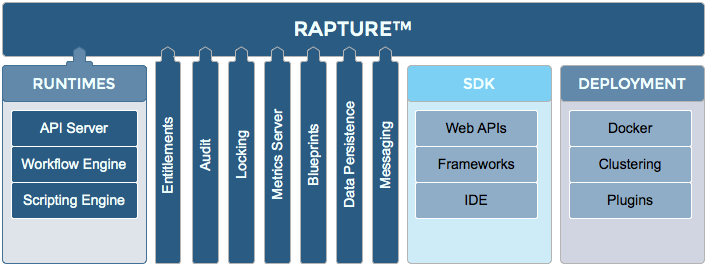
\includegraphics[width=15cm]{Graphics/rapturecore}
\caption{Rapture Component Parts}
\label{fig:RaptureDiagram}
\end{figure}

Applications that interact with \Rapture, or are \emph{hosted} on \Rapture will
use the \Rapture API to interact with this underlying framework. The goal of
the \Rapture API is that the interaction with \Rapture is invariant to the location
of the application -- the API looks \emph{the same} no matter where the application
resides.

\chapter{Application Locations}
Applications interacting with \Rapture will typicall fall within one of the
following categories.

\begin{itemize}
  \item{Client applications interacting with a remote \Rapture environment.}
  \item{Client \Reflex scripts using the ReflexRunner application.}
  \item{Server applications embedding the \Rapture kernel.}
  \item{Scripts running on a server that is itself running the \Rapture kernel.}
  \item{Extensions to \Reflex or repository or message drivers.}
  \item{Scripts run in the context of an ajax call from a web browser.}
\end{itemize}

\section{Context and Entitlements}
Every interaction with a \Rapture API call is made in the context of a logged in
user. That user, and its entitlement group membership and the parameters passed
to the call are used to determine whether the call can proceed or not. If an
API call is used to run a script on \Rapture or to start a workflow \emph{that} script
or workflow is run in the context of the calling user as well.

In some API use categories the interface used to interact with the \Rapture API
is already bound to a user - typically this is for processes that are running
server side. Client side use cases usually have to \emph{login} to \Rapture first,
providing credentials that get translated by the \Rapture API into a \verb+CallingContext+
value (a token) which can then be used in subsequent calls to identify the user
making the call. In some client side languages there are helper constructs that
can be used to automatically pass in the logged in context to the API calls,
leaving the programmer free to not worry about this aspect.

Wrapper applications such as ReflexRunner log in on the caller's behalf and then
pass that logged in API context to the underlying container that runs the script.

\section{Custom client applications}

Client applications that talk to \Rapture can be written in any of these supported languages as
long as the application can reach (using TCP/IP) a \Rapture API Server.

\begin{itemize}
  \item{Java (or anything that runs on the Java VM and can access Java classes.)}
  \item{.NET}
  \item{Python}
  \item{Javascript (typically node.js, see a later section on architectures for browser applications.)}
  \item{Ruby}
  \item{Go(lang)}
\end{itemize}

The transport between client and server uses a JSON-RPC style of communication which
means that other language support can easily be added. The build process for
\Rapture can autogenerate client side stubs once an initial template has been
created - the authors created the .NET implementation in a few hours.

Typically the use of \Rapture in these applications follows this pattern:

\begin{enumerate}
  \item{Obtain the ip address or name of the \Rapture environment API endpoint.}
  \item{Obtain the user name and password for the use of the API.}
  \item{Call a login function to obtain a calling context.}
  \item{Pass that login context into a wrapper (for future API use) or simply pass the context into future API calls.}
\end{enumerate}

For example in Java here is a simple code extract for the login and API use process:

\begin{lstlisting}[caption={Java simple example}, language=Java]
  String host = "test.incapture.net";
  String username = "test";
  String password = "secret";
  SimpleCredentialsProvider creds = new SimpleCredentialsProvider(username, password);
  HttpLoginApi loginApi = new HttpLoginApi(host, creds);
  loginApi.login();

  ScriptClient client = new ScriptClient(loginApi);
  String content = client.getDoc().getContent("//testRepo/doc/one");
  System.out.println(content);
\end{lstlisting}

This example logs into a \Rapture environment and passes that logged in context to a \verb+ScriptClient+
instance. It is this script client that can then be easily used to interact with \Rapture. The
\verb+getContent+ call in the document API will be described in detail later.

In Python, the equivalent interaction is reproduced below:

\begin{lstlisting}[caption={Python simple example}, language=Python]
  import raptureAPI
  url = 'test.incapture.net'
  username = 'test'
  password = 'secret'
  rapture = raptureAPI.raptureAPI(url, username, password)
  content = rapture.doDoc_GetContent('//testRepo/doc/one')
  print content
\end{lstlisting}

Here we see a similar login approach and then the invocation of the same \Rapture
API call. With the same target \Rapture environment these two code snippets will
produce exactly the same output.

\section{Client \Reflex scripts}

\Reflex scripts running on the client (or the server) are always running in a
container that has already been connected to an environment -- the wrapper is
the piece of code that has logged into \Rapture already.

In \Reflex then the code is even simpler. In fact \Reflex has some additional
syntax sugar for loading documents from \Rapture.

\begin{lstlisting}[caption={Reflex simple example}, language=reflex]
  contentAsMap <-- "//testRepo/doc/one";
  println(contentAsMap);

  // or

  content = #doc.getContent("//testRepo/doc/one");
  contentAsMap = fromjson(content);
  println(contentAsMap);
\end{lstlisting}

In the second access example we convert the raw JSON formatted document from
\Rapture into a \Reflex map structure so as to make the two approaches produce
the same output.

\section{Server side kernel applications}

If a Java (or Java VM) application embeds the \Rapture kernel code within it the
means for calling the \Rapture API can have a number of forms. Code running within
\Rapture has to be much more careful about calling contexts and who is actually
making the call, and there is no need to worry about host urls because the code
is running directly on \Rapture.

One approach to running the same example code is reproduced below:

\begin{lstlisting}[caption={Kernel simple example}, language=Java]
   CallingContext userContext = Kernel.getLogin().login(
          "test", "secret", null);
   String content = Kernel.getDoc().getContent(
          userContext, "//testRepo/doc/one");
   System.out.println(content);
\end{lstlisting}

Note that to run the above code your server application will have had to initialize
and configure itself first, something which is outside the scope of this document
but will trivially be a matter of defining configuration files for connection to
underlying data stores and then calling:

\begin{lstlisting}[caption={Kernel initialization}, language=Java]
   Kernel.initBootstrap();
\end{lstlisting}

\chapter{Application Location Summary}
Applications can sit in many places in the architecture of a solution that
includes a \Rapture system. The goal of the \Rapture API is to make the access
to \Rapture as simple and consistent as possible to all applications so it is
easy for a developer to move their applications within the system architecture or
to switch and change the programming languages used for an application.

\part{API}
\chapter{API Introduction}
The \Rapture API is divided into a number of sections. We've seen in an earlier
section how you may need to use the \emph{login} api to establish a connection
to \Rapture. The other sections of the API will form the rest of this document.
For each section the general positioning of the section with respect to \Rapture
will be described and then the detailed API calls will follow.

\section{Doc API}
Plugins in \Rapture are installable items that can be released to a \Rapture environment in
a consistent way. There are three parts to the Plugin API.

The first part relates to retrieving information about what is actually installed, and what items were installed with each
plugin. These are used by operator consoles and are informational.

The second part relates to installing an actual plugin. These calls are typically used by a specific
client side application "PluginInstaller" or a self installing library that uses the "SelfPluginInstallerLib". Plugins
defined in this way are jar archives that have a very specific structure. Typically a developer lays out this structure
in the file system and then uses a build process to package this information up into a jar file which can then be used with
the PluginInstaller application.

\section{File layout of a plugin}

A sample layout of a plugin "on disk" is reproduced below:

\begin{Verbatim}
  -- src/main/resources
     - PLUGIN
        - plugin.txt
        - content
          - testRepo
             - .rdoc
             someContent.rdoc
          - myscripts
             - test.script
\end{Verbatim}

The mandatory aspects of a plugin are the concept of a PLUGIN folder in the resources within
which is a plugin.txt file. This file has a specific format, an example is reproduced below:

\begin{Verbatim}
  {
     "depends":{},
     "description":"Curtis Web Core",
     "plugin":"CurtisWebCore",
     "version":{
     		"major":1,
     		"minor":1,
     		"release":32,
     		"timestamp":99999999999999
     }
  }
\end{Verbatim}

Most of these fields are self describing - the "plugin" field is the unique reference (uri) of this
plugin and the version section defines the version \emph{of this plugin}. The description is for operators
and the depends field can contain a map of other plugins and their version numbers required.

\section{Plugin file types}

The content folder contains information and definitions for content and configuration that this plugin defines. The
file name extension defines what the plugin installer will do for this item.

\begin{table}[H]
\begin{center}
\begin{tabular}{r p{10cm}}
  Extension & Purpose \\
  \hline
  script & Defines a \Reflex script. The full uri of the script is formed from this file's location in the content directory.\\
  series & Defines set of points in a series (if fully named) or the definition of a series repository. In the latter case the .series file
     must be at the 2nd top level folder in the content folder - the name of the folder is the name of the repository in \Rapture. \\
  blob & Defines a blob in a blob repository or the definition of a blob repository (if the file is .blob). Note that files that are not in
    the list of extensions in this table are treated as blobs, with the mime type inferred from the extension of the file. \\
  rdoc & Defines a document in a document repository \emph{or} the definition of a document repository (if no name specified). \\
  idgen & Defines an idgenerator. The name of the generator is defined by the top level folder, the contents is the configuration of an ID generator.\\
  revent & Defines a rapture event. The content of the file is a RaptureEvent structure (as json). \\
  table & Defines a rapture table. The name of the table is the enclosing folder. \\
  job & Defines a schedule job. \\
  workflow & Defines a workflow. \\
  lock & Defines a lock manager. \\
  structured & Defines a structure store reference. \\
\end{tabular}
\end{center}
\end{table}

In all cases for these files where the content drives the definition of something in \Rapture, the content is
a json formatted document that is the equivalent of serializing the result of the appropriate "get" call for that entity.

For example, the document "getDocRepoConfig" call returns a "DocumentRepoConfig" which has a complex structure of
information about the description, document repo configuration and so on. In a file format this will look as follows:

\begin{Verbatim}
  {
    "authority":"curtis.menu",
    "strictCheck":true,
    "indexes":[],
    "fullTextIndexes":[],
    "documentRepo":
       {
          "authority":"curtis.menu",
          "config":"NREP {} USING MONGODB { prefix=\"curtis.menu\" }"
       }
  }
\end{Verbatim}

To obtain the format for this you could also use the following \Reflex code:

\begin{Verbatim}
   config = #document.getDocRepoConfig('//curtis.menu');
   println(json(config));
\end{Verbatim}

The same technique can be used with other entity types.

\section{Plugin Build Process}
To build a plugin that has the resource configuration reproduced above the following
\emph{gradle} build process is recommended:

\begin{Verbatim}[fontsize=\footnotesize]
  raptureVersion = "3.0.0"

  apply plugin: 'application'

  dependencies {
          compile "net.rapture:SelfPluginInstallerLib:$raptureVersion"
  }

  mainClassName = "rapture.plugin.app.SelfInstaller"

  task fatJar(type: Jar) {
       manifest {
          attributes 'Implementation-Title' : 'Plugin self installer',
                     'Implementation-Version' : '1.0.0',
                     'Main-Class' : mainClassName
      }
      baseName = project.name
      from {
          configurations.compile.collect {
               it.isDirectory() ? it : zipTree(it) }
      } with jar
  }

  fatJar.dependsOn(compileJava)

\end{Verbatim}

This (simplified) build script uses the \Rapture open source SelfInstaller library which contains
a main entry point that can be used to install the plugin into a \Rapture environment.

Running \verb+gradle fatJar+ will create a single jar that can be invoked with 'java -jar' along with
the following command line options to connect it to a \Rapture environment. The self installer will use
the Plugin API described here to install the components registered in this Plugin.

\begin{table}[H]
\begin{center}
\begin{tabular}{r l p{10cm}}
  Extension & Purpose \\
  \hline
  \verb+--host+ & The \Rapture host to connect to. \\
  \verb+--user+ & The \Rapture user to connect as. \\
  \verb+--password+ & The \Rapture password to use for that user. \\
  \verb+--overlay+ & What overlay to use (optional) (see below). \\
\end{tabular}
\end{center}
\end{table}

\section{Plugin overlays}
A plugin file can contain other sections in addition to the "content" folder described above. These are known
as overlays and this can be used to combine the "default" content folder with a given overlay. Overlays are used
to perhaps define slightly different configuration documents for a development environment to a production environment -- in this case
the documents describing production changes would be specified in a "prod" folder - the sub contents following the same format
in style as the content folder. If this folder exists then passing \verb+--overlay prod+ to an installer would instruct the installer
to apply the content folder first, and then overlay the prod folder onto that, creating a merged view of what should be
installed for this plugin on this environment.

\section{Creating plugins from existing content}
The Plugin API contains calls that can be used when a \Rapture environment has existing content and configuration that needs to be captured in plugin format.

The basic approach is to first create a manifest (\Verb+createManifest+) and then add items to that manifest using the \Verb+add+ calls.
The version of the plugin needs to be set using \Verb+setManifestVersion+ and then the complete plugin is exported using \Verb+exportPlugin+. The content generated
is then of a form that can be installed using the PluginInstaller tool on a different environment, or extracted to be copied into a more
traditional Plugin project described above.

\subsubsection{ValidateDocRepo}
\label{Api:ValidateDocRepo}
\begin{verbatim}
   boolean validateDocRepo (
           String    docRepoUri
   )
\end{verbatim}
\begin{lstlisting}[language=reflex]
// Reflex use
ret = #doc.validateDocRepo(docRepoUri);
\end{lstlisting}
Validate Doc Repo information




\rule{15cm}{2pt}
\subsubsection{CreateDocRepo}
\label{Api:CreateDocRepo}
\begin{verbatim}
   void createDocRepo (
           String    docRepoUri
           String    config
   )
\end{verbatim}
\begin{lstlisting}[language=reflex]
// Reflex use
ret = #doc.createDocRepo(docRepoUri,config);
\end{lstlisting}
The \verb+createDocRepo+ is used to create a new document repository in \Rapture. The parameters to the call
look straightforward -- simply the name of the new repository and a configuration string. The configuration string is
in fact a complex instruction written in a repository domain specific language (DSL) that is used to define the
capabilities and underlying implementation of the repository.

The typical configuration string for a versioned repository backed by MongoDB is reproduced below:

\begin{Verbatim}
NREP {} USING MONGODB { prefix = 'test' }
\end{Verbatim}

The general form of the configuration is:

\begin{Verbatim}
[type of document repo] { [ document repo config] }
     USING [underlying implementation] { [ config ]}
     [ ON [ instance] ]
\end{Verbatim}

The first part, the type of the document repo, can be either \verb+NREP+ or \verb+REP+. The former
indicates that a versioned repository should be created, the latter that an unversioned repository
should be created.

The document repo config part of the configuration string is currently blank for all document repo types.

The second part of the configuration string defines the underlying implementation and its configuration. In
most cases the configuration associated with the implementation has a \verb+prefix+ parameter that is used to
define a table or a collection or a prefix for such entities in the underlying storage. The underlying implementation
defines what lower level software is used to host the data managed by \Rapture. The following table shows the current
implementations:

\begin{table}[h]
\begin{center}
\begin{tabular}{r l p{8cm}}
  Keyword & Underlying & Configuration \\
  \hline
  MONGODB & MongoDb & The prefix parameter defines the name of the collections used by this repository. To avoid
  conflict this is usually a function of the name of the \Rapture repository. \\
  CASSANDRA & Cassandra & The prefix parameter defines the name of the collections used by this repository. To avoid
  conflict this is usually a function of the name of the \Rapture repository. \\
  POSTGRES & PostgresSql &  The prefix parameter defines the name of the tables used by this repository. To avoid
  conflict this is usually a function of the name of the \Rapture repository. \\
\end{tabular}
\end{center}
\end{table}

Incapture has additional implementations of document repositories for Oracle, JDBC, Redis, ehCache and memcached.

There are some additional directives that can be used in a repository configuration definition.

If the keyword \verb+READONLY+ is used at the start of the configuration (e.g. \verb+READONLY NREP ...+) the repository will
be readonly -- it is assumed that either a different repository configuration is used to write data (and they
share the same \verb+preifx+ but different entitlements) or the underlying data in a repository is a backup of
a repository created with a different system. In any case the \verb+READONLY+ keyword makes all writing API calls to
this repository fail with an exception being thrown.

The \verb+ON+ directive defines which configuration will be used to connect to the underlying store. If
not present the \verb+DEFAULT+ configuration will be used. These keywords are used by the underlying
implementation to load a system specific configuration file, environment variables or property set.

For example the default configuration for MongoDb (\verb+ON DEFAULT+) instructs the MongoDB implementation
to look in three places for a connection string to a MongoDB server -

\begin{itemize}
\item{The environment variable RAPTUREMONGODB-DEFAULT.}
\item{The java property RAPTUREMONGODB-DEFAULT.}
\item{The line beginning default= in the file RaptureMONGODB.cfg on the classpath of the application.}
\end{itemize}

In most cases the implementation will read the value from the file associated with the application server.

Using this technique multiple underlying servers can be used and repositories attached to them using the
\verb+ON+ keyword.



\rule{15cm}{2pt}
\subsubsection{DocRepoExists}
\label{Api:DocRepoExists}
\begin{verbatim}
   boolean docRepoExists (
           String    docRepoUri
   )
\end{verbatim}
\begin{lstlisting}[language=reflex]
// Reflex use
ret = #doc.docRepoExists(docRepoUri);
\end{lstlisting}
The \verb+docRepoExists+ call is used to test whether a given named repository is known
to the \Rapture environment. The method takes a single repo name as a parameter and returns
true or false according to an existence check. This call is typically used in an installation
script to determine whether a repository should be created using the \verb+createDocRepo+ call.



\rule{15cm}{2pt}
\subsubsection{DocExists}
\label{Api:DocExists}
\begin{verbatim}
   boolean docExists (
           String    docUri
   )
\end{verbatim}
\begin{lstlisting}[language=reflex]
// Reflex use
ret = #doc.docExists(docUri);
\end{lstlisting}
The \verb+docExists+ API call is used to determine whether there is a document
in a \Rapture system at a given uri. The call is usually more efficient than
attempting to retrieve a document depending on the underlying implementation
of the driver for the repository storage.



\rule{15cm}{2pt}
\subsubsection{GetDocRepoConfig}
\label{Api:GetDocRepoConfig}
\begin{verbatim}
   DocumentRepoConfig getDocRepoConfig (
           String    docRepoUri
   )
\end{verbatim}
\begin{lstlisting}[language=reflex]
// Reflex use
ret = #doc.getDocRepoConfig(docRepoUri);
\end{lstlisting}
Get Doc Repo Config




\rule{15cm}{2pt}
\subsubsection{GetDocRepoStatus}
\label{Api:GetDocRepoStatus}
\begin{verbatim}
   Map<String,String> getDocRepoStatus (
           String    docRepoUri
   )
\end{verbatim}
\begin{lstlisting}[language=reflex]
// Reflex use
ret = #doc.getDocRepoStatus(docRepoUri);
\end{lstlisting}
Get Doc Repo Status




\rule{15cm}{2pt}
\subsubsection{GetDocRepoConfigs}
\label{Api:GetDocRepoConfigs}
\begin{verbatim}
   List<DocumentRepoConfig> getDocRepoConfigs (
   )
\end{verbatim}
\begin{lstlisting}[language=reflex]
// Reflex use
ret = #doc.getDocRepoConfigs();
\end{lstlisting}
The \verb+getDocRepoConfigs+ call returns all of the document repository configurations in use
on a \Rapture server. This call is often used in management user interfaces to provide a high level
starting point for navigating a \Rapture environment.

The object returned in a list from this function is described as part of the \verb+getDocRepoConfig+ call.



\rule{15cm}{2pt}
\subsubsection{DeleteDocRepo}
\label{Api:DeleteDocRepo}
\begin{verbatim}
   void deleteDocRepo (
           String    docRepoUri
   )
\end{verbatim}
\begin{lstlisting}[language=reflex]
// Reflex use
ret = #doc.deleteDocRepo(docRepoUri);
\end{lstlisting}
The \verb+deleteDocRepo+ call removes a document repository from a \Rapture system. The underlying
implementation of a repository driver determines whether the data associated with this repository
is also removed from the system.



\rule{15cm}{2pt}
\subsubsection{ArchiveRepoDocs}
\label{Api:ArchiveRepoDocs}
\begin{verbatim}
   void archiveRepoDocs (
           String    docRepoUri
           int    versionLimit
           long    timeLimit
           boolean    ensureVersionLimit
   )
\end{verbatim}
\begin{lstlisting}[language=reflex]
// Reflex use
ret = #doc.archiveRepoDocs(docRepoUri,versionLimit,timeLimit,ensureVersionLimit);
\end{lstlisting}
The \verb+archiveRepoDocs+ call removes older versions of documents from a
repository that match certain criteria.

\begin{table}[H]
  \small
\begin{center}
\begin{tabular}{r p{8cm}}
  Parameter & Purpose \\
  \hline
  docRepoUri & If this document uri contains just the name of a repository then all
  documents in the repository will be checked. Otherwise just those matching this prefix will be
  scanned. \\
  versionLimit & If the ensureVersionLimit parameter is true this parameter will determine
  the minimum number of versions to keep fora document. \\
  timeLimit & This parameter determines the modification time of the oldest version to keep during this
  archive process. \\
  ensureVersionLimit & If this parameter is true the versionLimit parameter is used \\
\end{tabular}
\end{center}
\end{table}



\rule{15cm}{2pt}
\subsubsection{GetDocAndMeta}
\label{Api:GetDocAndMeta}
\begin{verbatim}
   DocumentWithMeta getDocAndMeta (
           String    docUri
   )
\end{verbatim}
\begin{lstlisting}[language=reflex]
// Reflex use
ret = #doc.getDocAndMeta(docUri);
\end{lstlisting}
The \verb+getDocAndMeta+ API call is used to retrieve both the content of
a document and the meta data associated with that document. If the uri does
not have a version qualifier the information returned will refer to the latest
version of the document. The return value is complex is structure -- please
refer to the table at the end of this section to understand the fields within that
structure.

The \verb+DocumentWithMeta+ return value is a complex structure that contains
the following fields:

\begin{table}[h]
\begin{center}
\begin{tabular}{rl p{8cm}}
  Field & Type & Description \\
  \hline
  displayName & String & the url of this document \\
  metaData & DocumentMetaData & the metadata associated with this document \\
  content & String & the content of this document \\
\end{tabular}
\end{center}
\end{table}



\rule{15cm}{2pt}
\subsubsection{GetDocMeta}
\label{Api:GetDocMeta}
\begin{verbatim}
   DocumentMetadata getDocMeta (
           String    docUri
   )
\end{verbatim}
\begin{lstlisting}[language=reflex]
// Reflex use
ret = #doc.getDocMeta(docUri);
\end{lstlisting}
The \verb+getDocMeta+ API call is used to retrieve the meta data associated
with a given document in a repository. If the uri does not have a version
qualifier the information returned will refer to the latest version of the
document. The return value is complex is structure -- please refer to the
table at the end of this section to understand the fields within that
structure.

The \verb+DocumentMetaData+ return value is a complex structure that contains
the following fields:

\begin{table}[h]
\begin{center}
\begin{tabular}{rl p{8cm}}
  Field & Type & Description \\
  \hline
  version & integer & the version number of this document \\
  createdTimestamp & long & when this document was first created \\
  modifiedTimestamp & long & when this document was last modified \\
  user & string & the user that made this modification \\
  comment & string & any comment that was provided when the document was written \\
  deleted & boolean & whether this document is deleted \\
\end{tabular}
\end{center}
\end{table}



\rule{15cm}{2pt}
\subsubsection{RevertDoc}
\label{Api:RevertDoc}
\begin{verbatim}
   DocumentWithMeta revertDoc (
           String    docUri
   )
\end{verbatim}
\begin{lstlisting}[language=reflex]
// Reflex use
ret = #doc.revertDoc(docUri);
\end{lstlisting}
The \verb+revertDoc+ call loads the previous version of a document and saves
that as the latest version. It will create a new version so that audit
history is preserved.



\rule{15cm}{2pt}
\subsubsection{GetDoc}
\label{Api:GetDoc}
\begin{verbatim}
   String getDoc (
           String    docUri
   )
\end{verbatim}
\begin{lstlisting}[language=reflex]
// Reflex use
ret = #doc.getDoc(docUri);
\end{lstlisting}
The \verb+getDoc+ API call is used to retrieve content from a document repository
in \Rapture. The single parameter \verb+docUri+ is a string that defines the
location of the document within the \Rapture system. It can optionally be
prefixed with the \verb+document:+ scheme qualifier. Depending on the client
side implementation the call can throw an exception if the repository is not
existent or the entitlements of the server prohibit such access. Some implementations
wrap the document does not exist failure into returning a null value from this
API call.

In the \Reflex scripting language a caller can use the \emph{pull} operator (\verb+<--+)
to retrieve a document from \Rapture and convert its contents from JSON to a \Reflex map
of maps. This call will fail if the document is not in JSON format.



\rule{15cm}{2pt}
\subsubsection{PutDoc}
\label{Api:PutDoc}
\begin{verbatim}
   String putDoc (
           String    docUri
           String    content
   )
\end{verbatim}
\begin{lstlisting}[language=reflex]
// Reflex use
ret = #doc.putDoc(docUri,content);
\end{lstlisting}
The \verb+putDoc+ call writes data into a \Rapture document repository. The
data in a document repository is a simple string but this is usually formatted
as a JSON document. If the repository is versioned this call will write a new
version to the repository and set the latest version to be this version. If it
is not versioned this call will simply overwrite the current version.

If there is no document at this location the call will create a new document.

If the repository has an id generator attached to it (see the id API) the uri
can end in the special keyword \verb+#id+ a new unique id will be generated when
this document is written. The return value of this API call will then reflect
the actual location that was used to store this content.



\rule{15cm}{2pt}
\subsubsection{PutDocWithVersion}
\label{Api:PutDocWithVersion}
\begin{verbatim}
   boolean putDocWithVersion (
           String    docUri
           String    content
           int    currentVersion
   )
\end{verbatim}
\begin{lstlisting}[language=reflex]
// Reflex use
ret = #doc.putDocWithVersion(docUri,content,currentVersion);
\end{lstlisting}
The \verb+putDocWithVersion+ can be used to implement an optimistic locking
strategy for updating data into a repository. The approach is for an application
to load a document with its version using the \verb+getDocAndMeta+ call. The
application can then modify that document and use this call to store the
update, passing in the last known version. The call will succeed if and only if
no other program has modified the document -- in which case the version number
of the document will be incremented and not match.

If the version check fails the call will fail with an exception that will be
returned to the caller in a manner appropriate to the calling language implementation.



\rule{15cm}{2pt}
\subsubsection{PutDocWithEventContext}
\label{Api:PutDocWithEventContext}
\begin{verbatim}
   DocWriteHandle putDocWithEventContext (
           String    docUri
           String    content
           Map<String,String>    eventContext
   )
\end{verbatim}
\begin{lstlisting}[language=reflex]
// Reflex use
ret = #doc.putDocWithEventContext(docUri,content,eventContext);
\end{lstlisting}
The \verb+putDocWithEventContext+ call is identical to \verb+putDoc+ except that
any events created by the act of storing this data will contain additional information
that is passed as the \verb+eventContext+ parameter. See \emph{Events} for more details
on how events are fired and attached to.



\rule{15cm}{2pt}
\subsubsection{DeleteDoc}
\label{Api:DeleteDoc}
\begin{verbatim}
   boolean deleteDoc (
           String    docUri
   )
\end{verbatim}
\begin{lstlisting}[language=reflex]
// Reflex use
ret = #doc.deleteDoc(docUri);
\end{lstlisting}
The \verb+deleteDoc+ call is used to remove a document from a document repository.

In a versioned repository the history of the document is preserved -- the effect of
this call is to set the \emph{current} version of the document to a null version, so
that \verb+getDoc+ and \verb+existsDoc+ calls work as expected, but you can retrieve
old versions of the document.



\rule{15cm}{2pt}
\subsubsection{RenameDoc}
\label{Api:RenameDoc}
\begin{verbatim}
   String renameDoc (
           String    fromDocUri
           String    toDocUri
   )
\end{verbatim}
\begin{lstlisting}[language=reflex]
// Reflex use
ret = #doc.renameDoc(fromDocUri,toDocUri);
\end{lstlisting}
The \verb+renameDoc+ call is an atomic wrapper around the \verb+deleteDoc+ and \verb+putDoc+.

The implementation simply retrieves the original document contents using
\verb+getDoc+ and then stores the document using \verb+putDoc+. Finally
the original document is deleted using \verb+deleteDoc+.

The entitlements check for this call also checks the entitlements for the
three calls it makes.



\rule{15cm}{2pt}
\subsubsection{GetDocs}
\label{Api:GetDocs}
\begin{verbatim}
   Map<String,String> getDocs (
           List<String>    docUris
   )
\end{verbatim}
\begin{lstlisting}[language=reflex]
// Reflex use
ret = #doc.getDocs(docUris);
\end{lstlisting}
The \verb+getDocs+ call takes a list of document uris and performs a \verb+getDoc+ call
on each uri. If the call passes the entitlement check for \verb+getDoc+ with that
uri the content is loaded and the added to the return map, keyed by the uri.



\rule{15cm}{2pt}
\subsubsection{GetDocAndMetas}
\label{Api:GetDocAndMetas}
\begin{verbatim}
   List<DocumentWithMeta> getDocAndMetas (
           List<String>    docUris
   )
\end{verbatim}
\begin{lstlisting}[language=reflex]
// Reflex use
ret = #doc.getDocAndMetas(docUris);
\end{lstlisting}
The \verb+getDocAndMetas+ call is a batch form of \verb+getDocAndMeta+. The return
value is the result of calling that function for each uri in the list passed to
the batch call and adding it to the return list. If the entitlement check fails
for the individual call a null is placed in the list at that point.



\rule{15cm}{2pt}
\subsubsection{DocsExist}
\label{Api:DocsExist}
\begin{verbatim}
   List<boolean> docsExist (
           List<String>    docUris
   )
\end{verbatim}
\begin{lstlisting}[language=reflex]
// Reflex use
ret = #doc.docsExist(docUris);
\end{lstlisting}
The \verb+docExists+ call is a batch form of the \verb+docExists+ call.

For each uri in the parameter to the call the \verb+docExists+ call is made
after an entitlement check. The return value of the call is added to the list
returned by this function. If the entitlement check fails a false is placed
in its position in the return list.



\rule{15cm}{2pt}
\subsubsection{PutDocs}
\label{Api:PutDocs}
\begin{verbatim}
   List<Object> putDocs (
           List<String>    docUris
           List<String>    contents
   )
\end{verbatim}
\begin{lstlisting}[language=reflex]
// Reflex use
ret = #doc.putDocs(docUris,contents);
\end{lstlisting}
The \verb+putDocs+ call is a wrapper around a loop to the \verb+putDoc+ call. For each
uri/content pair the entitlements for a given store are checked. The return value
is a list of the resultant uris created by the store call -- which can contain autogenerated
ids as per the \verb+putDoc+ implementation.



\rule{15cm}{2pt}
\subsubsection{RenameDocs}
\label{Api:RenameDocs}
\begin{verbatim}
   List<String> renameDocs (
           String    authority
           String    comment
           List<String>    fromDocUris
           List<String>    toDocUris
   )
\end{verbatim}
\begin{lstlisting}[language=reflex]
// Reflex use
ret = #doc.renameDocs(authority,comment,fromDocUris,toDocUris);
\end{lstlisting}
The \verb+renameDocs+ call is a batch version of the \verb+renameDoc+ call.

The entitlement check for \verb+renameDoc+ is made for each uri in the batch. The
return value for \verb+renameDoc+ is added to the return list of this call. If
the entitlement check fails for a uri a null will occupy its place in the list.



\rule{15cm}{2pt}
\subsubsection{DeleteDocsByUriPrefix}
\label{Api:DeleteDocsByUriPrefix}
\begin{verbatim}
   List<String> deleteDocsByUriPrefix (
           String    docUri
   )
\end{verbatim}
\begin{lstlisting}[language=reflex]
// Reflex use
ret = #doc.deleteDocsByUriPrefix(docUri);
\end{lstlisting}
The \verb+deleteDocsByUriPrefix+ call is used to remove all documents below a certain
point in the hierarchy implied by the uri naming scheme. In conceptual terms it is
the equivalent of "removing the folder" from a repository.



\rule{15cm}{2pt}
\subsubsection{ListDocsByUriPrefix}
\label{Api:ListDocsByUriPrefix}
\begin{verbatim}
   Map<String,RaptureFolderInfo> listDocsByUriPrefix (
           String    docUri
           int    depth
   )
\end{verbatim}
\begin{lstlisting}[language=reflex]
// Reflex use
ret = #doc.listDocsByUriPrefix(docUri,depth);
\end{lstlisting}
The \verb+listDocsByUriPrefix+ call is normally used by user interfaces that wish
to present a browser type interface on a document repository. The call returns all documents
and "sub folders" (to a given depth) below a given point in the hierarchy implied
by the naming conventions used in uris. Typically an interface will use \verb+/+ as
the initial prefix and then append onto that prefix the names of either documents
or folders for further \verb+listDocs+ type calls or \verb+getDoc+ if the location
maps to a real document.

The \verb+RaptureFolderInfo+ structure returned by this call is described below:

\begin{table}[H]
  \small
\begin{center}
\begin{tabular}{r l p{8cm}}
  Field & Type & Description \\
  \hline
  name & String & The name of this element. \\
  folder & Boolean & Whether the name refers to a document or a sub-folder \\
\end{tabular}
\end{center}
\end{table}



\rule{15cm}{2pt}
\subsubsection{SetDocAttribute}
\label{Api:SetDocAttribute}
\begin{verbatim}
   boolean setDocAttribute (
           String    attributeUri
           String    value
   )
\end{verbatim}
\begin{lstlisting}[language=reflex]
// Reflex use
ret = #doc.setDocAttribute(attributeUri,value);
\end{lstlisting}
The \verb+setDocAttribute+ call is used to add an attribute to a document in a repository.

Attributes are metadata that can be used to place any arbitrary value on a document independent of its
content.

In the call an attribute uri is the combination of a document path (as seen in many other calls) with a
bookmark symbol (\verb+#+) followed by the name of an attribute. The value is a string value that has
meaning to the calling application.

The return value is true if the attribute was set by the repository.



\rule{15cm}{2pt}
\subsubsection{SetDocAttributes}
\label{Api:SetDocAttributes}
\begin{verbatim}
   Map<String,boolean> setDocAttributes (
           String    attributeUri
           List<String>    keys
           List<String>    values
   )
\end{verbatim}
\begin{lstlisting}[language=reflex]
// Reflex use
ret = #doc.setDocAttributes(attributeUri,keys,values);
\end{lstlisting}
Set Dc Attributes




\rule{15cm}{2pt}
\subsubsection{GetDocAttribute}
\label{Api:GetDocAttribute}
\begin{verbatim}
   XferDocumentAttribute getDocAttribute (
           String    attributeUri
   )
\end{verbatim}
\begin{lstlisting}[language=reflex]
// Reflex use
ret = #doc.getDocAttribute(attributeUri);
\end{lstlisting}
The \verb+getDocAttribute+ call mirrors the \verb+setDocAttribute+ call. A full attributeUri is passed
and the return value contains both the key and the value associated with the uri.



\rule{15cm}{2pt}
\subsubsection{GetDocAttributes}
\label{Api:GetDocAttributes}
\begin{verbatim}
   List<XferDocumentAttribute> getDocAttributes (
           String    attributeUri
   )
\end{verbatim}
\begin{lstlisting}[language=reflex]
// Reflex use
ret = #doc.getDocAttributes(attributeUri);
\end{lstlisting}
Get Doc Attributes




\rule{15cm}{2pt}
\subsubsection{DeleteDocAttribute}
\label{Api:DeleteDocAttribute}
\begin{verbatim}
   boolean deleteDocAttribute (
           String    attributeUri
   )
\end{verbatim}
\begin{lstlisting}[language=reflex]
// Reflex use
ret = #doc.deleteDocAttribute(attributeUri);
\end{lstlisting}
The \verb+deleteDocAttribute+ call is used to remove an attribute previously added using
\verb+setDocAttribute+. It returns true if the attribute was deleted (usually always the case unless
the attribute did not exist).



\rule{15cm}{2pt}
\subsubsection{GetDocRepoIdGenUri}
\label{Api:GetDocRepoIdGenUri}
\begin{verbatim}
   String getDocRepoIdGenUri (
           String    docRepoUri
   )
\end{verbatim}
\begin{lstlisting}[language=reflex]
// Reflex use
ret = #doc.getDocRepoIdGenUri(docRepoUri);
\end{lstlisting}
Get Doc Repo




\rule{15cm}{2pt}
\subsubsection{SetDocRepoIdGenConfig}
\label{Api:SetDocRepoIdGenConfig}
\begin{verbatim}
   DocumentRepoConfig setDocRepoIdGenConfig (
           String    docRepoUri
           String    idGenConfig
   )
\end{verbatim}
\begin{lstlisting}[language=reflex]
// Reflex use
ret = #doc.setDocRepoIdGenConfig(docRepoUri,idGenConfig);
\end{lstlisting}
Document repositories can have an id generator attached to them. If a document is added to
a repository and it contains a "\verb+#id+" suffix the id generator will replace that keyword with
a newly generated unique id.

The \verb+setDocRepoIdGenConfig+ is used to define the configuration for such a generator.

In a manner similar to the general repository configuration an id generator is defined using
a configuration string that conforms to a domain specific language (DSL). A typical example is
reproduced below:

\begin{verbatim}
IDGEN {} USING MONGODB { prefix = 'testid' }
\end{verbatim}

In this example MongoDB is used as the id generator and this is the only option in the open
source version of \Rapture.



\rule{15cm}{2pt}
\subsubsection{GetDocRepoIdGenConfig}
\label{Api:GetDocRepoIdGenConfig}
\begin{verbatim}
   RaptureIdGenConfig getDocRepoIdGenConfig (
           String    docRepoUri
   )
\end{verbatim}
\begin{lstlisting}[language=reflex]
// Reflex use
ret = #doc.getDocRepoIdGenConfig(docRepoUri);
\end{lstlisting}
Get Doc Id 




\rule{15cm}{2pt}

\chapter{Blob API}
\index{Blob API}
Plugins in \Rapture are installable items that can be released to a \Rapture environment in
a consistent way. There are three parts to the Plugin API.

The first part relates to retrieving information about what is actually installed, and what items were installed with each
plugin. These are used by operator consoles and are informational.

The second part relates to installing an actual plugin. These calls are typically used by a specific
client side application "PluginInstaller" or a self installing library that uses the "SelfPluginInstallerLib". Plugins
defined in this way are jar archives that have a very specific structure. Typically a developer lays out this structure
in the file system and then uses a build process to package this information up into a jar file which can then be used with
the PluginInstaller application.

\section{File layout of a plugin}

A sample layout of a plugin "on disk" is reproduced below:

\begin{Verbatim}
  -- src/main/resources
     - PLUGIN
        - plugin.txt
        - content
          - testRepo
             - .rdoc
             someContent.rdoc
          - myscripts
             - test.script
\end{Verbatim}

The mandatory aspects of a plugin are the concept of a PLUGIN folder in the resources within
which is a plugin.txt file. This file has a specific format, an example is reproduced below:

\begin{Verbatim}
  {
     "depends":{},
     "description":"Curtis Web Core",
     "plugin":"CurtisWebCore",
     "version":{
     		"major":1,
     		"minor":1,
     		"release":32,
     		"timestamp":99999999999999
     }
  }
\end{Verbatim}

Most of these fields are self describing - the "plugin" field is the unique reference (uri) of this
plugin and the version section defines the version \emph{of this plugin}. The description is for operators
and the depends field can contain a map of other plugins and their version numbers required.

\section{Plugin file types}

The content folder contains information and definitions for content and configuration that this plugin defines. The
file name extension defines what the plugin installer will do for this item.

\begin{table}[H]
\begin{center}
\begin{tabular}{r p{10cm}}
  Extension & Purpose \\
  \hline
  script & Defines a \Reflex script. The full uri of the script is formed from this file's location in the content directory.\\
  series & Defines set of points in a series (if fully named) or the definition of a series repository. In the latter case the .series file
     must be at the 2nd top level folder in the content folder - the name of the folder is the name of the repository in \Rapture. \\
  blob & Defines a blob in a blob repository or the definition of a blob repository (if the file is .blob). Note that files that are not in
    the list of extensions in this table are treated as blobs, with the mime type inferred from the extension of the file. \\
  rdoc & Defines a document in a document repository \emph{or} the definition of a document repository (if no name specified). \\
  idgen & Defines an idgenerator. The name of the generator is defined by the top level folder, the contents is the configuration of an ID generator.\\
  revent & Defines a rapture event. The content of the file is a RaptureEvent structure (as json). \\
  table & Defines a rapture table. The name of the table is the enclosing folder. \\
  job & Defines a schedule job. \\
  workflow & Defines a workflow. \\
  lock & Defines a lock manager. \\
  structured & Defines a structure store reference. \\
\end{tabular}
\end{center}
\end{table}

In all cases for these files where the content drives the definition of something in \Rapture, the content is
a json formatted document that is the equivalent of serializing the result of the appropriate "get" call for that entity.

For example, the document "getDocRepoConfig" call returns a "DocumentRepoConfig" which has a complex structure of
information about the description, document repo configuration and so on. In a file format this will look as follows:

\begin{Verbatim}
  {
    "authority":"curtis.menu",
    "strictCheck":true,
    "indexes":[],
    "fullTextIndexes":[],
    "documentRepo":
       {
          "authority":"curtis.menu",
          "config":"NREP {} USING MONGODB { prefix=\"curtis.menu\" }"
       }
  }
\end{Verbatim}

To obtain the format for this you could also use the following \Reflex code:

\begin{Verbatim}
   config = #document.getDocRepoConfig('//curtis.menu');
   println(json(config));
\end{Verbatim}

The same technique can be used with other entity types.

\section{Plugin Build Process}
To build a plugin that has the resource configuration reproduced above the following
\emph{gradle} build process is recommended:

\begin{Verbatim}[fontsize=\footnotesize]
  raptureVersion = "3.0.0"

  apply plugin: 'application'

  dependencies {
          compile "net.rapture:SelfPluginInstallerLib:$raptureVersion"
  }

  mainClassName = "rapture.plugin.app.SelfInstaller"

  task fatJar(type: Jar) {
       manifest {
          attributes 'Implementation-Title' : 'Plugin self installer',
                     'Implementation-Version' : '1.0.0',
                     'Main-Class' : mainClassName
      }
      baseName = project.name
      from {
          configurations.compile.collect {
               it.isDirectory() ? it : zipTree(it) }
      } with jar
  }

  fatJar.dependsOn(compileJava)

\end{Verbatim}

This (simplified) build script uses the \Rapture open source SelfInstaller library which contains
a main entry point that can be used to install the plugin into a \Rapture environment.

Running \verb+gradle fatJar+ will create a single jar that can be invoked with 'java -jar' along with
the following command line options to connect it to a \Rapture environment. The self installer will use
the Plugin API described here to install the components registered in this Plugin.

\begin{table}[H]
\begin{center}
\begin{tabular}{r l p{10cm}}
  Extension & Purpose \\
  \hline
  \verb+--host+ & The \Rapture host to connect to. \\
  \verb+--user+ & The \Rapture user to connect as. \\
  \verb+--password+ & The \Rapture password to use for that user. \\
  \verb+--overlay+ & What overlay to use (optional) (see below). \\
\end{tabular}
\end{center}
\end{table}

\section{Plugin overlays}
A plugin file can contain other sections in addition to the "content" folder described above. These are known
as overlays and this can be used to combine the "default" content folder with a given overlay. Overlays are used
to perhaps define slightly different configuration documents for a development environment to a production environment -- in this case
the documents describing production changes would be specified in a "prod" folder - the sub contents following the same format
in style as the content folder. If this folder exists then passing \verb+--overlay prod+ to an installer would instruct the installer
to apply the content folder first, and then overlay the prod folder onto that, creating a merged view of what should be
installed for this plugin on this environment.

\section{Creating plugins from existing content}
The Plugin API contains calls that can be used when a \Rapture environment has existing content and configuration that needs to be captured in plugin format.

The basic approach is to first create a manifest (\Verb+createManifest+) and then add items to that manifest using the \Verb+add+ calls.
The version of the plugin needs to be set using \Verb+setManifestVersion+ and then the complete plugin is exported using \Verb+exportPlugin+. The content generated
is then of a form that can be installed using the PluginInstaller tool on a different environment, or extracted to be copied into a more
traditional Plugin project described above.

\subsection{CreateBlobRepo}
\index{CreateBlobRepo}
\label{Api:CreateBlobRepo}
\begin{Verbatim}
   void createBlobRepo (
           String    blobRepoUri
           String    config
           String    metaConfig
   )
\end{Verbatim}
\begin{Verbatim}[formatcom=\color{Maroon}]
  Entitlement: /repo/write
\end{Verbatim}
%\begin{lstlisting}[language=reflex]
%ret = #blob.createBlobRepo(blobRepoUri,config,metaConfig);
%\end{lstlisting}
The \verb+createBlobRepo+ is used to create a new blob repository in \Rapture. The two configuration strings
act in a similar way to the Document API's \verb+createDocRepo+ call, in fact the \verb+metaConfig+ parameter
is used to define an internal document repository that will be used to store and manage the meta data for the
repository. The documentation for \verb+createDocRepo+ shows the possible options for that configuration.

The main configuration string is a similar domain specific language that is used to pass configuration
options to an underlying implementation. The current options are simply described with an example.

The typical configuration string for a blob repository backed by MongoDB is reproduced below:

\begin{verbatim}
BLOB {} USING MONGODB { prefix = 'testBlob' }
\end{verbatim}

The general form of the configuration is:

\begin{verbatim}
BLOB { [ blob repo config] }
     USING [underlying implementation] { [ config ]}
     [ ON [ instance] ]
\end{verbatim}

The blob repo config part of the configuration string is currently blank for all blob repo types.

The second part of the configuration string defines the underlying implementation and its configuration. In
most cases the configuration associated with the implementation has a \verb+prefix+ parameter that is used to
define a table or a collection or a prefix for such entities in the underlying storage. The underlying implementation
defines what lower level software is used to host the data managed by \Rapture. The following table shows the current
implementations:

\begin{table}[h]
  \small
\begin{center}
\begin{tabular}{r l p{7cm}}
  Keyword & Underlying & Configuration \\
  \hline
  MONGODB & MongoDb & The prefix parameter defines the name of the collections used by this repository. To avoid
  conflict this is usually a function of the name of the \Rapture repository. \\
  CASSANDRA & Cassandra & The prefix parameter defines the name of the collections used by this repository. To avoid
  conflict this is usually a function of the name of the \Rapture repository. \\
\end{tabular}
\end{center}
\end{table}

There are some additional directives that can be used in a repository configuration definition.

The \verb+ON+ directive defines which configuration will be used to connect to the underlying store. If
not present the \verb+DEFAULT+ configuration will be used. These keywords are used by the underlying
implementation to load a system specific configuration file, environment variables or property set.

For example the default configuration for MongoDb (\verb+ON DEFAULT+) instructs the MongoDB implementation
to look in three places for a connection string to a MongoDB server -

\begin{itemize}
\item{The environment variable RAPTUREMONGODB-DEFAULT.}
\item{The java property RAPTUREMONGODB-DEFAULT.}
\item{The line beginning default= in the file RaptureMONGODB.cfg on the classpath of the application.}
\end{itemize}

In most cases the implementation will read the value from the file associated with the application server.

Using this technique multiple underlying servers can be used and repositories attached to them using the
\verb+ON+ keyword.



\rule{12cm}{2pt}
\subsection{GetBlobRepoConfig}
\index{GetBlobRepoConfig}
\label{Api:GetBlobRepoConfig}
\begin{Verbatim}
   BlobRepoConfig getBlobRepoConfig (
           String    blobRepoUri
   )
\end{Verbatim}
\begin{Verbatim}[formatcom=\color{Maroon}]
  Entitlement: /repo/read
\end{Verbatim}
%\begin{lstlisting}[language=reflex]
%ret = #blob.getBlobRepoConfig(blobRepoUri);
%\end{lstlisting}
The \verb+getBlobRepoConfig+ call is used to retrieve the configuration of a blob
repository that was previously set with \verb+createBlobRepo+. It is primarily used in
administration user interfaces.



\rule{12cm}{2pt}
\subsection{GetBlobRepoConfigs}
\index{GetBlobRepoConfigs}
\label{Api:GetBlobRepoConfigs}
\begin{Verbatim}
   List<BlobRepoConfig> getBlobRepoConfigs (
   )
\end{Verbatim}
\begin{Verbatim}[formatcom=\color{Maroon}]
  Entitlement: /repo/read
\end{Verbatim}
%\begin{lstlisting}[language=reflex]
%ret = #blob.getBlobRepoConfigs();
%\end{lstlisting}
The \verb+getBlobRepoConfigs+ call returns all of the blob repository configurations in use
on a \Rapture server. This call is often used in management user interfaces to provide a high level
starting point for navigating a \Rapture environment.

The object returned in a list from this function is described as part of the \verb+getBlobRepoConfig+ call.



\rule{12cm}{2pt}
\subsection{DeleteBlobRepo}
\index{DeleteBlobRepo}
\label{Api:DeleteBlobRepo}
\begin{Verbatim}
   void deleteBlobRepo (
           String    repoUri
   )
\end{Verbatim}
\begin{Verbatim}[formatcom=\color{Maroon}]
  Entitlement: /repo/write
\end{Verbatim}
%\begin{lstlisting}[language=reflex]
%ret = #blob.deleteBlobRepo(repoUri);
%\end{lstlisting}
The \verb+deleteBlobRepo+ call removes a blob repository from a \Rapture system. The underlying
implementation of a repository driver determines whether the data associated with this repository
is also removed from the system.

Currently both the MongoDB and Cassandra implementations of blob repository simply remove the configuration
and not the data.



\rule{12cm}{2pt}
\subsection{BlobRepoExists}
\index{BlobRepoExists}
\label{Api:BlobRepoExists}
\begin{Verbatim}
   boolean blobRepoExists (
           String    repoUri
   )
\end{Verbatim}
\begin{Verbatim}[formatcom=\color{Maroon}]
  Entitlement: /repo/list
\end{Verbatim}
%\begin{lstlisting}[language=reflex]
%ret = #blob.blobRepoExists(repoUri);
%\end{lstlisting}
The \verb+blobRepoExists+ call checks that a blob repo is present in a \Rapture environment.



\rule{12cm}{2pt}
\subsection{BlobExists}
\index{BlobExists}
\label{Api:BlobExists}
\begin{Verbatim}
   boolean blobExists (
           String    blobUri
   )
\end{Verbatim}
\begin{Verbatim}[formatcom=\color{Maroon}]
  Entitlement: /data/list/$f(blobUri)
\end{Verbatim}
%\begin{lstlisting}[language=reflex]
%ret = #blob.blobExists(blobUri);
%\end{lstlisting}
The \verb+blobExists+ call is used to test for the existence of a blob. The call is much
more efficient than attempting to retrieve the contents of a blob and testing for the failure
of that call.



\rule{12cm}{2pt}
\subsection{AddBlobContent}
\index{AddBlobContent}
\label{Api:AddBlobContent}
\begin{Verbatim}
   void addBlobContent (
           String    blobUri
           byte[]    content
   )
\end{Verbatim}
\begin{Verbatim}[formatcom=\color{Maroon}]
  Entitlement: /data/write/$f(blobUri)
\end{Verbatim}
%\begin{lstlisting}[language=reflex]
%ret = #blob.addBlobContent(blobUri,content);
%\end{lstlisting}
The \verb+addBlobContent+ call is used to add content to a blob repository. The call
takes the uri of the blob to create or update and an array of bytes that constitute the blob
content. If a blob already exists this call will append to the existing blob. If the desire is to
overwrite any existing blob the \verb+putBlob+ call should be used instead.

Note that \Rapture servers that have the BlobContentServlet installed will support a RESTful interface
to adding content. A "file POST" to the url formed by prepending the uri of the blob with the prefix
\verb+/blob/+ will result in a more efficient client side experience.



\rule{12cm}{2pt}
\subsection{PutBlob}
\index{PutBlob}
\label{Api:PutBlob}
\begin{Verbatim}
   void putBlob (
           String    blobUri
           byte[]    content
           String    contentType
   )
\end{Verbatim}
\begin{Verbatim}[formatcom=\color{Maroon}]
  Entitlement: /data/write/$f(blobUri)
\end{Verbatim}
%\begin{lstlisting}[language=reflex]
%ret = #blob.putBlob(blobUri,content,contentType);
%\end{lstlisting}
The \verb+putBlob+ call is used to add content to a blob repository. The call
takes the uri of the blob to create or update and an array of bytes that constitute the blob
content. A mime-type of the content is also supplied.

Note that \Rapture servers that have the BlobContentServlet installed will support a RESTful interface
to adding content. A "file POST" to the url formed by prepending the uri of the blob with the prefix
\verb+/blob/+ will result in a more efficient client side experience.



\rule{12cm}{2pt}
\subsection{GetBlob}
\index{GetBlob}
\label{Api:GetBlob}
\begin{Verbatim}
   BlobContainer getBlob (
           String    blobUri
   )
\end{Verbatim}
\begin{Verbatim}[formatcom=\color{Maroon}]
  Entitlement: /data/read/$f(blobUri)
\end{Verbatim}
%\begin{lstlisting}[language=reflex]
%ret = #blob.getBlob(blobUri);
%\end{lstlisting}
The \verb+getBlob+ call is used to retrieve a blob from a repository. The \verb+BlobContainer+ structure
returned is complex - it contains both the content of the blob and any \emph{headers} associated with the
blob as provided by the underlying implementation. The keys to these headers will follow the HTTP protocol format and
include mime type and content size.

Note that \Rapture servers that have the BlobContentServlet installed will support a RESTful interface
to adding content. A "GET" to the url formed by prepending the uri of the blob with the prefix
\verb+/blob/+ will result in a more efficient client side experience, with the mime-type and content size
set in the headers of the return.



\rule{12cm}{2pt}
\subsection{DeleteBlob}
\index{DeleteBlob}
\label{Api:DeleteBlob}
\begin{Verbatim}
   void deleteBlob (
           String    blobUri
   )
\end{Verbatim}
\begin{Verbatim}[formatcom=\color{Maroon}]
  Entitlement: /data/write/$f(blobUri)
\end{Verbatim}
%\begin{lstlisting}[language=reflex]
%ret = #blob.deleteBlob(blobUri);
%\end{lstlisting}
The \verb+deleteBlob+ call removes a blob from the repository.



\rule{12cm}{2pt}
\subsection{GetBlobSize}
\index{GetBlobSize}
\label{Api:GetBlobSize}
\begin{Verbatim}
   Long getBlobSize (
           String    blobUri
   )
\end{Verbatim}
\begin{Verbatim}[formatcom=\color{Maroon}]
  Entitlement: /data/list/$f(blobUri)
\end{Verbatim}
%\begin{lstlisting}[language=reflex]
%ret = #blob.getBlobSize(blobUri);
%\end{lstlisting}
The \verb+getBlobSize+ call is a helper function that looks at the meta data for a blob and extracts the
size of the blob content from that data.



\rule{12cm}{2pt}
\subsection{GetBlobMetaData}
\index{GetBlobMetaData}
\label{Api:GetBlobMetaData}
\begin{Verbatim}
   Map<String,String> getBlobMetaData (
           String    blobUri
   )
\end{Verbatim}
\begin{Verbatim}[formatcom=\color{Maroon}]
  Entitlement: /data/list/$f(blobUri)
\end{Verbatim}
%\begin{lstlisting}[language=reflex]
%ret = #blob.getBlobMetaData(blobUri);
%\end{lstlisting}
The \verb+getBlobMetaData+ call is used to retrieve meta data information about a blob, which normally
includes its mime type and size as well as information about who created the data and when.



\rule{12cm}{2pt}
\subsection{ListBlobsByUriPrefix}
\index{ListBlobsByUriPrefix}
\label{Api:ListBlobsByUriPrefix}
\begin{Verbatim}
   Map<String,RaptureFolderInfo> listBlobsByUriPrefix (
           String    blobUri
           int    depth
   )
\end{Verbatim}
\begin{Verbatim}[formatcom=\color{Maroon}]
  Entitlement: /data/list/$f(blobUri)
\end{Verbatim}
%\begin{lstlisting}[language=reflex]
%ret = #blob.listBlobsByUriPrefix(blobUri,depth);
%\end{lstlisting}
The \verb+listBlobsByUriPrefix+ call is normally used by user interfaces that wish
to present a browser type interface on a blob repository. The call returns all blobs
and "sub folders" (to a given depth) below a given point in the hierarchy implied
by the naming conventions used in uris. Typically an interface will use \verb+/+ as
the initial prefix and then append onto that prefix the names of either documents
or folders for further \verb+listBlobs+ type calls or \verb+getBlob+ if the location
maps to a real blob.

The \verb+RaptureFolderInfo+ structure returned by this call is described below:

\begin{table}[H]
  \small
\begin{center}
\begin{tabular}{r l p{8cm}}
  Field & Type & Description \\
  \hline
  name & String & The name of this element. \\
  folder & Boolean & Whether the name refers to a blob or a sub-folder \\
\end{tabular}
\end{center}
\end{table}



\rule{12cm}{2pt}
\subsection{DeleteBlobsByUriPrefix}
\index{DeleteBlobsByUriPrefix}
\label{Api:DeleteBlobsByUriPrefix}
\begin{Verbatim}
   List<String> deleteBlobsByUriPrefix (
           String    blobUri
   )
\end{Verbatim}
\begin{Verbatim}[formatcom=\color{Maroon}]
  Entitlement: /data/write/$f(blobUri)
\end{Verbatim}
%\begin{lstlisting}[language=reflex]
%ret = #blob.deleteBlobsByUriPrefix(blobUri);
%\end{lstlisting}
The \verb+deleteBlobsByUriPrefix+ call is used to remove all blobs below a certain
point in the hierarchy implied by the uri naming scheme. In conceptual terms it is
the equivalent of "removing the folder" from a repository.



\rule{12cm}{2pt}

\chapter{Series API}
\index{Series API}
Plugins in \Rapture are installable items that can be released to a \Rapture environment in
a consistent way. There are three parts to the Plugin API.

The first part relates to retrieving information about what is actually installed, and what items were installed with each
plugin. These are used by operator consoles and are informational.

The second part relates to installing an actual plugin. These calls are typically used by a specific
client side application "PluginInstaller" or a self installing library that uses the "SelfPluginInstallerLib". Plugins
defined in this way are jar archives that have a very specific structure. Typically a developer lays out this structure
in the file system and then uses a build process to package this information up into a jar file which can then be used with
the PluginInstaller application.

\section{File layout of a plugin}

A sample layout of a plugin "on disk" is reproduced below:

\begin{Verbatim}
  -- src/main/resources
     - PLUGIN
        - plugin.txt
        - content
          - testRepo
             - .rdoc
             someContent.rdoc
          - myscripts
             - test.script
\end{Verbatim}

The mandatory aspects of a plugin are the concept of a PLUGIN folder in the resources within
which is a plugin.txt file. This file has a specific format, an example is reproduced below:

\begin{Verbatim}
  {
     "depends":{},
     "description":"Curtis Web Core",
     "plugin":"CurtisWebCore",
     "version":{
     		"major":1,
     		"minor":1,
     		"release":32,
     		"timestamp":99999999999999
     }
  }
\end{Verbatim}

Most of these fields are self describing - the "plugin" field is the unique reference (uri) of this
plugin and the version section defines the version \emph{of this plugin}. The description is for operators
and the depends field can contain a map of other plugins and their version numbers required.

\section{Plugin file types}

The content folder contains information and definitions for content and configuration that this plugin defines. The
file name extension defines what the plugin installer will do for this item.

\begin{table}[H]
\begin{center}
\begin{tabular}{r p{10cm}}
  Extension & Purpose \\
  \hline
  script & Defines a \Reflex script. The full uri of the script is formed from this file's location in the content directory.\\
  series & Defines set of points in a series (if fully named) or the definition of a series repository. In the latter case the .series file
     must be at the 2nd top level folder in the content folder - the name of the folder is the name of the repository in \Rapture. \\
  blob & Defines a blob in a blob repository or the definition of a blob repository (if the file is .blob). Note that files that are not in
    the list of extensions in this table are treated as blobs, with the mime type inferred from the extension of the file. \\
  rdoc & Defines a document in a document repository \emph{or} the definition of a document repository (if no name specified). \\
  idgen & Defines an idgenerator. The name of the generator is defined by the top level folder, the contents is the configuration of an ID generator.\\
  revent & Defines a rapture event. The content of the file is a RaptureEvent structure (as json). \\
  table & Defines a rapture table. The name of the table is the enclosing folder. \\
  job & Defines a schedule job. \\
  workflow & Defines a workflow. \\
  lock & Defines a lock manager. \\
  structured & Defines a structure store reference. \\
\end{tabular}
\end{center}
\end{table}

In all cases for these files where the content drives the definition of something in \Rapture, the content is
a json formatted document that is the equivalent of serializing the result of the appropriate "get" call for that entity.

For example, the document "getDocRepoConfig" call returns a "DocumentRepoConfig" which has a complex structure of
information about the description, document repo configuration and so on. In a file format this will look as follows:

\begin{Verbatim}
  {
    "authority":"curtis.menu",
    "strictCheck":true,
    "indexes":[],
    "fullTextIndexes":[],
    "documentRepo":
       {
          "authority":"curtis.menu",
          "config":"NREP {} USING MONGODB { prefix=\"curtis.menu\" }"
       }
  }
\end{Verbatim}

To obtain the format for this you could also use the following \Reflex code:

\begin{Verbatim}
   config = #document.getDocRepoConfig('//curtis.menu');
   println(json(config));
\end{Verbatim}

The same technique can be used with other entity types.

\section{Plugin Build Process}
To build a plugin that has the resource configuration reproduced above the following
\emph{gradle} build process is recommended:

\begin{Verbatim}[fontsize=\footnotesize]
  raptureVersion = "3.0.0"

  apply plugin: 'application'

  dependencies {
          compile "net.rapture:SelfPluginInstallerLib:$raptureVersion"
  }

  mainClassName = "rapture.plugin.app.SelfInstaller"

  task fatJar(type: Jar) {
       manifest {
          attributes 'Implementation-Title' : 'Plugin self installer',
                     'Implementation-Version' : '1.0.0',
                     'Main-Class' : mainClassName
      }
      baseName = project.name
      from {
          configurations.compile.collect {
               it.isDirectory() ? it : zipTree(it) }
      } with jar
  }

  fatJar.dependsOn(compileJava)

\end{Verbatim}

This (simplified) build script uses the \Rapture open source SelfInstaller library which contains
a main entry point that can be used to install the plugin into a \Rapture environment.

Running \verb+gradle fatJar+ will create a single jar that can be invoked with 'java -jar' along with
the following command line options to connect it to a \Rapture environment. The self installer will use
the Plugin API described here to install the components registered in this Plugin.

\begin{table}[H]
\begin{center}
\begin{tabular}{r l p{10cm}}
  Extension & Purpose \\
  \hline
  \verb+--host+ & The \Rapture host to connect to. \\
  \verb+--user+ & The \Rapture user to connect as. \\
  \verb+--password+ & The \Rapture password to use for that user. \\
  \verb+--overlay+ & What overlay to use (optional) (see below). \\
\end{tabular}
\end{center}
\end{table}

\section{Plugin overlays}
A plugin file can contain other sections in addition to the "content" folder described above. These are known
as overlays and this can be used to combine the "default" content folder with a given overlay. Overlays are used
to perhaps define slightly different configuration documents for a development environment to a production environment -- in this case
the documents describing production changes would be specified in a "prod" folder - the sub contents following the same format
in style as the content folder. If this folder exists then passing \verb+--overlay prod+ to an installer would instruct the installer
to apply the content folder first, and then overlay the prod folder onto that, creating a merged view of what should be
installed for this plugin on this environment.

\section{Creating plugins from existing content}
The Plugin API contains calls that can be used when a \Rapture environment has existing content and configuration that needs to be captured in plugin format.

The basic approach is to first create a manifest (\Verb+createManifest+) and then add items to that manifest using the \Verb+add+ calls.
The version of the plugin needs to be set using \Verb+setManifestVersion+ and then the complete plugin is exported using \Verb+exportPlugin+. The content generated
is then of a form that can be installed using the PluginInstaller tool on a different environment, or extracted to be copied into a more
traditional Plugin project described above.

\subsection{CreateSeriesRepo}
\index{CreateSeriesRepo}
\label{Api:CreateSeriesRepo}
\begin{verbatim}
   void createSeriesRepo (
           String    seriesRepoUri
           String    config
   )
\end{verbatim}
\begin{Verbatim}[fontsize=\small, formatcom=\color{Maroon}]
  Entitlement: /repo/write
\end{Verbatim}
%\begin{lstlisting}[language=reflex]
%ret = #series.createSeriesRepo(seriesRepoUri,config);
%\end{lstlisting}
The \verb+createSeriesRepo+ is used to create a new series repository in \Rapture. The parameters to the call
look straightforward -- simply the name of the new repository and a configuration string. The configuration string is
in fact a complex instruction written in a repository domain specific language (DSL) that is used to define the
capabilities and underlying implementation of the repository.

The typical configuration string for a series repository backed by MongoDB is reproduced below:

\begin{verbatim}
SREP {} USING MONGODB { prefix = 'test' }
\end{verbatim}

The general form of the configuration is:

\begin{verbatim}
SREP { [ series repo config] }
     USING [underlying implementation] { [ config ]}
     [ ON [ instance] ]
\end{verbatim}

The series repo config part of the configuration string is currently blank for all document repo types.

The second part of the configuration string defines the underlying implementation and its configuration. In
most cases the configuration associated with the implementation has a \verb+prefix+ parameter that is used to
define a table or a collection or a prefix for such entities in the underlying storage. The underlying implementation
defines what lower level software is used to host the data managed by \Rapture. The following table shows the current
implementations:

\begin{table}[h]
  \small
\begin{center}
\begin{tabular}{r l p{7cm}}
  Keyword & Underlying & Configuration \\
  \hline
  MONGODB & MongoDb & The prefix parameter defines the name of the collections used by this repository. To avoid
  conflict this is usually a function of the name of the \Rapture repository. \\
  CASSANDRA & Cassandra & The prefix parameter defines the name of the collections used by this repository. To avoid
  conflict this is usually a function of the name of the \Rapture repository. \\
\end{tabular}
\end{center}
\end{table}

The \verb+ON+ directive defines which configuration will be used to connect to the underlying store. If
not present the \verb+DEFAULT+ configuration will be used. These keywords are used by the underlying
implementation to load a system specific configuration file, environment variables or property set.

For example the default configuration for MongoDb (\verb+ON DEFAULT+) instructs the MongoDB implementation
to look in three places for a connection string to a MongoDB server -

\begin{itemize}
\item{The environment variable RAPTUREMONGODB-DEFAULT.}
\item{The java property RAPTUREMONGODB-DEFAULT.}
\item{The line beginning default= in the file RaptureMONGODB.cfg on the classpath of the application.}
\end{itemize}

In most cases the implementation will read the value from the file associated with the application server.

Using this technique multiple underlying servers can be used and repositories attached to them using the
\verb+ON+ keyword.



\rule{12cm}{2pt}
\subsection{CreateSeries}
\index{CreateSeries}
\label{Api:CreateSeries}
\begin{verbatim}
   void createSeries (
           String    seriesUri
   )
\end{verbatim}
\begin{Verbatim}[fontsize=\small, formatcom=\color{Maroon}]
  Entitlement: /repo/write
\end{Verbatim}
%\begin{lstlisting}[language=reflex]
%ret = #series.createSeries(seriesUri);
%\end{lstlisting}
The \verb+createSeries+ call is used to simply create a series with no points. Normally to create
a series you would have to add a point to it -- this creates a placeholder for a series that points
can be added to.



\rule{12cm}{2pt}
\subsection{SeriesRepoExists}
\index{SeriesRepoExists}
\label{Api:SeriesRepoExists}
\begin{verbatim}
   boolean seriesRepoExists (
           String    seriesRepoUri
   )
\end{verbatim}
\begin{Verbatim}[fontsize=\small, formatcom=\color{Maroon}]
  Entitlement: /repo/list
\end{Verbatim}
%\begin{lstlisting}[language=reflex]
%ret = #series.seriesRepoExists(seriesRepoUri);
%\end{lstlisting}
The \verb+seriesRepoExists+ call is an efficient way to test the existence of a series repository.



\rule{12cm}{2pt}
\subsection{SeriesExists}
\index{SeriesExists}
\label{Api:SeriesExists}
\begin{verbatim}
   boolean seriesExists (
           String    seriesUri
   )
\end{verbatim}
\begin{Verbatim}[fontsize=\small, formatcom=\color{Maroon}]
  Entitlement: /repo/list
\end{Verbatim}
%\begin{lstlisting}[language=reflex]
%ret = #series.seriesExists(seriesUri);
%\end{lstlisting}
The \verb+seriesExist+ call is an efficient way to test the existence of a series in a repository.



\rule{12cm}{2pt}
\subsection{GetSeriesRepoConfig}
\index{GetSeriesRepoConfig}
\label{Api:GetSeriesRepoConfig}
\begin{verbatim}
   SeriesRepoConfig getSeriesRepoConfig (
           String    seriesRepoUri
   )
\end{verbatim}
\begin{Verbatim}[fontsize=\small, formatcom=\color{Maroon}]
  Entitlement: /repo/read
\end{Verbatim}
%\begin{lstlisting}[language=reflex]
%ret = #series.getSeriesRepoConfig(seriesRepoUri);
%\end{lstlisting}
The \verb+getDocRepoConfig+ api call returns the underlying structure of a series repository. The return
value is a complex type that has the following fields:

\begin{table}[h]
\begin{center}
\begin{tabular}{r l p{8cm}}
  Field & Type & Description \\
  \hline
  description & String & The description of this repository. \\
  config & String & The configuration passed to the createDocRepo call. \\
  authority & String & No longer used. \\
  seriesName & String & The name of this series repository \\
  sampleColumn & String & A typical column format for this repository \\
\end{tabular}
\end{center}
\end{table}



\rule{12cm}{2pt}
\subsection{GetSeriesRepoConfigs}
\index{GetSeriesRepoConfigs}
\label{Api:GetSeriesRepoConfigs}
\begin{verbatim}
   List<SeriesRepoConfig> getSeriesRepoConfigs (
   )
\end{verbatim}
\begin{Verbatim}[fontsize=\small, formatcom=\color{Maroon}]
  Entitlement: /repo/read
\end{Verbatim}
%\begin{lstlisting}[language=reflex]
%ret = #series.getSeriesRepoConfigs();
%\end{lstlisting}
The \verb+getSeriesRepoConfigs+ call returns all of the series repository configurations in use
on a \Rapture server. This call is often used in management user interfaces to provide a high level
starting point for navigating a \Rapture environment.

The object returned in a list from this function is described as part of the \verb+getSeriesRepoConfig+ call.



\rule{12cm}{2pt}
\subsection{DeleteSeriesRepo}
\index{DeleteSeriesRepo}
\label{Api:DeleteSeriesRepo}
\begin{verbatim}
   void deleteSeriesRepo (
           String    seriesRepoUri
   )
\end{verbatim}
\begin{Verbatim}[fontsize=\small, formatcom=\color{Maroon}]
  Entitlement: /repo/write
\end{Verbatim}
%\begin{lstlisting}[language=reflex]
%ret = #series.deleteSeriesRepo(seriesRepoUri);
%\end{lstlisting}
The \verb+deleteSeriesRepo+ removes a series repository from \Rapture. Whether the underlying
data is removed is implementation specific. Both the Cassandra and MongoDB implementations
also remove the underlying data.



\rule{12cm}{2pt}
\subsection{DeleteSeries}
\index{DeleteSeries}
\label{Api:DeleteSeries}
\begin{verbatim}
   void deleteSeries (
           String    seriesUri
   )
\end{verbatim}
\begin{Verbatim}[fontsize=\small, formatcom=\color{Maroon}]
  Entitlement: /data/write/$f(seriesUri)
\end{Verbatim}
%\begin{lstlisting}[language=reflex]
%ret = #series.deleteSeries(seriesUri);
%\end{lstlisting}
The \verb+deleteSeries+ call is used to remove the data behind a series and its
reference in the repository.



\rule{12cm}{2pt}
\subsection{DeleteSeriesByUriPrefix}
\index{DeleteSeriesByUriPrefix}
\label{Api:DeleteSeriesByUriPrefix}
\begin{verbatim}
   List<String> deleteSeriesByUriPrefix (
           String    seriesUri
   )
\end{verbatim}
\begin{Verbatim}[fontsize=\small, formatcom=\color{Maroon}]
  Entitlement: /data/write/$f(seriesUri)
\end{Verbatim}
%\begin{lstlisting}[language=reflex]
%ret = #series.deleteSeriesByUriPrefix(seriesUri);
%\end{lstlisting}
The \verb+deleteSeriesByUriPrefix+ call is used to remove all series below a certain
point in the hierarchy implied by the uri naming scheme. In conceptual terms it is
the equivalent of "removing the folder" from a repository.



\rule{12cm}{2pt}
\subsection{AddDoubleToSeries}
\index{AddDoubleToSeries}
\label{Api:AddDoubleToSeries}
\begin{verbatim}
   void addDoubleToSeries (
           String    seriesUri
           String    pointKey
           double    pointValue
   )
\end{verbatim}
\begin{Verbatim}[fontsize=\small, formatcom=\color{Maroon}]
  Entitlement: /data/write/$f(seriesUri)
\end{Verbatim}
%\begin{lstlisting}[language=reflex]
%ret = #series.addDoubleToSeries(seriesUri,pointKey,pointValue);
%\end{lstlisting}
The \verb+addDoubleToSeries+ call adds one data point to a series -- given the name of a series (its uri),
the column name to be added and its value.

If there is more than one point to be added it is often more efficient to call the \verb+addDoublesToSeries+ call
instead.



\rule{12cm}{2pt}
\subsection{AddLongToSeries}
\index{AddLongToSeries}
\label{Api:AddLongToSeries}
\begin{verbatim}
   void addLongToSeries (
           String    seriesUri
           String    pointKey
           Long    pointValue
   )
\end{verbatim}
\begin{Verbatim}[fontsize=\small, formatcom=\color{Maroon}]
  Entitlement: /data/write/$f(seriesUri)
\end{Verbatim}
%\begin{lstlisting}[language=reflex]
%ret = #series.addLongToSeries(seriesUri,pointKey,pointValue);
%\end{lstlisting}
The \verb+addLongToSeries+ call adds one data point to a series -- given the name of a series (its uri),
the column name to be added and its value.

If there is more than one point to be added it is often more efficient to call the \verb+addLongsToSeries+ call
instead.



\rule{12cm}{2pt}
\subsection{AddStringToSeries}
\index{AddStringToSeries}
\label{Api:AddStringToSeries}
\begin{verbatim}
   void addStringToSeries (
           String    seriesUri
           String    pointKey
           String    pointValue
   )
\end{verbatim}
\begin{Verbatim}[fontsize=\small, formatcom=\color{Maroon}]
  Entitlement: /data/write/$f(seriesUri)
\end{Verbatim}
%\begin{lstlisting}[language=reflex]
%ret = #series.addStringToSeries(seriesUri,pointKey,pointValue);
%\end{lstlisting}
The \verb+addStringToSeries+ call adds one data point to a series -- given the name of a series (its uri),
the column name to be added and its value.

If there is more than one point to be added it is often more efficient to call the \verb+addStringsToSeries+ call
instead.



\rule{12cm}{2pt}
\subsection{AddStructureToSeries}
\index{AddStructureToSeries}
\label{Api:AddStructureToSeries}
\begin{verbatim}
   void addStructureToSeries (
           String    seriesUri
           String    pointKey
           String    pointValue
   )
\end{verbatim}
\begin{Verbatim}[fontsize=\small, formatcom=\color{Maroon}]
  Entitlement: /data/write/$f(seriesUri)
\end{Verbatim}
%\begin{lstlisting}[language=reflex]
%ret = #series.addStructureToSeries(seriesUri,pointKey,pointValue);
%\end{lstlisting}
The \verb+addStructureToSeries+ is syntactically equivalent to \verb+addStringToSeries+ and most
implementations are also identical at present. The call is present to allow for differentiation of
storage mechanisms in underlying drivers.



\rule{12cm}{2pt}
\subsection{AddDoublesToSeries}
\index{AddDoublesToSeries}
\label{Api:AddDoublesToSeries}
\begin{verbatim}
   void addDoublesToSeries (
           String    seriesUri
           List<String>    pointKeys
           List<double>    pointValues
   )
\end{verbatim}
\begin{Verbatim}[fontsize=\small, formatcom=\color{Maroon}]
  Entitlement: /data/write/$f(seriesUri)
\end{Verbatim}
%\begin{lstlisting}[language=reflex]
%ret = #series.addDoublesToSeries(seriesUri,pointKeys,pointValues);
%\end{lstlisting}
The \verb+addDoublesToSeries+ call takes a the uri to a series, a list of column names (or keys) and an equivalent
list (same size) of double values. The call adds the key/value pairs to the series referenced in the first parameter.



\rule{12cm}{2pt}
\subsection{AddLongsToSeries}
\index{AddLongsToSeries}
\label{Api:AddLongsToSeries}
\begin{verbatim}
   void addLongsToSeries (
           String    seriesUri
           List<String>    pointKeys
           List<Long>    pointValues
   )
\end{verbatim}
\begin{Verbatim}[fontsize=\small, formatcom=\color{Maroon}]
  Entitlement: /data/write/$f(seriesUri)
\end{Verbatim}
%\begin{lstlisting}[language=reflex]
%ret = #series.addLongsToSeries(seriesUri,pointKeys,pointValues);
%\end{lstlisting}
The \verb+addLongsToSeries+ call takes a the uri to a series, a list of column names (or keys) and an equivalent
list (same size) of long values. The call adds the key/value pairs to the series referenced in the first parameter.



\rule{12cm}{2pt}
\subsection{AddStringsToSeries}
\index{AddStringsToSeries}
\label{Api:AddStringsToSeries}
\begin{verbatim}
   void addStringsToSeries (
           String    seriesUri
           List<String>    pointKeys
           List<String>    pointValues
   )
\end{verbatim}
\begin{Verbatim}[fontsize=\small, formatcom=\color{Maroon}]
  Entitlement: /data/write/$f(seriesUri)
\end{Verbatim}
%\begin{lstlisting}[language=reflex]
%ret = #series.addStringsToSeries(seriesUri,pointKeys,pointValues);
%\end{lstlisting}
The \verb+addStringsToSeries+ call takes a the uri to a series, a list of column names (or keys) and an equivalent
list (same size) of string values. The call adds the key/value pairs to the series referenced in the first parameter.



\rule{12cm}{2pt}
\subsection{AddStructuresToSeries}
\index{AddStructuresToSeries}
\label{Api:AddStructuresToSeries}
\begin{verbatim}
   void addStructuresToSeries (
           String    seriesUri
           List<String>    pointKeys
           List<String>    pointValues
   )
\end{verbatim}
\begin{Verbatim}[fontsize=\small, formatcom=\color{Maroon}]
  Entitlement: /data/write/$f(seriesUri)
\end{Verbatim}
%\begin{lstlisting}[language=reflex]
%ret = #series.addStructuresToSeries(seriesUri,pointKeys,pointValues);
%\end{lstlisting}
The \verb+addStructuresToSeries+ is syntactically equivalent to \verb+addStringsToSeries+ and most
implementations are also identical at present. The call is present to allow for differentiation of
storage mechanisms in underlying drivers.



\rule{12cm}{2pt}
\subsection{DeletePointsFromSeriesByPointKey}
\index{DeletePointsFromSeriesByPointKey}
\label{Api:DeletePointsFromSeriesByPointKey}
\begin{verbatim}
   void deletePointsFromSeriesByPointKey (
           String    seriesUri
           List<String>    pointKeys
   )
\end{verbatim}
\begin{Verbatim}[fontsize=\small, formatcom=\color{Maroon}]
  Entitlement: /data/write/$f(seriesUri)
\end{Verbatim}
%\begin{lstlisting}[language=reflex]
%ret = #series.deletePointsFromSeriesByPointKey(seriesUri,pointKeys);
%\end{lstlisting}
The \verb+deletePointsFromSeriesByPointKey+ is used to remove a subset of a the data points
in a series by referencing the keys of each point individually.



\rule{12cm}{2pt}
\subsection{DeletePointsFromSeries}
\index{DeletePointsFromSeries}
\label{Api:DeletePointsFromSeries}
\begin{verbatim}
   void deletePointsFromSeries (
           String    seriesUri
   )
\end{verbatim}
\begin{Verbatim}[fontsize=\small, formatcom=\color{Maroon}]
  Entitlement: /data/write/$f(seriesUri)
\end{Verbatim}
%\begin{lstlisting}[language=reflex]
%ret = #series.deletePointsFromSeries(seriesUri);
%\end{lstlisting}
The \verb+deletePointsFromSeries+ call is used to wipe out the data behind a series
without removing the series reference itself. To remove both the data and the series
reference use the \verb+deleteSeries+ call.



\rule{12cm}{2pt}
\subsection{GetLastPoint}
\index{GetLastPoint}
\label{Api:GetLastPoint}
\begin{verbatim}
   SeriesPoint getLastPoint (
           String    seriesUri
   )
\end{verbatim}
\begin{Verbatim}[fontsize=\small, formatcom=\color{Maroon}]
  Entitlement: /data/read/$f(seriesUri)
\end{Verbatim}
%\begin{lstlisting}[language=reflex]
%ret = #series.getLastPoint(seriesUri);
%\end{lstlisting}
The \verb+getLastPoint+ call retrieves the last point in a series. The last point is determined by a
lexical sort of the column names in a series.

The \verb+SeriesPoint+ return value used in this call (and other point calls) is simply a compound
structure containing the column name and value (as a string).



\rule{12cm}{2pt}
\subsection{GetPoints}
\index{GetPoints}
\label{Api:GetPoints}
\begin{verbatim}
   List<SeriesPoint> getPoints (
           String    seriesUri
   )
\end{verbatim}
\begin{Verbatim}[fontsize=\small, formatcom=\color{Maroon}]
  Entitlement: /data/read/$f(seriesUri)
\end{Verbatim}
%\begin{lstlisting}[language=reflex]
%ret = #series.getPoints(seriesUri);
%\end{lstlisting}
The \verb+getPoints+ call retrieves all of the points in a series, returning a list of
\verb+SeriesPoint+ objects.

The \verb+SeriesPoint+ return value used in this call (and other point calls) is simply a compound
structure containing the column name and value (as a string).



\rule{12cm}{2pt}
\subsection{GetPointsAfter}
\index{GetPointsAfter}
\label{Api:GetPointsAfter}
\begin{verbatim}
   List<SeriesPoint> getPointsAfter (
           String    seriesUri
           String    startColumn
           int    maxNumber
   )
\end{verbatim}
\begin{Verbatim}[fontsize=\small, formatcom=\color{Maroon}]
  Entitlement: /data/read/$f(seriesUri)
\end{Verbatim}
%\begin{lstlisting}[language=reflex]
%ret = #series.getPointsAfter(seriesUri,startColumn,maxNumber);
%\end{lstlisting}
The most common way to page through points in a series is to use the \verb+getPointsAfter+ calls. In this call
a start column is specified (a zero length string implies the starting point in this case). A max number parameter
determines how many points could be returned.

If the return value contains "maxNumber" entries than the column name of the last point in that list can be
used as the starting point for the next "page" call.



\rule{12cm}{2pt}
\subsection{GetPointsAfterReverse}
\index{GetPointsAfterReverse}
\label{Api:GetPointsAfterReverse}
\begin{verbatim}
   List<SeriesPoint> getPointsAfterReverse (
           String    seriesUri
           String    startColumn
           int    maxNumber
   )
\end{verbatim}
\begin{Verbatim}[fontsize=\small, formatcom=\color{Maroon}]
  Entitlement: /data/read/$f(seriesUri)
\end{Verbatim}
%\begin{lstlisting}[language=reflex]
%ret = #series.getPointsAfterReverse(seriesUri,startColumn,maxNumber);
%\end{lstlisting}
The most common way to page through points in a series is to use the \verb+getPointsAfter+ calls. In this call
the last column is specified (a zero length string implies the starting point in this case). A max number parameter
determines how many points could be returned. The call returns up to maxNumber values, starting from that last column
and then going in reverse from that point.

If the return value contains "maxNumber" entries than the column name of the last point in that list can be
used as the starting point for the next "page" call.



\rule{12cm}{2pt}
\subsection{GetPointsInRange}
\index{GetPointsInRange}
\label{Api:GetPointsInRange}
\begin{verbatim}
   List<SeriesPoint> getPointsInRange (
           String    seriesUri
           String    startColumn
           String    endColumn
           int    maxNumber
   )
\end{verbatim}
\begin{Verbatim}[fontsize=\small, formatcom=\color{Maroon}]
  Entitlement: /data/read/$f(seriesUri)
\end{Verbatim}
%\begin{lstlisting}[language=reflex]
%ret = #series.getPointsInRange(seriesUri,startColumn,endColumn,maxNumber);
%\end{lstlisting}
The \verb+getPointsInRange+ call returns up to maxNumber values that span the two end points provided as the
\verb+startColumn+ and \verb+endColumn+ parameters.

The return value from this call contains a list of objects. Each object contains the column name and a value represented
as a string value.



\rule{12cm}{2pt}
\subsection{GetPointsAsDoubles}
\index{GetPointsAsDoubles}
\label{Api:GetPointsAsDoubles}
\begin{verbatim}
   List<SeriesDouble> getPointsAsDoubles (
           String    seriesUri
   )
\end{verbatim}
\begin{Verbatim}[fontsize=\small, formatcom=\color{Maroon}]
  Entitlement: /data/read/$f(seriesUri)
\end{Verbatim}
%\begin{lstlisting}[language=reflex]
%ret = #series.getPointsAsDoubles(seriesUri);
%\end{lstlisting}
The \verb+getPointsAsDoubles+ call retrieves all of the points in a series, returning a list of
\verb+SeriesDouble+ objects.

The \verb+SeriesDouble+ return value used in this call (and other point calls) is simply a compound
structure containing the column name and value (as a double).



\rule{12cm}{2pt}
\subsection{GetPointsAfterAsDoubles}
\index{GetPointsAfterAsDoubles}
\label{Api:GetPointsAfterAsDoubles}
\begin{verbatim}
   List<SeriesDouble> getPointsAfterAsDoubles (
           String    seriesUri
           String    startColumn
           int    maxNumber
   )
\end{verbatim}
\begin{Verbatim}[fontsize=\small, formatcom=\color{Maroon}]
  Entitlement: /data/read/$f(seriesUri)
\end{Verbatim}
%\begin{lstlisting}[language=reflex]
%ret = #series.getPointsAfterAsDoubles(seriesUri,startColumn,maxNumber);
%\end{lstlisting}
The most common way to page through points in a series is to use the \verb+getPointsAfter+ calls. In this call
a start column is specified (a zero length string implies the starting point in this case). A max number parameter
determines how many points could be returned.

If the return value contains "maxNumber" entries than the column name of the last point in that list can be
used as the starting point for the next "page" call.

The return value from this call contains a list of objects. Each object contains the column name and a value represented
as a double value.



\rule{12cm}{2pt}
\subsection{GetPointsInRangeAsDoubles}
\index{GetPointsInRangeAsDoubles}
\label{Api:GetPointsInRangeAsDoubles}
\begin{verbatim}
   List<SeriesDouble> getPointsInRangeAsDoubles (
           String    seriesUri
           String    startColumn
           String    endColumn
           int    maxNumber
   )
\end{verbatim}
\begin{Verbatim}[fontsize=\small, formatcom=\color{Maroon}]
  Entitlement: /data/read/$f(seriesUri)
\end{Verbatim}
%\begin{lstlisting}[language=reflex]
%ret = #series.getPointsInRangeAsDoubles(seriesUri,startColumn,endColumn,maxNumber);
%\end{lstlisting}
The \verb+getPointsInRangeAsDoubles+ call returns up to maxNumber values that span the two end points provided as the
\verb+startColumn+ and \verb+endColumn+ parameters.

The return value from this call contains a list of objects. Each object contains the column name and a value represented
as a double value.



\rule{12cm}{2pt}
\subsection{GetPointsAsStrings}
\index{GetPointsAsStrings}
\label{Api:GetPointsAsStrings}
\begin{verbatim}
   List<SeriesString> getPointsAsStrings (
           String    seriesUri
   )
\end{verbatim}
\begin{Verbatim}[fontsize=\small, formatcom=\color{Maroon}]
  Entitlement: /data/read/$f(seriesUri)
\end{Verbatim}
%\begin{lstlisting}[language=reflex]
%ret = #series.getPointsAsStrings(seriesUri);
%\end{lstlisting}
The \verb+getPointsAsStrings+ call retrieves all of the points in a series, returning a list of
\verb+SeriesString+ objects.

The \verb+SeriesString+ return value used in this call (and other point calls) is simply a compound
structure containing the column name and value (as a string).



\rule{12cm}{2pt}
\subsection{GetPointsAfterAsStrings}
\index{GetPointsAfterAsStrings}
\label{Api:GetPointsAfterAsStrings}
\begin{verbatim}
   List<SeriesString> getPointsAfterAsStrings (
           String    seriesUri
           String    startColumn
           int    maxNumber
   )
\end{verbatim}
\begin{Verbatim}[fontsize=\small, formatcom=\color{Maroon}]
  Entitlement: /data/read/$f(seriesUri)
\end{Verbatim}
%\begin{lstlisting}[language=reflex]
%ret = #series.getPointsAfterAsStrings(seriesUri,startColumn,maxNumber);
%\end{lstlisting}
The most common way to page through points in a series is to use the \verb+getPointsAfter+ calls. In this call
a start column is specified (a zero length string implies the starting point in this case). A max number parameter
determines how many points could be returned.

If the return value contains "maxNumber" entries than the column name of the last point in that list can be
used as the starting point for the next "page" call.

The return value from this call contains a list of objects. Each object contains the column name and a value represented
as a string value.



\rule{12cm}{2pt}
\subsection{GetPointsInRangeAsStrings}
\index{GetPointsInRangeAsStrings}
\label{Api:GetPointsInRangeAsStrings}
\begin{verbatim}
   List<SeriesString> getPointsInRangeAsStrings (
           String    seriesUri
           String    startColumn
           String    endColumn
           int    maxNumber
   )
\end{verbatim}
\begin{Verbatim}[fontsize=\small, formatcom=\color{Maroon}]
  Entitlement: /data/read/$f(seriesUri)
\end{Verbatim}
%\begin{lstlisting}[language=reflex]
%ret = #series.getPointsInRangeAsStrings(seriesUri,startColumn,endColumn,maxNumber);
%\end{lstlisting}
The \verb+getPointsInRangeAsStrings+ call returns up to maxNumber values that span the two end points provided as the
\verb+startColumn+ and \verb+endColumn+ parameters.

The return value from this call contains a list of objects. Each object contains the column name and a value represented
as a string value.



\rule{12cm}{2pt}
\subsection{RunSeriesScript}
\index{RunSeriesScript}
\label{Api:RunSeriesScript}
\begin{verbatim}
   List<SeriesPoint> runSeriesScript (
           String    scriptContent
           List<String>    arguments
   )
\end{verbatim}
\begin{Verbatim}[fontsize=\small, formatcom=\color{Maroon}]
  Entitlement: /data/user
\end{Verbatim}
%\begin{lstlisting}[language=reflex]
%ret = #series.runSeriesScript(scriptContent,arguments);
%\end{lstlisting}
The \verb+runSeriesScript+ is a beta facility whereupon a script can be run against series data to return
a new series. Its scope is outside this manual.



\rule{12cm}{2pt}
\subsection{RunSeriesScriptQuiet}
\index{RunSeriesScriptQuiet}
\label{Api:RunSeriesScriptQuiet}
\begin{verbatim}
   void runSeriesScriptQuiet (
           String    scriptContent
           List<String>    arguments
   )
\end{verbatim}
\begin{Verbatim}[fontsize=\small, formatcom=\color{Maroon}]
  Entitlement: /data/user
\end{Verbatim}
%\begin{lstlisting}[language=reflex]
%ret = #series.runSeriesScriptQuiet(scriptContent,arguments);
%\end{lstlisting}
The \verb+runSeriesScriptQuiet+ is a beta facility whereupon a script can be run against series data to return
a new series. Its scope is outside this manual.



\rule{12cm}{2pt}
\subsection{ListSeriesByUriPrefix}
\index{ListSeriesByUriPrefix}
\label{Api:ListSeriesByUriPrefix}
\begin{verbatim}
   Map<String,RaptureFolderInfo> listSeriesByUriPrefix (
           String    seriesUri
           int    depth
   )
\end{verbatim}
\begin{Verbatim}[fontsize=\small, formatcom=\color{Maroon}]
  Entitlement: /data/read/$f(seriesUri)
\end{Verbatim}
%\begin{lstlisting}[language=reflex]
%ret = #series.listSeriesByUriPrefix(seriesUri,depth);
%\end{lstlisting}
The \verb+listSeriesByUriPrefix+ call is normally used by user interfaces that wish
to present a browser type interface on a series repository. The call returns all series
and "sub folders" (to a given depth) below a given point in the hierarchy implied
by the naming conventions used in uris. Typically an interface will use \verb+/+ as
the initial prefix and then append onto that prefix the names of either documents
or folders for further \verb+listSeries+ type calls or \verb+getPoints+ if the location
maps to a real series.

The \verb+RaptureFolderInfo+ structure returned by this call is described below:

\begin{table}[ht]
\begin{center}
\begin{tabular}{r l p{8cm}}
  Field & Type & Description \\
  \hline
  name & String & The name of this element. \\
  folder & Boolean & Whether the name refers to a series or a sub-folder \\
\end{tabular}
\end{center}
\end{table}



\rule{12cm}{2pt}

\chapter{Script API}
\index{Script API}
Plugins in \Rapture are installable items that can be released to a \Rapture environment in
a consistent way. There are three parts to the Plugin API.

The first part relates to retrieving information about what is actually installed, and what items were installed with each
plugin. These are used by operator consoles and are informational.

The second part relates to installing an actual plugin. These calls are typically used by a specific
client side application "PluginInstaller" or a self installing library that uses the "SelfPluginInstallerLib". Plugins
defined in this way are jar archives that have a very specific structure. Typically a developer lays out this structure
in the file system and then uses a build process to package this information up into a jar file which can then be used with
the PluginInstaller application.

\section{File layout of a plugin}

A sample layout of a plugin "on disk" is reproduced below:

\begin{Verbatim}
  -- src/main/resources
     - PLUGIN
        - plugin.txt
        - content
          - testRepo
             - .rdoc
             someContent.rdoc
          - myscripts
             - test.script
\end{Verbatim}

The mandatory aspects of a plugin are the concept of a PLUGIN folder in the resources within
which is a plugin.txt file. This file has a specific format, an example is reproduced below:

\begin{Verbatim}
  {
     "depends":{},
     "description":"Curtis Web Core",
     "plugin":"CurtisWebCore",
     "version":{
     		"major":1,
     		"minor":1,
     		"release":32,
     		"timestamp":99999999999999
     }
  }
\end{Verbatim}

Most of these fields are self describing - the "plugin" field is the unique reference (uri) of this
plugin and the version section defines the version \emph{of this plugin}. The description is for operators
and the depends field can contain a map of other plugins and their version numbers required.

\section{Plugin file types}

The content folder contains information and definitions for content and configuration that this plugin defines. The
file name extension defines what the plugin installer will do for this item.

\begin{table}[H]
\begin{center}
\begin{tabular}{r p{10cm}}
  Extension & Purpose \\
  \hline
  script & Defines a \Reflex script. The full uri of the script is formed from this file's location in the content directory.\\
  series & Defines set of points in a series (if fully named) or the definition of a series repository. In the latter case the .series file
     must be at the 2nd top level folder in the content folder - the name of the folder is the name of the repository in \Rapture. \\
  blob & Defines a blob in a blob repository or the definition of a blob repository (if the file is .blob). Note that files that are not in
    the list of extensions in this table are treated as blobs, with the mime type inferred from the extension of the file. \\
  rdoc & Defines a document in a document repository \emph{or} the definition of a document repository (if no name specified). \\
  idgen & Defines an idgenerator. The name of the generator is defined by the top level folder, the contents is the configuration of an ID generator.\\
  revent & Defines a rapture event. The content of the file is a RaptureEvent structure (as json). \\
  table & Defines a rapture table. The name of the table is the enclosing folder. \\
  job & Defines a schedule job. \\
  workflow & Defines a workflow. \\
  lock & Defines a lock manager. \\
  structured & Defines a structure store reference. \\
\end{tabular}
\end{center}
\end{table}

In all cases for these files where the content drives the definition of something in \Rapture, the content is
a json formatted document that is the equivalent of serializing the result of the appropriate "get" call for that entity.

For example, the document "getDocRepoConfig" call returns a "DocumentRepoConfig" which has a complex structure of
information about the description, document repo configuration and so on. In a file format this will look as follows:

\begin{Verbatim}
  {
    "authority":"curtis.menu",
    "strictCheck":true,
    "indexes":[],
    "fullTextIndexes":[],
    "documentRepo":
       {
          "authority":"curtis.menu",
          "config":"NREP {} USING MONGODB { prefix=\"curtis.menu\" }"
       }
  }
\end{Verbatim}

To obtain the format for this you could also use the following \Reflex code:

\begin{Verbatim}
   config = #document.getDocRepoConfig('//curtis.menu');
   println(json(config));
\end{Verbatim}

The same technique can be used with other entity types.

\section{Plugin Build Process}
To build a plugin that has the resource configuration reproduced above the following
\emph{gradle} build process is recommended:

\begin{Verbatim}[fontsize=\footnotesize]
  raptureVersion = "3.0.0"

  apply plugin: 'application'

  dependencies {
          compile "net.rapture:SelfPluginInstallerLib:$raptureVersion"
  }

  mainClassName = "rapture.plugin.app.SelfInstaller"

  task fatJar(type: Jar) {
       manifest {
          attributes 'Implementation-Title' : 'Plugin self installer',
                     'Implementation-Version' : '1.0.0',
                     'Main-Class' : mainClassName
      }
      baseName = project.name
      from {
          configurations.compile.collect {
               it.isDirectory() ? it : zipTree(it) }
      } with jar
  }

  fatJar.dependsOn(compileJava)

\end{Verbatim}

This (simplified) build script uses the \Rapture open source SelfInstaller library which contains
a main entry point that can be used to install the plugin into a \Rapture environment.

Running \verb+gradle fatJar+ will create a single jar that can be invoked with 'java -jar' along with
the following command line options to connect it to a \Rapture environment. The self installer will use
the Plugin API described here to install the components registered in this Plugin.

\begin{table}[H]
\begin{center}
\begin{tabular}{r l p{10cm}}
  Extension & Purpose \\
  \hline
  \verb+--host+ & The \Rapture host to connect to. \\
  \verb+--user+ & The \Rapture user to connect as. \\
  \verb+--password+ & The \Rapture password to use for that user. \\
  \verb+--overlay+ & What overlay to use (optional) (see below). \\
\end{tabular}
\end{center}
\end{table}

\section{Plugin overlays}
A plugin file can contain other sections in addition to the "content" folder described above. These are known
as overlays and this can be used to combine the "default" content folder with a given overlay. Overlays are used
to perhaps define slightly different configuration documents for a development environment to a production environment -- in this case
the documents describing production changes would be specified in a "prod" folder - the sub contents following the same format
in style as the content folder. If this folder exists then passing \verb+--overlay prod+ to an installer would instruct the installer
to apply the content folder first, and then overlay the prod folder onto that, creating a merged view of what should be
installed for this plugin on this environment.

\section{Creating plugins from existing content}
The Plugin API contains calls that can be used when a \Rapture environment has existing content and configuration that needs to be captured in plugin format.

The basic approach is to first create a manifest (\Verb+createManifest+) and then add items to that manifest using the \Verb+add+ calls.
The version of the plugin needs to be set using \Verb+setManifestVersion+ and then the complete plugin is exported using \Verb+exportPlugin+. The content generated
is then of a form that can be installed using the PluginInstaller tool on a different environment, or extracted to be copied into a more
traditional Plugin project described above.

\subsection{CreateScript}
\index{CreateScript}
\label{Api:CreateScript}
\begin{Verbatim}
   RaptureScript createScript (
           String    scriptURI
           RaptureScriptLanguage    language
           RaptureScriptPurpose    purpose
           String    script
   )
\end{Verbatim}
\begin{Verbatim}[formatcom=\color{Maroon}]
  Entitlement: /script/write/$f(scriptURI)
\end{Verbatim}
%\begin{lstlisting}[language=reflex]
%ret = #script.createScript(scriptURI,language,purpose,script);
%\end{lstlisting}
The \verb+createScript+ call is used to define a script in \Rapture for the first time. If the
script already exists and is to be updated you should use the \verb+putScript+ call instead.

The language and purpose fields primarily exist for extensibility. You should use "REFLEX" and "PROGRAM"
for these fields.



\rule{12cm}{2pt}
\subsection{CreateScriptLink}
\index{CreateScriptLink}
\label{Api:CreateScriptLink}
\begin{Verbatim}
   void createScriptLink (
           String    fromScriptURI
           String    toScriptURI
   )
\end{Verbatim}
\begin{Verbatim}[formatcom=\color{Maroon}]
  Entitlement: /script/write/$f(fromScriptURI)
\end{Verbatim}
%\begin{lstlisting}[language=reflex]
%ret = #script.createScriptLink(fromScriptURI,toScriptURI);
%\end{lstlisting}
The \verb+createScriptLink+ creates a soft reference between two scripts in \Rapture. A script link
points to 2nd script and whenever a script link is used to run a script the target script is
executed instead. It is effectively creating an \emph{alias} to that script.

Script links are removed using the \verb+removeScriptLink+ call.



\rule{12cm}{2pt}
\subsection{RemoveScriptLink}
\index{RemoveScriptLink}
\label{Api:RemoveScriptLink}
\begin{Verbatim}
   void removeScriptLink (
           String    fromScriptURI
   )
\end{Verbatim}
\begin{Verbatim}[formatcom=\color{Maroon}]
  Entitlement: /script/write/$f(fromScriptURI)
\end{Verbatim}
%\begin{lstlisting}[language=reflex]
%ret = #script.removeScriptLink(fromScriptURI);
%\end{lstlisting}
The \verb+removeScriptLink+ reverses the changes made by the \verb+createScriptLink+ call.



\rule{12cm}{2pt}
\subsection{SetScriptParameters}
\index{SetScriptParameters}
\label{Api:SetScriptParameters}
\begin{Verbatim}
   RaptureScript setScriptParameters (
           String    scriptURI
           List<RaptureParameter>    parameters
   )
\end{Verbatim}
\begin{Verbatim}[formatcom=\color{Maroon}]
  Entitlement: /script/write/$f(scriptURI)
\end{Verbatim}
%\begin{lstlisting}[language=reflex]
%ret = #script.setScriptParameters(scriptURI,parameters);
%\end{lstlisting}
The \verb+setScriptParameters+ can be used to define the parameters that this script should accept. It
is simply a recommendation -- no internal checks are made to see whether the script can actually accept these
parameters.

The definition of \verb+RaptureParameter+ is shown in the \verb+getScript+ call.



\rule{12cm}{2pt}
\subsection{DoesScriptExist}
\index{DoesScriptExist}
\label{Api:DoesScriptExist}
\begin{Verbatim}
   boolean doesScriptExist (
           String    scriptURI
   )
\end{Verbatim}
\begin{Verbatim}[formatcom=\color{Maroon}]
  Entitlement: /script/read/$f(scriptURI)
\end{Verbatim}
%\begin{lstlisting}[language=reflex]
%ret = #script.doesScriptExist(scriptURI);
%\end{lstlisting}
The \verb+doesScriptExist+ call simply checks for the existence of a script in \Rapture.



\rule{12cm}{2pt}
\subsection{DeleteScript}
\index{DeleteScript}
\label{Api:DeleteScript}
\begin{Verbatim}
   void deleteScript (
           String    scriptUri
   )
\end{Verbatim}
\begin{Verbatim}[formatcom=\color{Maroon}]
  Entitlement: /script/write/$f(scriptUri)
\end{Verbatim}
%\begin{lstlisting}[language=reflex]
%ret = #script.deleteScript(scriptUri);
%\end{lstlisting}
Scripts are removed from \Rapture by invoking the \verb+deleteScript+ api call. Note that currently no
reference checks are made as to the usage of the script -- if a workflow or an event is linked to this
script it will no longer execute correctly.



\rule{12cm}{2pt}
\subsection{GetScriptNames}
\index{GetScriptNames}
\label{Api:GetScriptNames}
\begin{Verbatim}
   List<String> getScriptNames (
           String    scriptURI
   )
\end{Verbatim}
\begin{Verbatim}[formatcom=\color{Maroon}]
  Entitlement: /script/read/$f(scriptURI)
\end{Verbatim}
%\begin{lstlisting}[language=reflex]
%ret = #script.getScriptNames(scriptURI);
%\end{lstlisting}
The \verb+getScriptNames+ call is deprecated. You should use the \verb+listScriptsByUriPrefix+ call instead.



\rule{12cm}{2pt}
\subsection{GetScript}
\index{GetScript}
\label{Api:GetScript}
\begin{Verbatim}
   RaptureScript getScript (
           String    scriptURI
   )
\end{Verbatim}
\begin{Verbatim}[formatcom=\color{Maroon}]
  Entitlement: /script/read/$f(scriptURI)
\end{Verbatim}
%\begin{lstlisting}[language=reflex]
%ret = #script.getScript(scriptURI);
%\end{lstlisting}
The \verb+getScript+ retrieves a script previously created by \verb+createScript+.

The return value is complex and contains the following fields:

\begin{table}[h]
  \small
\begin{center}
\begin{tabular}{r l p{8cm}}
  Field & Type & Description \\
  \hline
  name & string & The name of this script.\\
  script & string & The body of the script.\\
  language & RaptureScriptLanguage & In all cases REFLEX \\
  purpose & RaptureScriptPurpose & In most cases PROGRAM.\\
  authority & string &  Unused.\\
  parameters & List(RaptureParameter) & The parameters this script expects.\\
\end{tabular}
\end{center}
\end{table}

The \verb+RaptureParameter+ type, used to define a parameter that the script could expect
and for the use in UI builders contains the following fields:

\begin{table}[h]
  \small
\begin{center}
\begin{tabular}{r l p{6cm}}
  Field & Type & Description \\
  \hline
  name & string & The name of this parameter.\\
  parameterType & RaptureParameterType & The expected type of this parameter (see below).\\
\end{tabular}
\end{center}
\end{table}

The RaptureParameterType can have the following values.

\begin{table}[h]
  \small
\begin{center}
\begin{tabular}{r p{10cm}}
  Type & Meaning \\
  \hline
  STRING & A string of characters.\\
  NUMBER & A number.\\
  DATE & Something (usually a string) that can be parsed to a date/time value.\\
  MAP & A key/value map.\\
  LIST & A list of values.\\
\end{tabular}
\end{center}
\end{table}



\rule{12cm}{2pt}
\subsection{GetInterface}
\index{GetInterface}
\label{Api:GetInterface}
\begin{Verbatim}
   ScriptInterface getInterface (
           String    scriptURI
   )
\end{Verbatim}
\begin{Verbatim}[formatcom=\color{Maroon}]
  Entitlement: /script/read/$f(scriptURI)
\end{Verbatim}
%\begin{lstlisting}[language=reflex]
%ret = #script.getInterface(scriptURI);
%\end{lstlisting}
\input{script/getInterface}


\rule{12cm}{2pt}
\subsection{PutScript}
\index{PutScript}
\label{Api:PutScript}
\begin{Verbatim}
   RaptureScript putScript (
           String    scriptURI
           RaptureScript    script
   )
\end{Verbatim}
\begin{Verbatim}[formatcom=\color{Maroon}]
  Entitlement: /script/write/$f(scriptURI)
\end{Verbatim}
%\begin{lstlisting}[language=reflex]
%ret = #script.putScript(scriptURI,script);
%\end{lstlisting}
The \verb+putScript+ call is used to update the content (the actual script program) for a script.



\rule{12cm}{2pt}
\subsection{PutRawScript}
\index{PutRawScript}
\label{Api:PutRawScript}
\begin{Verbatim}
   RaptureScript putRawScript (
           String    scriptURI
           String    content
           String    language
           String    purpose
           List<String>    param_types
           List<String>    param_names
   )
\end{Verbatim}
\begin{Verbatim}[formatcom=\color{Maroon}]
  Entitlement: /script/write/$f(scriptURI)
\end{Verbatim}
%\begin{lstlisting}[language=reflex]
%ret = #script.putRawScript(scriptURI,content,language,purpose,param_types,param_names);
%\end{lstlisting}
The \verb+putRawScript+ call can be used to create a script when all of the
information associated with the script is known at call time.



\rule{12cm}{2pt}
\subsection{RunScript}
\index{RunScript}
\label{Api:RunScript}
\begin{Verbatim}
   String runScript (
           String    scriptURI
           Map<String,String>    parameters
   )
\end{Verbatim}
\begin{Verbatim}[formatcom=\color{Maroon}]
  Entitlement: /script/exec/$f(scriptURI)
\end{Verbatim}
%\begin{lstlisting}[language=reflex]
%ret = #script.runScript(scriptURI,parameters);
%\end{lstlisting}
The \verb+runScript+ executes a script on the \Rapture server. The parameters for the execution, passed
by this call, are simply transferred to the context of the executing script. It is up to the script itself to
interpret those parameters as it sees fit. The \verb+RaptureParameter+ entries set up with \verb+setScriptParameters+ or
\verb+putRawScript+ are simply guidelines for a UI.

The return value of this call is the return value of the execution of the script -- whatever it \verb+returns+.



\rule{12cm}{2pt}
\subsection{RunScriptExtended}
\index{RunScriptExtended}
\label{Api:RunScriptExtended}
\begin{Verbatim}
   ScriptResult runScriptExtended (
           String    scriptURI
           Map<String,String>    parameters
   )
\end{Verbatim}
\begin{Verbatim}[formatcom=\color{Maroon}]
  Entitlement: /script/exec/$f(scriptURI)
\end{Verbatim}
%\begin{lstlisting}[language=reflex]
%ret = #script.runScriptExtended(scriptURI,parameters);
%\end{lstlisting}
The \verb+runScriptExtended+ works in a similar way to \verb+runScript+ except that the standard output from the script execution
is captured and returned to the caller. The \verb+ScriptResult+ return value contains two fields - the
\verb+returnValue+ as per the \verb+runScript+ call and a list of (string) lines in the \verb+output+ field.



\rule{12cm}{2pt}
\subsection{CheckScript}
\index{CheckScript}
\label{Api:CheckScript}
\begin{Verbatim}
   String checkScript (
           String    scriptURI
   )
\end{Verbatim}
\begin{Verbatim}[formatcom=\color{Maroon}]
  Entitlement: /script/read/$f(scriptURI)
\end{Verbatim}
%\begin{lstlisting}[language=reflex]
%ret = #script.checkScript(scriptURI);
%\end{lstlisting}
The \verb+checkScript+ call takes a script that has been saved to \Rapture and validates it for
syntax and structure.

If the script validates correctly the return value will be a zero length string. If incorrect the return
value will be a message indicating the parsing error which can be displayed to a user.



\rule{12cm}{2pt}
\subsection{CreateREPLSession}
\index{CreateREPLSession}
\label{Api:CreateREPLSession}
\begin{Verbatim}
   String createREPLSession (
   )
\end{Verbatim}
\begin{Verbatim}[formatcom=\color{Maroon}]
  Entitlement: /script/exec
\end{Verbatim}
%\begin{lstlisting}[language=reflex]
%ret = #script.createREPLSession();
%\end{lstlisting}
The \verb+createREPLSession+ (and associated REPL calls) are used to manage a "Read Evaluate Print Loop" for
the \Reflex scripting language. The idea is that this call returns a string handle that can be
associated with a user -- this handle stores the variable scope and any procedure declarations. As
users type in their \Reflex snippets in a UI the \verb+evaluateREPL+ call is used to update the context for this
session and to return some text which can be displayed on a terminal.



\rule{12cm}{2pt}
\subsection{DestroyREPLSession}
\index{DestroyREPLSession}
\label{Api:DestroyREPLSession}
\begin{Verbatim}
   void destroyREPLSession (
           String    sessionId
   )
\end{Verbatim}
\begin{Verbatim}[formatcom=\color{Maroon}]
  Entitlement: /script/exec
\end{Verbatim}
%\begin{lstlisting}[language=reflex]
%ret = #script.destroyREPLSession(sessionId);
%\end{lstlisting}
The \verb+destroyREPLSession+ removes a session previously created by \verb+createREPLSession+.
Sessions can also be removed using the \verb+archiveOldREPLSessions+ call.



\rule{12cm}{2pt}
\subsection{EvaluateREPL}
\index{EvaluateREPL}
\label{Api:EvaluateREPL}
\begin{Verbatim}
   String evaluateREPL (
           String    sessionId
           String    line
   )
\end{Verbatim}
\begin{Verbatim}[formatcom=\color{Maroon}]
  Entitlement: /script/exec
\end{Verbatim}
%\begin{lstlisting}[language=reflex]
%ret = #script.evaluateREPL(sessionId,line);
%\end{lstlisting}
The \verb+evaluateREPL+ call sends a small piece of \Reflex code to an active REPL session (
previously created by \verb+createREPLSession+) and returns the result of evaluating that code in that
session.



\rule{12cm}{2pt}
\subsection{ArchiveOldREPLSessions}
\index{ArchiveOldREPLSessions}
\label{Api:ArchiveOldREPLSessions}
\begin{Verbatim}
   void archiveOldREPLSessions (
           Long    ageInMinutes
   )
\end{Verbatim}
\begin{Verbatim}[formatcom=\color{Maroon}]
  Entitlement: /admin/script
\end{Verbatim}
%\begin{lstlisting}[language=reflex]
%ret = #script.archiveOldREPLSessions(ageInMinutes);
%\end{lstlisting}
The \verb+archiveOldREPLSessions+ call is an admin/operations API call that is used to remove
old \Reflex REPL sessions from \Rapture's ephemeral storage. In an active system where REPL is used
this should be called periodically to purge old sessions.



\rule{12cm}{2pt}
\subsection{CreateSnippet}
\index{CreateSnippet}
\label{Api:CreateSnippet}
\begin{Verbatim}
   RaptureSnippet createSnippet (
           String    snippetURI
           String    snippet
   )
\end{Verbatim}
\begin{Verbatim}[formatcom=\color{Maroon}]
  Entitlement: /admin/snippet
\end{Verbatim}
%\begin{lstlisting}[language=reflex]
%ret = #script.createSnippet(snippetURI,snippet);
%\end{lstlisting}
A snippet is a small piece of script that could be used in a UI to paste into an actual
\Reflex script. They can be treated in a similar manner to "pasteable text".

The \verb+createSnippet+ call creates a snippet.



\rule{12cm}{2pt}
\subsection{GetSnippetChildren}
\index{GetSnippetChildren}
\label{Api:GetSnippetChildren}
\begin{Verbatim}
   List<RaptureFolderInfo> getSnippetChildren (
           String    prefix
   )
\end{Verbatim}
\begin{Verbatim}[formatcom=\color{Maroon}]
  Entitlement: /admin/snippet
\end{Verbatim}
%\begin{lstlisting}[language=reflex]
%ret = #script.getSnippetChildren(prefix);
%\end{lstlisting}
The \verb+getSnippetChildren+ returns the snippets and folders defined in \Rapture below a specified
point in the naming heirarchy.



\rule{12cm}{2pt}
\subsection{DeleteSnippet}
\index{DeleteSnippet}
\label{Api:DeleteSnippet}
\begin{Verbatim}
   void deleteSnippet (
           String    snippetURI
   )
\end{Verbatim}
\begin{Verbatim}[formatcom=\color{Maroon}]
  Entitlement: /admin/snippet
\end{Verbatim}
%\begin{lstlisting}[language=reflex]
%ret = #script.deleteSnippet(snippetURI);
%\end{lstlisting}
The \verb+deleteSnippet+ call removes a script previously created by the \verb+createSnippet+ call.



\rule{12cm}{2pt}
\subsection{GetSnippet}
\index{GetSnippet}
\label{Api:GetSnippet}
\begin{Verbatim}
   RaptureSnippet getSnippet (
           String    snippetURI
   )
\end{Verbatim}
\begin{Verbatim}[formatcom=\color{Maroon}]
  Entitlement: /admin/snippet
\end{Verbatim}
%\begin{lstlisting}[language=reflex]
%ret = #script.getSnippet(snippetURI);
%\end{lstlisting}
The \verb+getSnippet+ call retrieves a snippet saved with the \verb+createSnippetCall+.



\rule{12cm}{2pt}
\subsection{ListScriptsByUriPrefix}
\index{ListScriptsByUriPrefix}
\label{Api:ListScriptsByUriPrefix}
\begin{Verbatim}
   Map<String,RaptureFolderInfo> listScriptsByUriPrefix (
           String    scriptUri
           int    depth
   )
\end{Verbatim}
\begin{Verbatim}[formatcom=\color{Maroon}]
  Entitlement: /script/read/$f(scriptUri)
\end{Verbatim}
%\begin{lstlisting}[language=reflex]
%ret = #script.listScriptsByUriPrefix(scriptUri,depth);
%\end{lstlisting}
The \verb+listScriptsByUriPrefix+ call is normally used by user interfaces that wish
to present a browser type interface on the script repository. The call returns all scripts
and "sub folders" (to a given depth) below a given point in the hierarchy implied
by the naming conventions used in uris. Typically an interface will use \verb+/+ as
the initial prefix and then append onto that prefix the names of either documents
or folders for further \verb+listScripts+ type calls or \verb+getScript+ if the location
maps to a real script.

The \verb+RaptureFolderInfo+ structure returned by this call is described below:

\begin{table}[ht]
\begin{center}
\begin{tabular}{r l p{8cm}}
  Field & Type & Description \\
  \hline
  name & String & The name of this element. \\
  folder & Boolean & Whether the name refers to a document or a sub-folder \\
\end{tabular}
\end{center}
\end{table}



\rule{12cm}{2pt}
\subsection{DeleteScriptsByUriPrefix}
\index{DeleteScriptsByUriPrefix}
\label{Api:DeleteScriptsByUriPrefix}
\begin{Verbatim}
   List<String> deleteScriptsByUriPrefix (
           String    scriptUri
   )
\end{Verbatim}
\begin{Verbatim}[formatcom=\color{Maroon}]
  Entitlement: /script/write/$f(scriptUri)
\end{Verbatim}
%\begin{lstlisting}[language=reflex]
%ret = #script.deleteScriptsByUriPrefix(scriptUri);
%\end{lstlisting}
The \verb+deleteScriptsByUriPrefix+ call is used to remove all scripts below a certain point
in the hierarchy formed by the script naming convention.



\rule{12cm}{2pt}

\chapter{Decision API}
\index{Decision API}
Plugins in \Rapture are installable items that can be released to a \Rapture environment in
a consistent way. There are three parts to the Plugin API.

The first part relates to retrieving information about what is actually installed, and what items were installed with each
plugin. These are used by operator consoles and are informational.

The second part relates to installing an actual plugin. These calls are typically used by a specific
client side application "PluginInstaller" or a self installing library that uses the "SelfPluginInstallerLib". Plugins
defined in this way are jar archives that have a very specific structure. Typically a developer lays out this structure
in the file system and then uses a build process to package this information up into a jar file which can then be used with
the PluginInstaller application.

\section{File layout of a plugin}

A sample layout of a plugin "on disk" is reproduced below:

\begin{Verbatim}
  -- src/main/resources
     - PLUGIN
        - plugin.txt
        - content
          - testRepo
             - .rdoc
             someContent.rdoc
          - myscripts
             - test.script
\end{Verbatim}

The mandatory aspects of a plugin are the concept of a PLUGIN folder in the resources within
which is a plugin.txt file. This file has a specific format, an example is reproduced below:

\begin{Verbatim}
  {
     "depends":{},
     "description":"Curtis Web Core",
     "plugin":"CurtisWebCore",
     "version":{
     		"major":1,
     		"minor":1,
     		"release":32,
     		"timestamp":99999999999999
     }
  }
\end{Verbatim}

Most of these fields are self describing - the "plugin" field is the unique reference (uri) of this
plugin and the version section defines the version \emph{of this plugin}. The description is for operators
and the depends field can contain a map of other plugins and their version numbers required.

\section{Plugin file types}

The content folder contains information and definitions for content and configuration that this plugin defines. The
file name extension defines what the plugin installer will do for this item.

\begin{table}[H]
\begin{center}
\begin{tabular}{r p{10cm}}
  Extension & Purpose \\
  \hline
  script & Defines a \Reflex script. The full uri of the script is formed from this file's location in the content directory.\\
  series & Defines set of points in a series (if fully named) or the definition of a series repository. In the latter case the .series file
     must be at the 2nd top level folder in the content folder - the name of the folder is the name of the repository in \Rapture. \\
  blob & Defines a blob in a blob repository or the definition of a blob repository (if the file is .blob). Note that files that are not in
    the list of extensions in this table are treated as blobs, with the mime type inferred from the extension of the file. \\
  rdoc & Defines a document in a document repository \emph{or} the definition of a document repository (if no name specified). \\
  idgen & Defines an idgenerator. The name of the generator is defined by the top level folder, the contents is the configuration of an ID generator.\\
  revent & Defines a rapture event. The content of the file is a RaptureEvent structure (as json). \\
  table & Defines a rapture table. The name of the table is the enclosing folder. \\
  job & Defines a schedule job. \\
  workflow & Defines a workflow. \\
  lock & Defines a lock manager. \\
  structured & Defines a structure store reference. \\
\end{tabular}
\end{center}
\end{table}

In all cases for these files where the content drives the definition of something in \Rapture, the content is
a json formatted document that is the equivalent of serializing the result of the appropriate "get" call for that entity.

For example, the document "getDocRepoConfig" call returns a "DocumentRepoConfig" which has a complex structure of
information about the description, document repo configuration and so on. In a file format this will look as follows:

\begin{Verbatim}
  {
    "authority":"curtis.menu",
    "strictCheck":true,
    "indexes":[],
    "fullTextIndexes":[],
    "documentRepo":
       {
          "authority":"curtis.menu",
          "config":"NREP {} USING MONGODB { prefix=\"curtis.menu\" }"
       }
  }
\end{Verbatim}

To obtain the format for this you could also use the following \Reflex code:

\begin{Verbatim}
   config = #document.getDocRepoConfig('//curtis.menu');
   println(json(config));
\end{Verbatim}

The same technique can be used with other entity types.

\section{Plugin Build Process}
To build a plugin that has the resource configuration reproduced above the following
\emph{gradle} build process is recommended:

\begin{Verbatim}[fontsize=\footnotesize]
  raptureVersion = "3.0.0"

  apply plugin: 'application'

  dependencies {
          compile "net.rapture:SelfPluginInstallerLib:$raptureVersion"
  }

  mainClassName = "rapture.plugin.app.SelfInstaller"

  task fatJar(type: Jar) {
       manifest {
          attributes 'Implementation-Title' : 'Plugin self installer',
                     'Implementation-Version' : '1.0.0',
                     'Main-Class' : mainClassName
      }
      baseName = project.name
      from {
          configurations.compile.collect {
               it.isDirectory() ? it : zipTree(it) }
      } with jar
  }

  fatJar.dependsOn(compileJava)

\end{Verbatim}

This (simplified) build script uses the \Rapture open source SelfInstaller library which contains
a main entry point that can be used to install the plugin into a \Rapture environment.

Running \verb+gradle fatJar+ will create a single jar that can be invoked with 'java -jar' along with
the following command line options to connect it to a \Rapture environment. The self installer will use
the Plugin API described here to install the components registered in this Plugin.

\begin{table}[H]
\begin{center}
\begin{tabular}{r l p{10cm}}
  Extension & Purpose \\
  \hline
  \verb+--host+ & The \Rapture host to connect to. \\
  \verb+--user+ & The \Rapture user to connect as. \\
  \verb+--password+ & The \Rapture password to use for that user. \\
  \verb+--overlay+ & What overlay to use (optional) (see below). \\
\end{tabular}
\end{center}
\end{table}

\section{Plugin overlays}
A plugin file can contain other sections in addition to the "content" folder described above. These are known
as overlays and this can be used to combine the "default" content folder with a given overlay. Overlays are used
to perhaps define slightly different configuration documents for a development environment to a production environment -- in this case
the documents describing production changes would be specified in a "prod" folder - the sub contents following the same format
in style as the content folder. If this folder exists then passing \verb+--overlay prod+ to an installer would instruct the installer
to apply the content folder first, and then overlay the prod folder onto that, creating a merged view of what should be
installed for this plugin on this environment.

\section{Creating plugins from existing content}
The Plugin API contains calls that can be used when a \Rapture environment has existing content and configuration that needs to be captured in plugin format.

The basic approach is to first create a manifest (\Verb+createManifest+) and then add items to that manifest using the \Verb+add+ calls.
The version of the plugin needs to be set using \Verb+setManifestVersion+ and then the complete plugin is exported using \Verb+exportPlugin+. The content generated
is then of a form that can be installed using the PluginInstaller tool on a different environment, or extracted to be copied into a more
traditional Plugin project described above.

\section{GetAllWorkflows}
\index{GetAllWorkflows}
\label{Api:GetAllWorkflows}
\begin{lstlisting}[style=nonumbers]
   List<Workflow> getAllWorkflows (
   )
\end{lstlisting}
\begin{Verbatim}[formatcom=\color{Maroon}]
  Entitlement: /decision/read
\end{Verbatim}
%\begin{lstlisting}[language=reflex]
%ret = #decision.getAllWorkflows();
%\end{lstlisting}
\input{decision/getAllWorkflows}


\rule{12cm}{2pt}
\section{GetWorkflowChildren}
\index{GetWorkflowChildren}
\label{Api:GetWorkflowChildren}
\begin{lstlisting}[style=nonumbers]
   List<RaptureFolderInfo> getWorkflowChildren (
           String    workflowURI
   )
\end{lstlisting}
\begin{Verbatim}[formatcom=\color{Maroon}]
  Entitlement: /decision/read
\end{Verbatim}
%\begin{lstlisting}[language=reflex]
%ret = #decision.getWorkflowChildren(workflowURI);
%\end{lstlisting}
\input{decision/getWorkflowChildren}


\rule{12cm}{2pt}
\section{GetWorkOrderChildren}
\index{GetWorkOrderChildren}
\label{Api:GetWorkOrderChildren}
\begin{lstlisting}[style=nonumbers]
   List<RaptureFolderInfo> getWorkOrderChildren (
           String    parentPath
   )
\end{lstlisting}
\begin{Verbatim}[formatcom=\color{Maroon}]
  Entitlement: /decision/read
\end{Verbatim}
%\begin{lstlisting}[language=reflex]
%ret = #decision.getWorkOrderChildren(parentPath);
%\end{lstlisting}
\input{decision/getWorkOrderChildren}


\rule{12cm}{2pt}
\section{PutWorkflow}
\index{PutWorkflow}
\label{Api:PutWorkflow}
\begin{lstlisting}[style=nonumbers]
   void putWorkflow (
           Workflow    workflow
   )
\end{lstlisting}
\begin{Verbatim}[formatcom=\color{Maroon}]
  Entitlement: /decision/write
\end{Verbatim}
%\begin{lstlisting}[language=reflex]
%ret = #decision.putWorkflow(workflow);
%\end{lstlisting}
\input{decision/putWorkflow}


\rule{12cm}{2pt}
\section{GetWorkflow}
\index{GetWorkflow}
\label{Api:GetWorkflow}
\begin{lstlisting}[style=nonumbers]
   Workflow getWorkflow (
           String    workflowURI
   )
\end{lstlisting}
\begin{Verbatim}[formatcom=\color{Maroon}]
  Entitlement: /decision/read/$f(workflowURI)
\end{Verbatim}
%\begin{lstlisting}[language=reflex]
%ret = #decision.getWorkflow(workflowURI);
%\end{lstlisting}
\input{decision/getWorkflow}


\rule{12cm}{2pt}
\section{GetWorkflowStep}
\index{GetWorkflowStep}
\label{Api:GetWorkflowStep}
\begin{lstlisting}[style=nonumbers]
   Step getWorkflowStep (
           String    stepURI
   )
\end{lstlisting}
\begin{Verbatim}[formatcom=\color{Maroon}]
  Entitlement: /decision/read/$f(stepURI)
\end{Verbatim}
%\begin{lstlisting}[language=reflex]
%ret = #decision.getWorkflowStep(stepURI);
%\end{lstlisting}
\input{decision/getWorkflowStep}


\rule{12cm}{2pt}
\section{GetStepCategory}
\index{GetStepCategory}
\label{Api:GetStepCategory}
\begin{lstlisting}[style=nonumbers]
   String getStepCategory (
           String    stepURI
   )
\end{lstlisting}
\begin{Verbatim}[formatcom=\color{Maroon}]
  Entitlement: /decision/read/$f(stepURI)
\end{Verbatim}
%\begin{lstlisting}[language=reflex]
%ret = #decision.getStepCategory(stepURI);
%\end{lstlisting}
\input{decision/getStepCategory}


\rule{12cm}{2pt}
\section{AddStep}
\index{AddStep}
\label{Api:AddStep}
\begin{lstlisting}[style=nonumbers]
   void addStep (
           String    workflowURI
           Step    step
   )
\end{lstlisting}
\begin{Verbatim}[formatcom=\color{Maroon}]
  Entitlement: /decision/write/$f(workflowURI)
\end{Verbatim}
%\begin{lstlisting}[language=reflex]
%ret = #decision.addStep(workflowURI,step);
%\end{lstlisting}
The \verb+addStep+ call appends the passed in step to the workflow definition. This is
a call that is often used when defining a workflow for the first time, along with \verb+addTransition+.

The call \verb+putWorkflow+ is used to create the initial skeleton for the workflow.

The \verb+Step+ parameter is a complex structure that has the following fields.




\begin{table}[h]
  \small
\begin{center}
\begin{tabular}{r l p{7cm}}
  Field & Type & Description \\
  \hline
  name & string & The name of this step in the workflow. Used in transition references and the "startStep" field of a workflow.\\
  description & string & A description of this workflow. Used in user interfaces.\\
  executable & string & The task that will be executed as part of this step. (See below) \\
  view & map(string, string) & The view for this step -- the variables associated with this step. (See below).\\
  transitions & list(transitions) &  The transitions for this step. (See below).\\
  categoryOverride & string & If the step can only be executed on a certain group of \Rapture servers, this defines that group.\\
  softTimeout & integer & An indiciation as to how long (in seconds) the step is expected to run.\\
\end{tabular}
\end{center}
\end{table}

\subsubsection{Step Executable}
The step executable field of the \verb+Step+ type defines the underlying program that will be run
when this step is executed. It is a uri where the scheme can be one of the folllowing:

\begin{table}[h]
  \small
\begin{center}
\begin{tabular}{l p{6cm}}
  Scheme + Example & Description \\
  \hline
  \verb+script://test/one+ & Runs the \Reflex script referenced with the variables in the table below set. \\
  \verb+dp_java_invocable://myclass+ & Instantiate the java class \verb+rapture.dp.invocable.myclass+ which implements the \verb+AbstractInvocable+ interface. \\
  \verb+workflow://other/two+ & Spawns and switches to the attached workflow. The return value from the workflow is the return value of the step.\\
\end{tabular}
\end{center}
\end{table}

\begin{table}[h]
  \small
\begin{center}
\begin{tabular}{r p{10cm}}
  Variable Name & Meaning \\
  \hline
  \verb+$DP_WORK_ORDER_URI+ & The uri of the work order \\
  \verb+$DP_WORKER_URI+ & The uri of the worker \\
  \verb+$DP_WORKER_ID+ & The worker id \\
  \verb+$DP_STEP_NAME+ & The step name being executed \\
  \verb+$DP_STEP_START_TIME+ & The step start time \\
\end{tabular}
\end{center}
\end{table}



\rule{12cm}{2pt}
\section{RemoveStep}
\index{RemoveStep}
\label{Api:RemoveStep}
\begin{lstlisting}[style=nonumbers]
   void removeStep (
           String    workflowURI
           String    stepName
   )
\end{lstlisting}
\begin{Verbatim}[formatcom=\color{Maroon}]
  Entitlement: /decision/write/$f(workflowURI)
\end{Verbatim}
%\begin{lstlisting}[language=reflex]
%ret = #decision.removeStep(workflowURI,stepName);
%\end{lstlisting}
\input{decision/removeStep}


\rule{12cm}{2pt}
\section{AddTransition}
\index{AddTransition}
\label{Api:AddTransition}
\begin{lstlisting}[style=nonumbers]
   void addTransition (
           String    workflowURI
           String    stepName
           Transition    transition
   )
\end{lstlisting}
\begin{Verbatim}[formatcom=\color{Maroon}]
  Entitlement: /decision/write/$f(workflowURI)
\end{Verbatim}
%\begin{lstlisting}[language=reflex]
%ret = #decision.addTransition(workflowURI,stepName,transition);
%\end{lstlisting}
The \verb+addTransition+ call is used to add a transition to an existing workflow definition.

A transition is a link from one step to another step that will be traversed by a workflow if
the return value upon execution of a step matches the transition name.

As an example, imagine a step (implementing using a \Reflex script) that could return two results --
"filesProcessed" and "error". For this step we would add two transitions. The first would map the result
"filesProcessed" to a step that would perhaps continue the execution of the workflow. The second would map the
result "error" to a terminal step or maybe an error handler step.

The transition parameter to this call is a complex type which has fields defined as below.

\begin{table}[h]
  \small
\begin{center}
\begin{tabular}{r l p{8cm}}
  Field & Type & Description \\
  \hline
  name & string & The name of this transition in this step.\\
  targetStep & string & The step that this transition points to.\\
\end{tabular}
\end{center}
\end{table}

The \verb+targetStep+ field of a transition can contain special directives that control
special behavior in the workflow engine. These directives are described below.

\begin{table}[h]
  \small
\begin{center}
\begin{tabular}{r p{8cm}}
  Directive & Meaning \\
  \hline
  \verb+$RETURN+ & This directive instructs the workflow to exit and return a value to
     the caller. The return value string is supplied after the \verb+$RETURN+ field like so:
     \verb+$RETURN:ok+. \\
  \verb+$JOIN+ & What what \\
  \verb+$FORK+ & What what \\
  \verb+$SPLIT+ & What what \\

\end{tabular}
\end{center}
\end{table}



\rule{12cm}{2pt}
\section{RemoveTransition}
\index{RemoveTransition}
\label{Api:RemoveTransition}
\begin{lstlisting}[style=nonumbers]
   void removeTransition (
           String    workflowURI
           String    stepName
           String    transitionName
   )
\end{lstlisting}
\begin{Verbatim}[formatcom=\color{Maroon}]
  Entitlement: /decision/write/$f(workflowURI)
\end{Verbatim}
%\begin{lstlisting}[language=reflex]
%ret = #decision.removeTransition(workflowURI,stepName,transitionName);
%\end{lstlisting}
\input{decision/removeTransition}


\rule{12cm}{2pt}
\section{DeleteWorkflow}
\index{DeleteWorkflow}
\label{Api:DeleteWorkflow}
\begin{lstlisting}[style=nonumbers]
   void deleteWorkflow (
           String    workflowURI
   )
\end{lstlisting}
\begin{Verbatim}[formatcom=\color{Maroon}]
  Entitlement: /decision/write/$f(workflowURI)
\end{Verbatim}
%\begin{lstlisting}[language=reflex]
%ret = #decision.deleteWorkflow(workflowURI);
%\end{lstlisting}
\input{decision/deleteWorkflow}


\rule{12cm}{2pt}
\section{CreateWorkOrder}
\index{CreateWorkOrder}
\label{Api:CreateWorkOrder}
\begin{lstlisting}[style=nonumbers]
   String createWorkOrder (
           String    workflowURI
           Map<String,String>    argsMap
   )
\end{lstlisting}
\begin{Verbatim}[formatcom=\color{Maroon}]
  Entitlement: /decision/execute/$f(workflowURI)
\end{Verbatim}
%\begin{lstlisting}[language=reflex]
%ret = #decision.createWorkOrder(workflowURI,argsMap);
%\end{lstlisting}
\input{decision/createWorkOrder}


\rule{12cm}{2pt}
\section{CreateWorkOrderP}
\index{CreateWorkOrderP}
\label{Api:CreateWorkOrderP}
\begin{lstlisting}[style=nonumbers]
   CreateResponse createWorkOrderP (
           String    workflowURI
           Map<String,String>    argsMap
           String    appStatusUriPattern
   )
\end{lstlisting}
\begin{Verbatim}[formatcom=\color{Maroon}]
  Entitlement: /decision/execute/$f(workflowURI)
\end{Verbatim}
%\begin{lstlisting}[language=reflex]
%ret = #decision.createWorkOrderP(workflowURI,argsMap,appStatusUriPattern);
%\end{lstlisting}
\input{decision/createWorkOrderP}


\rule{12cm}{2pt}
\section{ReleaseWorkOrderLock}
\index{ReleaseWorkOrderLock}
\label{Api:ReleaseWorkOrderLock}
\begin{lstlisting}[style=nonumbers]
   void releaseWorkOrderLock (
           String    workOrderURI
   )
\end{lstlisting}
\begin{Verbatim}[formatcom=\color{Maroon}]
  Entitlement: /decision/admin
\end{Verbatim}
%\begin{lstlisting}[language=reflex]
%ret = #decision.releaseWorkOrderLock(workOrderURI);
%\end{lstlisting}
\input{decision/releaseWorkOrderLock}


\rule{12cm}{2pt}
\section{GetWorkOrderStatus}
\index{GetWorkOrderStatus}
\label{Api:GetWorkOrderStatus}
\begin{lstlisting}[style=nonumbers]
   WorkOrderStatus getWorkOrderStatus (
           String    workOrderURI
   )
\end{lstlisting}
\begin{Verbatim}[formatcom=\color{Maroon}]
  Entitlement: /decision/read/$f(workOrderURI)
\end{Verbatim}
%\begin{lstlisting}[language=reflex]
%ret = #decision.getWorkOrderStatus(workOrderURI);
%\end{lstlisting}
\input{decision/getWorkOrderStatus}


\rule{12cm}{2pt}
\section{WriteWorkflowAuditEntry}
\index{WriteWorkflowAuditEntry}
\label{Api:WriteWorkflowAuditEntry}
\begin{lstlisting}[style=nonumbers]
   void writeWorkflowAuditEntry (
           String    workOrderURI
           String    message
           boolean    error
   )
\end{lstlisting}
\begin{Verbatim}[formatcom=\color{Maroon}]
  Entitlement: /decision/write/$f(workOrderURI)
\end{Verbatim}
%\begin{lstlisting}[language=reflex]
%ret = #decision.writeWorkflowAuditEntry(workOrderURI,message,error);
%\end{lstlisting}
\input{decision/writeWorkflowAuditEntry}


\rule{12cm}{2pt}
\section{GetWorkOrdersByDay}
\index{GetWorkOrdersByDay}
\label{Api:GetWorkOrdersByDay}
\begin{lstlisting}[style=nonumbers]
   List<WorkOrder> getWorkOrdersByDay (
           Long    startTimeInstant
   )
\end{lstlisting}
\begin{Verbatim}[formatcom=\color{Maroon}]
  Entitlement: /decision/read
\end{Verbatim}
%\begin{lstlisting}[language=reflex]
%ret = #decision.getWorkOrdersByDay(startTimeInstant);
%\end{lstlisting}
\input{decision/getWorkOrdersByDay}


\rule{12cm}{2pt}
\section{GetWorkOrder}
\index{GetWorkOrder}
\label{Api:GetWorkOrder}
\begin{lstlisting}[style=nonumbers]
   WorkOrder getWorkOrder (
           String    workOrderURI
   )
\end{lstlisting}
\begin{Verbatim}[formatcom=\color{Maroon}]
  Entitlement: /decision/read/$f(workOrderURI)
\end{Verbatim}
%\begin{lstlisting}[language=reflex]
%ret = #decision.getWorkOrder(workOrderURI);
%\end{lstlisting}
\input{decision/getWorkOrder}


\rule{12cm}{2pt}
\section{GetWorker}
\index{GetWorker}
\label{Api:GetWorker}
\begin{lstlisting}[style=nonumbers]
   Worker getWorker (
           String    workOrderURI
           String    workerId
   )
\end{lstlisting}
\begin{Verbatim}[formatcom=\color{Maroon}]
  Entitlement: /decision/read/$f(workOrderURI)
\end{Verbatim}
%\begin{lstlisting}[language=reflex]
%ret = #decision.getWorker(workOrderURI,workerId);
%\end{lstlisting}
\input{decision/getWorker}


\rule{12cm}{2pt}
\section{CancelWorkOrder}
\index{CancelWorkOrder}
\label{Api:CancelWorkOrder}
\begin{lstlisting}[style=nonumbers]
   void cancelWorkOrder (
           String    workOrderURI
   )
\end{lstlisting}
\begin{Verbatim}[formatcom=\color{Maroon}]
  Entitlement: /decision/write/$f(workOrderURI)
\end{Verbatim}
%\begin{lstlisting}[language=reflex]
%ret = #decision.cancelWorkOrder(workOrderURI);
%\end{lstlisting}
\input{decision/cancelWorkOrder}


\rule{12cm}{2pt}
\section{ResumeWorkOrder}
\index{ResumeWorkOrder}
\label{Api:ResumeWorkOrder}
\begin{lstlisting}[style=nonumbers]
   CreateResponse resumeWorkOrder (
           String    workOrderURI
           String    resumeStepURI
   )
\end{lstlisting}
\begin{Verbatim}[formatcom=\color{Maroon}]
  Entitlement: /decision/write/$f(workOrderURI)
\end{Verbatim}
%\begin{lstlisting}[language=reflex]
%ret = #decision.resumeWorkOrder(workOrderURI,resumeStepURI);
%\end{lstlisting}
\input{decision/resumeWorkOrder}


\rule{12cm}{2pt}
\section{WasCancelCalled}
\index{WasCancelCalled}
\label{Api:WasCancelCalled}
\begin{lstlisting}[style=nonumbers]
   boolean wasCancelCalled (
           String    workOrderURI
   )
\end{lstlisting}
\begin{Verbatim}[formatcom=\color{Maroon}]
  Entitlement: /decision/read/$f(workOrderURI)
\end{Verbatim}
%\begin{lstlisting}[language=reflex]
%ret = #decision.wasCancelCalled(workOrderURI);
%\end{lstlisting}
\input{decision/wasCancelCalled}


\rule{12cm}{2pt}
\section{GetCancellationDetails}
\index{GetCancellationDetails}
\label{Api:GetCancellationDetails}
\begin{lstlisting}[style=nonumbers]
   WorkOrderCancellation getCancellationDetails (
           String    workOrderURI
   )
\end{lstlisting}
\begin{Verbatim}[formatcom=\color{Maroon}]
  Entitlement: /decision/read/$f(workOrderURI)
\end{Verbatim}
%\begin{lstlisting}[language=reflex]
%ret = #decision.getCancellationDetails(workOrderURI);
%\end{lstlisting}
\input{decision/getCancellationDetails}


\rule{12cm}{2pt}
\section{GetWorkOrderDebug}
\index{GetWorkOrderDebug}
\label{Api:GetWorkOrderDebug}
\begin{lstlisting}[style=nonumbers]
   WorkOrderDebug getWorkOrderDebug (
           String    workOrderURI
   )
\end{lstlisting}
\begin{Verbatim}[formatcom=\color{Maroon}]
  Entitlement: /decision/debug/$f(workOrderURI)
\end{Verbatim}
%\begin{lstlisting}[language=reflex]
%ret = #decision.getWorkOrderDebug(workOrderURI);
%\end{lstlisting}
\input{decision/getWorkOrderDebug}


\rule{12cm}{2pt}
\section{SetWorkOrderIdGenConfig}
\index{SetWorkOrderIdGenConfig}
\label{Api:SetWorkOrderIdGenConfig}
\begin{lstlisting}[style=nonumbers]
   void setWorkOrderIdGenConfig (
           String    config
           boolean    force
   )
\end{lstlisting}
\begin{Verbatim}[formatcom=\color{Maroon}]
  Entitlement: /decision/admin
\end{Verbatim}
%\begin{lstlisting}[language=reflex]
%ret = #decision.setWorkOrderIdGenConfig(config,force);
%\end{lstlisting}
\input{decision/setWorkOrderIdGenConfig}


\rule{12cm}{2pt}
\section{SetContextLiteral}
\index{SetContextLiteral}
\label{Api:SetContextLiteral}
\begin{lstlisting}[style=nonumbers]
   void setContextLiteral (
           String    workerURI
           String    varAlias
           String    literalValue
   )
\end{lstlisting}
\begin{Verbatim}[formatcom=\color{Maroon}]
  Entitlement: /decision/write
\end{Verbatim}
%\begin{lstlisting}[language=reflex]
%ret = #decision.setContextLiteral(workerURI,varAlias,literalValue);
%\end{lstlisting}
\input{decision/setContextLiteral}


\rule{12cm}{2pt}
\section{SetContextLink}
\index{SetContextLink}
\label{Api:SetContextLink}
\begin{lstlisting}[style=nonumbers]
   void setContextLink (
           String    workerURI
           String    varAlias
           String    expressionValue
   )
\end{lstlisting}
\begin{Verbatim}[formatcom=\color{Maroon}]
  Entitlement: /decision/write
\end{Verbatim}
%\begin{lstlisting}[language=reflex]
%ret = #decision.setContextLink(workerURI,varAlias,expressionValue);
%\end{lstlisting}
\input{decision/setContextLink}


\rule{12cm}{2pt}
\section{GetContextValue}
\index{GetContextValue}
\label{Api:GetContextValue}
\begin{lstlisting}[style=nonumbers]
   String getContextValue (
           String    workerURI
           String    varAlias
   )
\end{lstlisting}
\begin{Verbatim}[formatcom=\color{Maroon}]
  Entitlement: /decision/read
\end{Verbatim}
%\begin{lstlisting}[language=reflex]
%ret = #decision.getContextValue(workerURI,varAlias);
%\end{lstlisting}
\input{decision/getContextValue}


\rule{12cm}{2pt}
\section{AddErrorToContext}
\index{AddErrorToContext}
\label{Api:AddErrorToContext}
\begin{lstlisting}[style=nonumbers]
   void addErrorToContext (
           String    workerURI
           ErrorWrapper    errorWrapper
   )
\end{lstlisting}
\begin{Verbatim}[formatcom=\color{Maroon}]
  Entitlement: /decision/write
\end{Verbatim}
%\begin{lstlisting}[language=reflex]
%ret = #decision.addErrorToContext(workerURI,errorWrapper);
%\end{lstlisting}
The \verb+addErrorToContext+ call is used to take any errors associated with the workflow
and add it to the variable set that can be accessed from steps in the workflow.

The errors are added as a list with the keyword \verb+errorList+.

This call is often made during step execution when processing a failure path in a workflow.



\rule{12cm}{2pt}
\section{GetErrorsFromContext}
\index{GetErrorsFromContext}
\label{Api:GetErrorsFromContext}
\begin{lstlisting}[style=nonumbers]
   List<ErrorWrapper> getErrorsFromContext (
           String    workerURI
   )
\end{lstlisting}
\begin{Verbatim}[formatcom=\color{Maroon}]
  Entitlement: /decision/read
\end{Verbatim}
%\begin{lstlisting}[language=reflex]
%ret = #decision.getErrorsFromContext(workerURI);
%\end{lstlisting}
\input{decision/getErrorsFromContext}


\rule{12cm}{2pt}
\section{GetExceptionInfo}
\index{GetExceptionInfo}
\label{Api:GetExceptionInfo}
\begin{lstlisting}[style=nonumbers]
   List<ErrorWrapper> getExceptionInfo (
           String    workOrderURI
   )
\end{lstlisting}
\begin{Verbatim}[formatcom=\color{Maroon}]
  Entitlement: /decision/read
\end{Verbatim}
%\begin{lstlisting}[language=reflex]
%ret = #decision.getExceptionInfo(workOrderURI);
%\end{lstlisting}
\input{decision/getExceptionInfo}


\rule{12cm}{2pt}
\section{ReportStepProgress}
\index{ReportStepProgress}
\label{Api:ReportStepProgress}
\begin{lstlisting}[style=nonumbers]
   void reportStepProgress (
           String    workerURI
           Long    stepStartTime
           String    message
           Long    progress
           Long    max
   )
\end{lstlisting}
\begin{Verbatim}[formatcom=\color{Maroon}]
  Entitlement: /decision/read
\end{Verbatim}
%\begin{lstlisting}[language=reflex]
%ret = #decision.reportStepProgress(workerURI,stepStartTime,message,progress,max);
%\end{lstlisting}
\input{decision/reportStepProgress}


\rule{12cm}{2pt}
\section{GetAppStatuses}
\index{GetAppStatuses}
\label{Api:GetAppStatuses}
\begin{lstlisting}[style=nonumbers]
   List<AppStatus> getAppStatuses (
           String    prefix
   )
\end{lstlisting}
\begin{Verbatim}[formatcom=\color{Maroon}]
  Entitlement: /decision/read
\end{Verbatim}
%\begin{lstlisting}[language=reflex]
%ret = #decision.getAppStatuses(prefix);
%\end{lstlisting}
\input{decision/getAppStatuses}


\rule{12cm}{2pt}
\section{GetAppStatusDetails}
\index{GetAppStatusDetails}
\label{Api:GetAppStatusDetails}
\begin{lstlisting}[style=nonumbers]
   List<AppStatusDetails> getAppStatusDetails (
           String    prefix
           List<String>    extraContextValues
   )
\end{lstlisting}
\begin{Verbatim}[formatcom=\color{Maroon}]
  Entitlement: /decision/read
\end{Verbatim}
%\begin{lstlisting}[language=reflex]
%ret = #decision.getAppStatusDetails(prefix,extraContextValues);
%\end{lstlisting}
\input{decision/getAppStatusDetails}


\rule{12cm}{2pt}
\section{GetMonthlyMetrics}
\index{GetMonthlyMetrics}
\label{Api:GetMonthlyMetrics}
\begin{lstlisting}[style=nonumbers]
   WorkflowHistoricalMetrics getMonthlyMetrics (
           String    workflowURI
           String    jobURI
           String    argsHashValue
           String    state
   )
\end{lstlisting}
\begin{Verbatim}[formatcom=\color{Maroon}]
  Entitlement: /decision/read
\end{Verbatim}
%\begin{lstlisting}[language=reflex]
%ret = #decision.getMonthlyMetrics(workflowURI,jobURI,argsHashValue,state);
%\end{lstlisting}
\input{decision/getMonthlyMetrics}


\rule{12cm}{2pt}
\section{QueryLogs}
\index{QueryLogs}
\label{Api:QueryLogs}
\begin{lstlisting}[style=nonumbers]
   LogQueryResponse queryLogs (
           String    workOrderURI
           Long    startTime
           Long    endTime
           Long    keepAlive
           Long    bufferSize
           String    nextBatchId
           String    stepName
           String    stepStartTime
   )
\end{lstlisting}
\begin{Verbatim}[formatcom=\color{Maroon}]
  Entitlement: /decision/read
\end{Verbatim}
%\begin{lstlisting}[language=reflex]
%ret = #decision.queryLogs(workOrderURI,startTime,endTime,keepAlive,bufferSize,nextBatchId,stepName,stepStartTime);
%\end{lstlisting}
\input{decision/queryLogs}


\rule{12cm}{2pt}

\chapter{Admin API}
\index{Admin API}
Plugins in \Rapture are installable items that can be released to a \Rapture environment in
a consistent way. There are three parts to the Plugin API.

The first part relates to retrieving information about what is actually installed, and what items were installed with each
plugin. These are used by operator consoles and are informational.

The second part relates to installing an actual plugin. These calls are typically used by a specific
client side application "PluginInstaller" or a self installing library that uses the "SelfPluginInstallerLib". Plugins
defined in this way are jar archives that have a very specific structure. Typically a developer lays out this structure
in the file system and then uses a build process to package this information up into a jar file which can then be used with
the PluginInstaller application.

\section{File layout of a plugin}

A sample layout of a plugin "on disk" is reproduced below:

\begin{Verbatim}
  -- src/main/resources
     - PLUGIN
        - plugin.txt
        - content
          - testRepo
             - .rdoc
             someContent.rdoc
          - myscripts
             - test.script
\end{Verbatim}

The mandatory aspects of a plugin are the concept of a PLUGIN folder in the resources within
which is a plugin.txt file. This file has a specific format, an example is reproduced below:

\begin{Verbatim}
  {
     "depends":{},
     "description":"Curtis Web Core",
     "plugin":"CurtisWebCore",
     "version":{
     		"major":1,
     		"minor":1,
     		"release":32,
     		"timestamp":99999999999999
     }
  }
\end{Verbatim}

Most of these fields are self describing - the "plugin" field is the unique reference (uri) of this
plugin and the version section defines the version \emph{of this plugin}. The description is for operators
and the depends field can contain a map of other plugins and their version numbers required.

\section{Plugin file types}

The content folder contains information and definitions for content and configuration that this plugin defines. The
file name extension defines what the plugin installer will do for this item.

\begin{table}[H]
\begin{center}
\begin{tabular}{r p{10cm}}
  Extension & Purpose \\
  \hline
  script & Defines a \Reflex script. The full uri of the script is formed from this file's location in the content directory.\\
  series & Defines set of points in a series (if fully named) or the definition of a series repository. In the latter case the .series file
     must be at the 2nd top level folder in the content folder - the name of the folder is the name of the repository in \Rapture. \\
  blob & Defines a blob in a blob repository or the definition of a blob repository (if the file is .blob). Note that files that are not in
    the list of extensions in this table are treated as blobs, with the mime type inferred from the extension of the file. \\
  rdoc & Defines a document in a document repository \emph{or} the definition of a document repository (if no name specified). \\
  idgen & Defines an idgenerator. The name of the generator is defined by the top level folder, the contents is the configuration of an ID generator.\\
  revent & Defines a rapture event. The content of the file is a RaptureEvent structure (as json). \\
  table & Defines a rapture table. The name of the table is the enclosing folder. \\
  job & Defines a schedule job. \\
  workflow & Defines a workflow. \\
  lock & Defines a lock manager. \\
  structured & Defines a structure store reference. \\
\end{tabular}
\end{center}
\end{table}

In all cases for these files where the content drives the definition of something in \Rapture, the content is
a json formatted document that is the equivalent of serializing the result of the appropriate "get" call for that entity.

For example, the document "getDocRepoConfig" call returns a "DocumentRepoConfig" which has a complex structure of
information about the description, document repo configuration and so on. In a file format this will look as follows:

\begin{Verbatim}
  {
    "authority":"curtis.menu",
    "strictCheck":true,
    "indexes":[],
    "fullTextIndexes":[],
    "documentRepo":
       {
          "authority":"curtis.menu",
          "config":"NREP {} USING MONGODB { prefix=\"curtis.menu\" }"
       }
  }
\end{Verbatim}

To obtain the format for this you could also use the following \Reflex code:

\begin{Verbatim}
   config = #document.getDocRepoConfig('//curtis.menu');
   println(json(config));
\end{Verbatim}

The same technique can be used with other entity types.

\section{Plugin Build Process}
To build a plugin that has the resource configuration reproduced above the following
\emph{gradle} build process is recommended:

\begin{Verbatim}[fontsize=\footnotesize]
  raptureVersion = "3.0.0"

  apply plugin: 'application'

  dependencies {
          compile "net.rapture:SelfPluginInstallerLib:$raptureVersion"
  }

  mainClassName = "rapture.plugin.app.SelfInstaller"

  task fatJar(type: Jar) {
       manifest {
          attributes 'Implementation-Title' : 'Plugin self installer',
                     'Implementation-Version' : '1.0.0',
                     'Main-Class' : mainClassName
      }
      baseName = project.name
      from {
          configurations.compile.collect {
               it.isDirectory() ? it : zipTree(it) }
      } with jar
  }

  fatJar.dependsOn(compileJava)

\end{Verbatim}

This (simplified) build script uses the \Rapture open source SelfInstaller library which contains
a main entry point that can be used to install the plugin into a \Rapture environment.

Running \verb+gradle fatJar+ will create a single jar that can be invoked with 'java -jar' along with
the following command line options to connect it to a \Rapture environment. The self installer will use
the Plugin API described here to install the components registered in this Plugin.

\begin{table}[H]
\begin{center}
\begin{tabular}{r l p{10cm}}
  Extension & Purpose \\
  \hline
  \verb+--host+ & The \Rapture host to connect to. \\
  \verb+--user+ & The \Rapture user to connect as. \\
  \verb+--password+ & The \Rapture password to use for that user. \\
  \verb+--overlay+ & What overlay to use (optional) (see below). \\
\end{tabular}
\end{center}
\end{table}

\section{Plugin overlays}
A plugin file can contain other sections in addition to the "content" folder described above. These are known
as overlays and this can be used to combine the "default" content folder with a given overlay. Overlays are used
to perhaps define slightly different configuration documents for a development environment to a production environment -- in this case
the documents describing production changes would be specified in a "prod" folder - the sub contents following the same format
in style as the content folder. If this folder exists then passing \verb+--overlay prod+ to an installer would instruct the installer
to apply the content folder first, and then overlay the prod folder onto that, creating a merged view of what should be
installed for this plugin on this environment.

\section{Creating plugins from existing content}
The Plugin API contains calls that can be used when a \Rapture environment has existing content and configuration that needs to be captured in plugin format.

The basic approach is to first create a manifest (\Verb+createManifest+) and then add items to that manifest using the \Verb+add+ calls.
The version of the plugin needs to be set using \Verb+setManifestVersion+ and then the complete plugin is exported using \Verb+exportPlugin+. The content generated
is then of a form that can be installed using the PluginInstaller tool on a different environment, or extracted to be copied into a more
traditional Plugin project described above.

\subsection{GetSystemProperties}
\index{GetSystemProperties}
\label{Api:GetSystemProperties}
\begin{verbatim}
   Map<String,String> getSystemProperties (
           List<String>    keys
   )
\end{verbatim}
\begin{Verbatim}[fontsize=\small, formatcom=\color{Maroon}]
  Entitlement: /admin/main
\end{Verbatim}
%\begin{lstlisting}[language=reflex]
%ret = #admin.getSystemProperties(keys);
%\end{lstlisting}
The \verb+getSystemProperties+ call retrieves the set of system properties (java properties)
present on a the \Rapture server that responds to this call. The properties in a well run environment
will typically be identical across the environment.



\rule{12cm}{2pt}
\subsection{GetRepoConfig}
\index{GetRepoConfig}
\label{Api:GetRepoConfig}
\begin{verbatim}
   List<RepoConfig> getRepoConfig (
   )
\end{verbatim}
\begin{Verbatim}[fontsize=\small, formatcom=\color{Maroon}]
  Entitlement: /admin/main
\end{Verbatim}
%\begin{lstlisting}[language=reflex]
%ret = #admin.getRepoConfig();
%\end{lstlisting}
\Rapture is a hierarchical set of repositories, and this method returns the config of the top most level - that used
for general config and temporary (transient) values such as sessions. In clustered mode these configs would
be referencing shared storage, and in test mode they would normally refer to in-memory versions of the config.
The manipulation of the top level config can be performed through the Bootstrap API.



\rule{12cm}{2pt}
\subsection{GetSessionsForUser}
\index{GetSessionsForUser}
\label{Api:GetSessionsForUser}
\begin{verbatim}
   List<CallingContext> getSessionsForUser (
           String    user
   )
\end{verbatim}
\begin{Verbatim}[fontsize=\small, formatcom=\color{Maroon}]
  Entitlement: /admin/main
\end{Verbatim}
%\begin{lstlisting}[language=reflex]
%ret = #admin.getSessionsForUser(user);
%\end{lstlisting}
When a user logs into \Rapture they create a transient session and this method is a way of retrieving all of the sessions
for a given user. The \verb+CallingContext+ is a common object passed around \Rapture api calls at the lower level.



\rule{12cm}{2pt}
\subsection{DeleteUser}
\index{DeleteUser}
\label{Api:DeleteUser}
\begin{verbatim}
   void deleteUser (
           String    userName
   )
\end{verbatim}
\begin{Verbatim}[fontsize=\small, formatcom=\color{Maroon}]
  Entitlement: /admin/main
\end{Verbatim}
%\begin{lstlisting}[language=reflex]
%ret = #admin.deleteUser(userName);
%\end{lstlisting}
This method removes a user from this Rapture system. The user is removed from all entitlement groups also. The actual
user definition is retained and marked as inactive (so the user cannot login). This is because the user may still be
referenced in audit trails and the change history in type repositories.



\rule{12cm}{2pt}
\subsection{DestroyUser}
\index{DestroyUser}
\label{Api:DestroyUser}
\begin{verbatim}
   void destroyUser (
           String    userName
   )
\end{verbatim}
\begin{Verbatim}[fontsize=\small, formatcom=\color{Maroon}]
  Entitlement: /admin/main
\end{Verbatim}
%\begin{lstlisting}[language=reflex]
%ret = #admin.destroyUser(userName);
%\end{lstlisting}
This method destroys a user record. The user must have been previously disabled using \verb+deleteUser+ before this method 
may be called. This is a severe method that should only be used in non-production machines or to correct an administrative
error in creating an account with the wrong name before that account has been used. Reference to the missing user may still
exist, and may not display properly in some UIs



\rule{12cm}{2pt}
\subsection{RestoreUser}
\index{RestoreUser}
\label{Api:RestoreUser}
\begin{verbatim}
   void restoreUser (
           String    userName
   )
\end{verbatim}
\begin{Verbatim}[fontsize=\small, formatcom=\color{Maroon}]
  Entitlement: /admin/main
\end{Verbatim}
%\begin{lstlisting}[language=reflex]
%ret = #admin.restoreUser(userName);
%\end{lstlisting}
This method restores a user that has been deleted.



\rule{12cm}{2pt}
\subsection{AddUser}
\index{AddUser}
\label{Api:AddUser}
\begin{verbatim}
   void addUser (
           String    userName
           String    description
           String    hashPassword
           String    email
   )
\end{verbatim}
\begin{Verbatim}[fontsize=\small, formatcom=\color{Maroon}]
  Entitlement: /admin/main
\end{Verbatim}
%\begin{lstlisting}[language=reflex]
%ret = #admin.addUser(userName,description,hashPassword,email);
%\end{lstlisting}
This method adds a user to the \Rapture environment. The user will be in no entitlement groups by default. The password
field passed is actually the MD5 hash of the password - or at least the same hash function that will be applied when
logging in to the system (the password is hashed, and then hashed again with the salt returned during the login protocol).



\rule{12cm}{2pt}
\subsection{VerifyUser}
\index{VerifyUser}
\label{Api:VerifyUser}
\begin{verbatim}
   boolean verifyUser (
           String    userName
           String    token
   )
\end{verbatim}
\begin{Verbatim}[fontsize=\small, formatcom=\color{Maroon}]
  Entitlement: /admin/main
\end{Verbatim}
%\begin{lstlisting}[language=reflex]
%ret = #admin.verifyUser(userName,token);
%\end{lstlisting}
The \verb+verifyUser+ call is used to check that a user is who they say they are -- a token can be generated through
the \verb+createRegistrationToken+ call and then sent to the user via a email. When they click on a link the glue code
between that endpoint and \Rapture can call this function to verify the user.



\rule{12cm}{2pt}
\subsection{DoesUserExist}
\index{DoesUserExist}
\label{Api:DoesUserExist}
\begin{verbatim}
   boolean doesUserExist (
           String    userName
   )
\end{verbatim}
\begin{Verbatim}[fontsize=\small, formatcom=\color{Maroon}]
  Entitlement: /admin/main
\end{Verbatim}
%\begin{lstlisting}[language=reflex]
%ret = #admin.doesUserExist(userName);
%\end{lstlisting}
The \verb+doesUserExist+ call can be used to see if the user name passed is in use or not.



\rule{12cm}{2pt}
\subsection{GetUser}
\index{GetUser}
\label{Api:GetUser}
\begin{verbatim}
   RaptureUser getUser (
           String    userName
   )
\end{verbatim}
\begin{Verbatim}[fontsize=\small, formatcom=\color{Maroon}]
  Entitlement: /admin/main
\end{Verbatim}
%\begin{lstlisting}[language=reflex]
%ret = #admin.getUser(userName);
%\end{lstlisting}
The \verb+getUser+ call returns a user record that contains such information as their full name and email address.



\rule{12cm}{2pt}
\subsection{GenerateApiUser}
\index{GenerateApiUser}
\label{Api:GenerateApiUser}
\begin{verbatim}
   RaptureUser generateApiUser (
           String    prefix
           String    description
   )
\end{verbatim}
\begin{Verbatim}[fontsize=\small, formatcom=\color{Maroon}]
  Entitlement: /admin/main
\end{Verbatim}
%\begin{lstlisting}[language=reflex]
%ret = #admin.generateApiUser(prefix,description);
%\end{lstlisting}
The \verb+generateApiUser+ call is used to generate a special user that can be used by services. The user id is a UUID and
can be used with no password, so care must be taken in the use of api users. The fact that a user is an 'api user' is reflected
in the user record.



\rule{12cm}{2pt}
\subsection{ResetUserPassword}
\index{ResetUserPassword}
\label{Api:ResetUserPassword}
\begin{verbatim}
   void resetUserPassword (
           String    userName
           String    newHashPassword
   )
\end{verbatim}
\begin{Verbatim}[fontsize=\small, formatcom=\color{Maroon}]
  Entitlement: /admin/main
\end{Verbatim}
%\begin{lstlisting}[language=reflex]
%ret = #admin.resetUserPassword(userName,newHashPassword);
%\end{lstlisting}
The \verb+resetUserPassword+ call is used to change the password for a given user. Users will use the equivalent call in the
User API, this call is for administrators.



\rule{12cm}{2pt}
\subsection{CreatePasswordResetToken}
\index{CreatePasswordResetToken}
\label{Api:CreatePasswordResetToken}
\begin{verbatim}
   String createPasswordResetToken (
           String    username
   )
\end{verbatim}
\begin{Verbatim}[fontsize=\small, formatcom=\color{Maroon}]
  Entitlement: /admin/main
\end{Verbatim}
%\begin{lstlisting}[language=reflex]
%ret = #admin.createPasswordResetToken(username);
%\end{lstlisting}
If a user wishes to reset their password (perhaps because they have forgotten it) an administrator (or an admin style function) cancelPasswordResetToken
use this call to setup a new reset password token for that user. The returned token can then be sent to the user in some way -- perhaps by email.



\rule{12cm}{2pt}
\subsection{CreateRegistrationToken}
\index{CreateRegistrationToken}
\label{Api:CreateRegistrationToken}
\begin{verbatim}
   String createRegistrationToken (
           String    username
   )
\end{verbatim}
\begin{Verbatim}[fontsize=\small, formatcom=\color{Maroon}]
  Entitlement: /admin/main
\end{Verbatim}
%\begin{lstlisting}[language=reflex]
%ret = #admin.createRegistrationToken(username);
%\end{lstlisting}
The \verb+createRegistrationToken+ creates a token that can be used to verify a newly created user - in particular that
the user's email address is valid. The token returned from this call can be used in the \verb+verifyUser+ call.



\rule{12cm}{2pt}
\subsection{CancelPasswordResetToken}
\index{CancelPasswordResetToken}
\label{Api:CancelPasswordResetToken}
\begin{verbatim}
   void cancelPasswordResetToken (
           String    username
   )
\end{verbatim}
\begin{Verbatim}[fontsize=\small, formatcom=\color{Maroon}]
  Entitlement: /admin/main
\end{Verbatim}
%\begin{lstlisting}[language=reflex]
%ret = #admin.cancelPasswordResetToken(username);
%\end{lstlisting}
The \verb+cancelPasswordResetToken+ call is used to remove the request to change a password -- if a call comes in with that
token it will not be allowed to create a new password for this user.



\rule{12cm}{2pt}
\subsection{EmailUser}
\index{EmailUser}
\label{Api:EmailUser}
\begin{verbatim}
   void emailUser (
           String    userName
           String    emailTemplate
           Map<String,Object>    templateValues
   )
\end{verbatim}
\begin{Verbatim}[fontsize=\small, formatcom=\color{Maroon}]
  Entitlement: /admin/main
\end{Verbatim}
%\begin{lstlisting}[language=reflex]
%ret = #admin.emailUser(userName,emailTemplate,templateValues);
%\end{lstlisting}
The \verb+emailUser+ call is used to send an email to a given user. The email address for the user is used for the
destination of the email. The template is defined by the \verb+addTemplate+ call and can contain references that are substituted by
the \verb+templateValues+ passed here.



\rule{12cm}{2pt}
\subsection{UpdateUserEmail}
\index{UpdateUserEmail}
\label{Api:UpdateUserEmail}
\begin{verbatim}
   void updateUserEmail (
           String    userName
           String    newEmail
   )
\end{verbatim}
\begin{Verbatim}[fontsize=\small, formatcom=\color{Maroon}]
  Entitlement: /admin/main
\end{Verbatim}
%\begin{lstlisting}[language=reflex]
%ret = #admin.updateUserEmail(userName,newEmail);
%\end{lstlisting}
The \verb+updateUserEmail+ is used to refresh the email address associated with a user account.



\rule{12cm}{2pt}
\subsection{AddTemplate}
\index{AddTemplate}
\label{Api:AddTemplate}
\begin{verbatim}
   void addTemplate (
           String    name
           String    template
           boolean    overwrite
   )
\end{verbatim}
\begin{Verbatim}[fontsize=\small, formatcom=\color{Maroon}]
  Entitlement: /admin/main
\end{Verbatim}
%\begin{lstlisting}[language=reflex]
%ret = #admin.addTemplate(name,template,overwrite);
%\end{lstlisting}
This function adds a template to the Rapture system. A template is a simple way of registering predefined configs that can be used to automatically generate configs for repositories, queues, and the like.
Templates use the popular StringTemplate library for merging values into a text template.



\rule{12cm}{2pt}
\subsection{RunTemplate}
\index{RunTemplate}
\label{Api:RunTemplate}
\begin{verbatim}
   String runTemplate (
           String    name
           String    parameters
   )
\end{verbatim}
\begin{Verbatim}[fontsize=\small, formatcom=\color{Maroon}]
  Entitlement: /admin/main
\end{Verbatim}
%\begin{lstlisting}[language=reflex]
%ret = #admin.runTemplate(name,parameters);
%\end{lstlisting}
This method executes a template, replacing parts of the template with the passed parameters to create a new string.



\rule{12cm}{2pt}
\subsection{GetTemplate}
\index{GetTemplate}
\label{Api:GetTemplate}
\begin{verbatim}
   String getTemplate (
           String    name
   )
\end{verbatim}
\begin{Verbatim}[fontsize=\small, formatcom=\color{Maroon}]
  Entitlement: /admin/main
\end{Verbatim}
%\begin{lstlisting}[language=reflex]
%ret = #admin.getTemplate(name);
%\end{lstlisting}
This method returns the definition of a template.



\rule{12cm}{2pt}
\subsection{CopyDocumentRepo}
\index{CopyDocumentRepo}
\label{Api:CopyDocumentRepo}
\begin{verbatim}
   void copyDocumentRepo (
           String    srcAuthority
           String    targAuthority
           boolean    wipe
   )
\end{verbatim}
\begin{Verbatim}[fontsize=\small, formatcom=\color{Maroon}]
  Entitlement: /admin/main
\end{Verbatim}
%\begin{lstlisting}[language=reflex]
%ret = #admin.copyDocumentRepo(srcAuthority,targAuthority,wipe);
%\end{lstlisting}
Copies the data from one DocumentRepo to another. The target repository is wiped out before hand if 'wipe' is set to true. The target must already exist when this method is called.



\rule{12cm}{2pt}
\subsection{AddIPToWhiteList}
\index{AddIPToWhiteList}
\label{Api:AddIPToWhiteList}
\begin{verbatim}
   void addIPToWhiteList (
           String    ipAddress
   )
\end{verbatim}
\begin{Verbatim}[fontsize=\small, formatcom=\color{Maroon}]
  Entitlement: /admin/main
\end{Verbatim}
%\begin{lstlisting}[language=reflex]
%ret = #admin.addIPToWhiteList(ipAddress);
%\end{lstlisting}
Use this method to add an IP address to a white list of allowed IP addresses that can
log in to this Rapture environment. Once set only IP addresses in this ipAddress list
can access Rapture. By default there are no whitelist IP addresses defined which actually
means that all IP addresses are allowed.



\rule{12cm}{2pt}
\subsection{RemoveIPFromWhiteList}
\index{RemoveIPFromWhiteList}
\label{Api:RemoveIPFromWhiteList}
\begin{verbatim}
   void removeIPFromWhiteList (
           String    ipAddress
   )
\end{verbatim}
\begin{Verbatim}[fontsize=\small, formatcom=\color{Maroon}]
  Entitlement: /admin/main
\end{Verbatim}
%\begin{lstlisting}[language=reflex]
%ret = #admin.removeIPFromWhiteList(ipAddress);
%\end{lstlisting}
Use this method to remove an IP address from a white list.



\rule{12cm}{2pt}
\subsection{GetIPWhiteList}
\index{GetIPWhiteList}
\label{Api:GetIPWhiteList}
\begin{verbatim}
   List<String> getIPWhiteList (
   )
\end{verbatim}
\begin{Verbatim}[fontsize=\small, formatcom=\color{Maroon}]
  Entitlement: /admin/main
\end{Verbatim}
%\begin{lstlisting}[language=reflex]
%ret = #admin.getIPWhiteList();
%\end{lstlisting}
Use this method to return the IP white list.



\rule{12cm}{2pt}
\subsection{GetAllUsers}
\index{GetAllUsers}
\label{Api:GetAllUsers}
\begin{verbatim}
   List<RaptureUser> getAllUsers (
   )
\end{verbatim}
\begin{Verbatim}[fontsize=\small, formatcom=\color{Maroon}]
  Entitlement: /admin/main
\end{Verbatim}
%\begin{lstlisting}[language=reflex]
%ret = #admin.getAllUsers();
%\end{lstlisting}
The \verb+getAllUsers+ call is used to retrieve all of the registered users in the \Rapture system.



\rule{12cm}{2pt}
\subsection{InitiateTypeConversion}
\index{InitiateTypeConversion}
\label{Api:InitiateTypeConversion}
\begin{verbatim}
   void initiateTypeConversion (
           String    raptureURI
           String    newConfig
           int    versionsToKeep
   )
\end{verbatim}
\begin{Verbatim}[fontsize=\small, formatcom=\color{Maroon}]
  Entitlement: /admin/main
\end{Verbatim}
%\begin{lstlisting}[language=reflex]
%ret = #admin.initiateTypeConversion(raptureURI,newConfig,versionsToKeep);
%\end{lstlisting}
This method kicks off a process that will migrate a DocumentRepo to an alternate config. A temporary type will be created with the new config,
 the old type will be locked for modifications and then all of the documents in the existing type will be copied to the new type, with the metadata intact.
 Optionally a number of historical versions will be kept if the source repository (and target) support it. Once all of the data has been copied the config
 attached to each type will be swapped and the type released for access. The temporary type will then be dropped.



\rule{12cm}{2pt}
\subsection{PutArchiveConfig}
\index{PutArchiveConfig}
\label{Api:PutArchiveConfig}
\begin{verbatim}
   void putArchiveConfig (
           String    raptureURI
           TypeArchiveConfig    config
   )
\end{verbatim}
\begin{Verbatim}[fontsize=\small, formatcom=\color{Maroon}]
  Entitlement: /admin/main
\end{Verbatim}
%\begin{lstlisting}[language=reflex]
%ret = #admin.putArchiveConfig(raptureURI,config);
%\end{lstlisting}
The \verb+putArchiveConfig+ call is used to set the archive configuration for a given repository. This configuration
is used as guidelines when archiving data within repositories.



\rule{12cm}{2pt}
\subsection{GetArchiveConfig}
\index{GetArchiveConfig}
\label{Api:GetArchiveConfig}
\begin{verbatim}
   TypeArchiveConfig getArchiveConfig (
           String    raptureURI
   )
\end{verbatim}
\begin{Verbatim}[fontsize=\small, formatcom=\color{Maroon}]
  Entitlement: /admin/main
\end{Verbatim}
%\begin{lstlisting}[language=reflex]
%ret = #admin.getArchiveConfig(raptureURI);
%\end{lstlisting}
The \verb+getArchiveConfig+ is used to retrieve an archive configuration previously setup with \verb+putArchiveConfig+.



\rule{12cm}{2pt}
\subsection{DeleteArchiveConfig}
\index{DeleteArchiveConfig}
\label{Api:DeleteArchiveConfig}
\begin{verbatim}
   void deleteArchiveConfig (
           String    raptureURI
   )
\end{verbatim}
\begin{Verbatim}[fontsize=\small, formatcom=\color{Maroon}]
  Entitlement: /admin/main
\end{Verbatim}
%\begin{lstlisting}[language=reflex]
%ret = #admin.deleteArchiveConfig(raptureURI);
%\end{lstlisting}
The \verb+deleteArchiveConfig+ is used to remove an archive configuration previously setup with \verb+putArchiveConfig+.



\rule{12cm}{2pt}
\subsection{Ping}
\index{Ping}
\label{Api:Ping}
\begin{verbatim}
   boolean ping (
   )
\end{verbatim}
\begin{Verbatim}[fontsize=\small, formatcom=\color{Maroon}]
  Entitlement: /admin/main
\end{Verbatim}
%\begin{lstlisting}[language=reflex]
%ret = #admin.ping();
%\end{lstlisting}
The \verb+ping+ call simply exercises the connection to \Rapture and can be used if the route of that connection
can be reset upon an inactivity timeout.



\rule{12cm}{2pt}
\subsection{AddMetadata}
\index{AddMetadata}
\label{Api:AddMetadata}
\begin{verbatim}
   void addMetadata (
           Map<String,String>    values
           boolean    overwrite
   )
\end{verbatim}
\begin{Verbatim}[fontsize=\small, formatcom=\color{Maroon}]
  Entitlement: /admin/main
\end{Verbatim}
%\begin{lstlisting}[language=reflex]
%ret = #admin.addMetadata(values,overwrite);
%\end{lstlisting}
This function adds values to the metadata field of the \verb+CallingContext+. It's used to hold values specific to this connection. 
Since it's set by the caller the values cannot be considered entirely trusted, and private or secure data such as passwords shouldn't be stored in here.
If overwrite is false and an entry already exists then an exception should be thrown



\rule{12cm}{2pt}
\subsection{SetMOTD}
\index{SetMOTD}
\label{Api:SetMOTD}
\begin{verbatim}
   void setMOTD (
           String    message
   )
\end{verbatim}
\begin{Verbatim}[fontsize=\small, formatcom=\color{Maroon}]
  Entitlement: /admin/main
\end{Verbatim}
%\begin{lstlisting}[language=reflex]
%ret = #admin.setMOTD(message);
%\end{lstlisting}
Set the MOTD (message of the day) for this environment. Setting to a zero length string implies that there is no message of the day.



\rule{12cm}{2pt}
\subsection{GetMOTD}
\index{GetMOTD}
\label{Api:GetMOTD}
\begin{verbatim}
   String getMOTD (
   )
\end{verbatim}
\begin{Verbatim}[fontsize=\small, formatcom=\color{Maroon}]
  Entitlement: /everyone
\end{Verbatim}
%\begin{lstlisting}[language=reflex]
%ret = #admin.getMOTD();
%\end{lstlisting}
The \verb+getMOTD+ retrieves the MOTD (Message of the Day) previously set by the \verb+setMOTD+ call.



\rule{12cm}{2pt}
\subsection{SetEnvironmentName}
\index{SetEnvironmentName}
\label{Api:SetEnvironmentName}
\begin{verbatim}
   void setEnvironmentName (
           String    name
   )
\end{verbatim}
\begin{Verbatim}[fontsize=\small, formatcom=\color{Maroon}]
  Entitlement: /admin/main
\end{Verbatim}
%\begin{lstlisting}[language=reflex]
%ret = #admin.setEnvironmentName(name);
%\end{lstlisting}
The \verb+setEnvironmentName+ call simply sets the name of this environment -- something that can be used post login in
a user interface.



\rule{12cm}{2pt}
\subsection{SetEnvironmentProperties}
\index{SetEnvironmentProperties}
\label{Api:SetEnvironmentProperties}
\begin{verbatim}
   void setEnvironmentProperties (
           Map<String,String>    properties
   )
\end{verbatim}
\begin{Verbatim}[fontsize=\small, formatcom=\color{Maroon}]
  Entitlement: /admin/main
\end{Verbatim}
%\begin{lstlisting}[language=reflex]
%ret = #admin.setEnvironmentProperties(properties);
%\end{lstlisting}
The \verb+setEnvironmentProperties+ is used to define environment properties that can be retrieved using the
\verb+getEnvironmentProperties+.



\rule{12cm}{2pt}
\subsection{GetEnvironmentName}
\index{GetEnvironmentName}
\label{Api:GetEnvironmentName}
\begin{verbatim}
   String getEnvironmentName (
   )
\end{verbatim}
\begin{Verbatim}[fontsize=\small, formatcom=\color{Maroon}]
  Entitlement: /admin/main
\end{Verbatim}
%\begin{lstlisting}[language=reflex]
%ret = #admin.getEnvironmentName();
%\end{lstlisting}
The \verb+getEnvironmentName+ call is used to retrieve the name of an environment previously set by \verb+setEnvironmentName+.



\rule{12cm}{2pt}
\subsection{GetEnvironmentProperties}
\index{GetEnvironmentProperties}
\label{Api:GetEnvironmentProperties}
\begin{verbatim}
   Map<String,String> getEnvironmentProperties (
   )
\end{verbatim}
\begin{Verbatim}[fontsize=\small, formatcom=\color{Maroon}]
  Entitlement: /admin/main
\end{Verbatim}
%\begin{lstlisting}[language=reflex]
%ret = #admin.getEnvironmentProperties();
%\end{lstlisting}
The \verb+getEnvironmentProperties+ call retrieves properties set by the \verb+setEnvironmentProperties+ call.



\rule{12cm}{2pt}
\subsection{Encode}
\index{Encode}
\label{Api:Encode}
\begin{verbatim}
   String encode (
           String    toEncode
   )
\end{verbatim}
\begin{Verbatim}[fontsize=\small, formatcom=\color{Maroon}]
  Entitlement: /admin/main
\end{Verbatim}
%\begin{lstlisting}[language=reflex]
%ret = #admin.encode(toEncode);
%\end{lstlisting}
Encode a String using the default encoding mechanism.



\rule{12cm}{2pt}
\subsection{CreateURI}
\index{CreateURI}
\label{Api:CreateURI}
\begin{verbatim}
   String createURI (
           String    path
           String    leaf
   )
\end{verbatim}
\begin{Verbatim}[fontsize=\small, formatcom=\color{Maroon}]
  Entitlement: /admin/main
\end{Verbatim}
%\begin{lstlisting}[language=reflex]
%ret = #admin.createURI(path,leaf);
%\end{lstlisting}
Create a URI with proper encoding given a path and a leaf. Normal URI characters such as : or / in the path will not be encoded.



\rule{12cm}{2pt}
\subsection{CreateMultipartURI}
\index{CreateMultipartURI}
\label{Api:CreateMultipartURI}
\begin{verbatim}
   String createMultipartURI (
           List<String>    elements
   )
\end{verbatim}
\begin{Verbatim}[fontsize=\small, formatcom=\color{Maroon}]
  Entitlement: /admin/main
\end{Verbatim}
%\begin{lstlisting}[language=reflex]
%ret = #admin.createMultipartURI(elements);
%\end{lstlisting}
Create a URI with proper encoding given a list of elements. The return value will begin with // Each element will be encoded
(including all punctuation characters) and the elements joined together separated by /.



\rule{12cm}{2pt}
\subsection{Decode}
\index{Decode}
\label{Api:Decode}
\begin{verbatim}
   String decode (
           String    encoded
   )
\end{verbatim}
\begin{Verbatim}[fontsize=\small, formatcom=\color{Maroon}]
  Entitlement: /admin/main
\end{Verbatim}
%\begin{lstlisting}[language=reflex]
%ret = #admin.decode(encoded);
%\end{lstlisting}
Decode the supplied String according to the URI encoding/decoding rules.



\rule{12cm}{2pt}
\subsection{FindGroupNamesByUser}
\index{FindGroupNamesByUser}
\label{Api:FindGroupNamesByUser}
\begin{verbatim}
   List<String> findGroupNamesByUser (
           String    username
   )
\end{verbatim}
\begin{Verbatim}[fontsize=\small, formatcom=\color{Maroon}]
  Entitlement: /admin/main
\end{Verbatim}
%\begin{lstlisting}[language=reflex]
%ret = #admin.findGroupNamesByUser(username);
%\end{lstlisting}
Find the groups for a given user and return just the names.



\rule{12cm}{2pt}

\chapter{User API}
Plugins in \Rapture are installable items that can be released to a \Rapture environment in
a consistent way. There are three parts to the Plugin API.

The first part relates to retrieving information about what is actually installed, and what items were installed with each
plugin. These are used by operator consoles and are informational.

The second part relates to installing an actual plugin. These calls are typically used by a specific
client side application "PluginInstaller" or a self installing library that uses the "SelfPluginInstallerLib". Plugins
defined in this way are jar archives that have a very specific structure. Typically a developer lays out this structure
in the file system and then uses a build process to package this information up into a jar file which can then be used with
the PluginInstaller application.

\section{File layout of a plugin}

A sample layout of a plugin "on disk" is reproduced below:

\begin{Verbatim}
  -- src/main/resources
     - PLUGIN
        - plugin.txt
        - content
          - testRepo
             - .rdoc
             someContent.rdoc
          - myscripts
             - test.script
\end{Verbatim}

The mandatory aspects of a plugin are the concept of a PLUGIN folder in the resources within
which is a plugin.txt file. This file has a specific format, an example is reproduced below:

\begin{Verbatim}
  {
     "depends":{},
     "description":"Curtis Web Core",
     "plugin":"CurtisWebCore",
     "version":{
     		"major":1,
     		"minor":1,
     		"release":32,
     		"timestamp":99999999999999
     }
  }
\end{Verbatim}

Most of these fields are self describing - the "plugin" field is the unique reference (uri) of this
plugin and the version section defines the version \emph{of this plugin}. The description is for operators
and the depends field can contain a map of other plugins and their version numbers required.

\section{Plugin file types}

The content folder contains information and definitions for content and configuration that this plugin defines. The
file name extension defines what the plugin installer will do for this item.

\begin{table}[H]
\begin{center}
\begin{tabular}{r p{10cm}}
  Extension & Purpose \\
  \hline
  script & Defines a \Reflex script. The full uri of the script is formed from this file's location in the content directory.\\
  series & Defines set of points in a series (if fully named) or the definition of a series repository. In the latter case the .series file
     must be at the 2nd top level folder in the content folder - the name of the folder is the name of the repository in \Rapture. \\
  blob & Defines a blob in a blob repository or the definition of a blob repository (if the file is .blob). Note that files that are not in
    the list of extensions in this table are treated as blobs, with the mime type inferred from the extension of the file. \\
  rdoc & Defines a document in a document repository \emph{or} the definition of a document repository (if no name specified). \\
  idgen & Defines an idgenerator. The name of the generator is defined by the top level folder, the contents is the configuration of an ID generator.\\
  revent & Defines a rapture event. The content of the file is a RaptureEvent structure (as json). \\
  table & Defines a rapture table. The name of the table is the enclosing folder. \\
  job & Defines a schedule job. \\
  workflow & Defines a workflow. \\
  lock & Defines a lock manager. \\
  structured & Defines a structure store reference. \\
\end{tabular}
\end{center}
\end{table}

In all cases for these files where the content drives the definition of something in \Rapture, the content is
a json formatted document that is the equivalent of serializing the result of the appropriate "get" call for that entity.

For example, the document "getDocRepoConfig" call returns a "DocumentRepoConfig" which has a complex structure of
information about the description, document repo configuration and so on. In a file format this will look as follows:

\begin{Verbatim}
  {
    "authority":"curtis.menu",
    "strictCheck":true,
    "indexes":[],
    "fullTextIndexes":[],
    "documentRepo":
       {
          "authority":"curtis.menu",
          "config":"NREP {} USING MONGODB { prefix=\"curtis.menu\" }"
       }
  }
\end{Verbatim}

To obtain the format for this you could also use the following \Reflex code:

\begin{Verbatim}
   config = #document.getDocRepoConfig('//curtis.menu');
   println(json(config));
\end{Verbatim}

The same technique can be used with other entity types.

\section{Plugin Build Process}
To build a plugin that has the resource configuration reproduced above the following
\emph{gradle} build process is recommended:

\begin{Verbatim}[fontsize=\footnotesize]
  raptureVersion = "3.0.0"

  apply plugin: 'application'

  dependencies {
          compile "net.rapture:SelfPluginInstallerLib:$raptureVersion"
  }

  mainClassName = "rapture.plugin.app.SelfInstaller"

  task fatJar(type: Jar) {
       manifest {
          attributes 'Implementation-Title' : 'Plugin self installer',
                     'Implementation-Version' : '1.0.0',
                     'Main-Class' : mainClassName
      }
      baseName = project.name
      from {
          configurations.compile.collect {
               it.isDirectory() ? it : zipTree(it) }
      } with jar
  }

  fatJar.dependsOn(compileJava)

\end{Verbatim}

This (simplified) build script uses the \Rapture open source SelfInstaller library which contains
a main entry point that can be used to install the plugin into a \Rapture environment.

Running \verb+gradle fatJar+ will create a single jar that can be invoked with 'java -jar' along with
the following command line options to connect it to a \Rapture environment. The self installer will use
the Plugin API described here to install the components registered in this Plugin.

\begin{table}[H]
\begin{center}
\begin{tabular}{r l p{10cm}}
  Extension & Purpose \\
  \hline
  \verb+--host+ & The \Rapture host to connect to. \\
  \verb+--user+ & The \Rapture user to connect as. \\
  \verb+--password+ & The \Rapture password to use for that user. \\
  \verb+--overlay+ & What overlay to use (optional) (see below). \\
\end{tabular}
\end{center}
\end{table}

\section{Plugin overlays}
A plugin file can contain other sections in addition to the "content" folder described above. These are known
as overlays and this can be used to combine the "default" content folder with a given overlay. Overlays are used
to perhaps define slightly different configuration documents for a development environment to a production environment -- in this case
the documents describing production changes would be specified in a "prod" folder - the sub contents following the same format
in style as the content folder. If this folder exists then passing \verb+--overlay prod+ to an installer would instruct the installer
to apply the content folder first, and then overlay the prod folder onto that, creating a merged view of what should be
installed for this plugin on this environment.

\section{Creating plugins from existing content}
The Plugin API contains calls that can be used when a \Rapture environment has existing content and configuration that needs to be captured in plugin format.

The basic approach is to first create a manifest (\Verb+createManifest+) and then add items to that manifest using the \Verb+add+ calls.
The version of the plugin needs to be set using \Verb+setManifestVersion+ and then the complete plugin is exported using \Verb+exportPlugin+. The content generated
is then of a form that can be installed using the PluginInstaller tool on a different environment, or extracted to be copied into a more
traditional Plugin project described above.

\subsection{GetWhoAmI}
\label{Api:GetWhoAmI}
\begin{verbatim}
   RaptureUser getWhoAmI (
   )
\end{verbatim}
%\begin{lstlisting}[language=reflex]
%ret = #user.getWhoAmI();
%\end{lstlisting}
The \verb+getWhoAmi+ call returns the user record for the logged in user.



\rule{15cm}{2pt}
\subsection{LogoutUser}
\label{Api:LogoutUser}
\begin{verbatim}
   void logoutUser (
   )
\end{verbatim}
%\begin{lstlisting}[language=reflex]
%ret = #user.logoutUser();
%\end{lstlisting}
The \verb+logoutUser+ call removes the calling context (session) from the active session list, effectively logging out
every session using that context.



\rule{15cm}{2pt}
\subsection{StorePreference}
\label{Api:StorePreference}
\begin{verbatim}
   void storePreference (
           String    category
           String    name
           String    content
   )
\end{verbatim}
%\begin{lstlisting}[language=reflex]
%ret = #user.storePreference(category,name,content);
%\end{lstlisting}
Preferences are user specific configuration strings that can be associated with a user by applications. The category
name should be chosen carefully to prevent conflict with other applications.



\rule{15cm}{2pt}
\subsection{GetPreference}
\label{Api:GetPreference}
\begin{verbatim}
   String getPreference (
           String    category
           String    name
   )
\end{verbatim}
%\begin{lstlisting}[language=reflex]
%ret = #user.getPreference(category,name);
%\end{lstlisting}
The \verb+getPreference+ retrieves a configuration previously stored with \verb+storePreference+.



\rule{15cm}{2pt}
\subsection{RemovePreference}
\label{Api:RemovePreference}
\begin{verbatim}
   void removePreference (
           String    category
           String    name
   )
\end{verbatim}
%\begin{lstlisting}[language=reflex]
%ret = #user.removePreference(category,name);
%\end{lstlisting}
The \verb+removePreference+ call removes preferences previously set by \verb+storePreference+.



\rule{15cm}{2pt}
\subsection{GetPreferenceCategories}
\label{Api:GetPreferenceCategories}
\begin{verbatim}
   List<String> getPreferenceCategories (
   )
\end{verbatim}
%\begin{lstlisting}[language=reflex]
%ret = #user.getPreferenceCategories();
%\end{lstlisting}
The \verb+getPreferenceCategories+ call is used to retrieve all of the high level preference categories associated with
this user, and is primarily used by user interfaces that which to display these preferences in some way.



\rule{15cm}{2pt}
\subsection{GetPreferencesInCategory}
\label{Api:GetPreferencesInCategory}
\begin{verbatim}
   List<String> getPreferencesInCategory (
           String    category
   )
\end{verbatim}
%\begin{lstlisting}[language=reflex]
%ret = #user.getPreferencesInCategory(category);
%\end{lstlisting}
The \verb+getPreferencesInCategory+ call is used to retrieve all of the preference names in a given preference category.
 



\rule{15cm}{2pt}
\subsection{UpdateMyDescription}
\label{Api:UpdateMyDescription}
\begin{verbatim}
   RaptureUser updateMyDescription (
           String    description
   )
\end{verbatim}
%\begin{lstlisting}[language=reflex]
%ret = #user.updateMyDescription(description);
%\end{lstlisting}
The \verb+updateMyDescription+ call is used to update the description field for the current logged in user.



\rule{15cm}{2pt}
\subsection{ChangeMyPassword}
\label{Api:ChangeMyPassword}
\begin{verbatim}
   RaptureUser changeMyPassword (
           String    oldHashPassword
           String    newHashPassword
   )
\end{verbatim}
%\begin{lstlisting}[language=reflex]
%ret = #user.changeMyPassword(oldHashPassword,newHashPassword);
%\end{lstlisting}
The \verb+changeMyPassword+ call is used to change a user's password, given the current password.



\rule{15cm}{2pt}
\subsection{ChangeMyEmail}
\label{Api:ChangeMyEmail}
\begin{verbatim}
   RaptureUser changeMyEmail (
           String    newAddress
   )
\end{verbatim}
%\begin{lstlisting}[language=reflex]
%ret = #user.changeMyEmail(newAddress);
%\end{lstlisting}
The \verb+changeMyEmail+ call is used to update the email.



\rule{15cm}{2pt}
\subsection{GetServerApiVersion}
\label{Api:GetServerApiVersion}
\begin{verbatim}
   ApiVersion getServerApiVersion (
   )
\end{verbatim}
%\begin{lstlisting}[language=reflex]
%ret = #user.getServerApiVersion();
%\end{lstlisting}
The \verb+getServerAPIVersion+ call is used to return the version of the API in use at the
server and is for informational use only. If the client and server API versions are not compatible
you would not be able to make this call!



\rule{15cm}{2pt}
\subsection{RunFilterCubeView}
\label{Api:RunFilterCubeView}
\begin{verbatim}
   RaptureCubeResult runFilterCubeView (
           String    typeURI
           String    scriptURI
           String    filterParams
           String    groupFields
           String    columnFields
   )
\end{verbatim}
%\begin{lstlisting}[language=reflex]
%ret = #user.runFilterCubeView(typeURI,scriptURI,filterParams,groupFields,columnFields);
%\end{lstlisting}
\input{user/runFilterCubeView}


\rule{15cm}{2pt}
\subsection{RunNativeQuery}
\label{Api:RunNativeQuery}
\begin{verbatim}
   RaptureQueryResult runNativeQuery (
           String    typeURI
           String    repoType
           List<String>    queryParams
   )
\end{verbatim}
%\begin{lstlisting}[language=reflex]
%ret = #user.runNativeQuery(typeURI,repoType,queryParams);
%\end{lstlisting}
\input{user/runNativeQuery}


\rule{15cm}{2pt}
\subsection{RunNativeFilterCubeView}
\label{Api:RunNativeFilterCubeView}
\begin{verbatim}
   RaptureCubeResult runNativeFilterCubeView (
           String    typeURI
           String    repoType
           List<String>    queryParams
           String    groupFields
           String    columnFields
   )
\end{verbatim}
%\begin{lstlisting}[language=reflex]
%ret = #user.runNativeFilterCubeView(typeURI,repoType,queryParams,groupFields,columnFields);
%\end{lstlisting}
\input{user/runNativeFilterCubeView}


\rule{15cm}{2pt}
\subsection{IsPermitted}
\label{Api:IsPermitted}
\begin{verbatim}
   boolean isPermitted (
           String    apiCall
           String    callParam
   )
\end{verbatim}
%\begin{lstlisting}[language=reflex]
%ret = #user.isPermitted(apiCall,callParam);
%\end{lstlisting}
The \verb+isPermitted+ call tests whether a particular API call would be allowed for the current user
given the context parameter that would be passed to the call.



\rule{15cm}{2pt}

\chapter{Index API}
\index{Index API}
Plugins in \Rapture are installable items that can be released to a \Rapture environment in
a consistent way. There are three parts to the Plugin API.

The first part relates to retrieving information about what is actually installed, and what items were installed with each
plugin. These are used by operator consoles and are informational.

The second part relates to installing an actual plugin. These calls are typically used by a specific
client side application "PluginInstaller" or a self installing library that uses the "SelfPluginInstallerLib". Plugins
defined in this way are jar archives that have a very specific structure. Typically a developer lays out this structure
in the file system and then uses a build process to package this information up into a jar file which can then be used with
the PluginInstaller application.

\section{File layout of a plugin}

A sample layout of a plugin "on disk" is reproduced below:

\begin{Verbatim}
  -- src/main/resources
     - PLUGIN
        - plugin.txt
        - content
          - testRepo
             - .rdoc
             someContent.rdoc
          - myscripts
             - test.script
\end{Verbatim}

The mandatory aspects of a plugin are the concept of a PLUGIN folder in the resources within
which is a plugin.txt file. This file has a specific format, an example is reproduced below:

\begin{Verbatim}
  {
     "depends":{},
     "description":"Curtis Web Core",
     "plugin":"CurtisWebCore",
     "version":{
     		"major":1,
     		"minor":1,
     		"release":32,
     		"timestamp":99999999999999
     }
  }
\end{Verbatim}

Most of these fields are self describing - the "plugin" field is the unique reference (uri) of this
plugin and the version section defines the version \emph{of this plugin}. The description is for operators
and the depends field can contain a map of other plugins and their version numbers required.

\section{Plugin file types}

The content folder contains information and definitions for content and configuration that this plugin defines. The
file name extension defines what the plugin installer will do for this item.

\begin{table}[H]
\begin{center}
\begin{tabular}{r p{10cm}}
  Extension & Purpose \\
  \hline
  script & Defines a \Reflex script. The full uri of the script is formed from this file's location in the content directory.\\
  series & Defines set of points in a series (if fully named) or the definition of a series repository. In the latter case the .series file
     must be at the 2nd top level folder in the content folder - the name of the folder is the name of the repository in \Rapture. \\
  blob & Defines a blob in a blob repository or the definition of a blob repository (if the file is .blob). Note that files that are not in
    the list of extensions in this table are treated as blobs, with the mime type inferred from the extension of the file. \\
  rdoc & Defines a document in a document repository \emph{or} the definition of a document repository (if no name specified). \\
  idgen & Defines an idgenerator. The name of the generator is defined by the top level folder, the contents is the configuration of an ID generator.\\
  revent & Defines a rapture event. The content of the file is a RaptureEvent structure (as json). \\
  table & Defines a rapture table. The name of the table is the enclosing folder. \\
  job & Defines a schedule job. \\
  workflow & Defines a workflow. \\
  lock & Defines a lock manager. \\
  structured & Defines a structure store reference. \\
\end{tabular}
\end{center}
\end{table}

In all cases for these files where the content drives the definition of something in \Rapture, the content is
a json formatted document that is the equivalent of serializing the result of the appropriate "get" call for that entity.

For example, the document "getDocRepoConfig" call returns a "DocumentRepoConfig" which has a complex structure of
information about the description, document repo configuration and so on. In a file format this will look as follows:

\begin{Verbatim}
  {
    "authority":"curtis.menu",
    "strictCheck":true,
    "indexes":[],
    "fullTextIndexes":[],
    "documentRepo":
       {
          "authority":"curtis.menu",
          "config":"NREP {} USING MONGODB { prefix=\"curtis.menu\" }"
       }
  }
\end{Verbatim}

To obtain the format for this you could also use the following \Reflex code:

\begin{Verbatim}
   config = #document.getDocRepoConfig('//curtis.menu');
   println(json(config));
\end{Verbatim}

The same technique can be used with other entity types.

\section{Plugin Build Process}
To build a plugin that has the resource configuration reproduced above the following
\emph{gradle} build process is recommended:

\begin{Verbatim}[fontsize=\footnotesize]
  raptureVersion = "3.0.0"

  apply plugin: 'application'

  dependencies {
          compile "net.rapture:SelfPluginInstallerLib:$raptureVersion"
  }

  mainClassName = "rapture.plugin.app.SelfInstaller"

  task fatJar(type: Jar) {
       manifest {
          attributes 'Implementation-Title' : 'Plugin self installer',
                     'Implementation-Version' : '1.0.0',
                     'Main-Class' : mainClassName
      }
      baseName = project.name
      from {
          configurations.compile.collect {
               it.isDirectory() ? it : zipTree(it) }
      } with jar
  }

  fatJar.dependsOn(compileJava)

\end{Verbatim}

This (simplified) build script uses the \Rapture open source SelfInstaller library which contains
a main entry point that can be used to install the plugin into a \Rapture environment.

Running \verb+gradle fatJar+ will create a single jar that can be invoked with 'java -jar' along with
the following command line options to connect it to a \Rapture environment. The self installer will use
the Plugin API described here to install the components registered in this Plugin.

\begin{table}[H]
\begin{center}
\begin{tabular}{r l p{10cm}}
  Extension & Purpose \\
  \hline
  \verb+--host+ & The \Rapture host to connect to. \\
  \verb+--user+ & The \Rapture user to connect as. \\
  \verb+--password+ & The \Rapture password to use for that user. \\
  \verb+--overlay+ & What overlay to use (optional) (see below). \\
\end{tabular}
\end{center}
\end{table}

\section{Plugin overlays}
A plugin file can contain other sections in addition to the "content" folder described above. These are known
as overlays and this can be used to combine the "default" content folder with a given overlay. Overlays are used
to perhaps define slightly different configuration documents for a development environment to a production environment -- in this case
the documents describing production changes would be specified in a "prod" folder - the sub contents following the same format
in style as the content folder. If this folder exists then passing \verb+--overlay prod+ to an installer would instruct the installer
to apply the content folder first, and then overlay the prod folder onto that, creating a merged view of what should be
installed for this plugin on this environment.

\section{Creating plugins from existing content}
The Plugin API contains calls that can be used when a \Rapture environment has existing content and configuration that needs to be captured in plugin format.

The basic approach is to first create a manifest (\Verb+createManifest+) and then add items to that manifest using the \Verb+add+ calls.
The version of the plugin needs to be set using \Verb+setManifestVersion+ and then the complete plugin is exported using \Verb+exportPlugin+. The content generated
is then of a form that can be installed using the PluginInstaller tool on a different environment, or extracted to be copied into a more
traditional Plugin project described above.

\subsection{CreateIndex}
\index{CreateIndex}
\label{Api:CreateIndex}
\begin{Verbatim}
   IndexConfig createIndex (
           String    indexUri
           String    config
   )
\end{Verbatim}
\begin{Verbatim}[formatcom=\color{Maroon}]
  Entitlement: /admin/index/write
\end{Verbatim}
%\begin{lstlisting}[language=reflex]
%ret = #index.createIndex(indexUri,config);
%\end{lstlisting}
The \verb+createIndex+ call is used to define an index in \Rapture. For it to be bound to
a document repository the name of the index should match the name of a repository.



\rule{12cm}{2pt}
\subsection{GetIndex}
\index{GetIndex}
\label{Api:GetIndex}
\begin{Verbatim}
   IndexConfig getIndex (
           String    indexUri
   )
\end{Verbatim}
\begin{Verbatim}[formatcom=\color{Maroon}]
  Entitlement: /admin/index/read
\end{Verbatim}
%\begin{lstlisting}[language=reflex]
%ret = #index.getIndex(indexUri);
%\end{lstlisting}
The \verb+getIndex+ call returns the configuration of the index, primarily for display purposes in
an operator console.



\rule{12cm}{2pt}
\subsection{DeleteIndex}
\index{DeleteIndex}
\label{Api:DeleteIndex}
\begin{Verbatim}
   void deleteIndex (
           String    indexUri
   )
\end{Verbatim}
\begin{Verbatim}[formatcom=\color{Maroon}]
  Entitlement: /admin/index/write
\end{Verbatim}
%\begin{lstlisting}[language=reflex]
%ret = #index.deleteIndex(indexUri);
%\end{lstlisting}
The \verb+deleteIndex+ removes an index from \Rapture.



\rule{12cm}{2pt}
\subsection{CreateTable}
\index{CreateTable}
\label{Api:CreateTable}
\begin{Verbatim}
   TableConfig createTable (
           String    tableUri
           String    config
   )
\end{Verbatim}
\begin{Verbatim}[formatcom=\color{Maroon}]
  Entitlement: /admin/index/write
\end{Verbatim}
%\begin{lstlisting}[language=reflex]
%ret = #index.createTable(tableUri,config);
%\end{lstlisting}
The \verb+createTable+ call is used to create a table on a database. The table is defined
by specifying a map of column names to types, and the table URI is hosted on the structured
database defined by the first part of the uri.

As an example, consider the following sample \Reflex code that creates a table on
the structured store referenced by the uri \verb+//test+. (This structured store reference
is created using createStructuredRepo)

\begin{Verbatim}
  columns = {};
  columns.id = 'int';
  columns.firstname = 'varchar(255)';
  columns.lastname = 'varchar(255)';
  columns.age = 'int';
  #structured.createTable('//test/table', columns);
\end{Verbatim}



\rule{12cm}{2pt}
\subsection{DeleteTable}
\index{DeleteTable}
\label{Api:DeleteTable}
\begin{Verbatim}
   void deleteTable (
           String    tableUri
   )
\end{Verbatim}
\begin{Verbatim}[formatcom=\color{Maroon}]
  Entitlement: /admin/index/write
\end{Verbatim}
%\begin{lstlisting}[language=reflex]
%ret = #index.deleteTable(tableUri);
%\end{lstlisting}
The \verb+deleteTable+ call is used to remove a table (and its data) created with \verb+createTable+.



\rule{12cm}{2pt}
\subsection{GetTable}
\index{GetTable}
\label{Api:GetTable}
\begin{Verbatim}
   TableConfig getTable (
           String    indexURI
   )
\end{Verbatim}
\begin{Verbatim}[formatcom=\color{Maroon}]
  Entitlement: /admin/index/read
\end{Verbatim}
%\begin{lstlisting}[language=reflex]
%ret = #index.getTable(indexURI);
%\end{lstlisting}
The \verb+getTable+ call returns the configuration of a given table.



\rule{12cm}{2pt}
\subsection{QueryTable}
\index{QueryTable}
\label{Api:QueryTable}
\begin{Verbatim}
   List<TableRecord> queryTable (
           String    indexURI
           TableQuery    query
   )
\end{Verbatim}
\begin{Verbatim}[formatcom=\color{Maroon}]
  Entitlement: /admin/index/read
\end{Verbatim}
%\begin{lstlisting}[language=reflex]
%ret = #index.queryTable(indexURI,query);
%\end{lstlisting}
The \verb+queryTable+ call works in a very similar way to \verb+findIndex+ except that it is
invoked directly on the underlying table and not an index.



\rule{12cm}{2pt}
\subsection{FindIndex}
\index{FindIndex}
\label{Api:FindIndex}
\begin{Verbatim}
   TableQueryResult findIndex (
           String    indexUri
           String    query
   )
\end{Verbatim}
\begin{Verbatim}[formatcom=\color{Maroon}]
  Entitlement: /admin/index/read
\end{Verbatim}
%\begin{lstlisting}[language=reflex]
%ret = #index.findIndex(indexUri,query);
%\end{lstlisting}
The \verb+findIndex+ call is used to find data in a \Rapture index. The query string is a SQL like
string that is best illustrated with an example:

\begin{Verbatim}
  SELECT endTime,
         startTime,
         priority,
         workOrderURI WHERE workOrderURI="ABC123"
\end{Verbatim}

As can be seen it is similar to SQL except that the "table" is not specified - it is provided
as the indexURI to the API call.

The return value is a result set structure.



\rule{12cm}{2pt}

\chapter{Event API}
\index{Event API}
Plugins in \Rapture are installable items that can be released to a \Rapture environment in
a consistent way. There are three parts to the Plugin API.

The first part relates to retrieving information about what is actually installed, and what items were installed with each
plugin. These are used by operator consoles and are informational.

The second part relates to installing an actual plugin. These calls are typically used by a specific
client side application "PluginInstaller" or a self installing library that uses the "SelfPluginInstallerLib". Plugins
defined in this way are jar archives that have a very specific structure. Typically a developer lays out this structure
in the file system and then uses a build process to package this information up into a jar file which can then be used with
the PluginInstaller application.

\section{File layout of a plugin}

A sample layout of a plugin "on disk" is reproduced below:

\begin{Verbatim}
  -- src/main/resources
     - PLUGIN
        - plugin.txt
        - content
          - testRepo
             - .rdoc
             someContent.rdoc
          - myscripts
             - test.script
\end{Verbatim}

The mandatory aspects of a plugin are the concept of a PLUGIN folder in the resources within
which is a plugin.txt file. This file has a specific format, an example is reproduced below:

\begin{Verbatim}
  {
     "depends":{},
     "description":"Curtis Web Core",
     "plugin":"CurtisWebCore",
     "version":{
     		"major":1,
     		"minor":1,
     		"release":32,
     		"timestamp":99999999999999
     }
  }
\end{Verbatim}

Most of these fields are self describing - the "plugin" field is the unique reference (uri) of this
plugin and the version section defines the version \emph{of this plugin}. The description is for operators
and the depends field can contain a map of other plugins and their version numbers required.

\section{Plugin file types}

The content folder contains information and definitions for content and configuration that this plugin defines. The
file name extension defines what the plugin installer will do for this item.

\begin{table}[H]
\begin{center}
\begin{tabular}{r p{10cm}}
  Extension & Purpose \\
  \hline
  script & Defines a \Reflex script. The full uri of the script is formed from this file's location in the content directory.\\
  series & Defines set of points in a series (if fully named) or the definition of a series repository. In the latter case the .series file
     must be at the 2nd top level folder in the content folder - the name of the folder is the name of the repository in \Rapture. \\
  blob & Defines a blob in a blob repository or the definition of a blob repository (if the file is .blob). Note that files that are not in
    the list of extensions in this table are treated as blobs, with the mime type inferred from the extension of the file. \\
  rdoc & Defines a document in a document repository \emph{or} the definition of a document repository (if no name specified). \\
  idgen & Defines an idgenerator. The name of the generator is defined by the top level folder, the contents is the configuration of an ID generator.\\
  revent & Defines a rapture event. The content of the file is a RaptureEvent structure (as json). \\
  table & Defines a rapture table. The name of the table is the enclosing folder. \\
  job & Defines a schedule job. \\
  workflow & Defines a workflow. \\
  lock & Defines a lock manager. \\
  structured & Defines a structure store reference. \\
\end{tabular}
\end{center}
\end{table}

In all cases for these files where the content drives the definition of something in \Rapture, the content is
a json formatted document that is the equivalent of serializing the result of the appropriate "get" call for that entity.

For example, the document "getDocRepoConfig" call returns a "DocumentRepoConfig" which has a complex structure of
information about the description, document repo configuration and so on. In a file format this will look as follows:

\begin{Verbatim}
  {
    "authority":"curtis.menu",
    "strictCheck":true,
    "indexes":[],
    "fullTextIndexes":[],
    "documentRepo":
       {
          "authority":"curtis.menu",
          "config":"NREP {} USING MONGODB { prefix=\"curtis.menu\" }"
       }
  }
\end{Verbatim}

To obtain the format for this you could also use the following \Reflex code:

\begin{Verbatim}
   config = #document.getDocRepoConfig('//curtis.menu');
   println(json(config));
\end{Verbatim}

The same technique can be used with other entity types.

\section{Plugin Build Process}
To build a plugin that has the resource configuration reproduced above the following
\emph{gradle} build process is recommended:

\begin{Verbatim}[fontsize=\footnotesize]
  raptureVersion = "3.0.0"

  apply plugin: 'application'

  dependencies {
          compile "net.rapture:SelfPluginInstallerLib:$raptureVersion"
  }

  mainClassName = "rapture.plugin.app.SelfInstaller"

  task fatJar(type: Jar) {
       manifest {
          attributes 'Implementation-Title' : 'Plugin self installer',
                     'Implementation-Version' : '1.0.0',
                     'Main-Class' : mainClassName
      }
      baseName = project.name
      from {
          configurations.compile.collect {
               it.isDirectory() ? it : zipTree(it) }
      } with jar
  }

  fatJar.dependsOn(compileJava)

\end{Verbatim}

This (simplified) build script uses the \Rapture open source SelfInstaller library which contains
a main entry point that can be used to install the plugin into a \Rapture environment.

Running \verb+gradle fatJar+ will create a single jar that can be invoked with 'java -jar' along with
the following command line options to connect it to a \Rapture environment. The self installer will use
the Plugin API described here to install the components registered in this Plugin.

\begin{table}[H]
\begin{center}
\begin{tabular}{r l p{10cm}}
  Extension & Purpose \\
  \hline
  \verb+--host+ & The \Rapture host to connect to. \\
  \verb+--user+ & The \Rapture user to connect as. \\
  \verb+--password+ & The \Rapture password to use for that user. \\
  \verb+--overlay+ & What overlay to use (optional) (see below). \\
\end{tabular}
\end{center}
\end{table}

\section{Plugin overlays}
A plugin file can contain other sections in addition to the "content" folder described above. These are known
as overlays and this can be used to combine the "default" content folder with a given overlay. Overlays are used
to perhaps define slightly different configuration documents for a development environment to a production environment -- in this case
the documents describing production changes would be specified in a "prod" folder - the sub contents following the same format
in style as the content folder. If this folder exists then passing \verb+--overlay prod+ to an installer would instruct the installer
to apply the content folder first, and then overlay the prod folder onto that, creating a merged view of what should be
installed for this plugin on this environment.

\section{Creating plugins from existing content}
The Plugin API contains calls that can be used when a \Rapture environment has existing content and configuration that needs to be captured in plugin format.

The basic approach is to first create a manifest (\Verb+createManifest+) and then add items to that manifest using the \Verb+add+ calls.
The version of the plugin needs to be set using \Verb+setManifestVersion+ and then the complete plugin is exported using \Verb+exportPlugin+. The content generated
is then of a form that can be installed using the PluginInstaller tool on a different environment, or extracted to be copied into a more
traditional Plugin project described above.

\subsection{GetEvent}
\index{GetEvent}
\label{Api:GetEvent}
\begin{verbatim}
   RaptureEvent getEvent (
           String    eventUri
   )
\end{verbatim}
%\begin{lstlisting}[language=reflex]
%ret = #event.getEvent(eventUri);
%\end{lstlisting}
The \verb+getEvent+ call returns all of the associations attached to the event.

The return value is complex structure that contains sets of the associations by category:

\begin{table}[h]
\begin{center}
\begin{tabular}{r l p{6cm}}
  Field & Type & Description \\
  \hline
  uriFullPath & string & The full uri of this event.\\
  scripts & set(RaptureEventScript) & all of the scripts attached to this event.\\
  messages & set(RaptureEventMessage) & all of the message attached to this event.\\
  notifications & set(RaptureEventNotification) & all of the notifications attached to this event.\\
  workflows & set(RaptureEventWorkflow) & all of the workflows attached to this event.\\  
\end{tabular}
\end{center}
\end{table}



\rule{15cm}{2pt}
\subsection{PutEvent}
\index{PutEvent}
\label{Api:PutEvent}
\begin{verbatim}
   void putEvent (
           RaptureEvent    event
   )
\end{verbatim}
%\begin{lstlisting}[language=reflex]
%ret = #event.putEvent(event);
%\end{lstlisting}
The \verb+putEvent+ call is used with the data structure returned from \verb+getEvent+. A caller can modify
that returned value and update the event manually with this method. The preferred technique is to use the \verb+add+ and
\verb+delete+ calls to manage this structure.



\rule{15cm}{2pt}
\subsection{DeleteEvent}
\index{DeleteEvent}
\label{Api:DeleteEvent}
\begin{verbatim}
   void deleteEvent (
           String    eventUri
   )
\end{verbatim}
%\begin{lstlisting}[language=reflex]
%ret = #event.deleteEvent(eventUri);
%\end{lstlisting}
The \verb+deleteEvent+ call removes an event as a coordination point.



\rule{15cm}{2pt}
\subsection{ListEventsByUriPrefix}
\index{ListEventsByUriPrefix}
\label{Api:ListEventsByUriPrefix}
\begin{verbatim}
   List<RaptureFolderInfo> listEventsByUriPrefix (
           String    eventUriPrefix
   )
\end{verbatim}
%\begin{lstlisting}[language=reflex]
%ret = #event.listEventsByUriPrefix(eventUriPrefix);
%\end{lstlisting}
The \verb+listEventsByUriPrefix+ call is normally used by user interfaces that wish
to present a browser type interface on the event repository. The call returns all events
and "sub folders" (to a given depth) below a given point in the hierarchy implied
by the naming conventions used in uris. Typically an interface will use \verb+/+ as
the initial prefix and then append onto that prefix the names of either events
or folders for further \verb+listEvents+ type calls or \verb+getEvent+ if the location
maps to a real event.

The \verb+RaptureFolderInfo+ structure returned by this call is described below:

\begin{table}[ht]
  \small
\begin{center}
\begin{tabular}{r l p{8cm}}
  Field & Type & Description \\
  \hline
  name & String & The name of this element. \\
  folder & Boolean & Whether the name refers to a document or a sub-folder \\
\end{tabular}
\end{center}
\end{table}



\rule{15cm}{2pt}
\subsection{AddEventScript}
\index{AddEventScript}
\label{Api:AddEventScript}
\begin{verbatim}
   void addEventScript (
           String    eventUri
           String    scriptUri
           boolean    performOnce
   )
\end{verbatim}
%\begin{lstlisting}[language=reflex]
%ret = #event.addEventScript(eventUri,scriptUri,performOnce);
%\end{lstlisting}
The \verb+addEventScript+ call is used to add a \Reflex script to be executed when an event fires.

When the event is fired the script execution is placed on the internal pipeline queue so that the script
execution is scheduled alongside any other tasks running as part of workflows. The category of the task is set to
ALPHA which implies that any "general" \Rapture server running the default configuration could pick up this script and
execute it.



\rule{15cm}{2pt}
\subsection{DeleteEventScript}
\index{DeleteEventScript}
\label{Api:DeleteEventScript}
\begin{verbatim}
   void deleteEventScript (
           String    eventUri
           String    scriptUri
   )
\end{verbatim}
%\begin{lstlisting}[language=reflex]
%ret = #event.deleteEventScript(eventUri,scriptUri);
%\end{lstlisting}
The \verb+deleteEventScript+ removes an event association previously added using \verb+addEventScript+.



\rule{15cm}{2pt}
\subsection{AddEventMessage}
\index{AddEventMessage}
\label{Api:AddEventMessage}
\begin{verbatim}
   void addEventMessage (
           String    eventUri
           String    name
           String    pipeline
           Map<String,String>    params
   )
\end{verbatim}
%\begin{lstlisting}[language=reflex]
%ret = #event.addEventMessage(eventUri,name,pipeline,params);
%\end{lstlisting}
The \verb+addEventMessage+ call adds the act of sending a message down a pipeline when the event is fired. The name parameter is a unique name within this
event which can be used to remove this association by the \verb+deleteEventMessage+ call.

The act of firing an event message involves publishing a message that contains two map fields --
the \verb+context+ is the passed context from the event firing (e.g. the associatedURI of the event) and
\verb+params+ which is the settings added by this api call.



\rule{15cm}{2pt}
\subsection{DeleteEventMessage}
\index{DeleteEventMessage}
\label{Api:DeleteEventMessage}
\begin{verbatim}
   void deleteEventMessage (
           String    eventUri
           String    name
   )
\end{verbatim}
%\begin{lstlisting}[language=reflex]
%ret = #event.deleteEventMessage(eventUri,name);
%\end{lstlisting}
The \verb+deleteEventMessage+ removes an event association previously added using \verb+addEventMessage+.



\rule{15cm}{2pt}
\subsection{AddEventNotification}
\index{AddEventNotification}
\label{Api:AddEventNotification}
\begin{verbatim}
   void addEventNotification (
           String    eventUri
           String    name
           String    notification
           Map<String,String>    params
   )
\end{verbatim}
%\begin{lstlisting}[language=reflex]
%ret = #event.addEventNotification(eventUri,name,notification,params);
%\end{lstlisting}
The \verb+addEventNotification+ call is used to add a hook to publish a \Rapture notification when an event is fired.

The implementation of the event firing simply calls the Notification API \verb+publishNotification+ call with the message being a json
representation of the event message. The event message is described as part of the \verb+addEventMessage+ call.



\rule{15cm}{2pt}
\subsection{DeleteEventNotification}
\index{DeleteEventNotification}
\label{Api:DeleteEventNotification}
\begin{verbatim}
   void deleteEventNotification (
           String    eventUri
           String    name
   )
\end{verbatim}
%\begin{lstlisting}[language=reflex]
%ret = #event.deleteEventNotification(eventUri,name);
%\end{lstlisting}
The \verb+deleteEventNotification+ removes an event association previously added using \verb+addEventNotification+.



\rule{15cm}{2pt}
\subsection{AddEventWorkflow}
\index{AddEventWorkflow}
\label{Api:AddEventWorkflow}
\begin{verbatim}
   void addEventWorkflow (
           String    eventUri
           String    name
           String    workflowUri
           Map<String,String>    params
   )
\end{verbatim}
%\begin{lstlisting}[language=reflex]
%ret = #event.addEventWorkflow(eventUri,name,workflowUri,params);
%\end{lstlisting}
The \verb+addEventWorkflow+ call is used to attach a workflow to the firing of an event.

When an event is fired this workflow will be started using the Decision API \verb+runWorkflow+ call. The parameters to
the workflow will be a combination of the event context parameters and the parameters to this call.



\rule{15cm}{2pt}
\subsection{DeleteEventWorkflow}
\index{DeleteEventWorkflow}
\label{Api:DeleteEventWorkflow}
\begin{verbatim}
   void deleteEventWorkflow (
           String    eventUri
           String    name
   )
\end{verbatim}
%\begin{lstlisting}[language=reflex]
%ret = #event.deleteEventWorkflow(eventUri,name);
%\end{lstlisting}
The \verb+deleteEventWorkflow+ removes an event association previously added using \verb+addEventWorkflow+.



\rule{15cm}{2pt}
\subsection{RunEvent}
\index{RunEvent}
\label{Api:RunEvent}
\begin{verbatim}
   boolean runEvent (
           String    eventUri
           String    associatedUri
           String    eventContext
   )
\end{verbatim}
%\begin{lstlisting}[language=reflex]
%ret = #event.runEvent(eventUri,associatedUri,eventContext);
%\end{lstlisting}
The \verb+runEvent+ call fires an event and activates any associated scripts, workflows, messages and notifications.



\rule{15cm}{2pt}
\subsection{RunEventWithContext}
\index{RunEventWithContext}
\label{Api:RunEventWithContext}
\begin{verbatim}
   RunEventHandle runEventWithContext (
           String    eventUri
           String    associatedUri
           Map<String,String>    eventContextMap
   )
\end{verbatim}
%\begin{lstlisting}[language=reflex]
%ret = #event.runEventWithContext(eventUri,associatedUri,eventContextMap);
%\end{lstlisting}
The \verb+runEventWithContext+ call is identical to \verb+runEvent+ except that you can provide
a context that is given to any executions that happen as a result of this firing.



\rule{15cm}{2pt}
\subsection{EventExists}
\index{EventExists}
\label{Api:EventExists}
\begin{verbatim}
   boolean eventExists (
           String    eventUri
   )
\end{verbatim}
%\begin{lstlisting}[language=reflex]
%ret = #event.eventExists(eventUri);
%\end{lstlisting}
The \verb+eventExists+ call is a quick mechanism to determine whether a named event has any associations attached to it.



\rule{15cm}{2pt}
\subsection{DeleteEventsByUriPrefix}
\index{DeleteEventsByUriPrefix}
\label{Api:DeleteEventsByUriPrefix}
\begin{verbatim}
   List<String> deleteEventsByUriPrefix (
           String    uriPrefix
   )
\end{verbatim}
%\begin{lstlisting}[language=reflex]
%ret = #event.deleteEventsByUriPrefix(uriPrefix);
%\end{lstlisting}
The \verb+deleteEventsByUriPrefix+ call is used to remove all events below a certain
point in the hierarchy implied by the uri naming scheme. In conceptual terms it is
the equivalent of "removing the folder" from a repository.



\rule{15cm}{2pt}

\chapter{Entitlement API}
\index{Entitlement API}
Plugins in \Rapture are installable items that can be released to a \Rapture environment in
a consistent way. There are three parts to the Plugin API.

The first part relates to retrieving information about what is actually installed, and what items were installed with each
plugin. These are used by operator consoles and are informational.

The second part relates to installing an actual plugin. These calls are typically used by a specific
client side application "PluginInstaller" or a self installing library that uses the "SelfPluginInstallerLib". Plugins
defined in this way are jar archives that have a very specific structure. Typically a developer lays out this structure
in the file system and then uses a build process to package this information up into a jar file which can then be used with
the PluginInstaller application.

\section{File layout of a plugin}

A sample layout of a plugin "on disk" is reproduced below:

\begin{Verbatim}
  -- src/main/resources
     - PLUGIN
        - plugin.txt
        - content
          - testRepo
             - .rdoc
             someContent.rdoc
          - myscripts
             - test.script
\end{Verbatim}

The mandatory aspects of a plugin are the concept of a PLUGIN folder in the resources within
which is a plugin.txt file. This file has a specific format, an example is reproduced below:

\begin{Verbatim}
  {
     "depends":{},
     "description":"Curtis Web Core",
     "plugin":"CurtisWebCore",
     "version":{
     		"major":1,
     		"minor":1,
     		"release":32,
     		"timestamp":99999999999999
     }
  }
\end{Verbatim}

Most of these fields are self describing - the "plugin" field is the unique reference (uri) of this
plugin and the version section defines the version \emph{of this plugin}. The description is for operators
and the depends field can contain a map of other plugins and their version numbers required.

\section{Plugin file types}

The content folder contains information and definitions for content and configuration that this plugin defines. The
file name extension defines what the plugin installer will do for this item.

\begin{table}[H]
\begin{center}
\begin{tabular}{r p{10cm}}
  Extension & Purpose \\
  \hline
  script & Defines a \Reflex script. The full uri of the script is formed from this file's location in the content directory.\\
  series & Defines set of points in a series (if fully named) or the definition of a series repository. In the latter case the .series file
     must be at the 2nd top level folder in the content folder - the name of the folder is the name of the repository in \Rapture. \\
  blob & Defines a blob in a blob repository or the definition of a blob repository (if the file is .blob). Note that files that are not in
    the list of extensions in this table are treated as blobs, with the mime type inferred from the extension of the file. \\
  rdoc & Defines a document in a document repository \emph{or} the definition of a document repository (if no name specified). \\
  idgen & Defines an idgenerator. The name of the generator is defined by the top level folder, the contents is the configuration of an ID generator.\\
  revent & Defines a rapture event. The content of the file is a RaptureEvent structure (as json). \\
  table & Defines a rapture table. The name of the table is the enclosing folder. \\
  job & Defines a schedule job. \\
  workflow & Defines a workflow. \\
  lock & Defines a lock manager. \\
  structured & Defines a structure store reference. \\
\end{tabular}
\end{center}
\end{table}

In all cases for these files where the content drives the definition of something in \Rapture, the content is
a json formatted document that is the equivalent of serializing the result of the appropriate "get" call for that entity.

For example, the document "getDocRepoConfig" call returns a "DocumentRepoConfig" which has a complex structure of
information about the description, document repo configuration and so on. In a file format this will look as follows:

\begin{Verbatim}
  {
    "authority":"curtis.menu",
    "strictCheck":true,
    "indexes":[],
    "fullTextIndexes":[],
    "documentRepo":
       {
          "authority":"curtis.menu",
          "config":"NREP {} USING MONGODB { prefix=\"curtis.menu\" }"
       }
  }
\end{Verbatim}

To obtain the format for this you could also use the following \Reflex code:

\begin{Verbatim}
   config = #document.getDocRepoConfig('//curtis.menu');
   println(json(config));
\end{Verbatim}

The same technique can be used with other entity types.

\section{Plugin Build Process}
To build a plugin that has the resource configuration reproduced above the following
\emph{gradle} build process is recommended:

\begin{Verbatim}[fontsize=\footnotesize]
  raptureVersion = "3.0.0"

  apply plugin: 'application'

  dependencies {
          compile "net.rapture:SelfPluginInstallerLib:$raptureVersion"
  }

  mainClassName = "rapture.plugin.app.SelfInstaller"

  task fatJar(type: Jar) {
       manifest {
          attributes 'Implementation-Title' : 'Plugin self installer',
                     'Implementation-Version' : '1.0.0',
                     'Main-Class' : mainClassName
      }
      baseName = project.name
      from {
          configurations.compile.collect {
               it.isDirectory() ? it : zipTree(it) }
      } with jar
  }

  fatJar.dependsOn(compileJava)

\end{Verbatim}

This (simplified) build script uses the \Rapture open source SelfInstaller library which contains
a main entry point that can be used to install the plugin into a \Rapture environment.

Running \verb+gradle fatJar+ will create a single jar that can be invoked with 'java -jar' along with
the following command line options to connect it to a \Rapture environment. The self installer will use
the Plugin API described here to install the components registered in this Plugin.

\begin{table}[H]
\begin{center}
\begin{tabular}{r l p{10cm}}
  Extension & Purpose \\
  \hline
  \verb+--host+ & The \Rapture host to connect to. \\
  \verb+--user+ & The \Rapture user to connect as. \\
  \verb+--password+ & The \Rapture password to use for that user. \\
  \verb+--overlay+ & What overlay to use (optional) (see below). \\
\end{tabular}
\end{center}
\end{table}

\section{Plugin overlays}
A plugin file can contain other sections in addition to the "content" folder described above. These are known
as overlays and this can be used to combine the "default" content folder with a given overlay. Overlays are used
to perhaps define slightly different configuration documents for a development environment to a production environment -- in this case
the documents describing production changes would be specified in a "prod" folder - the sub contents following the same format
in style as the content folder. If this folder exists then passing \verb+--overlay prod+ to an installer would instruct the installer
to apply the content folder first, and then overlay the prod folder onto that, creating a merged view of what should be
installed for this plugin on this environment.

\section{Creating plugins from existing content}
The Plugin API contains calls that can be used when a \Rapture environment has existing content and configuration that needs to be captured in plugin format.

The basic approach is to first create a manifest (\Verb+createManifest+) and then add items to that manifest using the \Verb+add+ calls.
The version of the plugin needs to be set using \Verb+setManifestVersion+ and then the complete plugin is exported using \Verb+exportPlugin+. The content generated
is then of a form that can be installed using the PluginInstaller tool on a different environment, or extracted to be copied into a more
traditional Plugin project described above.

\subsection{GetEntitlements}
\index{GetEntitlements}
\label{Api:GetEntitlements}
\begin{verbatim}
   List<RaptureEntitlement> getEntitlements (
   )
\end{verbatim}
%\begin{lstlisting}[language=reflex]
%ret = #entitlement.getEntitlements();
%\end{lstlisting}
This call retrieves all of the entitlements in the system.



\rule{15cm}{2pt}
\subsection{GetEntitlement}
\index{GetEntitlement}
\label{Api:GetEntitlement}
\begin{verbatim}
   RaptureEntitlement getEntitlement (
           String    entitlementName
   )
\end{verbatim}
%\begin{lstlisting}[language=reflex]
%ret = #entitlement.getEntitlement(entitlementName);
%\end{lstlisting}
This call retrieves the definition of an entitlement.



\rule{15cm}{2pt}
\subsection{GetEntitlementByAddress}
\index{GetEntitlementByAddress}
\label{Api:GetEntitlementByAddress}
\begin{verbatim}
   RaptureEntitlement getEntitlementByAddress (
           String    entitlementURI
   )
\end{verbatim}
%\begin{lstlisting}[language=reflex]
%ret = #entitlement.getEntitlementByAddress(entitlementURI);
%\end{lstlisting}
This call is functionally equivalent to \verb+getEntitlement+.



\rule{15cm}{2pt}
\subsection{GetEntitlementGroup}
\index{GetEntitlementGroup}
\label{Api:GetEntitlementGroup}
\begin{verbatim}
   RaptureEntitlementGroup getEntitlementGroup (
           String    groupName
   )
\end{verbatim}
%\begin{lstlisting}[language=reflex]
%ret = #entitlement.getEntitlementGroup(groupName);
%\end{lstlisting}
This call retrieves an entitlement group definition (the user members).



\rule{15cm}{2pt}
\subsection{GetEntitlementGroupByAddress}
\index{GetEntitlementGroupByAddress}
\label{Api:GetEntitlementGroupByAddress}
\begin{verbatim}
   RaptureEntitlementGroup getEntitlementGroupByAddress (
           String    groupURI
   )
\end{verbatim}
%\begin{lstlisting}[language=reflex]
%ret = #entitlement.getEntitlementGroupByAddress(groupURI);
%\end{lstlisting}
This call is functionally equivalent to \verb+getEntitlementGroup+.



\rule{15cm}{2pt}
\subsection{GetEntitlementGroups}
\index{GetEntitlementGroups}
\label{Api:GetEntitlementGroups}
\begin{verbatim}
   List<RaptureEntitlementGroup> getEntitlementGroups (
   )
\end{verbatim}
%\begin{lstlisting}[language=reflex]
%ret = #entitlement.getEntitlementGroups();
%\end{lstlisting}
This call retrieves all of the entitlement groups defined.



\rule{15cm}{2pt}
\subsection{AddEntitlement}
\index{AddEntitlement}
\label{Api:AddEntitlement}
\begin{verbatim}
   RaptureEntitlement addEntitlement (
           String    entitlementName
           String    initialGroup
   )
\end{verbatim}
%\begin{lstlisting}[language=reflex]
%ret = #entitlement.addEntitlement(entitlementName,initialGroup);
%\end{lstlisting}
The \verb+addEntitlement+ call adds an entitlement to a \Rapture system. On startup \Rapture will
create any missing "root" entitlements as defined in the api specification. This call can be used to
create specific "parameterized" entitlement definitions.



\rule{15cm}{2pt}
\subsection{AddGroupToEntitlement}
\index{AddGroupToEntitlement}
\label{Api:AddGroupToEntitlement}
\begin{verbatim}
   RaptureEntitlement addGroupToEntitlement (
           String    entitlementName
           String    groupName
   )
\end{verbatim}
%\begin{lstlisting}[language=reflex]
%ret = #entitlement.addGroupToEntitlement(entitlementName,groupName);
%\end{lstlisting}
This api call adds a group to an entitlement, effectively giving all of the members of this
group that entitlement.



\rule{15cm}{2pt}
\subsection{RemoveGroupFromEntitlement}
\index{RemoveGroupFromEntitlement}
\label{Api:RemoveGroupFromEntitlement}
\begin{verbatim}
   RaptureEntitlement removeGroupFromEntitlement (
           String    entitlementName
           String    groupName
   )
\end{verbatim}
%\begin{lstlisting}[language=reflex]
%ret = #entitlement.removeGroupFromEntitlement(entitlementName,groupName);
%\end{lstlisting}
This call removes a group from an entitlement, reversing an earlier \verb+addGroupToEntitlement+ call.



\rule{15cm}{2pt}
\subsection{DeleteEntitlement}
\index{DeleteEntitlement}
\label{Api:DeleteEntitlement}
\begin{verbatim}
   void deleteEntitlement (
           String    entitlementName
   )
\end{verbatim}
%\begin{lstlisting}[language=reflex]
%ret = #entitlement.deleteEntitlement(entitlementName);
%\end{lstlisting}
This call removes an entitlement from the system.



\rule{15cm}{2pt}
\subsection{DeleteEntitlementGroup}
\index{DeleteEntitlementGroup}
\label{Api:DeleteEntitlementGroup}
\begin{verbatim}
   void deleteEntitlementGroup (
           String    groupName
   )
\end{verbatim}
%\begin{lstlisting}[language=reflex]
%ret = #entitlement.deleteEntitlementGroup(groupName);
%\end{lstlisting}
This call removes an entitlement group from the system.



\rule{15cm}{2pt}
\subsection{AddEntitlementGroup}
\index{AddEntitlementGroup}
\label{Api:AddEntitlementGroup}
\begin{verbatim}
   RaptureEntitlementGroup addEntitlementGroup (
           String    groupName
   )
\end{verbatim}
%\begin{lstlisting}[language=reflex]
%ret = #entitlement.addEntitlementGroup(groupName);
%\end{lstlisting}
The \verb+addEntitlementGroup+ call creates an initially empty entitlement group in the environment.



\rule{15cm}{2pt}
\subsection{AddUserToEntitlementGroup}
\index{AddUserToEntitlementGroup}
\label{Api:AddUserToEntitlementGroup}
\begin{verbatim}
   RaptureEntitlementGroup addUserToEntitlementGroup (
           String    groupName
           String    userName
   )
\end{verbatim}
%\begin{lstlisting}[language=reflex]
%ret = #entitlement.addUserToEntitlementGroup(groupName,userName);
%\end{lstlisting}
This call adds the user to an entitlement group, giving that user any entitlements that this group
is a member of.



\rule{15cm}{2pt}
\subsection{RemoveUserFromEntitlementGroup}
\index{RemoveUserFromEntitlementGroup}
\label{Api:RemoveUserFromEntitlementGroup}
\begin{verbatim}
   RaptureEntitlementGroup removeUserFromEntitlementGroup (
           String    groupName
           String    userName
   )
\end{verbatim}
%\begin{lstlisting}[language=reflex]
%ret = #entitlement.removeUserFromEntitlementGroup(groupName,userName);
%\end{lstlisting}
This call removes a user from an entitlement group, reversing an earlier \verb+addUserToEntitlementGroup+ call.



\rule{15cm}{2pt}
\subsection{FindEntitlementsByUser}
\index{FindEntitlementsByUser}
\label{Api:FindEntitlementsByUser}
\begin{verbatim}
   List<RaptureEntitlement> findEntitlementsByUser (
           String    username
   )
\end{verbatim}
%\begin{lstlisting}[language=reflex]
%ret = #entitlement.findEntitlementsByUser(username);
%\end{lstlisting}
This call is identical to \verb+findEntitlementsBySelf+ except that you can provide a user to test.



\rule{15cm}{2pt}
\subsection{FindEntitlementsByGroup}
\index{FindEntitlementsByGroup}
\label{Api:FindEntitlementsByGroup}
\begin{verbatim}
   List<RaptureEntitlement> findEntitlementsByGroup (
           String    groupname
   )
\end{verbatim}
%\begin{lstlisting}[language=reflex]
%ret = #entitlement.findEntitlementsByGroup(groupname);
%\end{lstlisting}
This call is used to find all of the entitlements that a given group is a member of. Primarily for use
in a UI context.



\rule{15cm}{2pt}
\subsection{FindEntitlementsBySelf}
\index{FindEntitlementsBySelf}
\label{Api:FindEntitlementsBySelf}
\begin{verbatim}
   List<RaptureEntitlement> findEntitlementsBySelf (
   )
\end{verbatim}
%\begin{lstlisting}[language=reflex]
%ret = #entitlement.findEntitlementsBySelf();
%\end{lstlisting}
This call can be used (by a user, usually as part of a UI) to determine the entitlements of the
current user.



\rule{15cm}{2pt}

\chapter{Environment API}
\index{Environment API}
Plugins in \Rapture are installable items that can be released to a \Rapture environment in
a consistent way. There are three parts to the Plugin API.

The first part relates to retrieving information about what is actually installed, and what items were installed with each
plugin. These are used by operator consoles and are informational.

The second part relates to installing an actual plugin. These calls are typically used by a specific
client side application "PluginInstaller" or a self installing library that uses the "SelfPluginInstallerLib". Plugins
defined in this way are jar archives that have a very specific structure. Typically a developer lays out this structure
in the file system and then uses a build process to package this information up into a jar file which can then be used with
the PluginInstaller application.

\section{File layout of a plugin}

A sample layout of a plugin "on disk" is reproduced below:

\begin{Verbatim}
  -- src/main/resources
     - PLUGIN
        - plugin.txt
        - content
          - testRepo
             - .rdoc
             someContent.rdoc
          - myscripts
             - test.script
\end{Verbatim}

The mandatory aspects of a plugin are the concept of a PLUGIN folder in the resources within
which is a plugin.txt file. This file has a specific format, an example is reproduced below:

\begin{Verbatim}
  {
     "depends":{},
     "description":"Curtis Web Core",
     "plugin":"CurtisWebCore",
     "version":{
     		"major":1,
     		"minor":1,
     		"release":32,
     		"timestamp":99999999999999
     }
  }
\end{Verbatim}

Most of these fields are self describing - the "plugin" field is the unique reference (uri) of this
plugin and the version section defines the version \emph{of this plugin}. The description is for operators
and the depends field can contain a map of other plugins and their version numbers required.

\section{Plugin file types}

The content folder contains information and definitions for content and configuration that this plugin defines. The
file name extension defines what the plugin installer will do for this item.

\begin{table}[H]
\begin{center}
\begin{tabular}{r p{10cm}}
  Extension & Purpose \\
  \hline
  script & Defines a \Reflex script. The full uri of the script is formed from this file's location in the content directory.\\
  series & Defines set of points in a series (if fully named) or the definition of a series repository. In the latter case the .series file
     must be at the 2nd top level folder in the content folder - the name of the folder is the name of the repository in \Rapture. \\
  blob & Defines a blob in a blob repository or the definition of a blob repository (if the file is .blob). Note that files that are not in
    the list of extensions in this table are treated as blobs, with the mime type inferred from the extension of the file. \\
  rdoc & Defines a document in a document repository \emph{or} the definition of a document repository (if no name specified). \\
  idgen & Defines an idgenerator. The name of the generator is defined by the top level folder, the contents is the configuration of an ID generator.\\
  revent & Defines a rapture event. The content of the file is a RaptureEvent structure (as json). \\
  table & Defines a rapture table. The name of the table is the enclosing folder. \\
  job & Defines a schedule job. \\
  workflow & Defines a workflow. \\
  lock & Defines a lock manager. \\
  structured & Defines a structure store reference. \\
\end{tabular}
\end{center}
\end{table}

In all cases for these files where the content drives the definition of something in \Rapture, the content is
a json formatted document that is the equivalent of serializing the result of the appropriate "get" call for that entity.

For example, the document "getDocRepoConfig" call returns a "DocumentRepoConfig" which has a complex structure of
information about the description, document repo configuration and so on. In a file format this will look as follows:

\begin{Verbatim}
  {
    "authority":"curtis.menu",
    "strictCheck":true,
    "indexes":[],
    "fullTextIndexes":[],
    "documentRepo":
       {
          "authority":"curtis.menu",
          "config":"NREP {} USING MONGODB { prefix=\"curtis.menu\" }"
       }
  }
\end{Verbatim}

To obtain the format for this you could also use the following \Reflex code:

\begin{Verbatim}
   config = #document.getDocRepoConfig('//curtis.menu');
   println(json(config));
\end{Verbatim}

The same technique can be used with other entity types.

\section{Plugin Build Process}
To build a plugin that has the resource configuration reproduced above the following
\emph{gradle} build process is recommended:

\begin{Verbatim}[fontsize=\footnotesize]
  raptureVersion = "3.0.0"

  apply plugin: 'application'

  dependencies {
          compile "net.rapture:SelfPluginInstallerLib:$raptureVersion"
  }

  mainClassName = "rapture.plugin.app.SelfInstaller"

  task fatJar(type: Jar) {
       manifest {
          attributes 'Implementation-Title' : 'Plugin self installer',
                     'Implementation-Version' : '1.0.0',
                     'Main-Class' : mainClassName
      }
      baseName = project.name
      from {
          configurations.compile.collect {
               it.isDirectory() ? it : zipTree(it) }
      } with jar
  }

  fatJar.dependsOn(compileJava)

\end{Verbatim}

This (simplified) build script uses the \Rapture open source SelfInstaller library which contains
a main entry point that can be used to install the plugin into a \Rapture environment.

Running \verb+gradle fatJar+ will create a single jar that can be invoked with 'java -jar' along with
the following command line options to connect it to a \Rapture environment. The self installer will use
the Plugin API described here to install the components registered in this Plugin.

\begin{table}[H]
\begin{center}
\begin{tabular}{r l p{10cm}}
  Extension & Purpose \\
  \hline
  \verb+--host+ & The \Rapture host to connect to. \\
  \verb+--user+ & The \Rapture user to connect as. \\
  \verb+--password+ & The \Rapture password to use for that user. \\
  \verb+--overlay+ & What overlay to use (optional) (see below). \\
\end{tabular}
\end{center}
\end{table}

\section{Plugin overlays}
A plugin file can contain other sections in addition to the "content" folder described above. These are known
as overlays and this can be used to combine the "default" content folder with a given overlay. Overlays are used
to perhaps define slightly different configuration documents for a development environment to a production environment -- in this case
the documents describing production changes would be specified in a "prod" folder - the sub contents following the same format
in style as the content folder. If this folder exists then passing \verb+--overlay prod+ to an installer would instruct the installer
to apply the content folder first, and then overlay the prod folder onto that, creating a merged view of what should be
installed for this plugin on this environment.

\section{Creating plugins from existing content}
The Plugin API contains calls that can be used when a \Rapture environment has existing content and configuration that needs to be captured in plugin format.

The basic approach is to first create a manifest (\Verb+createManifest+) and then add items to that manifest using the \Verb+add+ calls.
The version of the plugin needs to be set using \Verb+setManifestVersion+ and then the complete plugin is exported using \Verb+exportPlugin+. The content generated
is then of a form that can be installed using the PluginInstaller tool on a different environment, or extracted to be copied into a more
traditional Plugin project described above.

\subsection{GetThisServer}
\index{GetThisServer}
\label{Api:GetThisServer}
\begin{verbatim}
   RaptureServerInfo getThisServer (
   )
\end{verbatim}
%\begin{lstlisting}[language=reflex]
%ret = #environment.getThisServer();
%\end{lstlisting}
This call is used to retrieve information about the server that responded to this API call. It is often only relevant
when called from a server side context.

The server info is simply an id (usually autogenerated on \Rapture startup by the kernel) and an optional name.



\rule{15cm}{2pt}
\subsection{GetServers}
\index{GetServers}
\label{Api:GetServers}
\begin{verbatim}
   List<RaptureServerInfo> getServers (
   )
\end{verbatim}
%\begin{lstlisting}[language=reflex]
%ret = #environment.getServers();
%\end{lstlisting}
This call returns all of the servers that are part of this \Rapture environment, as reported by them
calling \verb+setThisServer+.



\rule{15cm}{2pt}
\subsection{SetThisServer}
\index{SetThisServer}
\label{Api:SetThisServer}
\begin{verbatim}
   RaptureServerInfo setThisServer (
           RaptureServerInfo    info
   )
\end{verbatim}
%\begin{lstlisting}[language=reflex]
%ret = #environment.setThisServer(info);
%\end{lstlisting}
The \verb+setThisServer+ api call is primarily used by the \Rapture kernel upon startup.



\rule{15cm}{2pt}
\subsection{SetApplianceMode}
\index{SetApplianceMode}
\label{Api:SetApplianceMode}
\begin{verbatim}
   void setApplianceMode (
           boolean    mode
   )
\end{verbatim}
%\begin{lstlisting}[language=reflex]
%ret = #environment.setApplianceMode(mode);
%\end{lstlisting}
The \verb+setApplianceMode+ sets the appliance mode flag in \Rapture, which can be
interpreted by \Rapture servers to enforce a single user mode.



\rule{15cm}{2pt}
\subsection{GetApplianceMode}
\index{GetApplianceMode}
\label{Api:GetApplianceMode}
\begin{verbatim}
   boolean getApplianceMode (
   )
\end{verbatim}
%\begin{lstlisting}[language=reflex]
%ret = #environment.getApplianceMode();
%\end{lstlisting}
This call retrieves the current appliance mode setting.



\rule{15cm}{2pt}
\subsection{GetServerStatus}
\index{GetServerStatus}
\label{Api:GetServerStatus}
\begin{verbatim}
   List<RaptureServerStatus> getServerStatus (
   )
\end{verbatim}
%\begin{lstlisting}[language=reflex]
%ret = #environment.getServerStatus();
%\end{lstlisting}
This call returns the status of each \Rapture server in the environment.



\rule{15cm}{2pt}

\chapter{Lock API}
\index{Lock API}
Plugins in \Rapture are installable items that can be released to a \Rapture environment in
a consistent way. There are three parts to the Plugin API.

The first part relates to retrieving information about what is actually installed, and what items were installed with each
plugin. These are used by operator consoles and are informational.

The second part relates to installing an actual plugin. These calls are typically used by a specific
client side application "PluginInstaller" or a self installing library that uses the "SelfPluginInstallerLib". Plugins
defined in this way are jar archives that have a very specific structure. Typically a developer lays out this structure
in the file system and then uses a build process to package this information up into a jar file which can then be used with
the PluginInstaller application.

\section{File layout of a plugin}

A sample layout of a plugin "on disk" is reproduced below:

\begin{Verbatim}
  -- src/main/resources
     - PLUGIN
        - plugin.txt
        - content
          - testRepo
             - .rdoc
             someContent.rdoc
          - myscripts
             - test.script
\end{Verbatim}

The mandatory aspects of a plugin are the concept of a PLUGIN folder in the resources within
which is a plugin.txt file. This file has a specific format, an example is reproduced below:

\begin{Verbatim}
  {
     "depends":{},
     "description":"Curtis Web Core",
     "plugin":"CurtisWebCore",
     "version":{
     		"major":1,
     		"minor":1,
     		"release":32,
     		"timestamp":99999999999999
     }
  }
\end{Verbatim}

Most of these fields are self describing - the "plugin" field is the unique reference (uri) of this
plugin and the version section defines the version \emph{of this plugin}. The description is for operators
and the depends field can contain a map of other plugins and their version numbers required.

\section{Plugin file types}

The content folder contains information and definitions for content and configuration that this plugin defines. The
file name extension defines what the plugin installer will do for this item.

\begin{table}[H]
\begin{center}
\begin{tabular}{r p{10cm}}
  Extension & Purpose \\
  \hline
  script & Defines a \Reflex script. The full uri of the script is formed from this file's location in the content directory.\\
  series & Defines set of points in a series (if fully named) or the definition of a series repository. In the latter case the .series file
     must be at the 2nd top level folder in the content folder - the name of the folder is the name of the repository in \Rapture. \\
  blob & Defines a blob in a blob repository or the definition of a blob repository (if the file is .blob). Note that files that are not in
    the list of extensions in this table are treated as blobs, with the mime type inferred from the extension of the file. \\
  rdoc & Defines a document in a document repository \emph{or} the definition of a document repository (if no name specified). \\
  idgen & Defines an idgenerator. The name of the generator is defined by the top level folder, the contents is the configuration of an ID generator.\\
  revent & Defines a rapture event. The content of the file is a RaptureEvent structure (as json). \\
  table & Defines a rapture table. The name of the table is the enclosing folder. \\
  job & Defines a schedule job. \\
  workflow & Defines a workflow. \\
  lock & Defines a lock manager. \\
  structured & Defines a structure store reference. \\
\end{tabular}
\end{center}
\end{table}

In all cases for these files where the content drives the definition of something in \Rapture, the content is
a json formatted document that is the equivalent of serializing the result of the appropriate "get" call for that entity.

For example, the document "getDocRepoConfig" call returns a "DocumentRepoConfig" which has a complex structure of
information about the description, document repo configuration and so on. In a file format this will look as follows:

\begin{Verbatim}
  {
    "authority":"curtis.menu",
    "strictCheck":true,
    "indexes":[],
    "fullTextIndexes":[],
    "documentRepo":
       {
          "authority":"curtis.menu",
          "config":"NREP {} USING MONGODB { prefix=\"curtis.menu\" }"
       }
  }
\end{Verbatim}

To obtain the format for this you could also use the following \Reflex code:

\begin{Verbatim}
   config = #document.getDocRepoConfig('//curtis.menu');
   println(json(config));
\end{Verbatim}

The same technique can be used with other entity types.

\section{Plugin Build Process}
To build a plugin that has the resource configuration reproduced above the following
\emph{gradle} build process is recommended:

\begin{Verbatim}[fontsize=\footnotesize]
  raptureVersion = "3.0.0"

  apply plugin: 'application'

  dependencies {
          compile "net.rapture:SelfPluginInstallerLib:$raptureVersion"
  }

  mainClassName = "rapture.plugin.app.SelfInstaller"

  task fatJar(type: Jar) {
       manifest {
          attributes 'Implementation-Title' : 'Plugin self installer',
                     'Implementation-Version' : '1.0.0',
                     'Main-Class' : mainClassName
      }
      baseName = project.name
      from {
          configurations.compile.collect {
               it.isDirectory() ? it : zipTree(it) }
      } with jar
  }

  fatJar.dependsOn(compileJava)

\end{Verbatim}

This (simplified) build script uses the \Rapture open source SelfInstaller library which contains
a main entry point that can be used to install the plugin into a \Rapture environment.

Running \verb+gradle fatJar+ will create a single jar that can be invoked with 'java -jar' along with
the following command line options to connect it to a \Rapture environment. The self installer will use
the Plugin API described here to install the components registered in this Plugin.

\begin{table}[H]
\begin{center}
\begin{tabular}{r l p{10cm}}
  Extension & Purpose \\
  \hline
  \verb+--host+ & The \Rapture host to connect to. \\
  \verb+--user+ & The \Rapture user to connect as. \\
  \verb+--password+ & The \Rapture password to use for that user. \\
  \verb+--overlay+ & What overlay to use (optional) (see below). \\
\end{tabular}
\end{center}
\end{table}

\section{Plugin overlays}
A plugin file can contain other sections in addition to the "content" folder described above. These are known
as overlays and this can be used to combine the "default" content folder with a given overlay. Overlays are used
to perhaps define slightly different configuration documents for a development environment to a production environment -- in this case
the documents describing production changes would be specified in a "prod" folder - the sub contents following the same format
in style as the content folder. If this folder exists then passing \verb+--overlay prod+ to an installer would instruct the installer
to apply the content folder first, and then overlay the prod folder onto that, creating a merged view of what should be
installed for this plugin on this environment.

\section{Creating plugins from existing content}
The Plugin API contains calls that can be used when a \Rapture environment has existing content and configuration that needs to be captured in plugin format.

The basic approach is to first create a manifest (\Verb+createManifest+) and then add items to that manifest using the \Verb+add+ calls.
The version of the plugin needs to be set using \Verb+setManifestVersion+ and then the complete plugin is exported using \Verb+exportPlugin+. The content generated
is then of a form that can be installed using the PluginInstaller tool on a different environment, or extracted to be copied into a more
traditional Plugin project described above.

\section{GetLockManagerConfigs}
\index{GetLockManagerConfigs}
\label{Api:GetLockManagerConfigs}
\begin{lstlisting}[style=nonumbers]
   List<RaptureLockConfig> getLockManagerConfigs (
           String    managerUri
   )
\end{lstlisting}
\begin{Verbatim}[formatcom=\color{Maroon}]
  Entitlement: /admin/lock
\end{Verbatim}
%\begin{lstlisting}[language=reflex]
%ret = #lock.getLockManagerConfigs(managerUri);
%\end{lstlisting}
This call retrieves all of the lock manager configurations available on this environment.



\rule{12cm}{2pt}
\section{CreateLockManager}
\index{CreateLockManager}
\label{Api:CreateLockManager}
\begin{lstlisting}[style=nonumbers]
   RaptureLockConfig createLockManager (
           String    managerUri
           String    config
           String    pathPosition
   )
\end{lstlisting}
\begin{Verbatim}[formatcom=\color{Maroon}]
  Entitlement: /admin/lock
\end{Verbatim}
%\begin{lstlisting}[language=reflex]
%ret = #lock.createLockManager(managerUri,config,pathPosition);
%\end{lstlisting}
This call creates a named lock manager in \Rapture. The configuration string is
in fact a complex instruction written in a lock domain specific language (DSL) that is used to define the
capabilities and underlying implementation of the repository.

The typical configuration string for a locking provider backed by MongoDB is reproduced below:

\begin{Verbatim}
LOCK {} USING MONGODB { prefix = 'test' }
\end{Verbatim}

The general form of the configuration is:

\begin{Verbatim}
LOCK { }
     USING [underlying implementation] { [ config ]}
     [ ON [ instance] ]
\end{Verbatim}

The second part of the configuration string defines the underlying implementation and its configuration. In
most cases the configuration associated with the implementation has a \verb+prefix+ parameter that is used to
define a table or a collection or a prefix for such entities in the underlying storage. The underlying implementation
defines what lower level software is used to host the data managed by \Rapture. The following table shows the current
implementations:

\begin{table}[H]
  \small
\begin{center}
\begin{tabular}{r l p{8cm}}
  Keyword & Underlying & Configuration \\
  \hline
  MONGODB & MongoDb & The prefix parameter defines the name of the collections used by this repository. To avoid
  conflict this is usually a function of the name of the \Rapture repository. \\
  CASSANDRA & Cassandra & The prefix parameter defines the name of the collections used by this repository. To avoid
  conflict this is usually a function of the name of the \Rapture repository. \\
\end{tabular}
\end{center}
\end{table}



\rule{12cm}{2pt}
\section{LockManagerExists}
\index{LockManagerExists}
\label{Api:LockManagerExists}
\begin{lstlisting}[style=nonumbers]
   boolean lockManagerExists (
           String    managerUri
   )
\end{lstlisting}
\begin{Verbatim}[formatcom=\color{Maroon}]
  Entitlement: /admin/lock
\end{Verbatim}
%\begin{lstlisting}[language=reflex]
%ret = #lock.lockManagerExists(managerUri);
%\end{lstlisting}
This call is simply used to test whether a given lock manager is defined on the system. It is often
used in setup scripts.



\rule{12cm}{2pt}
\section{GetLockManagerConfig}
\index{GetLockManagerConfig}
\label{Api:GetLockManagerConfig}
\begin{lstlisting}[style=nonumbers]
   RaptureLockConfig getLockManagerConfig (
           String    managerUri
   )
\end{lstlisting}
\begin{Verbatim}[formatcom=\color{Maroon}]
  Entitlement: /admin/lock/$f(managerUri)
\end{Verbatim}
%\begin{lstlisting}[language=reflex]
%ret = #lock.getLockManagerConfig(managerUri);
%\end{lstlisting}
This call retrieves the configuration associated with a named lock manager.



\rule{12cm}{2pt}
\section{DeleteLockManager}
\index{DeleteLockManager}
\label{Api:DeleteLockManager}
\begin{lstlisting}[style=nonumbers]
   void deleteLockManager (
           String    managerUri
   )
\end{lstlisting}
\begin{Verbatim}[formatcom=\color{Maroon}]
  Entitlement: /admin/lock/$f(managerUri)
\end{Verbatim}
%\begin{lstlisting}[language=reflex]
%ret = #lock.deleteLockManager(managerUri);
%\end{lstlisting}
This call is used to remove a lock provider previously created by \verb+createLockManager+.



\rule{12cm}{2pt}
\section{AcquireLock}
\index{AcquireLock}
\label{Api:AcquireLock}
\begin{lstlisting}[style=nonumbers]
   LockHandle acquireLock (
           String    managerUri
           String    lockName
           long    secondsToWait
           long    secondsToKeep
   )
\end{lstlisting}
\begin{Verbatim}[formatcom=\color{Maroon}]
  Entitlement: /admin/lock/$f(managerUri)
\end{Verbatim}
%\begin{lstlisting}[language=reflex]
%ret = #lock.acquireLock(managerUri,lockName,secondsToWait,secondsToKeep);
%\end{lstlisting}
This call is used to acquire a lock. The lock is "hosted" by a lock manager and has a path within that manager. Other parameters determine
how long the api call should block until returning with a failed attempt to lock. Another parameter
defines the default amount of time this lock will be held for before being auto released.

If the call is successful a \verb+LockHandle+ is returned that can be used in the \verb+releaseLock+ call. If a lock is stuck the \verb+forceReleaseLock+ call can be used
to remove it.



\rule{12cm}{2pt}
\section{ReleaseLock}
\index{ReleaseLock}
\label{Api:ReleaseLock}
\begin{lstlisting}[style=nonumbers]
   boolean releaseLock (
           String    managerUri
           String    lockName
           LockHandle    lockHandle
   )
\end{lstlisting}
\begin{Verbatim}[formatcom=\color{Maroon}]
  Entitlement: /admin/lock/$f(managerUri)
\end{Verbatim}
%\begin{lstlisting}[language=reflex]
%ret = #lock.releaseLock(managerUri,lockName,lockHandle);
%\end{lstlisting}
The \verb+releaseLock+ call is used to free a lock previously obtained using \verb+acquireLock+.



\rule{12cm}{2pt}
\section{ForceReleaseLock}
\index{ForceReleaseLock}
\label{Api:ForceReleaseLock}
\begin{lstlisting}[style=nonumbers]
   void forceReleaseLock (
           String    managerUri
           String    lockName
   )
\end{lstlisting}
\begin{Verbatim}[formatcom=\color{Maroon}]
  Entitlement: /admin/lock/$f(managerUri)
\end{Verbatim}
%\begin{lstlisting}[language=reflex]
%ret = #lock.forceReleaseLock(managerUri,lockName);
%\end{lstlisting}
The \verb+forceReleaseLock+ is used to remove a lock from the system without holding the lock in the first place.



\rule{12cm}{2pt}

\chapter{IdGen API}
\index{IdGen API}
Plugins in \Rapture are installable items that can be released to a \Rapture environment in
a consistent way. There are three parts to the Plugin API.

The first part relates to retrieving information about what is actually installed, and what items were installed with each
plugin. These are used by operator consoles and are informational.

The second part relates to installing an actual plugin. These calls are typically used by a specific
client side application "PluginInstaller" or a self installing library that uses the "SelfPluginInstallerLib". Plugins
defined in this way are jar archives that have a very specific structure. Typically a developer lays out this structure
in the file system and then uses a build process to package this information up into a jar file which can then be used with
the PluginInstaller application.

\section{File layout of a plugin}

A sample layout of a plugin "on disk" is reproduced below:

\begin{Verbatim}
  -- src/main/resources
     - PLUGIN
        - plugin.txt
        - content
          - testRepo
             - .rdoc
             someContent.rdoc
          - myscripts
             - test.script
\end{Verbatim}

The mandatory aspects of a plugin are the concept of a PLUGIN folder in the resources within
which is a plugin.txt file. This file has a specific format, an example is reproduced below:

\begin{Verbatim}
  {
     "depends":{},
     "description":"Curtis Web Core",
     "plugin":"CurtisWebCore",
     "version":{
     		"major":1,
     		"minor":1,
     		"release":32,
     		"timestamp":99999999999999
     }
  }
\end{Verbatim}

Most of these fields are self describing - the "plugin" field is the unique reference (uri) of this
plugin and the version section defines the version \emph{of this plugin}. The description is for operators
and the depends field can contain a map of other plugins and their version numbers required.

\section{Plugin file types}

The content folder contains information and definitions for content and configuration that this plugin defines. The
file name extension defines what the plugin installer will do for this item.

\begin{table}[H]
\begin{center}
\begin{tabular}{r p{10cm}}
  Extension & Purpose \\
  \hline
  script & Defines a \Reflex script. The full uri of the script is formed from this file's location in the content directory.\\
  series & Defines set of points in a series (if fully named) or the definition of a series repository. In the latter case the .series file
     must be at the 2nd top level folder in the content folder - the name of the folder is the name of the repository in \Rapture. \\
  blob & Defines a blob in a blob repository or the definition of a blob repository (if the file is .blob). Note that files that are not in
    the list of extensions in this table are treated as blobs, with the mime type inferred from the extension of the file. \\
  rdoc & Defines a document in a document repository \emph{or} the definition of a document repository (if no name specified). \\
  idgen & Defines an idgenerator. The name of the generator is defined by the top level folder, the contents is the configuration of an ID generator.\\
  revent & Defines a rapture event. The content of the file is a RaptureEvent structure (as json). \\
  table & Defines a rapture table. The name of the table is the enclosing folder. \\
  job & Defines a schedule job. \\
  workflow & Defines a workflow. \\
  lock & Defines a lock manager. \\
  structured & Defines a structure store reference. \\
\end{tabular}
\end{center}
\end{table}

In all cases for these files where the content drives the definition of something in \Rapture, the content is
a json formatted document that is the equivalent of serializing the result of the appropriate "get" call for that entity.

For example, the document "getDocRepoConfig" call returns a "DocumentRepoConfig" which has a complex structure of
information about the description, document repo configuration and so on. In a file format this will look as follows:

\begin{Verbatim}
  {
    "authority":"curtis.menu",
    "strictCheck":true,
    "indexes":[],
    "fullTextIndexes":[],
    "documentRepo":
       {
          "authority":"curtis.menu",
          "config":"NREP {} USING MONGODB { prefix=\"curtis.menu\" }"
       }
  }
\end{Verbatim}

To obtain the format for this you could also use the following \Reflex code:

\begin{Verbatim}
   config = #document.getDocRepoConfig('//curtis.menu');
   println(json(config));
\end{Verbatim}

The same technique can be used with other entity types.

\section{Plugin Build Process}
To build a plugin that has the resource configuration reproduced above the following
\emph{gradle} build process is recommended:

\begin{Verbatim}[fontsize=\footnotesize]
  raptureVersion = "3.0.0"

  apply plugin: 'application'

  dependencies {
          compile "net.rapture:SelfPluginInstallerLib:$raptureVersion"
  }

  mainClassName = "rapture.plugin.app.SelfInstaller"

  task fatJar(type: Jar) {
       manifest {
          attributes 'Implementation-Title' : 'Plugin self installer',
                     'Implementation-Version' : '1.0.0',
                     'Main-Class' : mainClassName
      }
      baseName = project.name
      from {
          configurations.compile.collect {
               it.isDirectory() ? it : zipTree(it) }
      } with jar
  }

  fatJar.dependsOn(compileJava)

\end{Verbatim}

This (simplified) build script uses the \Rapture open source SelfInstaller library which contains
a main entry point that can be used to install the plugin into a \Rapture environment.

Running \verb+gradle fatJar+ will create a single jar that can be invoked with 'java -jar' along with
the following command line options to connect it to a \Rapture environment. The self installer will use
the Plugin API described here to install the components registered in this Plugin.

\begin{table}[H]
\begin{center}
\begin{tabular}{r l p{10cm}}
  Extension & Purpose \\
  \hline
  \verb+--host+ & The \Rapture host to connect to. \\
  \verb+--user+ & The \Rapture user to connect as. \\
  \verb+--password+ & The \Rapture password to use for that user. \\
  \verb+--overlay+ & What overlay to use (optional) (see below). \\
\end{tabular}
\end{center}
\end{table}

\section{Plugin overlays}
A plugin file can contain other sections in addition to the "content" folder described above. These are known
as overlays and this can be used to combine the "default" content folder with a given overlay. Overlays are used
to perhaps define slightly different configuration documents for a development environment to a production environment -- in this case
the documents describing production changes would be specified in a "prod" folder - the sub contents following the same format
in style as the content folder. If this folder exists then passing \verb+--overlay prod+ to an installer would instruct the installer
to apply the content folder first, and then overlay the prod folder onto that, creating a merged view of what should be
installed for this plugin on this environment.

\section{Creating plugins from existing content}
The Plugin API contains calls that can be used when a \Rapture environment has existing content and configuration that needs to be captured in plugin format.

The basic approach is to first create a manifest (\Verb+createManifest+) and then add items to that manifest using the \Verb+add+ calls.
The version of the plugin needs to be set using \Verb+setManifestVersion+ and then the complete plugin is exported using \Verb+exportPlugin+. The content generated
is then of a form that can be installed using the PluginInstaller tool on a different environment, or extracted to be copied into a more
traditional Plugin project described above.

\section{GetIdGenConfigs}
\index{GetIdGenConfigs}
\label{Api:GetIdGenConfigs}
\begin{lstlisting}[style=nonumbers]
   List<RaptureIdGenConfig> getIdGenConfigs (
           String    authority
   )
\end{lstlisting}
\begin{Verbatim}[formatcom=\color{Maroon}]
  Entitlement: /admin/idgen
\end{Verbatim}
%\begin{lstlisting}[language=reflex]
%ret = #idgen.getIdGenConfigs(authority);
%\end{lstlisting}
This call is used to retrieve all of the ID generator providers registered in the system.



\rule{12cm}{2pt}
\section{GetIdGenConfig}
\index{GetIdGenConfig}
\label{Api:GetIdGenConfig}
\begin{lstlisting}[style=nonumbers]
   RaptureIdGenConfig getIdGenConfig (
           String    idGenUri
   )
\end{lstlisting}
\begin{Verbatim}[formatcom=\color{Maroon}]
  Entitlement: /admin/idgen
\end{Verbatim}
%\begin{lstlisting}[language=reflex]
%ret = #idgen.getIdGenConfig(idGenUri);
%\end{lstlisting}
This call can retrieve the configuration of a given id generator provider.



\rule{12cm}{2pt}
\section{CreateIdGen}
\index{CreateIdGen}
\label{Api:CreateIdGen}
\begin{lstlisting}[style=nonumbers]
   RaptureIdGenConfig createIdGen (
           String    idGenUri
           String    config
   )
\end{lstlisting}
\begin{Verbatim}[formatcom=\color{Maroon}]
  Entitlement: /admin/idgen
\end{Verbatim}
%\begin{lstlisting}[language=reflex]
%ret = #idgen.createIdGen(idGenUri,config);
%\end{lstlisting}
The \verb+createIdGen+ call is used to define an ID generator source.

The typical configuration string for a locking provider backed by MongoDB is reproduced below:

\begin{Verbatim}
IDGEN { initial="1",
        base="36",
        length="8",
        prefix="ID" } USING MONGODB { prefix = 'test' }
\end{Verbatim}

The general form of the configuration is:

\begin{Verbatim}
IDGEN { config }
     USING [underlying implementation] { [ config ]}
     [ ON [ instance] ]
\end{Verbatim}

The first part of the configuration defines the way in which the provider will generate ids. The fields
and the meanings are reproduced below:

\begin{table}[h]
\begin{center}
\begin{tabular}{r l p{8cm}}
  Field & Example & Description \\
  \hline
  initial & 1 & The id number of the first id to be produced by this provider. \\
  base & 36 & The base of the number system to be used by the provider. Base 36 implies letters and digits. \\
  length & 8 & The width of the id. The id will be padded with zeroes to this length. \\
  prefix & ID & The id will be prefixed with this string. \\
\end{tabular}
\end{center}
\end{table}

As an example, this producer configuration would produce the following ids:

\begin{Verbatim}
  ID00000199
  ID0000019A
  ID0000019B
\end{Verbatim}

The second part of the configuration string defines the underlying implementation and its configuration. In
most cases the configuration associated with the implementation has a \verb+prefix+ parameter that is used to
define a table or a collection or a prefix for such entities in the underlying storage. The underlying implementation
defines what lower level software is used to host the data managed by \Rapture. The following table shows the current
implementations:

\begin{table}[h]
\begin{center}
\begin{tabular}{r l p{8cm}}
  Keyword & Underlying & Configuration \\
  \hline
  MONGODB & MongoDb & The prefix parameter defines the name of the collections used by this repository. To avoid
  conflict this is usually a function of the name of the \Rapture repository. \\
  CASSANDRA & Cassandra & The prefix parameter defines the name of the collections used by this repository. To avoid
  conflict this is usually a function of the name of the \Rapture repository. \\
\end{tabular}
\end{center}
\end{table}



\rule{12cm}{2pt}
\section{IdGenExists}
\index{IdGenExists}
\label{Api:IdGenExists}
\begin{lstlisting}[style=nonumbers]
   boolean idGenExists (
           String    idGenUri
   )
\end{lstlisting}
\begin{Verbatim}[formatcom=\color{Maroon}]
  Entitlement: /admin/idgen
\end{Verbatim}
%\begin{lstlisting}[language=reflex]
%ret = #idgen.idGenExists(idGenUri);
%\end{lstlisting}
This call can be used to determine whether a given ID generator exists or not. It is primarily used
in installation scripts.



\rule{12cm}{2pt}
\section{DeleteIdGen}
\index{DeleteIdGen}
\label{Api:DeleteIdGen}
\begin{lstlisting}[style=nonumbers]
   void deleteIdGen (
           String    idGenUri
   )
\end{lstlisting}
\begin{Verbatim}[formatcom=\color{Maroon}]
  Entitlement: /admin/idgen
\end{Verbatim}
%\begin{lstlisting}[language=reflex]
%ret = #idgen.deleteIdGen(idGenUri);
%\end{lstlisting}
This call is used to remove an Id generator from the system.



\rule{12cm}{2pt}
\section{SetIdGen}
\index{SetIdGen}
\label{Api:SetIdGen}
\begin{lstlisting}[style=nonumbers]
   void setIdGen (
           String    idGenUri
           Long    count
   )
\end{lstlisting}
\begin{Verbatim}[formatcom=\color{Maroon}]
  Entitlement: /admin/idgen
\end{Verbatim}
%\begin{lstlisting}[language=reflex]
%ret = #idgen.setIdGen(idGenUri,count);
%\end{lstlisting}
The \verb+setIdGen+ resets an id generator to the given count.



\rule{12cm}{2pt}
\section{Next}
\index{Next}
\label{Api:Next}
\begin{lstlisting}[style=nonumbers]
   String next (
           String    idGenUri
   )
\end{lstlisting}
\begin{Verbatim}[formatcom=\color{Maroon}]
  Entitlement: /admin/idgen
\end{Verbatim}
%\begin{lstlisting}[language=reflex]
%ret = #idgen.next(idGenUri);
%\end{lstlisting}
This call returns the next unique ID from the given provider.



\rule{12cm}{2pt}
\section{NextIds}
\index{NextIds}
\label{Api:NextIds}
\begin{lstlisting}[style=nonumbers]
   String nextIds (
           String    idGenUri
           Long    num
   )
\end{lstlisting}
\begin{Verbatim}[formatcom=\color{Maroon}]
  Entitlement: /admin/idgen
\end{Verbatim}
%\begin{lstlisting}[language=reflex]
%ret = #idgen.nextIds(idGenUri,num);
%\end{lstlisting}
The \verb+nextIds+ call increments the id generator by the count given and then returns the unique id it represents.

The \verb+next+ call can be likened to \verb+nextId(1)+.



\rule{12cm}{2pt}
\section{SetupDefaultIdGens}
\index{SetupDefaultIdGens}
\label{Api:SetupDefaultIdGens}
\begin{lstlisting}[style=nonumbers]
   void setupDefaultIdGens (
           boolean    force
   )
\end{lstlisting}
\begin{Verbatim}[formatcom=\color{Maroon}]
  Entitlement: /admin/lock
\end{Verbatim}
%\begin{lstlisting}[language=reflex]
%ret = #idgen.setupDefaultIdGens(force);
%\end{lstlisting}
This call is used internally by \Rapture to setup the default id generators needed by the system.

Default generators are used for the ids of work orders (workflow runs).



\rule{12cm}{2pt}

\chapter{Activity API}
\index{Activity API}
Plugins in \Rapture are installable items that can be released to a \Rapture environment in
a consistent way. There are three parts to the Plugin API.

The first part relates to retrieving information about what is actually installed, and what items were installed with each
plugin. These are used by operator consoles and are informational.

The second part relates to installing an actual plugin. These calls are typically used by a specific
client side application "PluginInstaller" or a self installing library that uses the "SelfPluginInstallerLib". Plugins
defined in this way are jar archives that have a very specific structure. Typically a developer lays out this structure
in the file system and then uses a build process to package this information up into a jar file which can then be used with
the PluginInstaller application.

\section{File layout of a plugin}

A sample layout of a plugin "on disk" is reproduced below:

\begin{Verbatim}
  -- src/main/resources
     - PLUGIN
        - plugin.txt
        - content
          - testRepo
             - .rdoc
             someContent.rdoc
          - myscripts
             - test.script
\end{Verbatim}

The mandatory aspects of a plugin are the concept of a PLUGIN folder in the resources within
which is a plugin.txt file. This file has a specific format, an example is reproduced below:

\begin{Verbatim}
  {
     "depends":{},
     "description":"Curtis Web Core",
     "plugin":"CurtisWebCore",
     "version":{
     		"major":1,
     		"minor":1,
     		"release":32,
     		"timestamp":99999999999999
     }
  }
\end{Verbatim}

Most of these fields are self describing - the "plugin" field is the unique reference (uri) of this
plugin and the version section defines the version \emph{of this plugin}. The description is for operators
and the depends field can contain a map of other plugins and their version numbers required.

\section{Plugin file types}

The content folder contains information and definitions for content and configuration that this plugin defines. The
file name extension defines what the plugin installer will do for this item.

\begin{table}[H]
\begin{center}
\begin{tabular}{r p{10cm}}
  Extension & Purpose \\
  \hline
  script & Defines a \Reflex script. The full uri of the script is formed from this file's location in the content directory.\\
  series & Defines set of points in a series (if fully named) or the definition of a series repository. In the latter case the .series file
     must be at the 2nd top level folder in the content folder - the name of the folder is the name of the repository in \Rapture. \\
  blob & Defines a blob in a blob repository or the definition of a blob repository (if the file is .blob). Note that files that are not in
    the list of extensions in this table are treated as blobs, with the mime type inferred from the extension of the file. \\
  rdoc & Defines a document in a document repository \emph{or} the definition of a document repository (if no name specified). \\
  idgen & Defines an idgenerator. The name of the generator is defined by the top level folder, the contents is the configuration of an ID generator.\\
  revent & Defines a rapture event. The content of the file is a RaptureEvent structure (as json). \\
  table & Defines a rapture table. The name of the table is the enclosing folder. \\
  job & Defines a schedule job. \\
  workflow & Defines a workflow. \\
  lock & Defines a lock manager. \\
  structured & Defines a structure store reference. \\
\end{tabular}
\end{center}
\end{table}

In all cases for these files where the content drives the definition of something in \Rapture, the content is
a json formatted document that is the equivalent of serializing the result of the appropriate "get" call for that entity.

For example, the document "getDocRepoConfig" call returns a "DocumentRepoConfig" which has a complex structure of
information about the description, document repo configuration and so on. In a file format this will look as follows:

\begin{Verbatim}
  {
    "authority":"curtis.menu",
    "strictCheck":true,
    "indexes":[],
    "fullTextIndexes":[],
    "documentRepo":
       {
          "authority":"curtis.menu",
          "config":"NREP {} USING MONGODB { prefix=\"curtis.menu\" }"
       }
  }
\end{Verbatim}

To obtain the format for this you could also use the following \Reflex code:

\begin{Verbatim}
   config = #document.getDocRepoConfig('//curtis.menu');
   println(json(config));
\end{Verbatim}

The same technique can be used with other entity types.

\section{Plugin Build Process}
To build a plugin that has the resource configuration reproduced above the following
\emph{gradle} build process is recommended:

\begin{Verbatim}[fontsize=\footnotesize]
  raptureVersion = "3.0.0"

  apply plugin: 'application'

  dependencies {
          compile "net.rapture:SelfPluginInstallerLib:$raptureVersion"
  }

  mainClassName = "rapture.plugin.app.SelfInstaller"

  task fatJar(type: Jar) {
       manifest {
          attributes 'Implementation-Title' : 'Plugin self installer',
                     'Implementation-Version' : '1.0.0',
                     'Main-Class' : mainClassName
      }
      baseName = project.name
      from {
          configurations.compile.collect {
               it.isDirectory() ? it : zipTree(it) }
      } with jar
  }

  fatJar.dependsOn(compileJava)

\end{Verbatim}

This (simplified) build script uses the \Rapture open source SelfInstaller library which contains
a main entry point that can be used to install the plugin into a \Rapture environment.

Running \verb+gradle fatJar+ will create a single jar that can be invoked with 'java -jar' along with
the following command line options to connect it to a \Rapture environment. The self installer will use
the Plugin API described here to install the components registered in this Plugin.

\begin{table}[H]
\begin{center}
\begin{tabular}{r l p{10cm}}
  Extension & Purpose \\
  \hline
  \verb+--host+ & The \Rapture host to connect to. \\
  \verb+--user+ & The \Rapture user to connect as. \\
  \verb+--password+ & The \Rapture password to use for that user. \\
  \verb+--overlay+ & What overlay to use (optional) (see below). \\
\end{tabular}
\end{center}
\end{table}

\section{Plugin overlays}
A plugin file can contain other sections in addition to the "content" folder described above. These are known
as overlays and this can be used to combine the "default" content folder with a given overlay. Overlays are used
to perhaps define slightly different configuration documents for a development environment to a production environment -- in this case
the documents describing production changes would be specified in a "prod" folder - the sub contents following the same format
in style as the content folder. If this folder exists then passing \verb+--overlay prod+ to an installer would instruct the installer
to apply the content folder first, and then overlay the prod folder onto that, creating a merged view of what should be
installed for this plugin on this environment.

\section{Creating plugins from existing content}
The Plugin API contains calls that can be used when a \Rapture environment has existing content and configuration that needs to be captured in plugin format.

The basic approach is to first create a manifest (\Verb+createManifest+) and then add items to that manifest using the \Verb+add+ calls.
The version of the plugin needs to be set using \Verb+setManifestVersion+ and then the complete plugin is exported using \Verb+exportPlugin+. The content generated
is then of a form that can be installed using the PluginInstaller tool on a different environment, or extracted to be copied into a more
traditional Plugin project described above.

\subsection{CreateActivity}
\index{CreateActivity}
\label{Api:CreateActivity}
\begin{verbatim}
   String createActivity (
           String    description
           String    message
           Long    progress
           Long    max
   )
\end{verbatim}
\begin{Verbatim}[fontsize=\small, formatcom=\color{Maroon}]
  Entitlement: /activity/write
\end{Verbatim}
%\begin{lstlisting}[language=reflex]
%ret = #activity.createActivity(description,message,progress,max);
%\end{lstlisting}
The \verb+createActivity+ call is used to regster a new activity. The
return value is an activity id that can be used in subsequent calls. The
\verb+progress+ and \verb+max+ parameters can be used to indicate some measure of
completion.



\rule{12cm}{2pt}
\subsection{UpdateActivity}
\index{UpdateActivity}
\label{Api:UpdateActivity}
\begin{verbatim}
   boolean updateActivity (
           String    activityId
           String    message
           Long    progress
           Long    max
   )
\end{verbatim}
\begin{Verbatim}[fontsize=\small, formatcom=\color{Maroon}]
  Entitlement: /activity/write
\end{Verbatim}
%\begin{lstlisting}[language=reflex]
%ret = #activity.updateActivity(activityId,message,progress,max);
%\end{lstlisting}
The \verb+updateActivity+ call takes an existing \verb+activityId+ returned by
the \verb+createActivity+ call and updates its status with respect to how complete it is.
The message parameter can be used to pass status messages to viewing consoles.

The return value indicates whether an external process has requested that this activity
should be aborted (by using the \verb+requestAbortActivity+ call). It is entirely at the processes
discretion to actually abort based on a request.



\rule{12cm}{2pt}
\subsection{FinishActivity}
\index{FinishActivity}
\label{Api:FinishActivity}
\begin{verbatim}
   boolean finishActivity (
           String    activityId
           String    message
   )
\end{verbatim}
\begin{Verbatim}[fontsize=\small, formatcom=\color{Maroon}]
  Entitlement: /activity/write
\end{Verbatim}
%\begin{lstlisting}[language=reflex]
%ret = #activity.finishActivity(activityId,message);
%\end{lstlisting}
The \verb+finishActivity+ call is used to mark an activity as completed. The \verb+activityId+ parameter
is that returned by the \verb+createActivity+ call.



\rule{12cm}{2pt}
\subsection{RequestAbortActivity}
\index{RequestAbortActivity}
\label{Api:RequestAbortActivity}
\begin{verbatim}
   boolean requestAbortActivity (
           String    activityId
           String    message
   )
\end{verbatim}
\begin{Verbatim}[fontsize=\small, formatcom=\color{Maroon}]
  Entitlement: /activity/write
\end{Verbatim}
%\begin{lstlisting}[language=reflex]
%ret = #activity.requestAbortActivity(activityId,message);
%\end{lstlisting}
The \verb+requestAbortActivity+ requests that an activity should be aborted. The request is passed
along to an activity through the \verb+updateActivity+ call -- and therefore
it is encumbent on a process using the activity API to call this method periodically.



\rule{12cm}{2pt}
\subsection{QueryByExpiryTime}
\index{QueryByExpiryTime}
\label{Api:QueryByExpiryTime}
\begin{verbatim}
   ActivityQueryResponse queryByExpiryTime (
           String    nextBatchId
           Long    batchSize
           Long    lastSeen
   )
\end{verbatim}
\begin{Verbatim}[fontsize=\small, formatcom=\color{Maroon}]
  Entitlement: /activity/read
\end{Verbatim}
%\begin{lstlisting}[language=reflex]
%ret = #activity.queryByExpiryTime(nextBatchId,batchSize,lastSeen);
%\end{lstlisting}
The \verb+queryByExpiryTIme+ can be used to request changes to activity statuses.

The \verb+nextBatchId+ can be set to a zero length string initially -- the id used for
the next call to this method can be obtained from the \verb+nextBatchId+ field of the return value.

The \verb+activities+ field of the return value contains the updated activities since the last call.



\rule{12cm}{2pt}
\subsection{GetById}
\index{GetById}
\label{Api:GetById}
\begin{verbatim}
   Activity getById (
           String    activityId
   )
\end{verbatim}
\begin{Verbatim}[fontsize=\small, formatcom=\color{Maroon}]
  Entitlement: /activity/read
\end{Verbatim}
%\begin{lstlisting}[language=reflex]
%ret = #activity.getById(activityId);
%\end{lstlisting}
The \verb+getById+ call is used to return the details of an activity given its id.



\rule{12cm}{2pt}

\chapter{Async API}
\index{Async API}
Plugins in \Rapture are installable items that can be released to a \Rapture environment in
a consistent way. There are three parts to the Plugin API.

The first part relates to retrieving information about what is actually installed, and what items were installed with each
plugin. These are used by operator consoles and are informational.

The second part relates to installing an actual plugin. These calls are typically used by a specific
client side application "PluginInstaller" or a self installing library that uses the "SelfPluginInstallerLib". Plugins
defined in this way are jar archives that have a very specific structure. Typically a developer lays out this structure
in the file system and then uses a build process to package this information up into a jar file which can then be used with
the PluginInstaller application.

\section{File layout of a plugin}

A sample layout of a plugin "on disk" is reproduced below:

\begin{Verbatim}
  -- src/main/resources
     - PLUGIN
        - plugin.txt
        - content
          - testRepo
             - .rdoc
             someContent.rdoc
          - myscripts
             - test.script
\end{Verbatim}

The mandatory aspects of a plugin are the concept of a PLUGIN folder in the resources within
which is a plugin.txt file. This file has a specific format, an example is reproduced below:

\begin{Verbatim}
  {
     "depends":{},
     "description":"Curtis Web Core",
     "plugin":"CurtisWebCore",
     "version":{
     		"major":1,
     		"minor":1,
     		"release":32,
     		"timestamp":99999999999999
     }
  }
\end{Verbatim}

Most of these fields are self describing - the "plugin" field is the unique reference (uri) of this
plugin and the version section defines the version \emph{of this plugin}. The description is for operators
and the depends field can contain a map of other plugins and their version numbers required.

\section{Plugin file types}

The content folder contains information and definitions for content and configuration that this plugin defines. The
file name extension defines what the plugin installer will do for this item.

\begin{table}[H]
\begin{center}
\begin{tabular}{r p{10cm}}
  Extension & Purpose \\
  \hline
  script & Defines a \Reflex script. The full uri of the script is formed from this file's location in the content directory.\\
  series & Defines set of points in a series (if fully named) or the definition of a series repository. In the latter case the .series file
     must be at the 2nd top level folder in the content folder - the name of the folder is the name of the repository in \Rapture. \\
  blob & Defines a blob in a blob repository or the definition of a blob repository (if the file is .blob). Note that files that are not in
    the list of extensions in this table are treated as blobs, with the mime type inferred from the extension of the file. \\
  rdoc & Defines a document in a document repository \emph{or} the definition of a document repository (if no name specified). \\
  idgen & Defines an idgenerator. The name of the generator is defined by the top level folder, the contents is the configuration of an ID generator.\\
  revent & Defines a rapture event. The content of the file is a RaptureEvent structure (as json). \\
  table & Defines a rapture table. The name of the table is the enclosing folder. \\
  job & Defines a schedule job. \\
  workflow & Defines a workflow. \\
  lock & Defines a lock manager. \\
  structured & Defines a structure store reference. \\
\end{tabular}
\end{center}
\end{table}

In all cases for these files where the content drives the definition of something in \Rapture, the content is
a json formatted document that is the equivalent of serializing the result of the appropriate "get" call for that entity.

For example, the document "getDocRepoConfig" call returns a "DocumentRepoConfig" which has a complex structure of
information about the description, document repo configuration and so on. In a file format this will look as follows:

\begin{Verbatim}
  {
    "authority":"curtis.menu",
    "strictCheck":true,
    "indexes":[],
    "fullTextIndexes":[],
    "documentRepo":
       {
          "authority":"curtis.menu",
          "config":"NREP {} USING MONGODB { prefix=\"curtis.menu\" }"
       }
  }
\end{Verbatim}

To obtain the format for this you could also use the following \Reflex code:

\begin{Verbatim}
   config = #document.getDocRepoConfig('//curtis.menu');
   println(json(config));
\end{Verbatim}

The same technique can be used with other entity types.

\section{Plugin Build Process}
To build a plugin that has the resource configuration reproduced above the following
\emph{gradle} build process is recommended:

\begin{Verbatim}[fontsize=\footnotesize]
  raptureVersion = "3.0.0"

  apply plugin: 'application'

  dependencies {
          compile "net.rapture:SelfPluginInstallerLib:$raptureVersion"
  }

  mainClassName = "rapture.plugin.app.SelfInstaller"

  task fatJar(type: Jar) {
       manifest {
          attributes 'Implementation-Title' : 'Plugin self installer',
                     'Implementation-Version' : '1.0.0',
                     'Main-Class' : mainClassName
      }
      baseName = project.name
      from {
          configurations.compile.collect {
               it.isDirectory() ? it : zipTree(it) }
      } with jar
  }

  fatJar.dependsOn(compileJava)

\end{Verbatim}

This (simplified) build script uses the \Rapture open source SelfInstaller library which contains
a main entry point that can be used to install the plugin into a \Rapture environment.

Running \verb+gradle fatJar+ will create a single jar that can be invoked with 'java -jar' along with
the following command line options to connect it to a \Rapture environment. The self installer will use
the Plugin API described here to install the components registered in this Plugin.

\begin{table}[H]
\begin{center}
\begin{tabular}{r l p{10cm}}
  Extension & Purpose \\
  \hline
  \verb+--host+ & The \Rapture host to connect to. \\
  \verb+--user+ & The \Rapture user to connect as. \\
  \verb+--password+ & The \Rapture password to use for that user. \\
  \verb+--overlay+ & What overlay to use (optional) (see below). \\
\end{tabular}
\end{center}
\end{table}

\section{Plugin overlays}
A plugin file can contain other sections in addition to the "content" folder described above. These are known
as overlays and this can be used to combine the "default" content folder with a given overlay. Overlays are used
to perhaps define slightly different configuration documents for a development environment to a production environment -- in this case
the documents describing production changes would be specified in a "prod" folder - the sub contents following the same format
in style as the content folder. If this folder exists then passing \verb+--overlay prod+ to an installer would instruct the installer
to apply the content folder first, and then overlay the prod folder onto that, creating a merged view of what should be
installed for this plugin on this environment.

\section{Creating plugins from existing content}
The Plugin API contains calls that can be used when a \Rapture environment has existing content and configuration that needs to be captured in plugin format.

The basic approach is to first create a manifest (\Verb+createManifest+) and then add items to that manifest using the \Verb+add+ calls.
The version of the plugin needs to be set using \Verb+setManifestVersion+ and then the complete plugin is exported using \Verb+exportPlugin+. The content generated
is then of a form that can be installed using the PluginInstaller tool on a different environment, or extracted to be copied into a more
traditional Plugin project described above.

\subsection{AsyncReflexScript}
\index{AsyncReflexScript}
\label{Api:AsyncReflexScript}
\begin{verbatim}
   String asyncReflexScript (
           String    reflexScript
           Map<String,String>    parameters
   )
\end{verbatim}
\begin{Verbatim}[fontsize=\small, formatcom=\color{Maroon}]
  Entitlement: /async/reflex
\end{Verbatim}
%\begin{lstlisting}[language=reflex]
%ret = #async.asyncReflexScript(reflexScript,parameters);
%\end{lstlisting}
The \verb+asyncReflexScript+ call instructs \Rapture to invoke a \Reflex script asynchronously.

The script itself is passed as the first parameter to this call, unlike the \verb+asyncReflexReference+ call which
takes a script URI.

The second parameter is used to pass parameters to this invocation. The script is run using the calling context
of the user that invoked this API call.

The return value is a status id (handle) that can be used with the \verb+asyncStatus+ call.



\rule{12cm}{2pt}
\subsection{AsyncReflexReference}
\index{AsyncReflexReference}
\label{Api:AsyncReflexReference}
\begin{verbatim}
   String asyncReflexReference (
           String    scriptURI
           Map<String,String>    parameters
   )
\end{verbatim}
\begin{Verbatim}[fontsize=\small, formatcom=\color{Maroon}]
  Entitlement: /async/reflex
\end{Verbatim}
%\begin{lstlisting}[language=reflex]
%ret = #async.asyncReflexReference(scriptURI,parameters);
%\end{lstlisting}
The \verb+asyncReflexReference+ call instructs \Rapture to invoke a \Reflex script asynchronously.

The second parameter is used to pass parameters to this invocation. The script is run using the calling context
of the user that invoked this API call.

The return value is a status id (handle) that can be used with the \verb+asyncStatus+ call.



\rule{12cm}{2pt}
\subsection{AsyncStatus}
\index{AsyncStatus}
\label{Api:AsyncStatus}
\begin{verbatim}
   WorkOrderStatus asyncStatus (
           String    taskId
   )
\end{verbatim}
\begin{Verbatim}[fontsize=\small, formatcom=\color{Maroon}]
  Entitlement: /admin/main
\end{Verbatim}
%\begin{lstlisting}[language=reflex]
%ret = #async.asyncStatus(taskId);
%\end{lstlisting}
The \verb+asyncStatus+ call returns the current status of the task returned by either
\verb+asyncReflexScript+ or \verb+asyncReflexReference+ calls.

The \verb+workOrderStatus+ return type simply contains the list of internal worker ids
(which in this case should be of length 1, depending on the \Reflex script itself) and
the current status of this async request.

Given the workerId the appropriate Decision API calls can be invoked for more detailed
analysis.



\rule{12cm}{2pt}
\subsection{SetupDefaultWorkflows}
\index{SetupDefaultWorkflows}
\label{Api:SetupDefaultWorkflows}
\begin{verbatim}
   void setupDefaultWorkflows (
           boolean    force
   )
\end{verbatim}
\begin{Verbatim}[fontsize=\small, formatcom=\color{Maroon}]
  Entitlement: /admin/async
\end{Verbatim}
%\begin{lstlisting}[language=reflex]
%ret = #async.setupDefaultWorkflows(force);
%\end{lstlisting}
The \verb+setupDefaultWorkflows+ call is used internally during \Rapture initialization to ensure
that the capability exists to run async calls.



\rule{12cm}{2pt}

\section{Audit API}
Plugins in \Rapture are installable items that can be released to a \Rapture environment in
a consistent way. There are three parts to the Plugin API.

The first part relates to retrieving information about what is actually installed, and what items were installed with each
plugin. These are used by operator consoles and are informational.

The second part relates to installing an actual plugin. These calls are typically used by a specific
client side application "PluginInstaller" or a self installing library that uses the "SelfPluginInstallerLib". Plugins
defined in this way are jar archives that have a very specific structure. Typically a developer lays out this structure
in the file system and then uses a build process to package this information up into a jar file which can then be used with
the PluginInstaller application.

\section{File layout of a plugin}

A sample layout of a plugin "on disk" is reproduced below:

\begin{Verbatim}
  -- src/main/resources
     - PLUGIN
        - plugin.txt
        - content
          - testRepo
             - .rdoc
             someContent.rdoc
          - myscripts
             - test.script
\end{Verbatim}

The mandatory aspects of a plugin are the concept of a PLUGIN folder in the resources within
which is a plugin.txt file. This file has a specific format, an example is reproduced below:

\begin{Verbatim}
  {
     "depends":{},
     "description":"Curtis Web Core",
     "plugin":"CurtisWebCore",
     "version":{
     		"major":1,
     		"minor":1,
     		"release":32,
     		"timestamp":99999999999999
     }
  }
\end{Verbatim}

Most of these fields are self describing - the "plugin" field is the unique reference (uri) of this
plugin and the version section defines the version \emph{of this plugin}. The description is for operators
and the depends field can contain a map of other plugins and their version numbers required.

\section{Plugin file types}

The content folder contains information and definitions for content and configuration that this plugin defines. The
file name extension defines what the plugin installer will do for this item.

\begin{table}[H]
\begin{center}
\begin{tabular}{r p{10cm}}
  Extension & Purpose \\
  \hline
  script & Defines a \Reflex script. The full uri of the script is formed from this file's location in the content directory.\\
  series & Defines set of points in a series (if fully named) or the definition of a series repository. In the latter case the .series file
     must be at the 2nd top level folder in the content folder - the name of the folder is the name of the repository in \Rapture. \\
  blob & Defines a blob in a blob repository or the definition of a blob repository (if the file is .blob). Note that files that are not in
    the list of extensions in this table are treated as blobs, with the mime type inferred from the extension of the file. \\
  rdoc & Defines a document in a document repository \emph{or} the definition of a document repository (if no name specified). \\
  idgen & Defines an idgenerator. The name of the generator is defined by the top level folder, the contents is the configuration of an ID generator.\\
  revent & Defines a rapture event. The content of the file is a RaptureEvent structure (as json). \\
  table & Defines a rapture table. The name of the table is the enclosing folder. \\
  job & Defines a schedule job. \\
  workflow & Defines a workflow. \\
  lock & Defines a lock manager. \\
  structured & Defines a structure store reference. \\
\end{tabular}
\end{center}
\end{table}

In all cases for these files where the content drives the definition of something in \Rapture, the content is
a json formatted document that is the equivalent of serializing the result of the appropriate "get" call for that entity.

For example, the document "getDocRepoConfig" call returns a "DocumentRepoConfig" which has a complex structure of
information about the description, document repo configuration and so on. In a file format this will look as follows:

\begin{Verbatim}
  {
    "authority":"curtis.menu",
    "strictCheck":true,
    "indexes":[],
    "fullTextIndexes":[],
    "documentRepo":
       {
          "authority":"curtis.menu",
          "config":"NREP {} USING MONGODB { prefix=\"curtis.menu\" }"
       }
  }
\end{Verbatim}

To obtain the format for this you could also use the following \Reflex code:

\begin{Verbatim}
   config = #document.getDocRepoConfig('//curtis.menu');
   println(json(config));
\end{Verbatim}

The same technique can be used with other entity types.

\section{Plugin Build Process}
To build a plugin that has the resource configuration reproduced above the following
\emph{gradle} build process is recommended:

\begin{Verbatim}[fontsize=\footnotesize]
  raptureVersion = "3.0.0"

  apply plugin: 'application'

  dependencies {
          compile "net.rapture:SelfPluginInstallerLib:$raptureVersion"
  }

  mainClassName = "rapture.plugin.app.SelfInstaller"

  task fatJar(type: Jar) {
       manifest {
          attributes 'Implementation-Title' : 'Plugin self installer',
                     'Implementation-Version' : '1.0.0',
                     'Main-Class' : mainClassName
      }
      baseName = project.name
      from {
          configurations.compile.collect {
               it.isDirectory() ? it : zipTree(it) }
      } with jar
  }

  fatJar.dependsOn(compileJava)

\end{Verbatim}

This (simplified) build script uses the \Rapture open source SelfInstaller library which contains
a main entry point that can be used to install the plugin into a \Rapture environment.

Running \verb+gradle fatJar+ will create a single jar that can be invoked with 'java -jar' along with
the following command line options to connect it to a \Rapture environment. The self installer will use
the Plugin API described here to install the components registered in this Plugin.

\begin{table}[H]
\begin{center}
\begin{tabular}{r l p{10cm}}
  Extension & Purpose \\
  \hline
  \verb+--host+ & The \Rapture host to connect to. \\
  \verb+--user+ & The \Rapture user to connect as. \\
  \verb+--password+ & The \Rapture password to use for that user. \\
  \verb+--overlay+ & What overlay to use (optional) (see below). \\
\end{tabular}
\end{center}
\end{table}

\section{Plugin overlays}
A plugin file can contain other sections in addition to the "content" folder described above. These are known
as overlays and this can be used to combine the "default" content folder with a given overlay. Overlays are used
to perhaps define slightly different configuration documents for a development environment to a production environment -- in this case
the documents describing production changes would be specified in a "prod" folder - the sub contents following the same format
in style as the content folder. If this folder exists then passing \verb+--overlay prod+ to an installer would instruct the installer
to apply the content folder first, and then overlay the prod folder onto that, creating a merged view of what should be
installed for this plugin on this environment.

\section{Creating plugins from existing content}
The Plugin API contains calls that can be used when a \Rapture environment has existing content and configuration that needs to be captured in plugin format.

The basic approach is to first create a manifest (\Verb+createManifest+) and then add items to that manifest using the \Verb+add+ calls.
The version of the plugin needs to be set using \Verb+setManifestVersion+ and then the complete plugin is exported using \Verb+exportPlugin+. The content generated
is then of a form that can be installed using the PluginInstaller tool on a different environment, or extracted to be copied into a more
traditional Plugin project described above.

\subsubsection{Setup}
\label{Api:Setup}
\begin{verbatim}
   void setup (
           boolean    force
   )
\end{verbatim}
\begin{lstlisting}[language=reflex]
// Reflex use
ret = #audit.setup(force);
\end{lstlisting}
[bdist_wheel]
# Set universal=1 if and when we support Python 2 and Python 3.
# As it is I think we only support Python 2
universal=0



\rule{15cm}{2pt}
\subsubsection{CreateAuditLog}
\label{Api:CreateAuditLog}
\begin{verbatim}
   void createAuditLog (
           String    name
           String    config
   )
\end{verbatim}
\begin{lstlisting}[language=reflex]
// Reflex use
ret = #audit.createAuditLog(name,config);
\end{lstlisting}
The \verb+createAuditLog+ call is used to define an audit log in \Rapture.

The parameters to the call
look straightforward -- simply the name of the new audit log and a configuration string. The configuration string is
in fact a complex instruction written in a audit log domain specific language (DSL) that is used to define the
capabilities and underlying implementation of the repository.

The typical configuration string for a versioned repository backed by LOG4J is reproduced below:

\begin{Verbatim}
LOG {} USING LOG4J { }
\end{Verbatim}

The general form of the configuration is:

\begin{Verbatim}
LOG {  }
     USING [underlying implementation] { [ config ]}
     [ ON [ instance] ]
\end{Verbatim}

The second part of the configuration string defines the underlying implementation and its configuration. In
most cases the configuration associated with the implementation has a \verb+prefix+ parameter that is used to
define a table or a collection or a prefix for such entities in the underlying storage. The underlying implementation
defines what lower level software is used to host the data managed by \Rapture. The following table shows the current
implementations:

\begin{table}[h]
\begin{center}
\begin{tabular}{r l p{8cm}}
  Keyword & Underlying & Configuration \\
  \hline
  MONGODB & MongoDb & The prefix parameter defines the name of the collections used by this repository. To avoid
  conflict this is usually a function of the name of the \Rapture repository. \\
  LOG4J & LOG4J & The logs are written to a log4j appender. \\
\end{tabular}
\end{center}
\end{table}



\rule{15cm}{2pt}
\subsubsection{DoesAuditLogExist}
\label{Api:DoesAuditLogExist}
\begin{verbatim}
   boolean doesAuditLogExist (
           String    logURI
   )
\end{verbatim}
\begin{lstlisting}[language=reflex]
// Reflex use
ret = #audit.doesAuditLogExist(logURI);
\end{lstlisting}
The \verb+doesAuditLogExist+ call is used to test for the existence of an audit log. It is often used
as part of a setup/configuration script.



\rule{15cm}{2pt}
\subsubsection{GetChildren}
\label{Api:GetChildren}
\begin{verbatim}
   List<RaptureFolderInfo> getChildren (
           String    prefix
   )
\end{verbatim}
\begin{lstlisting}[language=reflex]
// Reflex use
ret = #audit.getChildren(prefix);
\end{lstlisting}
This is an internal call that has little use outside of the \Rapture kernel.



\rule{15cm}{2pt}
\subsubsection{DeleteAuditLog}
\label{Api:DeleteAuditLog}
\begin{verbatim}
   void deleteAuditLog (
           String    logURI
   )
\end{verbatim}
\begin{lstlisting}[language=reflex]
// Reflex use
ret = #audit.deleteAuditLog(logURI);
\end{lstlisting}
The \verb+deleteAuditLog+ call is used to remove an audit log provider from the system, previously
created using \verb+createAuditLog+.



\rule{15cm}{2pt}
\subsubsection{GetAuditLog}
\label{Api:GetAuditLog}
\begin{verbatim}
   AuditLogConfig getAuditLog (
           String    logURI
   )
\end{verbatim}
\begin{lstlisting}[language=reflex]
// Reflex use
ret = #audit.getAuditLog(logURI);
\end{lstlisting}
The \verb+getAuditLog+ call is used to retrieve the configuration for an audit log.



\rule{15cm}{2pt}
\subsubsection{WriteAuditEntry}
\label{Api:WriteAuditEntry}
\begin{verbatim}
   void writeAuditEntry (
           String    logURI
           String    category
           int    level
           String    message
   )
\end{verbatim}
\begin{lstlisting}[language=reflex]
// Reflex use
ret = #audit.writeAuditEntry(logURI,category,level,message);
\end{lstlisting}
The \verb+writeAuditEntry+ call is used to record an audit entry to an audit log. The parameters
can be used to categorize or colorize entries in a UI.



\rule{15cm}{2pt}
\subsubsection{WriteAuditEntryData}
\label{Api:WriteAuditEntryData}
\begin{verbatim}
   void writeAuditEntryData (
           String    logURI
           String    category
           int    level
           String    message
           Map<String,Object>    data
   )
\end{verbatim}
\begin{lstlisting}[language=reflex]
// Reflex use
ret = #audit.writeAuditEntryData(logURI,category,level,message,data);
\end{lstlisting}
The \verb+writeAuditEntryData+ call is similar to the \verb+writeAuditEntry+ call except that an extra "data"
parameter can be used to write custom fields into the log.



\rule{15cm}{2pt}
\subsubsection{GetRecentLogEntries}
\label{Api:GetRecentLogEntries}
\begin{verbatim}
   List<AuditLogEntry> getRecentLogEntries (
           String    logURI
           int    count
   )
\end{verbatim}
\begin{lstlisting}[language=reflex]
// Reflex use
ret = #audit.getRecentLogEntries(logURI,count);
\end{lstlisting}
The \verb+getRecentLogEntries+ retrieves log entries from an audit log in reverse time order, up to a maximum
count.



\rule{15cm}{2pt}
\subsubsection{GetEntriesSince}
\label{Api:GetEntriesSince}
\begin{verbatim}
   List<AuditLogEntry> getEntriesSince (
           String    logURI
           AuditLogEntry    when
   )
\end{verbatim}
\begin{lstlisting}[language=reflex]
// Reflex use
ret = #audit.getEntriesSince(logURI,when);
\end{lstlisting}
The \verb+getEntriesSince+ call can be used in a "long polling" technique for receiving log updates. The
"when" parameter can be the latest entry already known about -- this call will return all entries since that
record was written. When this call returns a zero length array the client can be said to have caught up.



\rule{15cm}{2pt}

\chapter{Bootstrap API}
\index{Bootstrap API}
Plugins in \Rapture are installable items that can be released to a \Rapture environment in
a consistent way. There are three parts to the Plugin API.

The first part relates to retrieving information about what is actually installed, and what items were installed with each
plugin. These are used by operator consoles and are informational.

The second part relates to installing an actual plugin. These calls are typically used by a specific
client side application "PluginInstaller" or a self installing library that uses the "SelfPluginInstallerLib". Plugins
defined in this way are jar archives that have a very specific structure. Typically a developer lays out this structure
in the file system and then uses a build process to package this information up into a jar file which can then be used with
the PluginInstaller application.

\section{File layout of a plugin}

A sample layout of a plugin "on disk" is reproduced below:

\begin{Verbatim}
  -- src/main/resources
     - PLUGIN
        - plugin.txt
        - content
          - testRepo
             - .rdoc
             someContent.rdoc
          - myscripts
             - test.script
\end{Verbatim}

The mandatory aspects of a plugin are the concept of a PLUGIN folder in the resources within
which is a plugin.txt file. This file has a specific format, an example is reproduced below:

\begin{Verbatim}
  {
     "depends":{},
     "description":"Curtis Web Core",
     "plugin":"CurtisWebCore",
     "version":{
     		"major":1,
     		"minor":1,
     		"release":32,
     		"timestamp":99999999999999
     }
  }
\end{Verbatim}

Most of these fields are self describing - the "plugin" field is the unique reference (uri) of this
plugin and the version section defines the version \emph{of this plugin}. The description is for operators
and the depends field can contain a map of other plugins and their version numbers required.

\section{Plugin file types}

The content folder contains information and definitions for content and configuration that this plugin defines. The
file name extension defines what the plugin installer will do for this item.

\begin{table}[H]
\begin{center}
\begin{tabular}{r p{10cm}}
  Extension & Purpose \\
  \hline
  script & Defines a \Reflex script. The full uri of the script is formed from this file's location in the content directory.\\
  series & Defines set of points in a series (if fully named) or the definition of a series repository. In the latter case the .series file
     must be at the 2nd top level folder in the content folder - the name of the folder is the name of the repository in \Rapture. \\
  blob & Defines a blob in a blob repository or the definition of a blob repository (if the file is .blob). Note that files that are not in
    the list of extensions in this table are treated as blobs, with the mime type inferred from the extension of the file. \\
  rdoc & Defines a document in a document repository \emph{or} the definition of a document repository (if no name specified). \\
  idgen & Defines an idgenerator. The name of the generator is defined by the top level folder, the contents is the configuration of an ID generator.\\
  revent & Defines a rapture event. The content of the file is a RaptureEvent structure (as json). \\
  table & Defines a rapture table. The name of the table is the enclosing folder. \\
  job & Defines a schedule job. \\
  workflow & Defines a workflow. \\
  lock & Defines a lock manager. \\
  structured & Defines a structure store reference. \\
\end{tabular}
\end{center}
\end{table}

In all cases for these files where the content drives the definition of something in \Rapture, the content is
a json formatted document that is the equivalent of serializing the result of the appropriate "get" call for that entity.

For example, the document "getDocRepoConfig" call returns a "DocumentRepoConfig" which has a complex structure of
information about the description, document repo configuration and so on. In a file format this will look as follows:

\begin{Verbatim}
  {
    "authority":"curtis.menu",
    "strictCheck":true,
    "indexes":[],
    "fullTextIndexes":[],
    "documentRepo":
       {
          "authority":"curtis.menu",
          "config":"NREP {} USING MONGODB { prefix=\"curtis.menu\" }"
       }
  }
\end{Verbatim}

To obtain the format for this you could also use the following \Reflex code:

\begin{Verbatim}
   config = #document.getDocRepoConfig('//curtis.menu');
   println(json(config));
\end{Verbatim}

The same technique can be used with other entity types.

\section{Plugin Build Process}
To build a plugin that has the resource configuration reproduced above the following
\emph{gradle} build process is recommended:

\begin{Verbatim}[fontsize=\footnotesize]
  raptureVersion = "3.0.0"

  apply plugin: 'application'

  dependencies {
          compile "net.rapture:SelfPluginInstallerLib:$raptureVersion"
  }

  mainClassName = "rapture.plugin.app.SelfInstaller"

  task fatJar(type: Jar) {
       manifest {
          attributes 'Implementation-Title' : 'Plugin self installer',
                     'Implementation-Version' : '1.0.0',
                     'Main-Class' : mainClassName
      }
      baseName = project.name
      from {
          configurations.compile.collect {
               it.isDirectory() ? it : zipTree(it) }
      } with jar
  }

  fatJar.dependsOn(compileJava)

\end{Verbatim}

This (simplified) build script uses the \Rapture open source SelfInstaller library which contains
a main entry point that can be used to install the plugin into a \Rapture environment.

Running \verb+gradle fatJar+ will create a single jar that can be invoked with 'java -jar' along with
the following command line options to connect it to a \Rapture environment. The self installer will use
the Plugin API described here to install the components registered in this Plugin.

\begin{table}[H]
\begin{center}
\begin{tabular}{r l p{10cm}}
  Extension & Purpose \\
  \hline
  \verb+--host+ & The \Rapture host to connect to. \\
  \verb+--user+ & The \Rapture user to connect as. \\
  \verb+--password+ & The \Rapture password to use for that user. \\
  \verb+--overlay+ & What overlay to use (optional) (see below). \\
\end{tabular}
\end{center}
\end{table}

\section{Plugin overlays}
A plugin file can contain other sections in addition to the "content" folder described above. These are known
as overlays and this can be used to combine the "default" content folder with a given overlay. Overlays are used
to perhaps define slightly different configuration documents for a development environment to a production environment -- in this case
the documents describing production changes would be specified in a "prod" folder - the sub contents following the same format
in style as the content folder. If this folder exists then passing \verb+--overlay prod+ to an installer would instruct the installer
to apply the content folder first, and then overlay the prod folder onto that, creating a merged view of what should be
installed for this plugin on this environment.

\section{Creating plugins from existing content}
The Plugin API contains calls that can be used when a \Rapture environment has existing content and configuration that needs to be captured in plugin format.

The basic approach is to first create a manifest (\Verb+createManifest+) and then add items to that manifest using the \Verb+add+ calls.
The version of the plugin needs to be set using \Verb+setManifestVersion+ and then the complete plugin is exported using \Verb+exportPlugin+. The content generated
is then of a form that can be installed using the PluginInstaller tool on a different environment, or extracted to be copied into a more
traditional Plugin project described above.

\subsection{SetEmphemeralRepo}
\index{SetEmphemeralRepo}
\label{Api:SetEmphemeralRepo}
\begin{verbatim}
   void setEmphemeralRepo (
           String    config
   )
\end{verbatim}
\begin{Verbatim}[fontsize=\small, formatcom=\color{Maroon}]
  Entitlement: /admin/bootstrap
\end{Verbatim}
%\begin{lstlisting}[language=reflex]
%ret = #bootstrap.setEmphemeralRepo(config);
%\end{lstlisting}
The \verb+setEphemeralRepo+ defines the document repository configuration used to store transient data
in \Rapture. Ideally this call should be made once and once only in a \Rapture environment. If you wish to
change this setting in the future you should call \verb+migrateEphemeralRepo+.



\rule{12cm}{2pt}
\subsection{SetConfigRepo}
\index{SetConfigRepo}
\label{Api:SetConfigRepo}
\begin{verbatim}
   void setConfigRepo (
           String    config
   )
\end{verbatim}
\begin{Verbatim}[fontsize=\small, formatcom=\color{Maroon}]
  Entitlement: /admin/bootstrap
\end{Verbatim}
%\begin{lstlisting}[language=reflex]
%ret = #bootstrap.setConfigRepo(config);
%\end{lstlisting}
The \verb+setConfigRepo+ defines the document repository configuration used to store entity definitions
in \Rapture. Ideally this call should be made once and once only in a \Rapture environment. If you wish to
change this setting in the future you should call \verb+migrateConfigRepo+.



\rule{12cm}{2pt}
\subsection{SetSettingsRepo}
\index{SetSettingsRepo}
\label{Api:SetSettingsRepo}
\begin{verbatim}
   void setSettingsRepo (
           String    config
   )
\end{verbatim}
\begin{Verbatim}[fontsize=\small, formatcom=\color{Maroon}]
  Entitlement: /void/bootstrap
\end{Verbatim}
%\begin{lstlisting}[language=reflex]
%ret = #bootstrap.setSettingsRepo(config);
%\end{lstlisting}
The \verb+setSettingsRepo+ defines the document repository configuration used to store user definitions
in \Rapture. Ideally this call should be made once and once only in a \Rapture environment. If you wish to
change this setting in the future you should call \verb+migrateSettingsRepo+.



\rule{12cm}{2pt}
\subsection{MigrateConfigRepo}
\index{MigrateConfigRepo}
\label{Api:MigrateConfigRepo}
\begin{verbatim}
   void migrateConfigRepo (
           String    newConfig
   )
\end{verbatim}
\begin{Verbatim}[fontsize=\small, formatcom=\color{Maroon}]
  Entitlement: /admin/bootstrap
\end{Verbatim}
%\begin{lstlisting}[language=reflex]
%ret = #bootstrap.migrateConfigRepo(newConfig);
%\end{lstlisting}
The \verb+migrateConfigRepo+ call can be used to change the config repository settings. Ideally this will be
called in a single server environment. \Rapture will copy the repository data over into this new location and then
repoint to use this new repository.



\rule{12cm}{2pt}
\subsection{MigrateEphemeralRepo}
\index{MigrateEphemeralRepo}
\label{Api:MigrateEphemeralRepo}
\begin{verbatim}
   void migrateEphemeralRepo (
           String    newConfig
   )
\end{verbatim}
\begin{Verbatim}[fontsize=\small, formatcom=\color{Maroon}]
  Entitlement: /admin/bootstrap
\end{Verbatim}
%\begin{lstlisting}[language=reflex]
%ret = #bootstrap.migrateEphemeralRepo(newConfig);
%\end{lstlisting}
The \verb+migrateEphemeralRepo+ call can be used to change the ephemeral repository settings. Ideally this will be
called in a single server environment. \Rapture will copy the repository data over into this new location and then
repoint to use this new repository.



\rule{12cm}{2pt}
\subsection{MigrateSettingsRepo}
\index{MigrateSettingsRepo}
\label{Api:MigrateSettingsRepo}
\begin{verbatim}
   void migrateSettingsRepo (
           String    newConfig
   )
\end{verbatim}
\begin{Verbatim}[fontsize=\small, formatcom=\color{Maroon}]
  Entitlement: /admin/bootstrap
\end{Verbatim}
%\begin{lstlisting}[language=reflex]
%ret = #bootstrap.migrateSettingsRepo(newConfig);
%\end{lstlisting}
The \verb+migrateSettingsRepo+ call can be used to change the settings repository settings. Ideally this will be
called in a single server environment. \Rapture will copy the repository data over into this new location and then
repoint to use this new repository.



\rule{12cm}{2pt}
\subsection{GetConfigRepo}
\index{GetConfigRepo}
\label{Api:GetConfigRepo}
\begin{verbatim}
   String getConfigRepo (
   )
\end{verbatim}
\begin{Verbatim}[fontsize=\small, formatcom=\color{Maroon}]
  Entitlement: /admin/main
\end{Verbatim}
%\begin{lstlisting}[language=reflex]
%ret = #bootstrap.getConfigRepo();
%\end{lstlisting}
The \verb+getConfigRepo+ returns the current configuration of the configuration repository.



\rule{12cm}{2pt}
\subsection{GetSettingsRepo}
\index{GetSettingsRepo}
\label{Api:GetSettingsRepo}
\begin{verbatim}
   String getSettingsRepo (
   )
\end{verbatim}
\begin{Verbatim}[fontsize=\small, formatcom=\color{Maroon}]
  Entitlement: /admin/main
\end{Verbatim}
%\begin{lstlisting}[language=reflex]
%ret = #bootstrap.getSettingsRepo();
%\end{lstlisting}
The \verb+getSettingsRepo+ returns the current configuration of the settings repository.



\rule{12cm}{2pt}
\subsection{GetEphemeralRepo}
\index{GetEphemeralRepo}
\label{Api:GetEphemeralRepo}
\begin{verbatim}
   String getEphemeralRepo (
   )
\end{verbatim}
\begin{Verbatim}[fontsize=\small, formatcom=\color{Maroon}]
  Entitlement: /admin/main
\end{Verbatim}
%\begin{lstlisting}[language=reflex]
%ret = #bootstrap.getEphemeralRepo();
%\end{lstlisting}
The \verb+getEphemeralRepo+ returns the current configuration of the ephemeral repository.



\rule{12cm}{2pt}
\subsection{RestartBootstrap}
\index{RestartBootstrap}
\label{Api:RestartBootstrap}
\begin{verbatim}
   void restartBootstrap (
   )
\end{verbatim}
\begin{Verbatim}[fontsize=\small, formatcom=\color{Maroon}]
  Entitlement: /admin/bootstrap
\end{Verbatim}
%\begin{lstlisting}[language=reflex]
%ret = #bootstrap.restartBootstrap();
%\end{lstlisting}
The \verb+restartBootstrap+ method can be used to instruct a \Rapture environment to re-read its bootstrap
configuration, removing any cached data.



\rule{12cm}{2pt}
\subsection{AddScriptClass}
\index{AddScriptClass}
\label{Api:AddScriptClass}
\begin{verbatim}
   void addScriptClass (
           String    keyword
           String    className
   )
\end{verbatim}
\begin{Verbatim}[fontsize=\small, formatcom=\color{Maroon}]
  Entitlement: /admin/bootstrap
\end{Verbatim}
%\begin{lstlisting}[language=reflex]
%ret = #bootstrap.addScriptClass(keyword,className);
%\end{lstlisting}
Script classes are injected into the startup \Reflex script environment for use by those scripts. When \Rapture
starts up a set of initialization \Reflex scripts will be run that will ensure that the environment is setup
correctly. Typically a \Rapture server will call this api call to inject classes into that container before those scripts are run.



\rule{12cm}{2pt}
\subsection{GetScriptClasses}
\index{GetScriptClasses}
\label{Api:GetScriptClasses}
\begin{verbatim}
   Map<String,String> getScriptClasses (
   )
\end{verbatim}
\begin{Verbatim}[fontsize=\small, formatcom=\color{Maroon}]
  Entitlement: /admin/bootstrap
\end{Verbatim}
%\begin{lstlisting}[language=reflex]
%ret = #bootstrap.getScriptClasses();
%\end{lstlisting}
The \verb+getScriptClasses+ call returns the list of all script classes defined in the system.



\rule{12cm}{2pt}
\subsection{DeleteScriptClass}
\index{DeleteScriptClass}
\label{Api:DeleteScriptClass}
\begin{verbatim}
   boolean deleteScriptClass (
           String    keyword
   )
\end{verbatim}
\begin{Verbatim}[fontsize=\small, formatcom=\color{Maroon}]
  Entitlement: /admin/bootstrap
\end{Verbatim}
%\begin{lstlisting}[language=reflex]
%ret = #bootstrap.deleteScriptClass(keyword);
%\end{lstlisting}
The \verb+deleteScriptClass+ call removes a script class previously added by \verb+addScriptClass+.



\rule{12cm}{2pt}

\chapter{Sys API}
\index{Sys API}
Plugins in \Rapture are installable items that can be released to a \Rapture environment in
a consistent way. There are three parts to the Plugin API.

The first part relates to retrieving information about what is actually installed, and what items were installed with each
plugin. These are used by operator consoles and are informational.

The second part relates to installing an actual plugin. These calls are typically used by a specific
client side application "PluginInstaller" or a self installing library that uses the "SelfPluginInstallerLib". Plugins
defined in this way are jar archives that have a very specific structure. Typically a developer lays out this structure
in the file system and then uses a build process to package this information up into a jar file which can then be used with
the PluginInstaller application.

\section{File layout of a plugin}

A sample layout of a plugin "on disk" is reproduced below:

\begin{Verbatim}
  -- src/main/resources
     - PLUGIN
        - plugin.txt
        - content
          - testRepo
             - .rdoc
             someContent.rdoc
          - myscripts
             - test.script
\end{Verbatim}

The mandatory aspects of a plugin are the concept of a PLUGIN folder in the resources within
which is a plugin.txt file. This file has a specific format, an example is reproduced below:

\begin{Verbatim}
  {
     "depends":{},
     "description":"Curtis Web Core",
     "plugin":"CurtisWebCore",
     "version":{
     		"major":1,
     		"minor":1,
     		"release":32,
     		"timestamp":99999999999999
     }
  }
\end{Verbatim}

Most of these fields are self describing - the "plugin" field is the unique reference (uri) of this
plugin and the version section defines the version \emph{of this plugin}. The description is for operators
and the depends field can contain a map of other plugins and their version numbers required.

\section{Plugin file types}

The content folder contains information and definitions for content and configuration that this plugin defines. The
file name extension defines what the plugin installer will do for this item.

\begin{table}[H]
\begin{center}
\begin{tabular}{r p{10cm}}
  Extension & Purpose \\
  \hline
  script & Defines a \Reflex script. The full uri of the script is formed from this file's location in the content directory.\\
  series & Defines set of points in a series (if fully named) or the definition of a series repository. In the latter case the .series file
     must be at the 2nd top level folder in the content folder - the name of the folder is the name of the repository in \Rapture. \\
  blob & Defines a blob in a blob repository or the definition of a blob repository (if the file is .blob). Note that files that are not in
    the list of extensions in this table are treated as blobs, with the mime type inferred from the extension of the file. \\
  rdoc & Defines a document in a document repository \emph{or} the definition of a document repository (if no name specified). \\
  idgen & Defines an idgenerator. The name of the generator is defined by the top level folder, the contents is the configuration of an ID generator.\\
  revent & Defines a rapture event. The content of the file is a RaptureEvent structure (as json). \\
  table & Defines a rapture table. The name of the table is the enclosing folder. \\
  job & Defines a schedule job. \\
  workflow & Defines a workflow. \\
  lock & Defines a lock manager. \\
  structured & Defines a structure store reference. \\
\end{tabular}
\end{center}
\end{table}

In all cases for these files where the content drives the definition of something in \Rapture, the content is
a json formatted document that is the equivalent of serializing the result of the appropriate "get" call for that entity.

For example, the document "getDocRepoConfig" call returns a "DocumentRepoConfig" which has a complex structure of
information about the description, document repo configuration and so on. In a file format this will look as follows:

\begin{Verbatim}
  {
    "authority":"curtis.menu",
    "strictCheck":true,
    "indexes":[],
    "fullTextIndexes":[],
    "documentRepo":
       {
          "authority":"curtis.menu",
          "config":"NREP {} USING MONGODB { prefix=\"curtis.menu\" }"
       }
  }
\end{Verbatim}

To obtain the format for this you could also use the following \Reflex code:

\begin{Verbatim}
   config = #document.getDocRepoConfig('//curtis.menu');
   println(json(config));
\end{Verbatim}

The same technique can be used with other entity types.

\section{Plugin Build Process}
To build a plugin that has the resource configuration reproduced above the following
\emph{gradle} build process is recommended:

\begin{Verbatim}[fontsize=\footnotesize]
  raptureVersion = "3.0.0"

  apply plugin: 'application'

  dependencies {
          compile "net.rapture:SelfPluginInstallerLib:$raptureVersion"
  }

  mainClassName = "rapture.plugin.app.SelfInstaller"

  task fatJar(type: Jar) {
       manifest {
          attributes 'Implementation-Title' : 'Plugin self installer',
                     'Implementation-Version' : '1.0.0',
                     'Main-Class' : mainClassName
      }
      baseName = project.name
      from {
          configurations.compile.collect {
               it.isDirectory() ? it : zipTree(it) }
      } with jar
  }

  fatJar.dependsOn(compileJava)

\end{Verbatim}

This (simplified) build script uses the \Rapture open source SelfInstaller library which contains
a main entry point that can be used to install the plugin into a \Rapture environment.

Running \verb+gradle fatJar+ will create a single jar that can be invoked with 'java -jar' along with
the following command line options to connect it to a \Rapture environment. The self installer will use
the Plugin API described here to install the components registered in this Plugin.

\begin{table}[H]
\begin{center}
\begin{tabular}{r l p{10cm}}
  Extension & Purpose \\
  \hline
  \verb+--host+ & The \Rapture host to connect to. \\
  \verb+--user+ & The \Rapture user to connect as. \\
  \verb+--password+ & The \Rapture password to use for that user. \\
  \verb+--overlay+ & What overlay to use (optional) (see below). \\
\end{tabular}
\end{center}
\end{table}

\section{Plugin overlays}
A plugin file can contain other sections in addition to the "content" folder described above. These are known
as overlays and this can be used to combine the "default" content folder with a given overlay. Overlays are used
to perhaps define slightly different configuration documents for a development environment to a production environment -- in this case
the documents describing production changes would be specified in a "prod" folder - the sub contents following the same format
in style as the content folder. If this folder exists then passing \verb+--overlay prod+ to an installer would instruct the installer
to apply the content folder first, and then overlay the prod folder onto that, creating a merged view of what should be
installed for this plugin on this environment.

\section{Creating plugins from existing content}
The Plugin API contains calls that can be used when a \Rapture environment has existing content and configuration that needs to be captured in plugin format.

The basic approach is to first create a manifest (\Verb+createManifest+) and then add items to that manifest using the \Verb+add+ calls.
The version of the plugin needs to be set using \Verb+setManifestVersion+ and then the complete plugin is exported using \Verb+exportPlugin+. The content generated
is then of a form that can be installed using the PluginInstaller tool on a different environment, or extracted to be copied into a more
traditional Plugin project described above.

\subsection{RetrieveSystemConfig}
\index{RetrieveSystemConfig}
\label{Api:RetrieveSystemConfig}
\begin{verbatim}
   String retrieveSystemConfig (
           String    area
           String    path
   )
\end{verbatim}
%\begin{lstlisting}[language=reflex]
%ret = #sys.retrieveSystemConfig(area,path);
%\end{lstlisting}
The \verb+retrieveSystemConfig+ can be used to retrieve the low level configuration stored by \Rapture at a given path.



\rule{15cm}{2pt}
\subsection{WriteSystemConfig}
\index{WriteSystemConfig}
\label{Api:WriteSystemConfig}
\begin{verbatim}
   String writeSystemConfig (
           String    area
           String    path
           String    content
   )
\end{verbatim}
%\begin{lstlisting}[language=reflex]
%ret = #sys.writeSystemConfig(area,path,content);
%\end{lstlisting}
The \verb+writeSystemConfig+ call updates the configuration at the path specified. This is a dangerous call to make -- the
correct approach is to use the most appropriate API call for removing an element in \Rapture (e.g. \verb+deleteDocRepo+ followed by \verb+createDocRepo+). Using this call will
not do any ancilliary tasks that are perhaps required by the entity in \Rapture -- it just updates the configuration. You would probably have to
restart all \Rapture instances for any changes to be noticed by other servers.



\rule{15cm}{2pt}
\subsection{RemoveSystemConfig}
\index{RemoveSystemConfig}
\label{Api:RemoveSystemConfig}
\begin{verbatim}
   void removeSystemConfig (
           String    area
           String    path
   )
\end{verbatim}
%\begin{lstlisting}[language=reflex]
%ret = #sys.removeSystemConfig(area,path);
%\end{lstlisting}
The \verb+removeSystemConfig+ call deletes from \Rapture the configuration at the path specified. This is a dangerous call to make -- the
correct approach is to use the most appropriate API call for removing an element in \Rapture (e.g. \verb+deleteDocRepo+). Using this call will
not do any ancilliary tasks that are perhaps required by the entity in \Rapture -- it just deletes the configuration. You would probably have to
restart all \Rapture instances for any changes to be noticed by other servers.



\rule{15cm}{2pt}
\subsection{GetSystemFolders}
\index{GetSystemFolders}
\label{Api:GetSystemFolders}
\begin{verbatim}
   List<RaptureFolderInfo> getSystemFolders (
           String    area
           String    path
   )
\end{verbatim}
%\begin{lstlisting}[language=reflex]
%ret = #sys.getSystemFolders(area,path);
%\end{lstlisting}
The \verb+getSystemFolders+ call is used to return the configuration documents and folders managed in the system respositories.

The area parameter reflects a general area withn the system, as enumerated by the \verb+getAllTopLevelRepos+ call. The path will start at
"/" and then subsequent calls can append onto that prefix the value of any folders returned by this call. The concepts returned by this call
can also represent configuration documents -- their contents can be retrieved using the \verb+retrieveSystemConfig+ call.

The \verb+RaptureFolderInfo+ structure returned by this call is described below:

\begin{table}[ht]
\begin{center}
\begin{tabular}{r l p{8cm}}
  Field & Type & Description \\
  \hline
  name & String & The name of this element. \\
  folder & Boolean & Whether the name refers to a document or a sub-folder \\
\end{tabular}
\end{center}
\end{table}



\rule{15cm}{2pt}
\subsection{GetAllTopLevelRepos}
\index{GetAllTopLevelRepos}
\label{Api:GetAllTopLevelRepos}
\begin{verbatim}
   List<String> getAllTopLevelRepos (
   )
\end{verbatim}
%\begin{lstlisting}[language=reflex]
%ret = #sys.getAllTopLevelRepos();
%\end{lstlisting}
The \verb+getAllTopLevelRepos+ call is used to retrieve the top level names of repositories managed by the Sys API.

Elements within the list of strings returned by this call can be used as the "area" parameter in other calls.



\rule{15cm}{2pt}
\subsection{ListByUriPrefix}
\index{ListByUriPrefix}
\label{Api:ListByUriPrefix}
\begin{verbatim}
   ChildrenTransferObject listByUriPrefix (
           String    raptureURI
           String    marker
           int    depth
           Long    maximum
           Long    millisUntilCacheExpiry
   )
\end{verbatim}
%\begin{lstlisting}[language=reflex]
%ret = #sys.listByUriPrefix(raptureURI,marker,depth,maximum,millisUntilCacheExpiry);
%\end{lstlisting}
This is an internal call that has little use outside of the \Rapture kernel.



\rule{15cm}{2pt}
\subsection{GetChildren}
\index{GetChildren}
\label{Api:GetChildren}
\begin{verbatim}
   ChildrenTransferObject getChildren (
           String    raptureURI
   )
\end{verbatim}
%\begin{lstlisting}[language=reflex]
%ret = #sys.getChildren(raptureURI);
%\end{lstlisting}
This is an internal call that has little use outside of the \Rapture kernel.



\rule{15cm}{2pt}
\subsection{GetAllChildren}
\index{GetAllChildren}
\label{Api:GetAllChildren}
\begin{verbatim}
   ChildrenTransferObject getAllChildren (
           String    raptureURI
           String    marker
           Long    maximum
   )
\end{verbatim}
%\begin{lstlisting}[language=reflex]
%ret = #sys.getAllChildren(raptureURI,marker,maximum);
%\end{lstlisting}
This is an internal call that has little use outside of the \Rapture kernel.



\rule{15cm}{2pt}
\subsection{GetFolderInfo}
\index{GetFolderInfo}
\label{Api:GetFolderInfo}
\begin{verbatim}
   NodeEnum getFolderInfo (
           String    raptureURI
   )
\end{verbatim}
%\begin{lstlisting}[language=reflex]
%ret = #sys.getFolderInfo(raptureURI);
%\end{lstlisting}
This is an internal call that has little use outside of the \Rapture kernel.



\rule{15cm}{2pt}
\subsection{GetConnectionInfo}
\index{GetConnectionInfo}
\label{Api:GetConnectionInfo}
\begin{verbatim}
   Map<String,ConnectionInfo> getConnectionInfo (
           String    connectionType
   )
\end{verbatim}
%\begin{lstlisting}[language=reflex]
%ret = #sys.getConnectionInfo(connectionType);
%\end{lstlisting}
The \verb+getConnectionInfo+ retrieves the connection information associated with a connection area.



\rule{15cm}{2pt}
\subsection{PutConnectionInfo}
\index{PutConnectionInfo}
\label{Api:PutConnectionInfo}
\begin{verbatim}
   void putConnectionInfo (
           String    connectionType
           ConnectionInfo    connectionInfo
   )
\end{verbatim}
%\begin{lstlisting}[language=reflex]
%ret = #sys.putConnectionInfo(connectionType,connectionInfo);
%\end{lstlisting}
The \verb+putConnectionInfo+ call can be used to define how \Rapture connects to a lower level repository. The connection type
argument defines a connection domain -- for example "POSTGRES" defines how \Rapture connects to a Postgres database.

The \verb+ConnectionInfo+ parameter contains the fields necessary to construct a url that can be used to connect to that environment.



\rule{15cm}{2pt}
\subsection{SetConnectionInfo}
\index{SetConnectionInfo}
\label{Api:SetConnectionInfo}
\begin{verbatim}
   void setConnectionInfo (
           String    connectionType
           ConnectionInfo    connectionInfo
   )
\end{verbatim}
%\begin{lstlisting}[language=reflex]
%ret = #sys.setConnectionInfo(connectionType,connectionInfo);
%\end{lstlisting}
The \verb+setConnectionInfo+ call can be used to update how \Rapture connects to a lower level repository. The connection type
argument defines a connection domain -- for example "POSTGRES" defines how \Rapture connects to a Postgres database.

The \verb+ConnectionInfo+ parameter contains the fields necessary to construct a url that can be used to connect to that environment.



\rule{15cm}{2pt}

\chapter{Structured API}
\index{Structured API}
Plugins in \Rapture are installable items that can be released to a \Rapture environment in
a consistent way. There are three parts to the Plugin API.

The first part relates to retrieving information about what is actually installed, and what items were installed with each
plugin. These are used by operator consoles and are informational.

The second part relates to installing an actual plugin. These calls are typically used by a specific
client side application "PluginInstaller" or a self installing library that uses the "SelfPluginInstallerLib". Plugins
defined in this way are jar archives that have a very specific structure. Typically a developer lays out this structure
in the file system and then uses a build process to package this information up into a jar file which can then be used with
the PluginInstaller application.

\section{File layout of a plugin}

A sample layout of a plugin "on disk" is reproduced below:

\begin{Verbatim}
  -- src/main/resources
     - PLUGIN
        - plugin.txt
        - content
          - testRepo
             - .rdoc
             someContent.rdoc
          - myscripts
             - test.script
\end{Verbatim}

The mandatory aspects of a plugin are the concept of a PLUGIN folder in the resources within
which is a plugin.txt file. This file has a specific format, an example is reproduced below:

\begin{Verbatim}
  {
     "depends":{},
     "description":"Curtis Web Core",
     "plugin":"CurtisWebCore",
     "version":{
     		"major":1,
     		"minor":1,
     		"release":32,
     		"timestamp":99999999999999
     }
  }
\end{Verbatim}

Most of these fields are self describing - the "plugin" field is the unique reference (uri) of this
plugin and the version section defines the version \emph{of this plugin}. The description is for operators
and the depends field can contain a map of other plugins and their version numbers required.

\section{Plugin file types}

The content folder contains information and definitions for content and configuration that this plugin defines. The
file name extension defines what the plugin installer will do for this item.

\begin{table}[H]
\begin{center}
\begin{tabular}{r p{10cm}}
  Extension & Purpose \\
  \hline
  script & Defines a \Reflex script. The full uri of the script is formed from this file's location in the content directory.\\
  series & Defines set of points in a series (if fully named) or the definition of a series repository. In the latter case the .series file
     must be at the 2nd top level folder in the content folder - the name of the folder is the name of the repository in \Rapture. \\
  blob & Defines a blob in a blob repository or the definition of a blob repository (if the file is .blob). Note that files that are not in
    the list of extensions in this table are treated as blobs, with the mime type inferred from the extension of the file. \\
  rdoc & Defines a document in a document repository \emph{or} the definition of a document repository (if no name specified). \\
  idgen & Defines an idgenerator. The name of the generator is defined by the top level folder, the contents is the configuration of an ID generator.\\
  revent & Defines a rapture event. The content of the file is a RaptureEvent structure (as json). \\
  table & Defines a rapture table. The name of the table is the enclosing folder. \\
  job & Defines a schedule job. \\
  workflow & Defines a workflow. \\
  lock & Defines a lock manager. \\
  structured & Defines a structure store reference. \\
\end{tabular}
\end{center}
\end{table}

In all cases for these files where the content drives the definition of something in \Rapture, the content is
a json formatted document that is the equivalent of serializing the result of the appropriate "get" call for that entity.

For example, the document "getDocRepoConfig" call returns a "DocumentRepoConfig" which has a complex structure of
information about the description, document repo configuration and so on. In a file format this will look as follows:

\begin{Verbatim}
  {
    "authority":"curtis.menu",
    "strictCheck":true,
    "indexes":[],
    "fullTextIndexes":[],
    "documentRepo":
       {
          "authority":"curtis.menu",
          "config":"NREP {} USING MONGODB { prefix=\"curtis.menu\" }"
       }
  }
\end{Verbatim}

To obtain the format for this you could also use the following \Reflex code:

\begin{Verbatim}
   config = #document.getDocRepoConfig('//curtis.menu');
   println(json(config));
\end{Verbatim}

The same technique can be used with other entity types.

\section{Plugin Build Process}
To build a plugin that has the resource configuration reproduced above the following
\emph{gradle} build process is recommended:

\begin{Verbatim}[fontsize=\footnotesize]
  raptureVersion = "3.0.0"

  apply plugin: 'application'

  dependencies {
          compile "net.rapture:SelfPluginInstallerLib:$raptureVersion"
  }

  mainClassName = "rapture.plugin.app.SelfInstaller"

  task fatJar(type: Jar) {
       manifest {
          attributes 'Implementation-Title' : 'Plugin self installer',
                     'Implementation-Version' : '1.0.0',
                     'Main-Class' : mainClassName
      }
      baseName = project.name
      from {
          configurations.compile.collect {
               it.isDirectory() ? it : zipTree(it) }
      } with jar
  }

  fatJar.dependsOn(compileJava)

\end{Verbatim}

This (simplified) build script uses the \Rapture open source SelfInstaller library which contains
a main entry point that can be used to install the plugin into a \Rapture environment.

Running \verb+gradle fatJar+ will create a single jar that can be invoked with 'java -jar' along with
the following command line options to connect it to a \Rapture environment. The self installer will use
the Plugin API described here to install the components registered in this Plugin.

\begin{table}[H]
\begin{center}
\begin{tabular}{r l p{10cm}}
  Extension & Purpose \\
  \hline
  \verb+--host+ & The \Rapture host to connect to. \\
  \verb+--user+ & The \Rapture user to connect as. \\
  \verb+--password+ & The \Rapture password to use for that user. \\
  \verb+--overlay+ & What overlay to use (optional) (see below). \\
\end{tabular}
\end{center}
\end{table}

\section{Plugin overlays}
A plugin file can contain other sections in addition to the "content" folder described above. These are known
as overlays and this can be used to combine the "default" content folder with a given overlay. Overlays are used
to perhaps define slightly different configuration documents for a development environment to a production environment -- in this case
the documents describing production changes would be specified in a "prod" folder - the sub contents following the same format
in style as the content folder. If this folder exists then passing \verb+--overlay prod+ to an installer would instruct the installer
to apply the content folder first, and then overlay the prod folder onto that, creating a merged view of what should be
installed for this plugin on this environment.

\section{Creating plugins from existing content}
The Plugin API contains calls that can be used when a \Rapture environment has existing content and configuration that needs to be captured in plugin format.

The basic approach is to first create a manifest (\Verb+createManifest+) and then add items to that manifest using the \Verb+add+ calls.
The version of the plugin needs to be set using \Verb+setManifestVersion+ and then the complete plugin is exported using \Verb+exportPlugin+. The content generated
is then of a form that can be installed using the PluginInstaller tool on a different environment, or extracted to be copied into a more
traditional Plugin project described above.

\subsection{CreateStructuredRepo}
\index{CreateStructuredRepo}
\label{Api:CreateStructuredRepo}
\begin{verbatim}
   void createStructuredRepo (
           String    uri
           String    config
   )
\end{verbatim}
\begin{Verbatim}[fontsize=\small, formatcom=\color{Maroon}]
  Entitlement: /structured/write
\end{Verbatim}
%\begin{lstlisting}[language=reflex]
%ret = #structured.createStructuredRepo(uri,config);
%\end{lstlisting}
The \verb+createStructuredRepo+ defines a structured repository in \Rapture. The underlying connection
to a data environment (as needed by the sql drivers) is defined using the \verb+setConnectionInfo+ call. This call is used
to associated a structured repository uri with a connection and implementation.

The typical configuration string for a Postgres database is reproduced below:

\begin{Verbatim}
STRUCTURED {} USING POSTGRES { } ON sample
\end{Verbatim}

The general form of the configuration is:

\begin{Verbatim}
STRUCTURED { }
     USING [underlying implementation] { [ config ]}
     [ ON [ instance] ]
\end{Verbatim}

The \verb+instance+ part of the configuration is defined in the connection settings. As an example:

\begin{Verbatim}
  info = {};
  info.host = 'postgres';
  info.port = 5432;
  info.username = 'rapture';
  info.password = 'rapture';
  info.dbName = 'raptureSample';
  info.instanceName = 'sample';

  #sys.setConnectionInfo("sample", info);

  #structured.createStructuredRepo('//sample',
     'STRUCTURED {} USING POSTGRES ON sample');
\end{Verbatim}



\rule{12cm}{2pt}
\subsection{DeleteStructuredRepo}
\index{DeleteStructuredRepo}
\label{Api:DeleteStructuredRepo}
\begin{verbatim}
   void deleteStructuredRepo (
           String    uri
   )
\end{verbatim}
\begin{Verbatim}[fontsize=\small, formatcom=\color{Maroon}]
  Entitlement: /structured/write
\end{Verbatim}
%\begin{lstlisting}[language=reflex]
%ret = #structured.deleteStructuredRepo(uri);
%\end{lstlisting}
The \verb+deleteStructuredRepo+ call removes a reference to an underlying repository (that was previously
created using \verb+createStructuredRepo+).



\rule{12cm}{2pt}
\subsection{StructuredRepoExists}
\index{StructuredRepoExists}
\label{Api:StructuredRepoExists}
\begin{verbatim}
   boolean structuredRepoExists (
           String    uri
   )
\end{verbatim}
\begin{Verbatim}[fontsize=\small, formatcom=\color{Maroon}]
  Entitlement: /structured/read
\end{Verbatim}
%\begin{lstlisting}[language=reflex]
%ret = #structured.structuredRepoExists(uri);
%\end{lstlisting}
The \verb+structuredRepoExists+ call tests for the existing of a reference to a structured repository and is often
used in setup scripts.



\rule{12cm}{2pt}
\subsection{GetStructuredRepoConfig}
\index{GetStructuredRepoConfig}
\label{Api:GetStructuredRepoConfig}
\begin{verbatim}
   StructuredRepoConfig getStructuredRepoConfig (
           String    uri
   )
\end{verbatim}
\begin{Verbatim}[fontsize=\small, formatcom=\color{Maroon}]
  Entitlement: /structured/read
\end{Verbatim}
%\begin{lstlisting}[language=reflex]
%ret = #structured.getStructuredRepoConfig(uri);
%\end{lstlisting}
The \verb+getStructuredRepoConfig+ retrieves the definition of a structured repository.



\rule{12cm}{2pt}
\subsection{GetStructuredRepoConfigs}
\index{GetStructuredRepoConfigs}
\label{Api:GetStructuredRepoConfigs}
\begin{verbatim}
   List<StructuredRepoConfig> getStructuredRepoConfigs (
   )
\end{verbatim}
\begin{Verbatim}[fontsize=\small, formatcom=\color{Maroon}]
  Entitlement: /structured/read
\end{Verbatim}
%\begin{lstlisting}[language=reflex]
%ret = #structured.getStructuredRepoConfigs();
%\end{lstlisting}
The \verb+getStructuredRepoConfigs+ returns a list of all of the defined structured repository configurations in \Rapture.



\rule{12cm}{2pt}
\subsection{CreateTableUsingSql}
\index{CreateTableUsingSql}
\label{Api:CreateTableUsingSql}
\begin{verbatim}
   void createTableUsingSql (
           String    schema
           String    rawSql
   )
\end{verbatim}
\begin{Verbatim}[fontsize=\small, formatcom=\color{Maroon}]
  Entitlement: /structured/admin/$f(schema)
\end{Verbatim}
%\begin{lstlisting}[language=reflex]
%ret = #structured.createTableUsingSql(schema,rawSql);
%\end{lstlisting}
The \verb+createTableUsingSql+ call creates a table on a structured repository by defining that table using raw sql.



\rule{12cm}{2pt}
\subsection{CreateTable}
\index{CreateTable}
\label{Api:CreateTable}
\begin{verbatim}
   void createTable (
           String    tableUri
           Map<String,String>    columns
   )
\end{verbatim}
\begin{Verbatim}[fontsize=\small, formatcom=\color{Maroon}]
  Entitlement: /structured/admin/$f(tableUri)
\end{Verbatim}
%\begin{lstlisting}[language=reflex]
%ret = #structured.createTable(tableUri,columns);
%\end{lstlisting}
The \verb+createTable+ call is used to create a table on a database. The table is defined
by specifying a map of column names to types, and the table URI is hosted on the structured
database defined by the first part of the uri.

As an example, consider the following sample \Reflex code that creates a table on
the structured store referenced by the uri \verb+//test+. (This structured store reference
is created using createStructuredRepo)

\begin{Verbatim}
  columns = {};
  columns.id = 'int';
  columns.firstname = 'varchar(255)';
  columns.lastname = 'varchar(255)';
  columns.age = 'int';
  #structured.createTable('//test/table', columns);
\end{Verbatim}



\rule{12cm}{2pt}
\subsection{DropTable}
\index{DropTable}
\label{Api:DropTable}
\begin{verbatim}
   void dropTable (
           String    tableUri
   )
\end{verbatim}
\begin{Verbatim}[fontsize=\small, formatcom=\color{Maroon}]
  Entitlement: /structured/admin/$f(tableUri)
\end{Verbatim}
%\begin{lstlisting}[language=reflex]
%ret = #structured.dropTable(tableUri);
%\end{lstlisting}
The \verb+dropTable+ call is used to remove a table from a structured repository (database). The
format of the tableUri follows that in the other table calls -- it is the concatenation of a structured
repo reference (e.g. \verb+//test+) with a table reference (e.g. \verb+sampleTable+).



\rule{12cm}{2pt}
\subsection{TableExists}
\index{TableExists}
\label{Api:TableExists}
\begin{verbatim}
   boolean tableExists (
           String    tableUri
   )
\end{verbatim}
\begin{Verbatim}[fontsize=\small, formatcom=\color{Maroon}]
  Entitlement: /structured/read/$f(tableUri)
\end{Verbatim}
%\begin{lstlisting}[language=reflex]
%ret = #structured.tableExists(tableUri);
%\end{lstlisting}
The \verb+tableExists+ api call tests for the existence of a table on a structured repository. This call is often
used during a setup script -- giving the ability to create a table if it does not already exist.



\rule{12cm}{2pt}
\subsection{GetSchemas}
\index{GetSchemas}
\label{Api:GetSchemas}
\begin{verbatim}
   List<String> getSchemas (
   )
\end{verbatim}
\begin{Verbatim}[fontsize=\small, formatcom=\color{Maroon}]
  Entitlement: /structured/read
\end{Verbatim}
%\begin{lstlisting}[language=reflex]
%ret = #structured.getSchemas();
%\end{lstlisting}
The \verb+getSchemas+ call returns all of the structured store repository uris registered in a \Rapture environment.

Schemas are defined using the \verb+createStructuredRepo+ call and the \verb+getStructuredRepoConfig+ call can be used
to retrieve more information about a given schema.

If all of the configurations for all of the schemas is desired then the \verb+getStructuredRepoConfigs+ call is more appropriate.



\rule{12cm}{2pt}
\subsection{GetTables}
\index{GetTables}
\label{Api:GetTables}
\begin{verbatim}
   List<String> getTables (
           String    repoUri
   )
\end{verbatim}
\begin{Verbatim}[fontsize=\small, formatcom=\color{Maroon}]
  Entitlement: /structured/read
\end{Verbatim}
%\begin{lstlisting}[language=reflex]
%ret = #structured.getTables(repoUri);
%\end{lstlisting}
The \verb+getTables+ call returns all of the tables of a database referenced using the structured repository uri.

The return value contains a list of the table paths without the structured repo prefix.



\rule{12cm}{2pt}
\subsection{DescribeTable}
\index{DescribeTable}
\label{Api:DescribeTable}
\begin{verbatim}
   Map<String,String> describeTable (
           String    tableUri
   )
\end{verbatim}
\begin{Verbatim}[fontsize=\small, formatcom=\color{Maroon}]
  Entitlement: /structured/read/$f(tableUri)
\end{Verbatim}
%\begin{lstlisting}[language=reflex]
%ret = #structured.describeTable(tableUri);
%\end{lstlisting}
The \verb+describeTable+ call returns the column definitions for a table in a structured repository. The format
of the return map is the same as that used in the \verb+createTable+ call.



\rule{12cm}{2pt}
\subsection{AddTableColumns}
\index{AddTableColumns}
\label{Api:AddTableColumns}
\begin{verbatim}
   void addTableColumns (
           String    tableUri
           Map<String,String>    columns
   )
\end{verbatim}
\begin{Verbatim}[fontsize=\small, formatcom=\color{Maroon}]
  Entitlement: /structured/admin/$f(tableUri)
\end{Verbatim}
%\begin{lstlisting}[language=reflex]
%ret = #structured.addTableColumns(tableUri,columns);
%\end{lstlisting}
The \verb+addTableColumns+ is used to add a set of columns to a table in a structured database. The table is defined
by a tableURI.

The columns parameter defines the name and type of each column. The type field is what you would
normal use in a \verb+ALTER TABLE+ or \verb+CREATE TABLE+ type call. As an example:

\begin{Verbatim}
  columns = {};
  columns.firstname = 'varchar(255)';
  columns.lastname = 'varchar(255)';

  #structured.addTableColumns('//test/table', columns);
\end{Verbatim}



\rule{12cm}{2pt}
\subsection{DeleteTableColumns}
\index{DeleteTableColumns}
\label{Api:DeleteTableColumns}
\begin{verbatim}
   void deleteTableColumns (
           String    tableUri
           List<String>    columnNames
   )
\end{verbatim}
\begin{Verbatim}[fontsize=\small, formatcom=\color{Maroon}]
  Entitlement: /structured/admin/$f(tableUri)
\end{Verbatim}
%\begin{lstlisting}[language=reflex]
%ret = #structured.deleteTableColumns(tableUri,columnNames);
%\end{lstlisting}
The \verb+deleteTableColumns+ call drops columns from an existing table. The second parameter
specifies the names of the columns to be deleted.



\rule{12cm}{2pt}
\subsection{UpdateTableColumns}
\index{UpdateTableColumns}
\label{Api:UpdateTableColumns}
\begin{verbatim}
   void updateTableColumns (
           String    tableUri
           Map<String,String>    columns
   )
\end{verbatim}
\begin{Verbatim}[fontsize=\small, formatcom=\color{Maroon}]
  Entitlement: /structured/admin/$f(tableUri)
\end{Verbatim}
%\begin{lstlisting}[language=reflex]
%ret = #structured.updateTableColumns(tableUri,columns);
%\end{lstlisting}
The \verb+updateTableColumns+ call modifies the existing column set to those passed. This is usually used to correct the name
of a column.



\rule{12cm}{2pt}
\subsection{RenameTableColumns}
\index{RenameTableColumns}
\label{Api:RenameTableColumns}
\begin{verbatim}
   void renameTableColumns (
           String    tableUri
           Map<String,String>    columnNames
   )
\end{verbatim}
\begin{Verbatim}[fontsize=\small, formatcom=\color{Maroon}]
  Entitlement: /structured/admin/$f(tableUri)
\end{Verbatim}
%\begin{lstlisting}[language=reflex]
%ret = #structured.renameTableColumns(tableUri,columnNames);
%\end{lstlisting}
The \verb+renameTableColumns+ calls alters the name of a set of a columns. The key in the passed parameter is the
current column name, the value is the new column name.

As an example consider the following \Reflex script.

\begin{Verbatim}
  columns = {};
  columns.id = 'int';
  columns.firstname = 'varchar(255)';
  columns.lastname = 'varchar(255)';
  columns.age = 'int';

  #structured.createTable('//test/table', columns);

  // Now rename

  renameMap = {};
  renameMap.firstname = 'first';
  renameMap.lastname = 'last';
  #structured.renameTableColumns('//test/table', renameMap);

\end{Verbatim}



\rule{12cm}{2pt}
\subsection{CreateIndex}
\index{CreateIndex}
\label{Api:CreateIndex}
\begin{verbatim}
   void createIndex (
           String    tableUri
           String    indexName
           List<String>    columnNames
   )
\end{verbatim}
\begin{Verbatim}[fontsize=\small, formatcom=\color{Maroon}]
  Entitlement: /structured/admin/$f(tableUri)
\end{Verbatim}
%\begin{lstlisting}[language=reflex]
%ret = #structured.createIndex(tableUri,indexName,columnNames);
%\end{lstlisting}
The \verb+createIndex+ call is used to define an index in \Rapture. For it to be bound to
a document repository the name of the index should match the name of a repository.



\rule{12cm}{2pt}
\subsection{DropIndex}
\index{DropIndex}
\label{Api:DropIndex}
\begin{verbatim}
   void dropIndex (
           String    tableUri
           String    indexName
   )
\end{verbatim}
\begin{Verbatim}[fontsize=\small, formatcom=\color{Maroon}]
  Entitlement: /structured/admin/$f(tableUri)
\end{Verbatim}
%\begin{lstlisting}[language=reflex]
%ret = #structured.dropIndex(tableUri,indexName);
%\end{lstlisting}
The \verb+dropIndex+ call reverses a call to \verb+createIndex+.



\rule{12cm}{2pt}
\subsection{GetIndexes}
\index{GetIndexes}
\label{Api:GetIndexes}
\begin{verbatim}
   List<TableIndex> getIndexes (
           String    tableUri
   )
\end{verbatim}
\begin{Verbatim}[fontsize=\small, formatcom=\color{Maroon}]
  Entitlement: /structured/read/$f(tableUri)
\end{Verbatim}
%\begin{lstlisting}[language=reflex]
%ret = #structured.getIndexes(tableUri);
%\end{lstlisting}
The \verb+getIndexes+ call returns all of the indices on a given table in a database (structured repository).

The \verb+TableIndex+ return type simply contains the name of the index and the list of columns it is an index on.



\rule{12cm}{2pt}
\subsection{SelectJoinedRows}
\index{SelectJoinedRows}
\label{Api:SelectJoinedRows}
\begin{verbatim}
   List<Map<String,Object>> selectJoinedRows (
           List<String>    tableUris
           List<String>    columnNames
           String    from
           String    where
           List<String>    order
           boolean    ascending
           int    limit
   )
\end{verbatim}
\begin{Verbatim}[fontsize=\small, formatcom=\color{Maroon}]
  Entitlement: /structured/read
\end{Verbatim}
%\begin{lstlisting}[language=reflex]
%ret = #structured.selectJoinedRows(tableUris,columnNames,from,where,order,ascending,limit);
%\end{lstlisting}
The \verb+selectJoinedRows+ call is used to perform a select with join across a number of tables in a
structured repository (database).

The parameters require some explanation, the following table and the example code serve this purpose.

\begin{table}[H]
\begin{center}
\begin{tabular}{r p{10cm}}
  Field & Purpose \\
  \hline
  tableUris & This is simply a list of the full tableUris used in the join. \\
  columnNames & This lists the column names that will be returned as part of this call. The column names should be prefixed with the table name. \\
  from & The from clause, which will include the JOIN clause. (See the example). \\
  where & A suitable WHERE clause if required. \\
  order & Which columns should be used to order the results. \\
  ascending & Whether the order should be ascending (true) or descending (false). \\
  limit & The maximum number of rows that will be returned. \\
\end{tabular}
\end{center}
\end{table}

\begin{Verbatim}
  tables = [ '//test/one', '//test/two'];
  columns = [ 'one.firstname', 'two.city'];
  from = 'test.one INNER JOIN test.two ON one.id=two.id';
  where = '';
  order = [ 'one.firstname' ];
  ascending = true;
  limit = 10;

  results = #structured.selectJoinedRows(tables,
    columns, from, where, order, ascending, limit);
  println(json(results));
\end{Verbatim}



\rule{12cm}{2pt}
\subsection{SelectUsingSql}
\index{SelectUsingSql}
\label{Api:SelectUsingSql}
\begin{verbatim}
   List<Map<String,Object>> selectUsingSql (
           String    schema
           String    rawSql
   )
\end{verbatim}
\begin{Verbatim}[fontsize=\small, formatcom=\color{Maroon}]
  Entitlement: /structured/read/$f(schema)
\end{Verbatim}
%\begin{lstlisting}[language=reflex]
%ret = #structured.selectUsingSql(schema,rawSql);
%\end{lstlisting}
The \verb+selectUsingSql+ call simply executes a select statement that is defined in raw sql against
the context of a structured repository.



\rule{12cm}{2pt}
\subsection{SelectRows}
\index{SelectRows}
\label{Api:SelectRows}
\begin{verbatim}
   List<Map<String,Object>> selectRows (
           String    tableUri
           List<String>    columnNames
           String    where
           List<String>    order
           boolean    ascending
           int    limit
   )
\end{verbatim}
\begin{Verbatim}[fontsize=\small, formatcom=\color{Maroon}]
  Entitlement: /structured/read/$f(tableUri)
\end{Verbatim}
%\begin{lstlisting}[language=reflex]
%ret = #structured.selectRows(tableUri,columnNames,where,order,ascending,limit);
%\end{lstlisting}
The \verb+selectRows+ call retrieves rows from a single database table given some criteria.

The parameters require some explanation, the following table and the example code serve this purpose.

\begin{table}[H]
\begin{center}
\begin{tabular}{r p{10cm}}
  Field & Purpose \\
  \hline
  table & This is simply a full tableUris used in the select. \\
  columnNames & This lists the column names that will be returned as part of this call. The column names should be prefixed with the table name. \\
  where & A suitable WHERE clause if required. \\
  order & Which columns should be used to order the results. \\
  ascending & Whether the order should be ascending (true) or descending (false). \\
  limit & The maximum number of rows that will be returned. \\
\end{tabular}
\end{center}
\end{table}

\begin{Verbatim}
  table = '//test/one';
  columns = [ 'firstname', 'lastname'];
  where = "lastname LIKE 'Mo%'";
  order = [ 'firstname' ];
  ascending = true;
  limit = 10;

  results = #structured.selectRows(table, columns, where, order, ascending, limit);
  println(json(results));
\end{Verbatim}



\rule{12cm}{2pt}
\subsection{InsertUsingSql}
\index{InsertUsingSql}
\label{Api:InsertUsingSql}
\begin{verbatim}
   void insertUsingSql (
           String    schema
           String    rawSql
   )
\end{verbatim}
\begin{Verbatim}[fontsize=\small, formatcom=\color{Maroon}]
  Entitlement: /structured/write/$f(schema)
\end{Verbatim}
%\begin{lstlisting}[language=reflex]
%ret = #structured.insertUsingSql(schema,rawSql);
%\end{lstlisting}
The \verb+insertUsingSql+ call is used to add new entries to a database given some raw sql.



\rule{12cm}{2pt}
\subsection{InsertRow}
\index{InsertRow}
\label{Api:InsertRow}
\begin{verbatim}
   void insertRow (
           String    tableUri
           Map<String,Object>    values
   )
\end{verbatim}
\begin{Verbatim}[fontsize=\small, formatcom=\color{Maroon}]
  Entitlement: /structured/write/$f(tableUri)
\end{Verbatim}
%\begin{lstlisting}[language=reflex]
%ret = #structured.insertRow(tableUri,values);
%\end{lstlisting}
The \verb+insertRow+ call adds a new row to a database table. The \verb+values+ parameter is a map
of column names to values for that column.



\rule{12cm}{2pt}
\subsection{InsertRows}
\index{InsertRows}
\label{Api:InsertRows}
\begin{verbatim}
   void insertRows (
           String    tableUri
           List<Map<String,Object>>    values
   )
\end{verbatim}
\begin{Verbatim}[fontsize=\small, formatcom=\color{Maroon}]
  Entitlement: /structured/write/$f(tableUri)
\end{Verbatim}
%\begin{lstlisting}[language=reflex]
%ret = #structured.insertRows(tableUri,values);
%\end{lstlisting}
The \verb+insertRows+ call is similar to the \verb+insertRow+ call except that the \verb+values+ parameter
is now a list of mappings from columns to values.



\rule{12cm}{2pt}
\subsection{DeleteUsingSql}
\index{DeleteUsingSql}
\label{Api:DeleteUsingSql}
\begin{verbatim}
   void deleteUsingSql (
           String    schema
           String    rawSql
   )
\end{verbatim}
\begin{Verbatim}[fontsize=\small, formatcom=\color{Maroon}]
  Entitlement: /structured/write/$f(schema)
\end{Verbatim}
%\begin{lstlisting}[language=reflex]
%ret = #structured.deleteUsingSql(schema,rawSql);
%\end{lstlisting}
The \verb+deleteUsingSql+ executes a delete call on a database using raw sql.



\rule{12cm}{2pt}
\subsection{DeleteRows}
\index{DeleteRows}
\label{Api:DeleteRows}
\begin{verbatim}
   void deleteRows (
           String    tableUri
           String    where
   )
\end{verbatim}
\begin{Verbatim}[fontsize=\small, formatcom=\color{Maroon}]
  Entitlement: /structured/write/$f(tableUri)
\end{Verbatim}
%\begin{lstlisting}[language=reflex]
%ret = #structured.deleteRows(tableUri,where);
%\end{lstlisting}
The \verb+deleteRows+ call removes rows from a database table that match a given where clause.



\rule{12cm}{2pt}
\subsection{UpdateUsingSql}
\index{UpdateUsingSql}
\label{Api:UpdateUsingSql}
\begin{verbatim}
   void updateUsingSql (
           String    schema
           String    rawSql
   )
\end{verbatim}
\begin{Verbatim}[fontsize=\small, formatcom=\color{Maroon}]
  Entitlement: /structured/write/$f(schema)
\end{Verbatim}
%\begin{lstlisting}[language=reflex]
%ret = #structured.updateUsingSql(schema,rawSql);
%\end{lstlisting}
The \verb+updateUsingSql+ call executes a SQL update call against a databse table as defined with native sql.



\rule{12cm}{2pt}
\subsection{UpdateRows}
\index{UpdateRows}
\label{Api:UpdateRows}
\begin{verbatim}
   void updateRows (
           String    tableUri
           Map<String,Object>    values
           String    where
   )
\end{verbatim}
\begin{Verbatim}[fontsize=\small, formatcom=\color{Maroon}]
  Entitlement: /structured/write/$f(tableUri)
\end{Verbatim}
%\begin{lstlisting}[language=reflex]
%ret = #structured.updateRows(tableUri,values,where);
%\end{lstlisting}
The \verb+updateRows+ call executes an update call against a table, applying the value set passed in the
second parameter (mapping column names to values) to entries that match the where clause.



\rule{12cm}{2pt}
\subsection{Begin}
\index{Begin}
\label{Api:Begin}
\begin{verbatim}
   boolean begin (
   )
\end{verbatim}
\begin{Verbatim}[fontsize=\small, formatcom=\color{Maroon}]
  Entitlement: /structured/write
\end{Verbatim}
%\begin{lstlisting}[language=reflex]
%ret = #structured.begin();
%\end{lstlisting}
The \verb+begin+ call starts a transaction on the environment specified. The transaction can be
ultimately managed using the \verb+commit+, \verb+rollback+ and \verb+abort+ calls.



\rule{12cm}{2pt}
\subsection{Commit}
\index{Commit}
\label{Api:Commit}
\begin{verbatim}
   boolean commit (
   )
\end{verbatim}
\begin{Verbatim}[fontsize=\small, formatcom=\color{Maroon}]
  Entitlement: /structured/write
\end{Verbatim}
%\begin{lstlisting}[language=reflex]
%ret = #structured.commit();
%\end{lstlisting}
The \verb+commit+ call commits a transaction previously started with \verb+begin+.



\rule{12cm}{2pt}
\subsection{Rollback}
\index{Rollback}
\label{Api:Rollback}
\begin{verbatim}
   boolean rollback (
   )
\end{verbatim}
\begin{Verbatim}[fontsize=\small, formatcom=\color{Maroon}]
  Entitlement: /structured/write
\end{Verbatim}
%\begin{lstlisting}[language=reflex]
%ret = #structured.rollback();
%\end{lstlisting}
The \verb+rollback+ API call is used to rollback an existing transaction. The transaction will usually
be initiated using the \verb+begin+ call. When the \verb+begin+ call is made it both returns a transaction id and
associates that transaction id with the calling context. The \verb+rollback+ call retrieves the transaction id from the calling context.

The \verb+abort+ call can also be used with the same effect if the transaction id is known to the caller.



\rule{12cm}{2pt}
\subsection{Abort}
\index{Abort}
\label{Api:Abort}
\begin{verbatim}
   boolean abort (
           String    transactionId
   )
\end{verbatim}
\begin{Verbatim}[fontsize=\small, formatcom=\color{Maroon}]
  Entitlement: /structured/admin
\end{Verbatim}
%\begin{lstlisting}[language=reflex]
%ret = #structured.abort(transactionId);
%\end{lstlisting}
The \verb+abort+ API call is used to rollback an existing transaction. The transaction will usually
be initiated using the \verb+begin+ call. When the \verb+begin+ call is made it both returns a transaction id and
associates that transaction id with the calling context. The \verb+rollback+ call is identical to the \verb+abort+ call except
that the \verb+rollback+ call retrieves the transaction id from the calling context.



\rule{12cm}{2pt}
\subsection{GetTransactions}
\index{GetTransactions}
\label{Api:GetTransactions}
\begin{verbatim}
   List<String> getTransactions (
   )
\end{verbatim}
\begin{Verbatim}[fontsize=\small, formatcom=\color{Maroon}]
  Entitlement: /structured/admin
\end{Verbatim}
%\begin{lstlisting}[language=reflex]
%ret = #structured.getTransactions();
%\end{lstlisting}
The \verb+getTransactions+ retrieves the transactions currently in play on a given \Rapture environment.



\rule{12cm}{2pt}
\subsection{GetDdl}
\index{GetDdl}
\label{Api:GetDdl}
\begin{verbatim}
   String getDdl (
           String    uri
           boolean    includeTableData
   )
\end{verbatim}
\begin{Verbatim}[fontsize=\small, formatcom=\color{Maroon}]
  Entitlement: /structured/read/$f(uri)
\end{Verbatim}
%\begin{lstlisting}[language=reflex]
%ret = #structured.getDdl(uri,includeTableData);
%\end{lstlisting}
The \verb+getDdl+ call is used to retrieve the definition of a structured repo.



\rule{12cm}{2pt}
\subsection{GetCursorUsingSql}
\index{GetCursorUsingSql}
\label{Api:GetCursorUsingSql}
\begin{verbatim}
   String getCursorUsingSql (
           String    schema
           String    rawSql
   )
\end{verbatim}
\begin{Verbatim}[fontsize=\small, formatcom=\color{Maroon}]
  Entitlement: /structured/read/$f(schema)
\end{Verbatim}
%\begin{lstlisting}[language=reflex]
%ret = #structured.getCursorUsingSql(schema,rawSql);
%\end{lstlisting}
The \verb+getCursorUsingSql+ executes a piece of sql against a database that will return a cursor object. Such an
object can then be used with the \verb+next+ and \verb+previous+ calls and closed with \verb+closeCursor+.



\rule{12cm}{2pt}
\subsection{GetCursor}
\index{GetCursor}
\label{Api:GetCursor}
\begin{verbatim}
   String getCursor (
           String    tableUri
           List<String>    columnNames
           String    where
           List<String>    order
           boolean    ascending
           int    limit
   )
\end{verbatim}
\begin{Verbatim}[fontsize=\small, formatcom=\color{Maroon}]
  Entitlement: /structured/read/$f(tableUri)
\end{Verbatim}
%\begin{lstlisting}[language=reflex]
%ret = #structured.getCursor(tableUri,columnNames,where,order,ascending,limit);
%\end{lstlisting}
The \verb+getCursor+ call executes a query against a table that will return a cursor that can be paged through. Such an
object can then be used with the \verb+next+ and \verb+previous+ calls and closed with \verb+closeCursor+.

\begin{table}[H]
\begin{center}
\begin{tabular}{r p{10cm}}
  Field & Purpose \\
  \hline
  table & This is simply a full tableUris used in the select. \\
  columnNames & This lists the column names that will be returned as part of this call. The column names should be prefixed with the table name. \\
  where & A suitable WHERE clause if required. \\
  order & Which columns should be used to order the results. \\
  ascending & Whether the order should be ascending (true) or descending (false). \\
  limit & The maximum number of rows that will be returned. \\
\end{tabular}
\end{center}
\end{table}

\begin{Verbatim}
  table = '//test/one';
  columns = [ 'firstname', 'lastname'];
  where = "lastname LIKE 'Mo%'";
  order = [ 'firstname' ];
  ascending = true;
  limit = 100;

  c = #structured.getCursor(table,
      columns, where, order, ascending, limit);
  v = #structure.next(table, c, 10);
  #structure.closeCursor(table, c);
  println(v);
\end{Verbatim}



\rule{12cm}{2pt}
\subsection{GetCursorForJoin}
\index{GetCursorForJoin}
\label{Api:GetCursorForJoin}
\begin{verbatim}
   String getCursorForJoin (
           List<String>    tableUris
           List<String>    columnNames
           String    from
           String    where
           List<String>    order
           boolean    ascending
           int    limit
   )
\end{verbatim}
\begin{Verbatim}[fontsize=\small, formatcom=\color{Maroon}]
  Entitlement: /structured/read
\end{Verbatim}
%\begin{lstlisting}[language=reflex]
%ret = #structured.getCursorForJoin(tableUris,columnNames,from,where,order,ascending,limit);
%\end{lstlisting}
The \verb+getCursorForJoin+ call is used to perform a select with join across a number of tables in a
structured repository (database). The return value is a cursor object that can then be used with the \verb+next+ and \verb+previous+ calls and closed with \verb+closeCursor+.


The parameters require some explanation, the following table and the example code serve this purpose.

\begin{table}[H]
\begin{center}
\begin{tabular}{r p{10cm}}
  Field & Purpose \\
  \hline
  tableUris & This is simply a list of the full tableUris used in the join. \\
  columnNames & This lists the column names that will be returned as part of this call. The column names should be prefixed with the table name. \\
  from & The from clause, which will include the JOIN clause. (See the example). \\
  where & A suitable WHERE clause if required. \\
  order & Which columns should be used to order the results. \\
  ascending & Whether the order should be ascending (true) or descending (false). \\
  limit & The maximum number of rows that will be returned. \\
\end{tabular}
\end{center}
\end{table}

\begin{Verbatim}
  tables = [ '//test/one', '//test/two'];
  columns = [ 'one.firstname', 'two.city'];
  from = 'test.one INNER JOIN test.two ON one.id=two.id';
  where = '';
  order = [ 'one.firstname' ];
  ascending = true;
  limit = 100;

  c = #structured.getCursorForJoin(tables,
      columns, from, where, order, ascending, limit);
  v = #structure.next(table, c, 10);
  #structure.closeCursor(table, c);
  println(v);
\end{Verbatim}



\rule{12cm}{2pt}
\subsection{Next}
\index{Next}
\label{Api:Next}
\begin{verbatim}
   List<Map<String,Object>> next (
           String    tableUri
           String    cursorId
           int    count
   )
\end{verbatim}
\begin{Verbatim}[fontsize=\small, formatcom=\color{Maroon}]
  Entitlement: /structured/read/$f(tableUri)
\end{Verbatim}
%\begin{lstlisting}[language=reflex]
%ret = #structured.next(tableUri,cursorId,count);
%\end{lstlisting}
This call returns the next unique ID from the given provider.



\rule{12cm}{2pt}
\subsection{Previous}
\index{Previous}
\label{Api:Previous}
\begin{verbatim}
   List<Map<String,Object>> previous (
           String    tableUri
           String    cursorId
           int    count
   )
\end{verbatim}
\begin{Verbatim}[fontsize=\small, formatcom=\color{Maroon}]
  Entitlement: /structured/read/$f(tableUri)
\end{Verbatim}
%\begin{lstlisting}[language=reflex]
%ret = #structured.previous(tableUri,cursorId,count);
%\end{lstlisting}
The \verb+next+ call moves the cursor backward and returns the entries that it has
navigated over. The cursor id is returned by the \verb+getCursor+ calls.



\rule{12cm}{2pt}
\subsection{CloseCursor}
\index{CloseCursor}
\label{Api:CloseCursor}
\begin{verbatim}
   void closeCursor (
           String    tableUri
           String    cursorId
   )
\end{verbatim}
\begin{Verbatim}[fontsize=\small, formatcom=\color{Maroon}]
  Entitlement: /structured/read/$f(tableUri)
\end{Verbatim}
%\begin{lstlisting}[language=reflex]
%ret = #structured.closeCursor(tableUri,cursorId);
%\end{lstlisting}
The \verb+closeCursor+ call closes a cursor previously created using the \verb+getCursor+ calls.



\rule{12cm}{2pt}
\subsection{CreateProcedureCallUsingSql}
\index{CreateProcedureCallUsingSql}
\label{Api:CreateProcedureCallUsingSql}
\begin{verbatim}
   void createProcedureCallUsingSql (
           String    procUri
           String    rawSql
   )
\end{verbatim}
\begin{Verbatim}[fontsize=\small, formatcom=\color{Maroon}]
  Entitlement: /structured/admin/$f(procUri)
\end{Verbatim}
%\begin{lstlisting}[language=reflex]
%ret = #structured.createProcedureCallUsingSql(procUri,rawSql);
%\end{lstlisting}
The \verb+createProcedureCallUsingSql+ call creates a stored procedure on a structured repository.



\rule{12cm}{2pt}
\subsection{CallProcedure}
\index{CallProcedure}
\label{Api:CallProcedure}
\begin{verbatim}
   StoredProcedureResponse callProcedure (
           String    procUri
           StoredProcedureParams    params
   )
\end{verbatim}
\begin{Verbatim}[fontsize=\small, formatcom=\color{Maroon}]
  Entitlement: /structured/admin/$f(procUri)
\end{Verbatim}
%\begin{lstlisting}[language=reflex]
%ret = #structured.callProcedure(procUri,params);
%\end{lstlisting}
The \verb+callProcedure+ invokes a stored procedure with parameters and returns the result.

The second parameter is a complex type that defines the input parameters, output parameters and the \verb+inOut+ parameters as required by the
stored procedure call.

The return value is a response that indicates whether the call was successful and if it where the values of any out parameters to the call.



\rule{12cm}{2pt}
\subsection{DropProcedureUsingSql}
\index{DropProcedureUsingSql}
\label{Api:DropProcedureUsingSql}
\begin{verbatim}
   void dropProcedureUsingSql (
           String    procUri
           String    rawSql
   )
\end{verbatim}
\begin{Verbatim}[fontsize=\small, formatcom=\color{Maroon}]
  Entitlement: /structured/admin/$f(procUri)
\end{Verbatim}
%\begin{lstlisting}[language=reflex]
%ret = #structured.dropProcedureUsingSql(procUri,rawSql);
%\end{lstlisting}
The \verb+dropProcedureUsingSql+ call removes a stored procedure usually created using the associated createProcedure call.



\rule{12cm}{2pt}
\subsection{GetPrimaryKey}
\index{GetPrimaryKey}
\label{Api:GetPrimaryKey}
\begin{verbatim}
   String getPrimaryKey (
           String    tableUri
   )
\end{verbatim}
\begin{Verbatim}[fontsize=\small, formatcom=\color{Maroon}]
  Entitlement: /structured/read/$f(tableUri)
\end{Verbatim}
%\begin{lstlisting}[language=reflex]
%ret = #structured.getPrimaryKey(tableUri);
%\end{lstlisting}
The \verb+getPrimaryKey+ call returns the primary key for a table in a structured repository.



\rule{12cm}{2pt}
\subsection{GetForeignKeys}
\index{GetForeignKeys}
\label{Api:GetForeignKeys}
\begin{verbatim}
   List<ForeignKey> getForeignKeys (
           String    tableUri
   )
\end{verbatim}
\begin{Verbatim}[fontsize=\small, formatcom=\color{Maroon}]
  Entitlement: /structured/read/$f(tableUri)
\end{Verbatim}
%\begin{lstlisting}[language=reflex]
%ret = #structured.getForeignKeys(tableUri);
%\end{lstlisting}
The \verb+getForeignKeys+ call returns all of the foreign keys for a table in a structured repository.



\rule{12cm}{2pt}

\chapter{Schedule API}
\index{Schedule API}
Plugins in \Rapture are installable items that can be released to a \Rapture environment in
a consistent way. There are three parts to the Plugin API.

The first part relates to retrieving information about what is actually installed, and what items were installed with each
plugin. These are used by operator consoles and are informational.

The second part relates to installing an actual plugin. These calls are typically used by a specific
client side application "PluginInstaller" or a self installing library that uses the "SelfPluginInstallerLib". Plugins
defined in this way are jar archives that have a very specific structure. Typically a developer lays out this structure
in the file system and then uses a build process to package this information up into a jar file which can then be used with
the PluginInstaller application.

\section{File layout of a plugin}

A sample layout of a plugin "on disk" is reproduced below:

\begin{Verbatim}
  -- src/main/resources
     - PLUGIN
        - plugin.txt
        - content
          - testRepo
             - .rdoc
             someContent.rdoc
          - myscripts
             - test.script
\end{Verbatim}

The mandatory aspects of a plugin are the concept of a PLUGIN folder in the resources within
which is a plugin.txt file. This file has a specific format, an example is reproduced below:

\begin{Verbatim}
  {
     "depends":{},
     "description":"Curtis Web Core",
     "plugin":"CurtisWebCore",
     "version":{
     		"major":1,
     		"minor":1,
     		"release":32,
     		"timestamp":99999999999999
     }
  }
\end{Verbatim}

Most of these fields are self describing - the "plugin" field is the unique reference (uri) of this
plugin and the version section defines the version \emph{of this plugin}. The description is for operators
and the depends field can contain a map of other plugins and their version numbers required.

\section{Plugin file types}

The content folder contains information and definitions for content and configuration that this plugin defines. The
file name extension defines what the plugin installer will do for this item.

\begin{table}[H]
\begin{center}
\begin{tabular}{r p{10cm}}
  Extension & Purpose \\
  \hline
  script & Defines a \Reflex script. The full uri of the script is formed from this file's location in the content directory.\\
  series & Defines set of points in a series (if fully named) or the definition of a series repository. In the latter case the .series file
     must be at the 2nd top level folder in the content folder - the name of the folder is the name of the repository in \Rapture. \\
  blob & Defines a blob in a blob repository or the definition of a blob repository (if the file is .blob). Note that files that are not in
    the list of extensions in this table are treated as blobs, with the mime type inferred from the extension of the file. \\
  rdoc & Defines a document in a document repository \emph{or} the definition of a document repository (if no name specified). \\
  idgen & Defines an idgenerator. The name of the generator is defined by the top level folder, the contents is the configuration of an ID generator.\\
  revent & Defines a rapture event. The content of the file is a RaptureEvent structure (as json). \\
  table & Defines a rapture table. The name of the table is the enclosing folder. \\
  job & Defines a schedule job. \\
  workflow & Defines a workflow. \\
  lock & Defines a lock manager. \\
  structured & Defines a structure store reference. \\
\end{tabular}
\end{center}
\end{table}

In all cases for these files where the content drives the definition of something in \Rapture, the content is
a json formatted document that is the equivalent of serializing the result of the appropriate "get" call for that entity.

For example, the document "getDocRepoConfig" call returns a "DocumentRepoConfig" which has a complex structure of
information about the description, document repo configuration and so on. In a file format this will look as follows:

\begin{Verbatim}
  {
    "authority":"curtis.menu",
    "strictCheck":true,
    "indexes":[],
    "fullTextIndexes":[],
    "documentRepo":
       {
          "authority":"curtis.menu",
          "config":"NREP {} USING MONGODB { prefix=\"curtis.menu\" }"
       }
  }
\end{Verbatim}

To obtain the format for this you could also use the following \Reflex code:

\begin{Verbatim}
   config = #document.getDocRepoConfig('//curtis.menu');
   println(json(config));
\end{Verbatim}

The same technique can be used with other entity types.

\section{Plugin Build Process}
To build a plugin that has the resource configuration reproduced above the following
\emph{gradle} build process is recommended:

\begin{Verbatim}[fontsize=\footnotesize]
  raptureVersion = "3.0.0"

  apply plugin: 'application'

  dependencies {
          compile "net.rapture:SelfPluginInstallerLib:$raptureVersion"
  }

  mainClassName = "rapture.plugin.app.SelfInstaller"

  task fatJar(type: Jar) {
       manifest {
          attributes 'Implementation-Title' : 'Plugin self installer',
                     'Implementation-Version' : '1.0.0',
                     'Main-Class' : mainClassName
      }
      baseName = project.name
      from {
          configurations.compile.collect {
               it.isDirectory() ? it : zipTree(it) }
      } with jar
  }

  fatJar.dependsOn(compileJava)

\end{Verbatim}

This (simplified) build script uses the \Rapture open source SelfInstaller library which contains
a main entry point that can be used to install the plugin into a \Rapture environment.

Running \verb+gradle fatJar+ will create a single jar that can be invoked with 'java -jar' along with
the following command line options to connect it to a \Rapture environment. The self installer will use
the Plugin API described here to install the components registered in this Plugin.

\begin{table}[H]
\begin{center}
\begin{tabular}{r l p{10cm}}
  Extension & Purpose \\
  \hline
  \verb+--host+ & The \Rapture host to connect to. \\
  \verb+--user+ & The \Rapture user to connect as. \\
  \verb+--password+ & The \Rapture password to use for that user. \\
  \verb+--overlay+ & What overlay to use (optional) (see below). \\
\end{tabular}
\end{center}
\end{table}

\section{Plugin overlays}
A plugin file can contain other sections in addition to the "content" folder described above. These are known
as overlays and this can be used to combine the "default" content folder with a given overlay. Overlays are used
to perhaps define slightly different configuration documents for a development environment to a production environment -- in this case
the documents describing production changes would be specified in a "prod" folder - the sub contents following the same format
in style as the content folder. If this folder exists then passing \verb+--overlay prod+ to an installer would instruct the installer
to apply the content folder first, and then overlay the prod folder onto that, creating a merged view of what should be
installed for this plugin on this environment.

\section{Creating plugins from existing content}
The Plugin API contains calls that can be used when a \Rapture environment has existing content and configuration that needs to be captured in plugin format.

The basic approach is to first create a manifest (\Verb+createManifest+) and then add items to that manifest using the \Verb+add+ calls.
The version of the plugin needs to be set using \Verb+setManifestVersion+ and then the complete plugin is exported using \Verb+exportPlugin+. The content generated
is then of a form that can be installed using the PluginInstaller tool on a different environment, or extracted to be copied into a more
traditional Plugin project described above.

\section{CreateJob}
\index{CreateJob}
\label{Api:CreateJob}
\begin{lstlisting}[style=nonumbers]
   RaptureJob createJob (
           String    jobURI
           String    description
           String    scriptURI
           String    cronExpression
           String    timeZone
           Map<String,String>    jobParams
           boolean    autoActivate
   )
\end{lstlisting}
\begin{Verbatim}[formatcom=\color{Maroon}]
  Entitlement: /admin/schedule
\end{Verbatim}
%\begin{lstlisting}[language=reflex]
%ret = #schedule.createJob(jobURI,description,scriptURI,cronExpression,timeZone,jobParams,autoActivate);
%\end{lstlisting}
The \verb+createJob+ call can be used to define a script job in \Rapture. A script job will execute
a \Reflex script according to the schedule provided in the cron expression and the time zone.

The parameters to the call are described in the table below:

\begin{table}[H]
\begin{center}
\begin{tabular}{r l l p{4cm}}
  Parameter & Type & Example & Description \\
  \hline
  jobURI & String & \verb+//test/one+ & The unique name of this job \\
  description & String & test job & A description of this job \\
  scriptURI & String & \verb+//runme+ & The script to run \\
  cronExpression & String & \verb+ * * 3 10 * *+ & The cron expression that defines when this script should run \\
  timeZone & String & Americas/New York & The time zone of the job \\
  jobParams & Map & \verb+param -> one+ & The parameters that should be passed to the script \\
  autoActivate & bool & true & Whether the job will always run according to the schedule \\
\end{tabular}
\end{center}
\end{table}



\rule{12cm}{2pt}
\section{CreateWorkflowJob}
\index{CreateWorkflowJob}
\label{Api:CreateWorkflowJob}
\begin{lstlisting}[style=nonumbers]
   RaptureJob createWorkflowJob (
           String    jobURI
           String    description
           String    workflowURI
           String    cronExpression
           String    timeZone
           Map<String,String>    jobParams
           boolean    autoActivate
           int    maxRuntimeMinutes
           String    appStatusNamePattern
   )
\end{lstlisting}
\begin{Verbatim}[formatcom=\color{Maroon}]
  Entitlement: /admin/schedule
\end{Verbatim}
%\begin{lstlisting}[language=reflex]
%ret = #schedule.createWorkflowJob(jobURI,description,workflowURI,cronExpression,timeZone,jobParams,autoActivate,maxRuntimeMinutes,appStatusNamePattern);
%\end{lstlisting}
The \verb+createWorkflowJob+ call can be used to define a workflow job in \Rapture. A workflow job will execute
a workflow according to the schedule provided in the cron expression and the time zone.

The parameters to the call are described in the table below:

\begin{table}[H]
\begin{center}
\begin{tabular}{r l p{4cm}}
  Parameter & Example & Description \\
  \hline
  jobURI &  \verb+//test/one+ & The unique name of this job \\
  description  & test job & A description of this job \\
  workflowURI  & \verb+//runme+ & The workflow to run \\
  cronExpression  & \verb+ * * 3 10 * *+ & The cron expression that defines when this script should run \\
  timeZone &  Americas/New York & The time zone of the job \\
  jobParams &  \verb+param -> one+ & The parameters that should be passed to the script \\
  autoActivate &  true & Whether the job will always run according to the schedule \\
  maxRuntimeMinutes &  10 & How long the job is expected to execute for. \\
  appStatusNamePattern & runJob & If the logs for this workflow are to be combined, what should be the unique name of this log.\\
\end{tabular}
\end{center}
\end{table}



\rule{12cm}{2pt}
\section{ActivateJob}
\index{ActivateJob}
\label{Api:ActivateJob}
\begin{lstlisting}[style=nonumbers]
   void activateJob (
           String    jobURI
           Map<String,String>    extraParams
   )
\end{lstlisting}
\begin{Verbatim}[formatcom=\color{Maroon}]
  Entitlement: /admin/schedule
\end{Verbatim}
%\begin{lstlisting}[language=reflex]
%ret = #schedule.activateJob(jobURI,extraParams);
%\end{lstlisting}
The \verb+activateJob+ call is used to make an inactive job active. An active job can be scheduled for execution.

Jobs that were created with the \verb+autoActivate+ flag set will be activated automatically.



\rule{12cm}{2pt}
\section{DeactivateJob}
\index{DeactivateJob}
\label{Api:DeactivateJob}
\begin{lstlisting}[style=nonumbers]
   void deactivateJob (
           String    jobURI
   )
\end{lstlisting}
\begin{Verbatim}[formatcom=\color{Maroon}]
  Entitlement: /admin/schedule
\end{Verbatim}
%\begin{lstlisting}[language=reflex]
%ret = #schedule.deactivateJob(jobURI);
%\end{lstlisting}
The \verb+deactivateJob+ call sets the active flag of a job to be inactive. Inactive jobs will not be
scheduled for execution.



\rule{12cm}{2pt}
\section{RetrieveJob}
\index{RetrieveJob}
\label{Api:RetrieveJob}
\begin{lstlisting}[style=nonumbers]
   RaptureJob retrieveJob (
           String    jobURI
   )
\end{lstlisting}
\begin{Verbatim}[formatcom=\color{Maroon}]
  Entitlement: /admin/schedule
\end{Verbatim}
%\begin{lstlisting}[language=reflex]
%ret = #schedule.retrieveJob(jobURI);
%\end{lstlisting}
The \verb+retrieveJob+ call returns configuration information about the current job.



\rule{12cm}{2pt}
\section{RetrieveJobs}
\index{RetrieveJobs}
\label{Api:RetrieveJobs}
\begin{lstlisting}[style=nonumbers]
   List<RaptureJob> retrieveJobs (
           String    uriPrefix
   )
\end{lstlisting}
\begin{Verbatim}[formatcom=\color{Maroon}]
  Entitlement: /admin/schedule
\end{Verbatim}
%\begin{lstlisting}[language=reflex]
%ret = #schedule.retrieveJobs(uriPrefix);
%\end{lstlisting}
The \verb+retrieveJobs+ call returns all of the jobs defined in the system.



\rule{12cm}{2pt}
\section{RunJobNow}
\index{RunJobNow}
\label{Api:RunJobNow}
\begin{lstlisting}[style=nonumbers]
   void runJobNow (
           String    jobURI
           Map<String,String>    extraParams
   )
\end{lstlisting}
\begin{Verbatim}[formatcom=\color{Maroon}]
  Entitlement: /admin/schedule
\end{Verbatim}
%\begin{lstlisting}[language=reflex]
%ret = #schedule.runJobNow(jobURI,extraParams);
%\end{lstlisting}
The \verb+runJobNow+ call is used to force a job to be executed as soon as possible.



\rule{12cm}{2pt}
\section{ResetJob}
\index{ResetJob}
\label{Api:ResetJob}
\begin{lstlisting}[style=nonumbers]
   void resetJob (
           String    jobURI
   )
\end{lstlisting}
\begin{Verbatim}[formatcom=\color{Maroon}]
  Entitlement: /admin/schedule
\end{Verbatim}
%\begin{lstlisting}[language=reflex]
%ret = #schedule.resetJob(jobURI);
%\end{lstlisting}
The \verb+resetJob+ call removes any pending job executions for a job and recomputes them based on
the activation status and configuration.



\rule{12cm}{2pt}
\section{RetrieveJobExec}
\index{RetrieveJobExec}
\label{Api:RetrieveJobExec}
\begin{lstlisting}[style=nonumbers]
   RaptureJobExec retrieveJobExec (
           String    jobURI
           Long    execTime
   )
\end{lstlisting}
\begin{Verbatim}[formatcom=\color{Maroon}]
  Entitlement: /admin/schedule
\end{Verbatim}
%\begin{lstlisting}[language=reflex]
%ret = #schedule.retrieveJobExec(jobURI,execTime);
%\end{lstlisting}
The \verb+retrieveJobExec+ call returns information about the next execution of a job - job executions are
pre-computed when a job is made active so the system can have a view of upcoming tasks.



\rule{12cm}{2pt}
\section{DeleteJob}
\index{DeleteJob}
\label{Api:DeleteJob}
\begin{lstlisting}[style=nonumbers]
   void deleteJob (
           String    jobURI
   )
\end{lstlisting}
\begin{Verbatim}[formatcom=\color{Maroon}]
  Entitlement: /admin/schedule
\end{Verbatim}
%\begin{lstlisting}[language=reflex]
%ret = #schedule.deleteJob(jobURI);
%\end{lstlisting}
The \verb+deleteJob+ call removes a job previously added with the \verb+createJob+ calls.



\rule{12cm}{2pt}
\section{GetJobs}
\index{GetJobs}
\label{Api:GetJobs}
\begin{lstlisting}[style=nonumbers]
   List<String> getJobs (
   )
\end{lstlisting}
\begin{Verbatim}[formatcom=\color{Maroon}]
  Entitlement: /admin/schedule
\end{Verbatim}
%\begin{lstlisting}[language=reflex]
%ret = #schedule.getJobs();
%\end{lstlisting}
The \verb+getJobs+ call returns a list of the names of the jobs in the system.



\rule{12cm}{2pt}
\section{GetUpcomingJobs}
\index{GetUpcomingJobs}
\label{Api:GetUpcomingJobs}
\begin{lstlisting}[style=nonumbers]
   List<RaptureJobExec> getUpcomingJobs (
   )
\end{lstlisting}
\begin{Verbatim}[formatcom=\color{Maroon}]
  Entitlement: /admin/schedule
\end{Verbatim}
%\begin{lstlisting}[language=reflex]
%ret = #schedule.getUpcomingJobs();
%\end{lstlisting}
The \verb+getUpcomingJobs+ call is used to retrieve the list if job executions that are next in line to be run.



\rule{12cm}{2pt}
\section{GetWorkflowExecsStatus}
\index{GetWorkflowExecsStatus}
\label{Api:GetWorkflowExecsStatus}
\begin{lstlisting}[style=nonumbers]
   WorkflowExecsStatus getWorkflowExecsStatus (
   )
\end{lstlisting}
\begin{Verbatim}[formatcom=\color{Maroon}]
  Entitlement: /admin/schedule
\end{Verbatim}
%\begin{lstlisting}[language=reflex]
%ret = #schedule.getWorkflowExecsStatus();
%\end{lstlisting}
The \verb+getWorkflowExecsStatus+ is a helper function used by UIs to retrieve the status of all active workflow job executions.



\rule{12cm}{2pt}
\section{AckJobError}
\index{AckJobError}
\label{Api:AckJobError}
\begin{lstlisting}[style=nonumbers]
   JobErrorAck ackJobError (
           String    jobURI
           Long    execTime
           String    jobErrorType
   )
\end{lstlisting}
\begin{Verbatim}[formatcom=\color{Maroon}]
  Entitlement: /admin/schedule
\end{Verbatim}
%\begin{lstlisting}[language=reflex]
%ret = #schedule.ackJobError(jobURI,execTime,jobErrorType);
%\end{lstlisting}
The \verb+ackJobError+ can be used by a UI to make a running job that has failed for some reason as acknowledged. It is
useful in a support environment.



\rule{12cm}{2pt}
\section{GetNextExec}
\index{GetNextExec}
\label{Api:GetNextExec}
\begin{lstlisting}[style=nonumbers]
   RaptureJobExec getNextExec (
           String    jobURI
   )
\end{lstlisting}
\begin{Verbatim}[formatcom=\color{Maroon}]
  Entitlement: /admin/schedule
\end{Verbatim}
%\begin{lstlisting}[language=reflex]
%ret = #schedule.getNextExec(jobURI);
%\end{lstlisting}
The \verb+getNextExec+ call will return the next predicted run time for a given job.



\rule{12cm}{2pt}
\section{GetJobExecs}
\index{GetJobExecs}
\label{Api:GetJobExecs}
\begin{lstlisting}[style=nonumbers]
   List<RaptureJobExec> getJobExecs (
           String    jobURI
           int    start
           int    count
           boolean    reversed
   )
\end{lstlisting}
\begin{Verbatim}[formatcom=\color{Maroon}]
  Entitlement: /admin/schedule
\end{Verbatim}
%\begin{lstlisting}[language=reflex]
%ret = #schedule.getJobExecs(jobURI,start,count,reversed);
%\end{lstlisting}
The \verb+getJobExecs+ returns the list of all pending job executions in the system.



\rule{12cm}{2pt}
\section{BatchGetJobExecs}
\index{BatchGetJobExecs}
\label{Api:BatchGetJobExecs}
\begin{lstlisting}[style=nonumbers]
   List<RaptureJobExec> batchGetJobExecs (
           List<String>    jobURI
           int    start
           int    count
           boolean    reversed
   )
\end{lstlisting}
\begin{Verbatim}[formatcom=\color{Maroon}]
  Entitlement: /admin/schedule
\end{Verbatim}
%\begin{lstlisting}[language=reflex]
%ret = #schedule.batchGetJobExecs(jobURI,start,count,reversed);
%\end{lstlisting}
The \verb+batchGetJobExecs+ can be used to page through the list of upcoming job executions.



\rule{12cm}{2pt}
\section{IsJobReadyToRun}
\index{IsJobReadyToRun}
\label{Api:IsJobReadyToRun}
\begin{lstlisting}[style=nonumbers]
   boolean isJobReadyToRun (
           String    toJobURI
   )
\end{lstlisting}
\begin{Verbatim}[formatcom=\color{Maroon}]
  Entitlement: /admin/schedule
\end{Verbatim}
%\begin{lstlisting}[language=reflex]
%ret = #schedule.isJobReadyToRun(toJobURI);
%\end{lstlisting}
The \verb+isJobReadyToRun+ is a call that determines whether a job has satisfied the conditions needed to execute.



\rule{12cm}{2pt}
\section{GetCurrentWeekTimeRecords}
\index{GetCurrentWeekTimeRecords}
\label{Api:GetCurrentWeekTimeRecords}
\begin{lstlisting}[style=nonumbers]
   List<TimedEventRecord> getCurrentWeekTimeRecords (
           int    weekOffsetfromNow
   )
\end{lstlisting}
\begin{Verbatim}[formatcom=\color{Maroon}]
  Entitlement: /admin/schedule
\end{Verbatim}
%\begin{lstlisting}[language=reflex]
%ret = #schedule.getCurrentWeekTimeRecords(weekOffsetfromNow);
%\end{lstlisting}
The \verb+getCurrentWeekTimeRecords+ returns the jobs scheduled for the current week.



\rule{12cm}{2pt}
\section{GetCurrentDayJobs}
\index{GetCurrentDayJobs}
\label{Api:GetCurrentDayJobs}
\begin{lstlisting}[style=nonumbers]
   List<TimedEventRecord> getCurrentDayJobs (
   )
\end{lstlisting}
\begin{Verbatim}[formatcom=\color{Maroon}]
  Entitlement: /admin/schedule
\end{Verbatim}
%\begin{lstlisting}[language=reflex]
%ret = #schedule.getCurrentDayJobs();
%\end{lstlisting}
The \verb+getCurrentDayJobs+ call returns the jobs scheduled for the current day.



\rule{12cm}{2pt}

\chapter{Jar API}
\index{Jar API}
Plugins in \Rapture are installable items that can be released to a \Rapture environment in
a consistent way. There are three parts to the Plugin API.

The first part relates to retrieving information about what is actually installed, and what items were installed with each
plugin. These are used by operator consoles and are informational.

The second part relates to installing an actual plugin. These calls are typically used by a specific
client side application "PluginInstaller" or a self installing library that uses the "SelfPluginInstallerLib". Plugins
defined in this way are jar archives that have a very specific structure. Typically a developer lays out this structure
in the file system and then uses a build process to package this information up into a jar file which can then be used with
the PluginInstaller application.

\section{File layout of a plugin}

A sample layout of a plugin "on disk" is reproduced below:

\begin{Verbatim}
  -- src/main/resources
     - PLUGIN
        - plugin.txt
        - content
          - testRepo
             - .rdoc
             someContent.rdoc
          - myscripts
             - test.script
\end{Verbatim}

The mandatory aspects of a plugin are the concept of a PLUGIN folder in the resources within
which is a plugin.txt file. This file has a specific format, an example is reproduced below:

\begin{Verbatim}
  {
     "depends":{},
     "description":"Curtis Web Core",
     "plugin":"CurtisWebCore",
     "version":{
     		"major":1,
     		"minor":1,
     		"release":32,
     		"timestamp":99999999999999
     }
  }
\end{Verbatim}

Most of these fields are self describing - the "plugin" field is the unique reference (uri) of this
plugin and the version section defines the version \emph{of this plugin}. The description is for operators
and the depends field can contain a map of other plugins and their version numbers required.

\section{Plugin file types}

The content folder contains information and definitions for content and configuration that this plugin defines. The
file name extension defines what the plugin installer will do for this item.

\begin{table}[H]
\begin{center}
\begin{tabular}{r p{10cm}}
  Extension & Purpose \\
  \hline
  script & Defines a \Reflex script. The full uri of the script is formed from this file's location in the content directory.\\
  series & Defines set of points in a series (if fully named) or the definition of a series repository. In the latter case the .series file
     must be at the 2nd top level folder in the content folder - the name of the folder is the name of the repository in \Rapture. \\
  blob & Defines a blob in a blob repository or the definition of a blob repository (if the file is .blob). Note that files that are not in
    the list of extensions in this table are treated as blobs, with the mime type inferred from the extension of the file. \\
  rdoc & Defines a document in a document repository \emph{or} the definition of a document repository (if no name specified). \\
  idgen & Defines an idgenerator. The name of the generator is defined by the top level folder, the contents is the configuration of an ID generator.\\
  revent & Defines a rapture event. The content of the file is a RaptureEvent structure (as json). \\
  table & Defines a rapture table. The name of the table is the enclosing folder. \\
  job & Defines a schedule job. \\
  workflow & Defines a workflow. \\
  lock & Defines a lock manager. \\
  structured & Defines a structure store reference. \\
\end{tabular}
\end{center}
\end{table}

In all cases for these files where the content drives the definition of something in \Rapture, the content is
a json formatted document that is the equivalent of serializing the result of the appropriate "get" call for that entity.

For example, the document "getDocRepoConfig" call returns a "DocumentRepoConfig" which has a complex structure of
information about the description, document repo configuration and so on. In a file format this will look as follows:

\begin{Verbatim}
  {
    "authority":"curtis.menu",
    "strictCheck":true,
    "indexes":[],
    "fullTextIndexes":[],
    "documentRepo":
       {
          "authority":"curtis.menu",
          "config":"NREP {} USING MONGODB { prefix=\"curtis.menu\" }"
       }
  }
\end{Verbatim}

To obtain the format for this you could also use the following \Reflex code:

\begin{Verbatim}
   config = #document.getDocRepoConfig('//curtis.menu');
   println(json(config));
\end{Verbatim}

The same technique can be used with other entity types.

\section{Plugin Build Process}
To build a plugin that has the resource configuration reproduced above the following
\emph{gradle} build process is recommended:

\begin{Verbatim}[fontsize=\footnotesize]
  raptureVersion = "3.0.0"

  apply plugin: 'application'

  dependencies {
          compile "net.rapture:SelfPluginInstallerLib:$raptureVersion"
  }

  mainClassName = "rapture.plugin.app.SelfInstaller"

  task fatJar(type: Jar) {
       manifest {
          attributes 'Implementation-Title' : 'Plugin self installer',
                     'Implementation-Version' : '1.0.0',
                     'Main-Class' : mainClassName
      }
      baseName = project.name
      from {
          configurations.compile.collect {
               it.isDirectory() ? it : zipTree(it) }
      } with jar
  }

  fatJar.dependsOn(compileJava)

\end{Verbatim}

This (simplified) build script uses the \Rapture open source SelfInstaller library which contains
a main entry point that can be used to install the plugin into a \Rapture environment.

Running \verb+gradle fatJar+ will create a single jar that can be invoked with 'java -jar' along with
the following command line options to connect it to a \Rapture environment. The self installer will use
the Plugin API described here to install the components registered in this Plugin.

\begin{table}[H]
\begin{center}
\begin{tabular}{r l p{10cm}}
  Extension & Purpose \\
  \hline
  \verb+--host+ & The \Rapture host to connect to. \\
  \verb+--user+ & The \Rapture user to connect as. \\
  \verb+--password+ & The \Rapture password to use for that user. \\
  \verb+--overlay+ & What overlay to use (optional) (see below). \\
\end{tabular}
\end{center}
\end{table}

\section{Plugin overlays}
A plugin file can contain other sections in addition to the "content" folder described above. These are known
as overlays and this can be used to combine the "default" content folder with a given overlay. Overlays are used
to perhaps define slightly different configuration documents for a development environment to a production environment -- in this case
the documents describing production changes would be specified in a "prod" folder - the sub contents following the same format
in style as the content folder. If this folder exists then passing \verb+--overlay prod+ to an installer would instruct the installer
to apply the content folder first, and then overlay the prod folder onto that, creating a merged view of what should be
installed for this plugin on this environment.

\section{Creating plugins from existing content}
The Plugin API contains calls that can be used when a \Rapture environment has existing content and configuration that needs to be captured in plugin format.

The basic approach is to first create a manifest (\Verb+createManifest+) and then add items to that manifest using the \Verb+add+ calls.
The version of the plugin needs to be set using \Verb+setManifestVersion+ and then the complete plugin is exported using \Verb+exportPlugin+. The content generated
is then of a form that can be installed using the PluginInstaller tool on a different environment, or extracted to be copied into a more
traditional Plugin project described above.

\section{JarExists}
\index{JarExists}
\label{Api:JarExists}
\begin{lstlisting}[style=nonumbers]
   boolean jarExists (
           String    jarUri
   )
\end{lstlisting}
\begin{Verbatim}[formatcom=\color{Maroon}]
  Entitlement: /data/list/$f(jarUri)
\end{Verbatim}
%\begin{lstlisting}[language=reflex]
%ret = #jar.jarExists(jarUri);
%\end{lstlisting}
\input{jar/jarExists}


\rule{12cm}{2pt}
\section{PutJar}
\index{PutJar}
\label{Api:PutJar}
\begin{lstlisting}[style=nonumbers]
   void putJar (
           String    jarUri
           byte[]    jarContent
   )
\end{lstlisting}
\begin{Verbatim}[formatcom=\color{Maroon}]
  Entitlement: /data/write/$f(jarUri)
\end{Verbatim}
%\begin{lstlisting}[language=reflex]
%ret = #jar.putJar(jarUri,jarContent);
%\end{lstlisting}
\input{jar/putJar}


\rule{12cm}{2pt}
\section{GetJar}
\index{GetJar}
\label{Api:GetJar}
\begin{lstlisting}[style=nonumbers]
   BlobContainer getJar (
           String    jarUri
   )
\end{lstlisting}
\begin{Verbatim}[formatcom=\color{Maroon}]
  Entitlement: /data/read/$f(jarUri)
\end{Verbatim}
%\begin{lstlisting}[language=reflex]
%ret = #jar.getJar(jarUri);
%\end{lstlisting}
\input{jar/getJar}


\rule{12cm}{2pt}
\section{DeleteJar}
\index{DeleteJar}
\label{Api:DeleteJar}
\begin{lstlisting}[style=nonumbers]
   void deleteJar (
           String    jarUri
   )
\end{lstlisting}
\begin{Verbatim}[formatcom=\color{Maroon}]
  Entitlement: /data/write/$f(jarUri)
\end{Verbatim}
%\begin{lstlisting}[language=reflex]
%ret = #jar.deleteJar(jarUri);
%\end{lstlisting}
\input{jar/deleteJar}


\rule{12cm}{2pt}
\section{GetJarSize}
\index{GetJarSize}
\label{Api:GetJarSize}
\begin{lstlisting}[style=nonumbers]
   Long getJarSize (
           String    jarUri
   )
\end{lstlisting}
\begin{Verbatim}[formatcom=\color{Maroon}]
  Entitlement: /data/list/$f(jarUri)
\end{Verbatim}
%\begin{lstlisting}[language=reflex]
%ret = #jar.getJarSize(jarUri);
%\end{lstlisting}
\input{jar/getJarSize}


\rule{12cm}{2pt}
\section{GetJarMetaData}
\index{GetJarMetaData}
\label{Api:GetJarMetaData}
\begin{lstlisting}[style=nonumbers]
   Map<String,String> getJarMetaData (
           String    jarUri
   )
\end{lstlisting}
\begin{Verbatim}[formatcom=\color{Maroon}]
  Entitlement: /data/list/$f(jarUri)
\end{Verbatim}
%\begin{lstlisting}[language=reflex]
%ret = #jar.getJarMetaData(jarUri);
%\end{lstlisting}
\input{jar/getJarMetaData}


\rule{12cm}{2pt}
\section{ListJarsByUriPrefix}
\index{ListJarsByUriPrefix}
\label{Api:ListJarsByUriPrefix}
\begin{lstlisting}[style=nonumbers]
   Map<String,RaptureFolderInfo> listJarsByUriPrefix (
           String    uriPrefix
           int    depth
   )
\end{lstlisting}
\begin{Verbatim}[formatcom=\color{Maroon}]
  Entitlement: /data/list/$f(uriPrefix)
\end{Verbatim}
%\begin{lstlisting}[language=reflex]
%ret = #jar.listJarsByUriPrefix(uriPrefix,depth);
%\end{lstlisting}
\input{jar/listJarsByUriPrefix}


\rule{12cm}{2pt}
\section{JarIsEnabled}
\index{JarIsEnabled}
\label{Api:JarIsEnabled}
\begin{lstlisting}[style=nonumbers]
   boolean jarIsEnabled (
           String    jarUri
   )
\end{lstlisting}
\begin{Verbatim}[formatcom=\color{Maroon}]
  Entitlement: /data/list/$f(jarUri)
\end{Verbatim}
%\begin{lstlisting}[language=reflex]
%ret = #jar.jarIsEnabled(jarUri);
%\end{lstlisting}
\input{jar/jarIsEnabled}


\rule{12cm}{2pt}
\section{EnableJar}
\index{EnableJar}
\label{Api:EnableJar}
\begin{lstlisting}[style=nonumbers]
   void enableJar (
           String    jarUri
   )
\end{lstlisting}
\begin{Verbatim}[formatcom=\color{Maroon}]
  Entitlement: /admin/jar
\end{Verbatim}
%\begin{lstlisting}[language=reflex]
%ret = #jar.enableJar(jarUri);
%\end{lstlisting}
\input{jar/enableJar}


\rule{12cm}{2pt}
\section{DisableJar}
\index{DisableJar}
\label{Api:DisableJar}
\begin{lstlisting}[style=nonumbers]
   void disableJar (
           String    jarUri
   )
\end{lstlisting}
\begin{Verbatim}[formatcom=\color{Maroon}]
  Entitlement: /admin/jar
\end{Verbatim}
%\begin{lstlisting}[language=reflex]
%ret = #jar.disableJar(jarUri);
%\end{lstlisting}
\input{jar/disableJar}


\rule{12cm}{2pt}

\chapter{Plugin API}
\index{Plugin API}
Plugins in \Rapture are installable items that can be released to a \Rapture environment in
a consistent way. There are three parts to the Plugin API.

The first part relates to retrieving information about what is actually installed, and what items were installed with each
plugin. These are used by operator consoles and are informational.

The second part relates to installing an actual plugin. These calls are typically used by a specific
client side application "PluginInstaller" or a self installing library that uses the "SelfPluginInstallerLib". Plugins
defined in this way are jar archives that have a very specific structure. Typically a developer lays out this structure
in the file system and then uses a build process to package this information up into a jar file which can then be used with
the PluginInstaller application.

\section{File layout of a plugin}

A sample layout of a plugin "on disk" is reproduced below:

\begin{Verbatim}
  -- src/main/resources
     - PLUGIN
        - plugin.txt
        - content
          - testRepo
             - .rdoc
             someContent.rdoc
          - myscripts
             - test.script
\end{Verbatim}

The mandatory aspects of a plugin are the concept of a PLUGIN folder in the resources within
which is a plugin.txt file. This file has a specific format, an example is reproduced below:

\begin{Verbatim}
  {
     "depends":{},
     "description":"Curtis Web Core",
     "plugin":"CurtisWebCore",
     "version":{
     		"major":1,
     		"minor":1,
     		"release":32,
     		"timestamp":99999999999999
     }
  }
\end{Verbatim}

Most of these fields are self describing - the "plugin" field is the unique reference (uri) of this
plugin and the version section defines the version \emph{of this plugin}. The description is for operators
and the depends field can contain a map of other plugins and their version numbers required.

\section{Plugin file types}

The content folder contains information and definitions for content and configuration that this plugin defines. The
file name extension defines what the plugin installer will do for this item.

\begin{table}[H]
\begin{center}
\begin{tabular}{r p{10cm}}
  Extension & Purpose \\
  \hline
  script & Defines a \Reflex script. The full uri of the script is formed from this file's location in the content directory.\\
  series & Defines set of points in a series (if fully named) or the definition of a series repository. In the latter case the .series file
     must be at the 2nd top level folder in the content folder - the name of the folder is the name of the repository in \Rapture. \\
  blob & Defines a blob in a blob repository or the definition of a blob repository (if the file is .blob). Note that files that are not in
    the list of extensions in this table are treated as blobs, with the mime type inferred from the extension of the file. \\
  rdoc & Defines a document in a document repository \emph{or} the definition of a document repository (if no name specified). \\
  idgen & Defines an idgenerator. The name of the generator is defined by the top level folder, the contents is the configuration of an ID generator.\\
  revent & Defines a rapture event. The content of the file is a RaptureEvent structure (as json). \\
  table & Defines a rapture table. The name of the table is the enclosing folder. \\
  job & Defines a schedule job. \\
  workflow & Defines a workflow. \\
  lock & Defines a lock manager. \\
  structured & Defines a structure store reference. \\
\end{tabular}
\end{center}
\end{table}

In all cases for these files where the content drives the definition of something in \Rapture, the content is
a json formatted document that is the equivalent of serializing the result of the appropriate "get" call for that entity.

For example, the document "getDocRepoConfig" call returns a "DocumentRepoConfig" which has a complex structure of
information about the description, document repo configuration and so on. In a file format this will look as follows:

\begin{Verbatim}
  {
    "authority":"curtis.menu",
    "strictCheck":true,
    "indexes":[],
    "fullTextIndexes":[],
    "documentRepo":
       {
          "authority":"curtis.menu",
          "config":"NREP {} USING MONGODB { prefix=\"curtis.menu\" }"
       }
  }
\end{Verbatim}

To obtain the format for this you could also use the following \Reflex code:

\begin{Verbatim}
   config = #document.getDocRepoConfig('//curtis.menu');
   println(json(config));
\end{Verbatim}

The same technique can be used with other entity types.

\section{Plugin Build Process}
To build a plugin that has the resource configuration reproduced above the following
\emph{gradle} build process is recommended:

\begin{Verbatim}[fontsize=\footnotesize]
  raptureVersion = "3.0.0"

  apply plugin: 'application'

  dependencies {
          compile "net.rapture:SelfPluginInstallerLib:$raptureVersion"
  }

  mainClassName = "rapture.plugin.app.SelfInstaller"

  task fatJar(type: Jar) {
       manifest {
          attributes 'Implementation-Title' : 'Plugin self installer',
                     'Implementation-Version' : '1.0.0',
                     'Main-Class' : mainClassName
      }
      baseName = project.name
      from {
          configurations.compile.collect {
               it.isDirectory() ? it : zipTree(it) }
      } with jar
  }

  fatJar.dependsOn(compileJava)

\end{Verbatim}

This (simplified) build script uses the \Rapture open source SelfInstaller library which contains
a main entry point that can be used to install the plugin into a \Rapture environment.

Running \verb+gradle fatJar+ will create a single jar that can be invoked with 'java -jar' along with
the following command line options to connect it to a \Rapture environment. The self installer will use
the Plugin API described here to install the components registered in this Plugin.

\begin{table}[H]
\begin{center}
\begin{tabular}{r l p{10cm}}
  Extension & Purpose \\
  \hline
  \verb+--host+ & The \Rapture host to connect to. \\
  \verb+--user+ & The \Rapture user to connect as. \\
  \verb+--password+ & The \Rapture password to use for that user. \\
  \verb+--overlay+ & What overlay to use (optional) (see below). \\
\end{tabular}
\end{center}
\end{table}

\section{Plugin overlays}
A plugin file can contain other sections in addition to the "content" folder described above. These are known
as overlays and this can be used to combine the "default" content folder with a given overlay. Overlays are used
to perhaps define slightly different configuration documents for a development environment to a production environment -- in this case
the documents describing production changes would be specified in a "prod" folder - the sub contents following the same format
in style as the content folder. If this folder exists then passing \verb+--overlay prod+ to an installer would instruct the installer
to apply the content folder first, and then overlay the prod folder onto that, creating a merged view of what should be
installed for this plugin on this environment.

\section{Creating plugins from existing content}
The Plugin API contains calls that can be used when a \Rapture environment has existing content and configuration that needs to be captured in plugin format.

The basic approach is to first create a manifest (\Verb+createManifest+) and then add items to that manifest using the \Verb+add+ calls.
The version of the plugin needs to be set using \Verb+setManifestVersion+ and then the complete plugin is exported using \Verb+exportPlugin+. The content generated
is then of a form that can be installed using the PluginInstaller tool on a different environment, or extracted to be copied into a more
traditional Plugin project described above.

\section{GetInstalledPlugins}
\index{GetInstalledPlugins}
\label{Api:GetInstalledPlugins}
\begin{lstlisting}[style=nonumbers]
   List<PluginConfig> getInstalledPlugins (
   )
\end{lstlisting}
\begin{Verbatim}[formatcom=\color{Maroon}]
  Entitlement: /admin/main
\end{Verbatim}
%\begin{lstlisting}[language=reflex]
%ret = #plugin.getInstalledPlugins();
%\end{lstlisting}
The \verb+getInstalledPlugins+ call can be used by an operator console to list
all of the plugins installed in an environment.



\rule{12cm}{2pt}
\section{GetPluginManifest}
\index{GetPluginManifest}
\label{Api:GetPluginManifest}
\begin{lstlisting}[style=nonumbers]
   PluginManifest getPluginManifest (
           String    manifestUri
   )
\end{lstlisting}
\begin{Verbatim}[formatcom=\color{Maroon}]
  Entitlement: /admin/main
\end{Verbatim}
%\begin{lstlisting}[language=reflex]
%ret = #plugin.getPluginManifest(manifestUri);
%\end{lstlisting}
The \verb+getPluginManifest+ returns all of the items in a plugin. This corresponds to the
files contained within the original plugin.



\rule{12cm}{2pt}
\section{RecordPlugin}
\index{RecordPlugin}
\label{Api:RecordPlugin}
\begin{lstlisting}[style=nonumbers]
   void recordPlugin (
           PluginConfig    plugin
   )
\end{lstlisting}
\begin{Verbatim}[formatcom=\color{Maroon}]
  Entitlement: /admin/main
\end{Verbatim}
%\begin{lstlisting}[language=reflex]
%ret = #plugin.recordPlugin(plugin);
%\end{lstlisting}
The \verb+recordPlugin+ call is used by the installer to record the fact that a plugin
has been installed.



\rule{12cm}{2pt}
\section{InstallPlugin}
\index{InstallPlugin}
\label{Api:InstallPlugin}
\begin{lstlisting}[style=nonumbers]
   void installPlugin (
           PluginManifest    manifest
           Map<String,PluginTransportItem>    payload
   )
\end{lstlisting}
\begin{Verbatim}[formatcom=\color{Maroon}]
  Entitlement: /admin/main
\end{Verbatim}
%\begin{lstlisting}[language=reflex]
%ret = #plugin.installPlugin(manifest,payload);
%\end{lstlisting}
The \verb+installPlugin+ call can be used (by an installer) to install a given
set of elements into \Rapture. The PluginTransportItems are formed from the original
files in the plugin itself.



\rule{12cm}{2pt}
\section{InstallPluginItem}
\index{InstallPluginItem}
\label{Api:InstallPluginItem}
\begin{lstlisting}[style=nonumbers]
   void installPluginItem (
           String    pluginName
           PluginTransportItem    item
   )
\end{lstlisting}
\begin{Verbatim}[formatcom=\color{Maroon}]
  Entitlement: /admin/main
\end{Verbatim}
%\begin{lstlisting}[language=reflex]
%ret = #plugin.installPluginItem(pluginName,item);
%\end{lstlisting}
The \verb+installPluginItem+ is used by an installer to add one individual item to an environment.



\rule{12cm}{2pt}
\section{UninstallPlugin}
\index{UninstallPlugin}
\label{Api:UninstallPlugin}
\begin{lstlisting}[style=nonumbers]
   void uninstallPlugin (
           String    name
   )
\end{lstlisting}
\begin{Verbatim}[formatcom=\color{Maroon}]
  Entitlement: /admin/main
\end{Verbatim}
%\begin{lstlisting}[language=reflex]
%ret = #plugin.uninstallPlugin(name);
%\end{lstlisting}
The \verb+uninstallPlugin+ call is used to remove the effects of installing a plugin, usually reversing
all of the changes made.



\rule{12cm}{2pt}
\section{UninstallPluginItem}
\index{UninstallPluginItem}
\label{Api:UninstallPluginItem}
\begin{lstlisting}[style=nonumbers]
   void uninstallPluginItem (
           PluginTransportItem    item
   )
\end{lstlisting}
\begin{Verbatim}[formatcom=\color{Maroon}]
  Entitlement: /admin/main
\end{Verbatim}
%\begin{lstlisting}[language=reflex]
%ret = #plugin.uninstallPluginItem(item);
%\end{lstlisting}
The \verb+uninstallPluginItem+ call is used to remove a single installed item from an environment.



\rule{12cm}{2pt}
\section{DeletePluginManifest}
\index{DeletePluginManifest}
\label{Api:DeletePluginManifest}
\begin{lstlisting}[style=nonumbers]
   void deletePluginManifest (
           String    manifestUri
   )
\end{lstlisting}
\begin{Verbatim}[formatcom=\color{Maroon}]
  Entitlement: /admin/main
\end{Verbatim}
%\begin{lstlisting}[language=reflex]
%ret = #plugin.deletePluginManifest(manifestUri);
%\end{lstlisting}
The \verb+deletePluginManifest+ call is used by an installer when uninstalling a plugin.



\rule{12cm}{2pt}
\section{GetPluginItem}
\index{GetPluginItem}
\label{Api:GetPluginItem}
\begin{lstlisting}[style=nonumbers]
   PluginTransportItem getPluginItem (
           String    uri
   )
\end{lstlisting}
\begin{Verbatim}[formatcom=\color{Maroon}]
  Entitlement: /admin/main
\end{Verbatim}
%\begin{lstlisting}[language=reflex]
%ret = #plugin.getPluginItem(uri);
%\end{lstlisting}
The \verb+getPluginItem+ can be used by a plugin creator to retrieve a transportable item associated with
a \Rapture uri. The creator can use this to create the appropriate file in a file system.



\rule{12cm}{2pt}
\section{VerifyPlugin}
\index{VerifyPlugin}
\label{Api:VerifyPlugin}
\begin{lstlisting}[style=nonumbers]
   Map<String,String> verifyPlugin (
           String    plugin
   )
\end{lstlisting}
\begin{Verbatim}[formatcom=\color{Maroon}]
  Entitlement: /admin/main
\end{Verbatim}
%\begin{lstlisting}[language=reflex]
%ret = #plugin.verifyPlugin(plugin);
%\end{lstlisting}
The \verb+verifyPlugin+ call is used to verify that a plugin is consistent.



\rule{12cm}{2pt}
\section{CreateManifest}
\index{CreateManifest}
\label{Api:CreateManifest}
\begin{lstlisting}[style=nonumbers]
   void createManifest (
           String    pluginName
   )
\end{lstlisting}
\begin{Verbatim}[formatcom=\color{Maroon}]
  Entitlement: /admin/main
\end{Verbatim}
%\begin{lstlisting}[language=reflex]
%ret = #plugin.createManifest(pluginName);
%\end{lstlisting}
The \verb+createManifest+ call is used by plugin generators when they are defining a plugin from content already in \Rapture.



\rule{12cm}{2pt}
\section{AddManifestItem}
\index{AddManifestItem}
\label{Api:AddManifestItem}
\begin{lstlisting}[style=nonumbers]
   void addManifestItem (
           String    pluginName
           String    uri
   )
\end{lstlisting}
\begin{Verbatim}[formatcom=\color{Maroon}]
  Entitlement: /admin/main
\end{Verbatim}
%\begin{lstlisting}[language=reflex]
%ret = #plugin.addManifestItem(pluginName,uri);
%\end{lstlisting}
The \verb+addManifestItem+ is used to add an item to a previously created manifest. Once a manifest is complete it can
be downloaded "in plugin form" for saving offline for future installation.



\rule{12cm}{2pt}
\section{AddManifestDataFolder}
\index{AddManifestDataFolder}
\label{Api:AddManifestDataFolder}
\begin{lstlisting}[style=nonumbers]
   void addManifestDataFolder (
           String    pluginName
           String    uri
   )
\end{lstlisting}
\begin{Verbatim}[formatcom=\color{Maroon}]
  Entitlement: /admin/main
\end{Verbatim}
%\begin{lstlisting}[language=reflex]
%ret = #plugin.addManifestDataFolder(pluginName,uri);
%\end{lstlisting}
The \verb+addManifestDataFolder+ call is used to add the contents of a folder to a manifest.



\rule{12cm}{2pt}
\section{RemoveManifestDataFolder}
\index{RemoveManifestDataFolder}
\label{Api:RemoveManifestDataFolder}
\begin{lstlisting}[style=nonumbers]
   void removeManifestDataFolder (
           String    pluginName
           String    uri
   )
\end{lstlisting}
\begin{Verbatim}[formatcom=\color{Maroon}]
  Entitlement: /admin/main
\end{Verbatim}
%\begin{lstlisting}[language=reflex]
%ret = #plugin.removeManifestDataFolder(pluginName,uri);
%\end{lstlisting}
The \verb+removeManifestDataFolder+ reverses the effect of the call \verb+addManifestDataFolder+.



\rule{12cm}{2pt}
\section{SetManifestVersion}
\index{SetManifestVersion}
\label{Api:SetManifestVersion}
\begin{lstlisting}[style=nonumbers]
   void setManifestVersion (
           String    pluginName
           String    version
   )
\end{lstlisting}
\begin{Verbatim}[formatcom=\color{Maroon}]
  Entitlement: /admin/main
\end{Verbatim}
%\begin{lstlisting}[language=reflex]
%ret = #plugin.setManifestVersion(pluginName,version);
%\end{lstlisting}
The \verb+setManifestVersion+ is used by a plugin generator to set the version of a plugin.



\rule{12cm}{2pt}
\section{RemoveItemFromManifest}
\index{RemoveItemFromManifest}
\label{Api:RemoveItemFromManifest}
\begin{lstlisting}[style=nonumbers]
   void removeItemFromManifest (
           String    pluginName
           String    uri
   )
\end{lstlisting}
\begin{Verbatim}[formatcom=\color{Maroon}]
  Entitlement: /admin/main
\end{Verbatim}
%\begin{lstlisting}[language=reflex]
%ret = #plugin.removeItemFromManifest(pluginName,uri);
%\end{lstlisting}
The \verb+removeItemFromManifest+ is used to remove an item previously added with \verb+addManifestItem+ or \verb+addManifestDataFolder+.



\rule{12cm}{2pt}
\section{ExportPlugin}
\index{ExportPlugin}
\label{Api:ExportPlugin}
\begin{lstlisting}[style=nonumbers]
   String exportPlugin (
           String    pluginName
           String    path
   )
\end{lstlisting}
\begin{Verbatim}[formatcom=\color{Maroon}]
  Entitlement: /admin/main
\end{Verbatim}
%\begin{lstlisting}[language=reflex]
%ret = #plugin.exportPlugin(pluginName,path);
%\end{lstlisting}
The \verb+exportPlugin+ is used to export a plugin (given its manifest or plugin name) to the local file system.



\rule{12cm}{2pt}

\input{Types}


\part{Introducing Reflex}
\chapter{Background}
Recently there has been a significant move to create languages that run on top of the Java Virtual Machine. These languages are usually integrated as a fundamental "Java Scripting Language" - such as JRuby \index{JRuby} (an implementation of Ruby \index{Ruby}), Jython \index{Jython} (the equivalent of Python \index{Python}) and Rhino \index{Rhino} (a JavaScript \index{JavaScript} implementation) or as a fully defined language that hooks into the JVM at a lower level. Examples of these languages would include Clojure \index{Clojure} (a functional Lisp dialect), Groovy \index{Groovy} (a scripting language) and Scala \index{Scala} (an object-oriented and functional programming language). 

\Reflex is a procedural language that hooks into the JVM at a lower level. Its syntax is similar to Python (without the indentation) and there are a number of built-in functions and special operators that are semantic short cuts when interacting with \Rapture.

This book provides a detailed description of \Reflex.

\section{Why Reflex?}
The designers of \Rapture felt that it was very important to provide a non-compiled way of running programs "in the cloud"\index{cloud}. The idea was that \Rapture application developers could define a lot of their data manipulations in a scripting language and then have \Rapture run these "programs" on the servers that make up an installed system. If such a program could be agnostic to the machine (actual server) it was running on such manipulations could be run in a scalable way across all of the servers that make up a \Rapture system.

Initially the support for such a scripting language was built using JRuby and Jython - two well established languages that have a well educated developer base. Unfortunately this support ended up being impractical - both from a licensing perspective and from the fact that the scripting environment for these languages was very resource (time and memory) intensive. For these reasons it was decided to create a small language (now called \Reflex) to provide the "glue" for the data interactions in \Rapture.

\section{A short summary of Rapture}
\Rapture is a system for storing and manipulating data in a cloud (or distributed) server environment. Data is usually stored in "documents" \index{document} in a json \index{json} format and \Rapture isolates a developer from the underlying technology used to store that data. When data is changed in \Rapture scripts can be run to act upon that change. \Rapture also defines the concept of a workflow \index{workflow} - a set of tasks that are executed serially to perform a formal update to the data (such as an End Of Day process). Each step in a workflow is implemented by the execution of a script. \Rapture has a rich API that is exposed through a HTTP based protocol. Client side implementations of this API have been created for Python, Ruby, Java, .NET \index{.NET} (and VBA \index{VBA} for Excel \index{Excel} spreadsheets) and JavaScript\index{JavaScript}. There is also a REST \index{REST} based interface for even easier to access the documents that make up a \Rapture system in a RESTful way. \Rapture has a full entitlements \index{security} system to protect from unauthorized activity and a full audit trail to record authorized activity. \Rapture is also customized through many hook mechanisms - to provide analytics in a Risk Management System or to provide market data for pricing. The book "\Rapture in Action" describes this environment in full detail. The important thing to understand is that a scripting language "binds" the \Rapture system together - it is the glue that runs the workflow system, it is used to propagate events and it can be compared to the "stored procedure language" of a "database management system". 

\chapter{Server hosted scripting}
The initial use for \Reflex was to provide a scripting language that could be run on a server. However the same language could also be used to help setup a \Rapture system and hooks were also built in to handle file based io - something that normally would be restricted on a cloud/distributed server environment. In fact a \Reflex environment now has a number of "hooks" that can be implemented (or wired) differently depending on the context. In general the environment looks like the logical diagram below.

\begin{figure}[H]
\centering
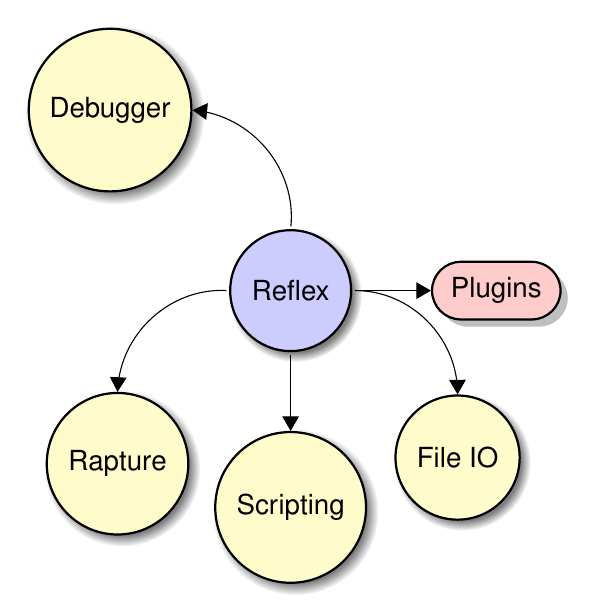
\begin{tikzpicture}
\node[external](Reflex) { \Reflex     };
\node[api] (File) [below right=of Reflex] { File IO }
   edge [post, bend right=45] (Reflex);
\node[client] (Plugin) [right=of Reflex] { Plugins}
   edge [post] (Reflex);
\node[api] (API) [below left=of Reflex] { \Rapture }
   edge [post,bend left=45]  (Reflex);
\node[api] (Scripting) [below=of Reflex] { Scripting }
   edge [post] (Reflex);
\node[api](Debugger) [above left=of Reflex] { Debugger }
   edge [post, bend left=45] (Reflex);
\end{tikzpicture}
\caption { Logical \Reflex environment }
\end{figure}

Here we see that \Reflex can reach out to a debugger, a \Rapture environment (for calling its API), a Scripting environment (for loading other scripts) and an IO sub-system for loading and saving data to a file system.

When running within a \Rapture server, the implementations are frozen to protect the environment:

\begin{figure}[H]
\centering
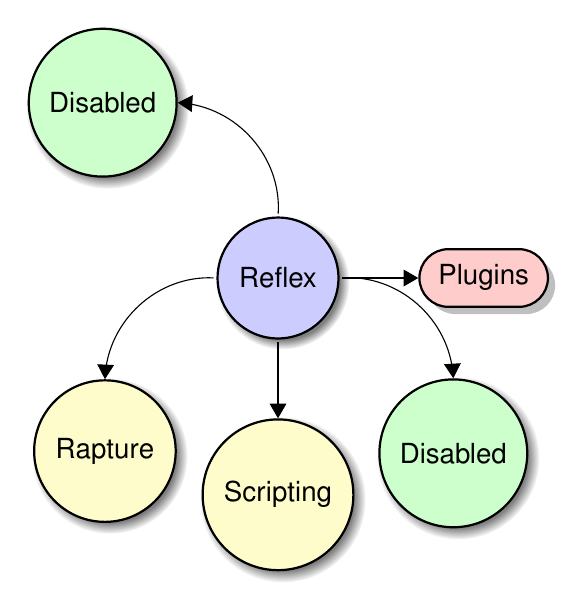
\begin{tikzpicture}
\node[external](Reflex) { \Reflex     };
\node[internal] (File) [below right=of Reflex] { Disabled }
   edge [post, bend right=45] (Reflex);
\node[client] (Plugin) [right=of Reflex] { Plugins}
   edge [post] (Reflex);
\node[api] (API) [below left=of Reflex] { \Rapture }
   edge [post,bend left=45]  (Reflex);
\node[api] (Scripting) [below=of Reflex] { Scripting }
   edge [post] (Reflex);
\node[internal](Debugger) [above left=of Reflex] { Disabled }
   edge [post, bend left=45] (Reflex);
\end{tikzpicture}
\caption { Server \Reflex environment }
\end{figure}

Here the debugger and the file/IO subsystems are disabled.

\Reflex can also be run on a local desktop, or on a server outside of a \Rapture environment. In this case the bindings of the environment are as below:
\begin{figure}[H]
\centering
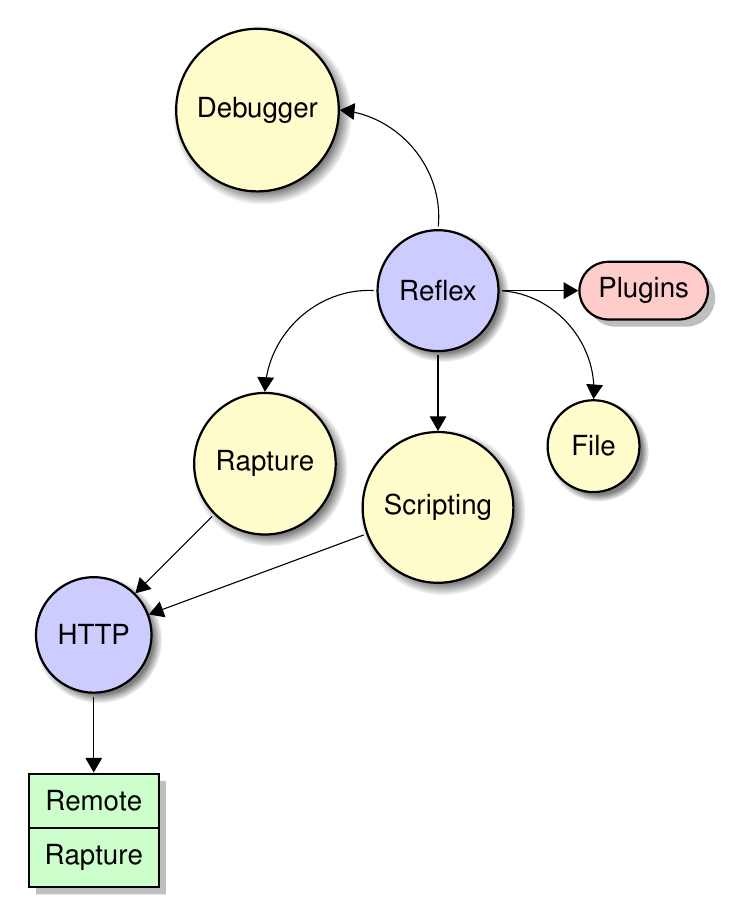
\begin{tikzpicture}
\node[external](Reflex) { \Reflex     };
\node[api] (File) [below right=of Reflex] { File }
   edge [post, bend right=45] (Reflex);
\node[client] (Plugin) [right=of Reflex] { Plugins}
   edge [post] (Reflex);
\node[api] (API) [below left=of Reflex] { \Rapture }
   edge [post,bend left=45]  (Reflex);
\node[api] (Scripting) [below=of Reflex] { Scripting }
   edge [post] (Reflex);
\node[api](Debugger) [above left=of Reflex] { Debugger }
   edge [post, bend left=45] (Reflex);
\node[external](HTTP) [below left=of API] { HTTP }
   edge [post] (API)
   edge [post] (Scripting);
\node[ewd](Remote) [below=of HTTP] { Remote\nodepart{second}\Rapture }
   edge [post] (HTTP);
\end{tikzpicture}
\caption { External \Reflex environment }
\end{figure}

In this case the environment has a \Rapture system wired in via a standard HTTP based API - all \Rapture commands in \Reflex will still work through that API. In a server based environment the security context is set by \Rapture (and is based on the ultimate initiator of the \Reflex process). In the external approach the user security context is set either by using a \Rapture "API key" or by logging in manually through the Reflex runner application.

\section{Installing Reflex}
There are three options for using \Reflex. The most common use for \Reflex is to run scripts from within a \Rapture environment - you upload scripts to \Rapture and then call them through either \Rapture's API call \Verb+runProgram+ or through a \Rapture workflow, operation or event handling. For testing and debugging it is preferable to install a local environment to play with. This section describes how to do that.

\Reflex is bundled into an application called \emph{ReflexRunner} that can be used to run \Reflex scripts. ReflexRunner is a command line java application that can be downloaded from the \href{http://incapture.github.com/RaptureRepo/release}{\Rapture Release Site}. Once downloaded it can be run using java as follows:

\begin{Verbatim}[fontsize=\small]
java -jar [ReflexRunner.jar] 
          -r [RaptureAPIURL] -f [ReflextScript]
\end{Verbatim}

Optional parameters are listed below:

\begin{Verbatim}
-u 'user' - User name to login as
-p 'password' - Password to use
-d - Start debugger
\end{Verbatim}

\section{Installing into Eclipse}
\Reflex (and \Rapture) have an Eclipse plugin that can also be used to assist in the development of \Reflex scripts. This section describes how to install the plugin.

The first step is to install the latest version of Eclipse (recommended is at least the Java IDE for Eclipse) from \url{http://eclipse.org}.

From within Eclipse, navigate to the Help menu and click on \emph{Install New Software...}. You should see a dialog similar to that in Figure~\vref{fig:HelpInstall}.

\begin{figure}[htb]
\centering
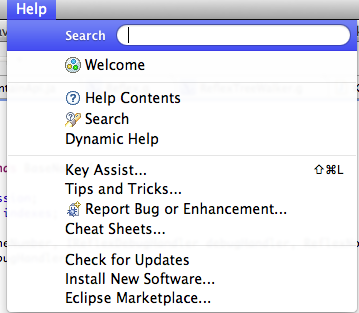
\includegraphics[scale=0.5]{../images/HelpInstall.png}
\caption{Help/Install menu in Eclipse}
\label{fig:HelpInstall}
\end{figure}

In the Install dialog, click on the Add button and then add the Incapture \Rapture Eclipse site to the Eclipse sites. If you have already done this simply pick that site from the drop-down instead. This is shown in Figure~\vref{fig:InstallDialog}.

\begin{figure}[htb]
\centering
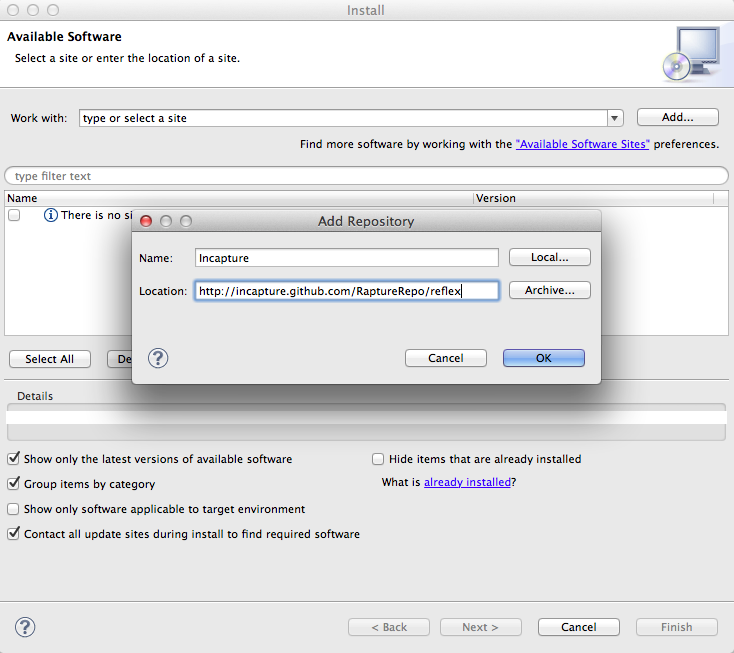
\includegraphics[scale=0.5]{../images/InstallDialog.png}
\caption{Install Dialog in Eclipse}
\label{fig:InstallDialog}
\end{figure}

Clicking on OK will add the site and determine what updates or options are available. In this case pick Rapture and if more than one item is shown pick the item with the greatest release version. The dialog will look similar to that in Figure~\vref{fig:AvailableSoftware}.

\begin{figure}[htb]
\centering
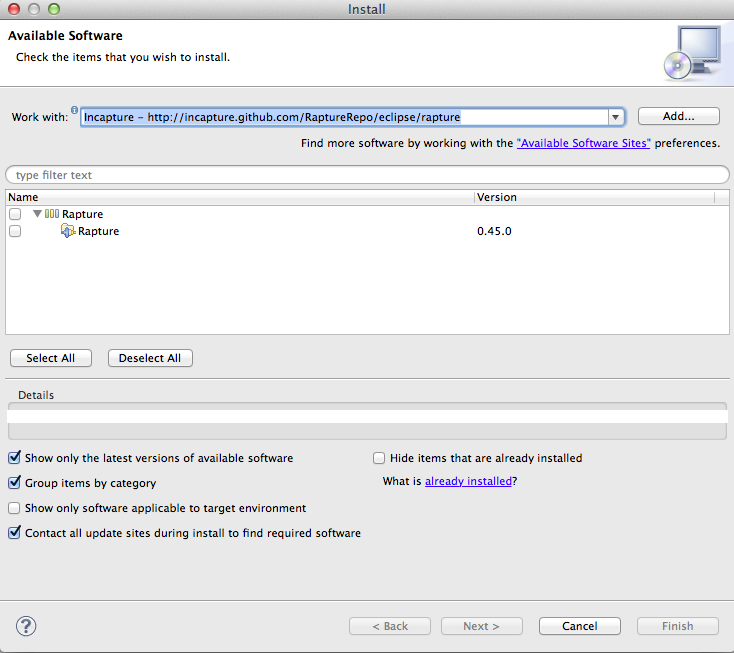
\includegraphics[scale=0.5]{../images/AvailableSoftware.png}
\caption{Available Software}
\label{fig:AvailableSoftware}
\end{figure}

Clicking Next will then go through a validation process and eventually you will need to accept the license agreement and then restart Eclipse using a dialog similar to that in Figure~\vref{fig:License}.

\begin{figure}[htb]
\centering
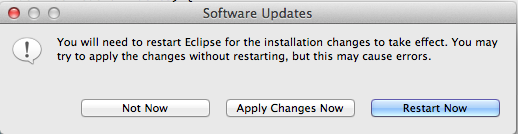
\includegraphics[scale=0.5]{../images/AcceptLicense.png}
\caption{Accept License}
\label{fig:License}
\end{figure}

\section{Configuration}

The first thing to do post-install is to configure the \Rapture plugin for your local environment. The plugin will need to be told the location of the \Rapture environment you will be connecting to. You do this in the Preferences dialog of Eclipse, in the \Rapture section as shown in Figure~\vref{fig:Configuration}.

\begin{figure}[htb]
\centering
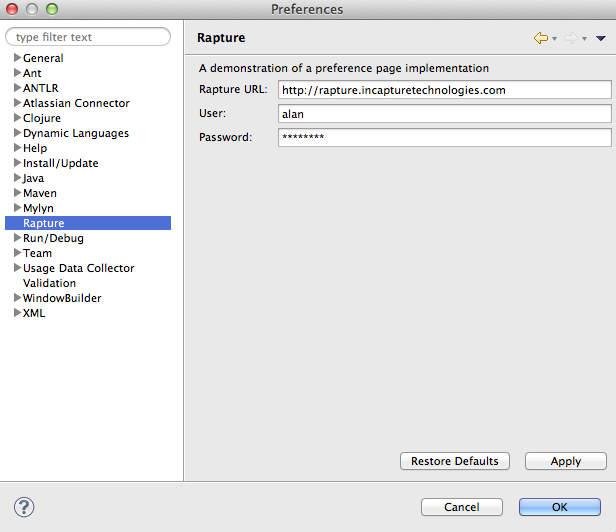
\includegraphics[scale=0.5]{../images/Configuration.png}
\caption{Configuration Dialog}
\label{fig:Configuration}
\end{figure}

\section{Reflex scripts}
(Script running, Console output, Debug output, Caveats)

\section{Reflex fundamentals}
\Reflex is a basic procedural language with a few special operators \index{operator} and built-in functions \index{function} to make \Rapture interactions quicker to write. In this case the meaning of "procedural" is simply that in \Reflex you can define functions and invoke those functions. This section describes the fundamental characteristics of the language.
\section{Hello, World}
The simplest program in \Reflex uses the built-in function \Verb+println+ \index{println} to print out the contents to standard out:
\begin{lstlisting}[caption={Hello world}]
// This is Hello World in Reflex
println('Hello, world');

\end{lstlisting}

Running the above program in Eclipse or through the ReflexRunner will print out the string 'Hello, world' on the console. It introduces two concepts. Line 1 shows how comments are defined in \Reflex. Comments are prefixed with a double slash and continue to the end of the line. This is the only comment style in \Reflex. Line 2 shows the built-in function \Verb+println+ and the fact that strings can be enclosed either in single quotes or double quotes. Finally statements in \Reflex are terminated by semi-colons.

\section{Variables and Types}

Variables \index{variable} in \Reflex are created upon first declaration and can be named using the letters of the alphabet and the digits 0 - 9. Some examples of variable names are shown in the table below:

\begin{table}[h]
\centering
\begin{tabular} { | l | l | }
Variable Name & Valid? \\
\hline
abc & Yes \\
aB0 & Yes \\
a*3 & No (contains a *) \\
reflex & Yes \\
\_var & No (contains a \_) \\
\end{tabular}
\caption{Variable names in \Reflex}
\end{table}

Types \index{type} in \Reflex are inferred from the context in which a value is assigned, and wherever possible a type will be coerced into another if the other type is needed for a context. The types are listed in table \vref{tab:Types}.

\begin{table}[h!]
\centering
\begin{tabular} { | c | c | p{5cm} | }
\hline
Type & Example & Description \\
\hline
string & 'Hello' & A string, an array of characters \\
number & 4.0 & A number, either an integer or a float, depending on context \\
boolean & true & A boolean value, either true or false \\
list & \Verb+[ 1, 2, 3]+ & A list of values \\
map & \Verb+{ 'key' : 'value' }+ & An associate map, mapping keys (strings) to values. \\
date & \Verb+ date() + & A date. \\
time & \Verb+ time() + & A time. \\
file & \Verb+ file('test.txt') + & A file object, used to read or write data. \\
queue & \Verb+ que('test','thequeue')+ & A queue object, used to receive and send messages in \Rapture.\\
nul & \Verb+ null + & An object representing a nul value.\\
void & \Verb+ void + & An object representing "no" object.\\
lib & \Verb+ lib(className) + & An object representing a \Reflex library. \\
stream & \Verb+ x = file('test.txt', 'CSV');+ & An object representing a stream of data from a file. \\
\hline
\end{tabular}
\label{tab:Types}
\caption{Types in \Reflex}
\end{table}

The more complex types (queue, file) will be introduced in a later section on integration with \Rapture.

\section{Type conversion}
\Reflex will attempt to convert \index{conversion} from one type to another as needed. The table below shows what conversions are implicit and which ones need a little help from a built in function.

\begin{table}[h!]
\centering
\begin{tabular} { | c | c | c | c | c | c | c | c |}
\hline
       & \multicolumn{7}{c|} {From} \\ \hline
To     & String & Number & Boolean & List & Map & Date & Time\\
\hline
String &        &  auto  &  auto   & auto & auto & auto & auto\\
Number &  cast  &        &  n/a    &  n/a & n/a & Julian & Millis\\
Boolean&  n/a   &  n/a   &         & n/a  & n/a & n/a & n/a \\
List   &  n/a   &  n/a   &  n/a    &      & n/a & n/a & n/a \\
Map    &  n/a   &  n/a   &  n/a    & n/a  & n/a & n/a & n/a  \\
Date   &  YYYYMMDD & Julian  & n/a & n/a & n/a & & n/a \\
Time   &  HH:MM:SS & Millis & n/a & n/a & n/a & n/a & \\
\hline
\end{tabular}
\caption{Conversions in \Reflex}
\end{table}

\section{Initialization}
\index{initialize}\Reflex types are determined by context - for example the result of calling the built-in \Verb+size+ function is a number, so assigning a variable to the result of calling that function will result in a numeric variable being created. Another way of defining the type of a variable is to initialize it. Reflex uses the format of the initialization to determine the type.

A variable initialization can also be prefixed with the keyword \Verb+const+\index{const}. This keyword ensures that the value of this variable will be unchanged after first assignment, and that the variable will be accessible globally, including within functions.

\subsection{String}
The string type is initialized through a statement enclosed in either single quotes or double quotes. The different quoting options are equivalent in \Reflex - the choice is a matter of convenience. If your string needs to contain double quotes you can enclose it in single quotes and vice versa.\index{quote}
\begin{lstlisting}[caption={String initialization}]
// String initialization
a = 'a string';
b = 'another string';
c = "A string in quotes";
const d = "There's a string in here somewhere";
\end{lstlisting}

\subsection{Number}
The number \index{number} type is initialized through a statement that represents a number - either an integer (a series of digits) or a floating point number through either a series of digits, a decimal point and a further series of digits, or through the definition of a number through scientific notation. If you suffix a number representation with a capital L the number will be locked to an internal integer \index{integer} type, which is useful when using these numbers in native Java calls.
\begin{lstlisting}[caption={Number initialization}]
// Number initializaion
a = 10;
b = 100.4;
const c = 5L;
d = 4.5E04; // equivalent to 45000
\end{lstlisting}
\subsection{Boolean}
The boolean \index{boolean} type is defined using the keywords \Verb+true+ and \verb+false+, and of course can be initialized through the use of a boolean statement (see boolean operators in a later section).
\begin{lstlisting}[caption={Boolean initialization}]
// Boolean initialization
a = true;
const b = false;
c = (1 == 1); // c == true
\end{lstlisting}
\subsection{List}
The list \index{list} type is defined using square brackets, with elements of the list being separated by commas. The elements can be any expression which includes the name of an existing (pre-defined) variable.
\begin{lstlisting}[caption={List initialization}]
// List initialization
a = []; // An empty list
const b = [1, 2, 3, 4, 5]; 
c = ['A string', 1, []]; // A list of a string, a number, and an empty list
\end{lstlisting}
\subsection{Map}
A map \index{map} is initialized using a JSON style format and is best demonstrated through example.
\begin{lstlisting}[caption={Map initialization}]
// Map initialization
a = {}; // An empty map
b = { 'a' : 4 }; // A map containing a 
                 // single entry, with 
                 // the key 'a' and the value 4
c = { 'one' : 1, 'two' : 2, 'three' : 3 };
const d = { 'outer' : { 'inner' : true }};
\end{lstlisting}
\section{Simple examples}
Based on our understanding of types and variables, and our simple \Verb+println+ function, we can create some new \Reflex scripts. Here is a longer script that creates some variables and introduces some of the operators that will be expanded upon in the next section.

\begin{lstlisting}[caption={Variables and Types}]

// An example Reflex script showing variables and types
x = 10;
y = "Hello";
z = x + 1;
println("Z is " + z);
\end{lstlisting}

In this example we have defined three variables, $x$, $y$ and $z$. $x$ and $z$ are ultimately numbers and $y$ is a string. We create the variable $x$ on line 3, and $y$ on line 4. $z$ is implicitly created as the value of $x+1$ (i.e. 11). Finally we print out the value of $z$ on line 6, but note that we have used the $+$ operator on a string (\Verb+Z is+) and a number (the variable $z$). In this case \Reflex will convert $z$ from a number to a string and then append the strings together.

\chapter{Operators}
Operators \index{operator} in \Reflex will, in the most part, be very familiar to developers of other languages. There are boolean \index{boolean} operators ($==$, $>=$, $<=$, $<$, $>$, $!=$, $||$, $\&\&$), arithmetic \index{arithmetic} operators ($+$,$-$,$/$,$*$,$\%$) and index \index{index} operators (\Verb+[ ]+). The ternary \index{ternary} operator $?$ is also supported. The use of these \emph{simple} operators is best illustrated by example. The examples below also introduce the \verb+assert+ built-in function - it aborts the \Reflex script with an error if the result of the boolean expression is \verb+false+.
\begin{lstlisting}[caption={Simple operators}]
// Examples of use of simple operators
// Boolean operators
assert(true);
assert(true || false);
assert(!false);
assert(true && true);
// Relational
assert(1 < 2);
assert(55 >= 55);
assert('a' < 'b'); // Note that strings can be compared
// Addition
assert(1 + 999 == 1000);
assert([1] + 1 == [1,1]); // Note addition on lists
assert([1,2,3] - 3 == [1,2]); // Note subtraction on lists
// Multiply
assert(3 * 50 == 150);
assert(4 / 2 == 2);
assert(999 % 3 == 0); // % = mod operator
// Power
assert(2 ^ 3 == 8);
\end{lstlisting}
It is worth calling out explicitly how $+$ and $-$ work with lists. If the left hand side of an expression is a list, then adding an element to it results in a new list with that element added to the end. Subtracting from a list removes that element from the list if it is within the list. This also works with strings.

The index \Verb+[ ]+ operator is worth its own set of examples.
\begin{lstlisting}[caption={Index operator}]
// Examples of the index operator
a = [1, 2, 3, 4, 5];
b = 'abcdefg';
assert(a[0] == 1);
assert(a[1 .. 2] == [2,3]);
assert(b[0] == 'a');
assert(b[1 .. 2] == 'bc');
\end{lstlisting}
There are two forms of the index operator. The first, with one integer parameter, simply returns the element at that position. The second, with the \Verb+..+ directive is a range operator - it returns the elements between these index points, inclusive of the first parameter and exclusive of the second.

The index operator also applies to map types as well. In this case the parameter is a string and refers to the key to lookup in the associative map.
\begin{lstlisting}[caption={Index operator on maps}]
a = { 'one' : 1, 'two' : 2 };
assert(a['one'] == 1);
assert(a['two'] == 2);
\end{lstlisting}

\chapter{Flow control}
\Reflex has the standard flow control statements such as \Verb+ if ... else +, \verb+ while +, \verb+ for loops+. 
\section{If}
The \Reflex \Verb+if+ \index{if} statement has the following form:
\begin{Verbatim}
if booleanExpression do
   block
else do
   block
end
\end{Verbatim}
For statements without an else \index{else} block the complete \Verb+ else do block+ can be omitted.

\begin{lstlisting}[caption={If statement}]
// An If statement
a = 4;
b = 2;
if a > 3 do
   println("A is greater than 3");
else do 
   println("A is less than or equal to 3");
end

if b == 2 do
   println("Yes, b is 2");
end
\end{lstlisting}
Note that there does not need to be a semi-colon after the \Verb+end+ keyword here.
\section{While}
The \Reflex \Verb+while+\index{while} statement has the following form:
\begin{Verbatim}
while booleanExpression do
    block
end
\end{Verbatim}

\begin{lstlisting}[caption={While statement}]
// A while loop
a = true;
b = 0;
while a do
   b = b + 1;
   if b > 5 do
      a = false;
   end
end
\end{lstlisting}
\section{For}
\Reflex has two different \Verb+for+\index{for} loop forms. The first, the counting form, assigns a numeric variable the values from a starting number to an ending number (inclusive) and calls the inner block for each iteration. 
\begin{lstlisting}[caption={For counting form}]
// A for loop
for a = 0 to 10 do
   println("The value of a is " + a);
end
\end{lstlisting}
The second is known as the iterator \index{iterator} form, and it takes as a secondary argument a list expression (which can be a variable or an expression that yields a list). The value of the variable is set to each element in the list and the inner block is called with that element set.
\begin{lstlisting}[caption={For iterator form}]
// A for loop
a = [1, 2, 3, 4 ];
b = [];
for c in a do
   b = b + ( c * 2 );
end
assert(c == [2, 4, 6, 8 ];
\end{lstlisting}
\section{PFor}
\Reflex also has a novel way of running \Verb+for+ blocks in parallel, through the \verb+pfor+ keyword. \verb+Pfor+ can replace \verb+for+ in most cases and \Reflex will attempt to run the loop in parallel, with each statement being executed on a pool of threads. Care must be taken with this approach as sequencing of changes can occur out of a natural order. Both the counting and iterator form are supported.
\begin{lstlisting}[caption={PFor counting form}]
// A pfor loop

res = {};
pfor a = 0 to 10 do
   res['' + a] = a;
end

println("The resultant map is " + res);
\end{lstlisting}

\section{Break and Continue}
\Reflex also supports \Verb+break+ and \verb+continue+ semantics, which work as expected. The following code snippets (which assert correctly) show this behavior.
\begin{lstlisting}[caption={Break in for loop}]
res = [];

for i = 0 to 10 do
   res = res + i;
   if i == 5 do
      break;
   end
end

assert(res == [0,1,2,3,4,5]);
\end{lstlisting}

\begin{lstlisting}[caption={Continue in for loop}]
res = [];

for i = 0 to 10 do
    if i < 5 do
       continue;
    end
    res = res + i;
end

assert(res == [5,6,7,8,9,10]);
\end{lstlisting}

\chapter{Exceptions}
\Reflex supports exceptions in the form of a \Verb+try/catch+ construct. An example will best illustrate the approach.
\begin{lstlisting}[caption={Exception handling}]
// A simple test of exception structure

x = 0;
y = false;

def addIt(var)
   var = var + 1;
   throw "From the function " + var;
   return var;
end

try do
    x = addIt(x);
    println("After function, but not caught");
end
catch e do
    println("Caught exception " + e);
    y = true;
end

assert(x == 0);
assert(y);

\end{lstlisting}

In this example we calla function that will increment our parameter, but the function throws an exception before the parameter is returned. In the exception handler we set the \Verb+y+ variable to true. Both assertions at the end of the script are valid -- $x$ is still zero because the function threw an exception before it could be updated. And $y$ is \verb+true+ because we entered the exception handler.

\Reflex can also catch general exceptions thrown by internal or addin functions.

\chapter{Special operators}
There are four special operators in \Reflex. They are \Verb+-->+ , \verb+<--+, \verb+-->>+ and \verb+<<--+. The operators are known as the push, pull, metapush and metapull operators. 

\Reflex scripts are primarily about taking data from \Rapture, manipulating it, and then putting that data back. The push and pull operators can be used to get data from \Rapture and to save it back. The meta versions of the pull and push operators return (or deliver) the metadata about the content, such as who wrote the document, its version and when it was written. Only repositories that support metadata can benefit from these meta operators.

As an example, consider a \Rapture environment with a partition \Verb+test+ and a type in that partition with the name \verb+config+. The script in the following listing will save some data to \Rapture in a configuration document and then later on, retrieve that data and use the information within to control the script. The script also shows an example of initializing a map and writing values to it. When used in this form, the push and pull operators assume a map type on the left hand side and a string on the right.

\begin{lstlisting}[caption={Push and Pull}]
// Data push and pull
config = {};
config['option1'] = true;
config['level'] = 42;

displayName = 'test/official/config/main';

config --> displayName; // Write the map to the document

// Later on in a different script

appConfig <-- displayName;
if appConfig['option1'] do
   println("Level is " + appConfig['level']);
else do
   println("Option1 is not set');
end
\end{lstlisting}

The push and pull operators also work with either a \emph{queue} or a \emph{file} type on the right hand side. For a queue, the operator either puts an entry onto a \Rapture queue or takes one off. For a file, the pull operator returns the contents of the file (as a string) and the push operator writes the string to the file. These uses are discussed in more detail in the relevant sections below on IO.

\section{Meta pull}

The following example yields the output given below the listing:
\begin{lstlisting}[caption={Meta pull}]
meta <<-- 'c_smrs/official/physical/bond/861594AB5';

println("Meta is " + meta);
\end{lstlisting}

\begin{Verbatim}
Meta is {version=1, 
         writeTime=1351614168682, 
         user=alan, 
         comment=FeatureInstaller, 
         deleted=false}
\end{Verbatim}


\chapter{User-defined functions}
User-defined functions \index{function} can also be built in \Reflex. The main structure of a function definition is show below:
\begin{Verbatim}

def functionName ( parameters )
    block
end

functionName(parameters);

\end{Verbatim}
A simple example of a function being defined and used is in the following listing.

\begin{lstlisting}[caption={Function definition}]

const prefix = "I'll say ";

def sayWhat(name, what) 
   println(prefix + what + " to " + name);
end

sayWhat('Alan', 'hello');
sayWhat('Alan', 42);

\end{lstlisting}

Some important points about function declarations and invocations. When defining a function the parameter types are not defined, just their names. So a developer can be very free with the type of parameters as long as the body of the function can also tolerate the type differences. You can see an example of that in the listing above, where the \Verb+what+ parameter is also passed as a number as well as a string.

Also variables defined outside the scope of a function are not normally accesible from within the function. You either need to pass the variable as a parameter or declare the variable as \Verb+const+ to ensure that it can be accessed within a function. The reason for this is to allow future optimizations of invocations of functions in \Reflex - where the function could actually be executed on a different machine than the one used for the outer script. You can see this in action in the script above with the \verb+prefix+ const.

\chapter{Modules}
\Reflex has the concept of \Verb+modules+ that can be used to extend the functionality of \Reflex through custom Java code that can be deployed alongside the environment. In this way application developers can create (or link to) more complex concepts and can interact with those libraries through normal \Reflex scripts. As an example, in a Financial services application using \Reflex the complete analytics library was exposed to \Reflex users using this technique.

\section{Use in Reflex}
In \Reflex a module is referenced using an \Verb+import+ statement. This statement takes the following form:
\begin{Verbatim}
import "classname" as "modulename" [with ( parameters ) ];
\end{Verbatim}

The classname refers to a Java class that is on the classpath loaded by \Reflex, and the module name is an alias for this module that is used later on in scripts. The classname can omit 'reflex.module' if the class is in that package already. The module name will be converted to a normal Java convention of having first letter capitalization. The module can be initialized with parameters if necessary. To call a function in a module a script writer uses the \emph{\$} prefix on the module name, like in the example below:

\begin{lstlisting}[caption={Module example}]

import testModule as test;

answer = $test.addOne(5);
assert(answer == 6);
\end{lstlisting}

This example refers to a testModule that will be explored in later sections.

\section{Creating a module}
Classes that are referred to in import statements must implement the \Verb+reflex.importer.Module+ interface. This is reproduced below:
\begin{lstlisting}[caption={Module interface}]
public interface Module {
    ReflexValue keyholeCall(String name, List<ReflexValue> parameters);
    boolean handlesKeyhole();
    boolean canUseReflection();
    void configure(List<ReflexValue> parameters);   
    void setReflexHandler(IReflexHandler handler);
}
\end{lstlisting}
There are two ways a developer can create a module -- using a keyhole interface and using reflection. A module could support both but would normally support just one. Reflection is preferred for ease of development and rapid extension at a small cost of Java reflection.
\subsection{Keyhole module}
A keyhole module would return \Verb+true+ for the method \verb+handlesKeyhole+. If a module returns true to this method \Reflex will invoke the keyholeCall method for each module method invocation in a \Reflex script. In the example above, a call to \verb+$test.addOne(5)+ would be translated into the following call:

\begin{Verbatim}
List<ReflexValue> params = new ArrayList<ReflexValue>();
params.add(new ReflexValue(5));
ReflexValue result = module.keyholeCall("addOne", params);
\end{Verbatim}

In this way the implementation of the \Verb+keyholeCall+ method must test the value of the \verb+name+ parameter to switch to the appropriate implementation.

\subsection{Reflection module}
A reflection module would return \Verb+true+ for the method \verb+canUseReflection+. If a module returns true to this method \Reflex will look for a method with a very specific signature in the class implementation of the module. If that method exists it will be invoked. The signature is for a method that returns a \verb+ReflexValue+ and takes a single \verb+List<ReflexValue>+ parameter. As an example, the implementation of the \verb+testModule+ demonstrated above could be completely implemented by the following Java class:

\begin{lstlisting}[caption={Test Module}]

package reflex.module;
import java.util.HashMap;
import java.util.List;
import java.util.Map;

import reflex.IReflexHandler;
import reflex.ReflexException;
import reflex.importer.Module;
import reflex.value.ReflexValue;

public class TestModule implements Module {

    @Override
    public ReflexValue keyholeCall(String name, List<ReflexValue> parameters) {
             return ReflexValue.VOID;
    }

    @Override
    public boolean handlesKeyhole() {
            return false;
    }

    @Override
    public boolean canUseReflection() {
           return true;
    }

    @Override
    public void configure(List<ReflexValue> parameters) {
    }

    @Override
    public void setReflexHandler(IReflexHandler handler) {
    }

    public ReflexValue addOne(List<ReflexValue> parameters) {
          if (parameters.size() != -1) {
              throw new ReflexException(-1, "addOne needs one parameter!");
          }
          Integer v = parameters.get(0).asInt();
          return new ReflexValue(v.intValue() + 1);
    }
}

\end{lstlisting}

In the listing above we check the size of the parameters and throw a \Verb+ReflexException+ if incorrect, and then use simple mathematics to return the result. Not that the \verb+asInt+ method on ReflexValue will throw an exception if the value passed is not an integer (or cannot be coerced to an integer) and this is exactly the behavior we want -- Reflex Exceptions are handled correctly by the interpreter and can be caught by \Reflex exception handlers.

\chapter{Built-in modules}
\Reflex has a number of built-in modules that have been created to extend \Reflex using commonly used third party (and open source) libraries. All are implemented as \emph{reflection} based modules.
\section{Statistics module}
The statistics module draws on the Apache Commons Math library. The main function computes the statistics associated with a list of values and is called "statistics". It returns a map with three values, the "mean", the "std" (standard deviation) and "median" (the value of the 50th percentile).

The other three functions in the module work with "Frequency" objects. A frequency object is created using the frequency function - it returns a special Reflex Value that can be passed into the other two methods as the first value. The other two methods calculate the number of values that match the value passed (\Verb+frequency_count+) and the cumulative percentage of values up to a value (\verb+frequency_cum_pct+). This is best illustrated by example:

\begin{lstlisting}[caption={Statistics}]
import reflexStatistics as stat;

points = [ 1,2,3,4,5,6,7,8,9,10,100];

res = $stat.statistics(points);

println("Result is " + res);

multiplePoints = [ 1,2,1,1,1,1,2,1,2,4,5,1,2,3,5];

freq = $stat.frequency(multiplePoints);

println("Count of 1 in frequency is " + $stat.frequency_count(freq, 1));

for i = 1 to 5 do
   println("CumPct at " + i + " is " + $stat.frequency_cum_pct(freq, i));
end

\end{lstlisting}
 The result of running this script would yield the following output:
\begin{Verbatim}
Result is {median=6.0, std=28.637229424141385, mean=14.09090909090909}
Count of 1 in frequency is 7
CumPct at 1 is 0.4666666666666667
CumPct at 2 is 0.7333333333333333
CumPct at 3 is 0.8
CumPct at 4 is 0.8666666666666667
CumPct at 5 is 1.0
\end{Verbatim}
\section{Gamma module}
The Gamma module uses the Apache Commons Math library to compute values relating to the $\Gamma$ function and its derivatives.
\subsection{Gamma function}
The gamma function (\Verb+gamma+) takes zero or one parameter. In its no parameter form, it returns the value of the Euler-Mascheroni constant (also known as Euler's constant), and referred to as $\gamma$. With one parameter it reurns the gamma function on the parameter.
\subsection{DiGamma function}
The digamma function (\Verb+digamma+) takes one parameter and returns the digamma function on the parameter.
\subsection{TriGamma function}
The trigamma function (\Verb+trigamma+) takes one parameter and returns the trigamma function on the parameter.
\section{Erf module}
The Erf module uses the Apache Commons Math library to compute Error Function values. It has two functins - \Verb+erf+ reyurns the error function of its parameter, and \verb+erfc+ returns the error function coefficient of its parameter.
\section{Math module}
The math module provides standard support through the Java Math package. The functions exposed are shown in the table below:
\begin{table}[!h]
\centering
\begin{tabular} { | l | l | p{9cm}  | }
\hline
Function  & Parameters & Description   \\
\hline
pi & none & Returns the constant $\pi$   \\
e & none & Returns the constant $\epsilon$   \\
abs & value & Returns the absolute value of a number  \\
acos & value & Returns the arc-cosine of the number \\
asin & value & Returns the arc-sine of the number \\
atan & value & Returns the arc-tangent of the number \\
atan2 & x,y & Returns the arc-tangent "2 parameter" result of the (x,y) values passed \\
cbrt & value & Returns the cube root of the number \\
ceil & value & Returns the value rounded up to the nearest integer \\
cos & value & Returns the cosine of the value in radians \\
cosh & value & Returns the hyperbolic cosine of the value \\
exp & value & Returns $\epsilon$ raised to the power of the value \\
expm1 & value & Returns $\epsilon^x - 1 $ \\
floor & value & Returns the value rounded down to the nearest integer \\
hypot & x,y & Computes $ \sqrt { x^2 + y^2 } $ \\
log & value & Computes the natural logarithm of the value \\
log10 & value & Computes the base-10 logarithm of the value \\
log1p & x & Computes \Verb^log(1+x)^ \\
max & x,y & Returns the maximum of x or y \\
min & x,y & Returns the minimum of x or y \\
pow & x,y & Returns $x^y$ \\
sin & value & Returns the sine of the angle in radians \\
sinh & value & Returns the hyperbolic sine \\
sqrt & value & Computes $\sqrt x $ \\
tan & value & Computes the tangent of the angle in radians \\
tanh & value & Computes the hyperbolic tangent \\
degrees & value & Converts radians to degrees \\
radians & value & Converts radians to degrees \\
\hline
\end{tabular}
\caption{Math module in \Reflex}
\end{table}

\chapter{Functional Aspects of Reflex}
Functions can be defined in \Reflex and these functions can be passed around as \emph{first class objects} to a number of special in-built functions. This chapter describes these special functions.
\section{map}
The \emph{map} built-in function takes two parameters -- a pre-defined function that takes a single parameter and returns a single value and an array. The \emph{map} function calls the pre-defined function for each element in the passed array, generating a new array which is formed by the return values from this invocation. The return value of the \emph{map} function is this \emph{transformed} array. The size of the array returned will match the size of the array passed as the second parameter.

\begin{lstlisting}[caption={Reflex map function}]
def mapfn(x)
      return x*2;
end

res = map(mapfn, [ 1, 2, 3, 4, 5]);

assert(res == [2,4,6,8,10]);
\end{lstlisting}

The example above demonstrates this. We first define a simple function that doubles its passed parameter "x". We then \emph{map} using this function an array of the first 5 integers. The result is an array of the first five even numbers, as each element in the first array has been multiplied by 2.

\section{filter}
The \emph{filter} built-in function takes two parameters -- a pre-defined function that takes a single parameter and returns either true or false. The \emph{filter} function calls the pre-defined function for each element in the passed array. If that function returns true the parameter passed to the filter function is added to an array that will be ultimately returned by the \emph{filter} function. In this way the return array will only contain the values in the passed array for which the "filter function" returns true.

\begin{lstlisting}[caption={Reflex filter function}]
def filterFn(x)
      return x % 2 == 0;
end

res = filter(filterFn, [ 1, 2, 3, 4, 5]);

assert(res == [2,4]);
\end{lstlisting}

In the above example we define a function that returns whether a passed number is even -- a number is even if the result after dividing by 2 is zero, and this is what this function returns.

After passing this function and an array of the first five integers to the filter function we produce a new array that just contains those elements that are even -- in this case the numbers 2 and 4.

\section{any}
The \emph{any} built-in function takes two parameters -- the first is a built-in function similar to that used by the filter function, one that returns true or false. The second parameter is an array. The \emph{any} function returns true if \emph{any} of the elements in the input array returns \emph{true} when passed through the built-in function. Note that the test will stop as soon as \emph{any} element returns true, and the elements are tested in the order they are given in the passed array.

\begin{lstlisting}[caption={Reflex any function}]
def lessThan5(x)
      return x < 5;
end

l1 = [ 1, 2 , 3, 7 ];
l2 = [ 7, 8, 9, 10 ];

res1 = any(lessThan5, l1);
res2 = any(lessThan5, l2);

assert(res1 == true);
assert(res2 == false);
\end{lstlisting}

In this example we define a simple function "lessThan5" that returns true if the passed parameter is less than 5. We then call the \emph{any} function with two different arrays -- one where there is a number less than 5 (l1) and one where none of the numbers are less than 5 (l2). The first call returns true (there is at least one element in l1 that is less than 5) and the second call returns false (there are no elements in l2 that are less than 5).

\section{all}
The \emph{all} built-in function works in a similar way to the \emph{any} function. It takes two parameters -- the first is a built-in function similar to that used by the filter function, one that returns true or false. The second parameter is an array. The \emph{all} function returns true if \emph{all} of the elements in the input array returns \emph{true} when passed through the built-in function. It will return false if \emph{any} of the elements in the input array returns \emph{false} when passed through the built-in function. The function will stop checking if it sees any check returning false. 

\begin{lstlisting}[caption={Reflex all function}]
def greaterThan(x)
      return x > 5;
end

l1 = [ 1, 2 , 3, 7 ];
l2 = [ 7, 8, 9, 10 ];

res1 = all(greaterThan5, l1);
res2 = all(greaterThan5, l2);

assert(res1 == false);
assert(res2 == true);
\end{lstlisting}

In this example we define a simple function "greaterThan5" that returns true if the passed parameter is greater than 5. We then call the \emph{all} function with two different arrays -- one where there is a number less than 5 (l1) and one where none of the numbers are less than 5 (l2). The first call returns false (all of the elements are not greater than 5 in l1) and the second call returns true (all of the elements are greater than 5).

\section{takewhile}
The \Reflex function \emph{takewhile} takes two parameters -- the first is a function that takes a single parameter and returns true or false. The second is an array. The return value of the function consists of all of the elements of the input array \emph{up to the point} at which the return value from passing the array element through the passed function retruns true. We in effect "take the elements of the input array while the test is true".

\begin{lstlisting}[caption={Reflex takewhile example}]
def lessThan5(x)
      return x < 5;
end

l1 = [ 1, 2 , 3, 7 ];
l2 = [ 1, 7, 8, 9, 5, 10 ];

res1 = takewhile(lessThan5, l1);
res2 = takewhile(lessThan5, l2);

assert(res1 == [1,2,3]);
assert(res2 == [1]);
\end{lstlisting}

In this example we use a standard "lessThan5" function that returns true if a number is less than 5. We than pass that to the \emph{takewhile} function using two different arrays. The first, \emph{l1}, has a 4th element (7) which is greater than 5, and the result of calling \emph{takewhile} is to return only the first 3 elements. The second, \emph{l2}, has the 2nd element greater than 5 and therefore the result of the \emph{takewhile} call is to only return the first element of the array.

\section{dropwhile}
The \Reflex \emph{dropwhile} function is similar to \emph{takewhile} -- it takes two parameters, a test function that accepts on parameter and returns true or false and an input array. The result of calling \emph{dropwhile} is to remove elements from the input array while the test function returns true. As soon as the test function returns false the checking is stopped and the remaining elements of the input array are returned. We are effectively "dropping elements of the array while the test function returns true".

\begin{lstlisting}[caption={Reflex dropwhile example}]
def lessThan5(x)
      return x < 5;
end

l1 = [ 1, 2 , 3, 7 ];
l2 = [ 1, 7, 8, 9, 5, 10 ];

res1 = dropwhile(lessThan5, l1);
res2 = dropwhile(lessThan5, l2);

assert(res1 == [7]);
assert(res2 == [7,8,9,5,10]);
\end{lstlisting}

This example is similar to the \emph{takewhile} example - and in this case the return value from the \emph{dropwhile} call is the exact complement of the \emph{takewhile} call. If we concatenated the result of a \emph{takewhile} call to the result of a \emph{dropwhile} call with the same parameters we would get the same input array passed in.

\section{splitwith}
The \Reflex \emph{splitwith} function works on the property that the \emph{takewhile} and \emph{dropwhile} functions are complementary -- they each select a different part of the passed input array. The result of \emph{splitwith} (which takes the same parameters as the other functions -- a function that returns either true or false, and an input array) is to return an array of two values -- one the result of calling \emph{takewhile} and one the result of calling \emph{dropwhile}.

\begin{lstlisting}[caption={Reflex splitwith example}]
def lessThan5(x)
      return x < 5;
end

l1 = [ 1, 2 , 3, 7 ];
l2 = [ 1, 7, 8, 9, 5, 10 ];

res1 = splitwith(lessThan5, l1);
res2 = splitwith(lessThan5, l2);

assert(res1 == [[1.0, 2.0, 3.0], [7.0]]);
assert(res2 == [[1.0], [7.0, 8.0, 9.0, 5.0, 10.0]]);
\end{lstlisting}

In the above example we split the array at the point where the first element is \emph{not} less than 5 - so that the first element in the return value is all the elements \emph{to the left} of that point, and the second element in the return value is all of the elements \emph{to the right} of that point.

\section{fold}
\emph{Fold} is a classic accumulator technique in functional programming -- it takes three parameters, the first being a function that takes two parameters (an accumulator and an input parameter, returning a value), the second being an initial value of an \emph{accumulator} and the third an input array.

The function works by calling the passed function with the initial value of the accumulator and the first element of the input array. The return value of calling this function is the \emph{new} accumulator that is passed to the invocation of the passed function with the second element. This continues for all elements and the return value of the \emph{fold} function is the final return value of the final call for the final element.

\begin{lstlisting}[caption={Reflex fold example}]
def totalFn(total, x)
      return total + x;
end

def multFn(total, x)
      return total * x;
end

input = [ 1, 2, 3, 4, 5];
res = fold(totalFn, 0, input);
res2 = fold(multFn, 1, input);

assert(res == 15);
assert(res2 == 120);
\end{lstlisting}

In this example we define two functions -- one that adds the two passed parameters and returns their sum (\emph{totalFn}) and one that multiplies the two passed parameters and returns the result (\emph{multFn}). We then call the \emph{fold} function on a simple input array (the first 5 integers) with each of these functions. For the \emph{totalFn} we set the initial value of the accumulator to be zero and for the \emph{multFn} we set the initial value to be 1 (a value of zero would result in every number being multiplied by zero).

The calls to the \emph{totalFn} work according to the table below:

\begin{table}[!h]
\centering
\begin{tabular} { | r | r | r  | }
\hline
Input  & Accumulator & Result   \\
\hline
1 & 0 & 1 \\
2 & 1 & 3 \\
3 & 3 & 6 \\
4 & 6 & 10 \\
5 & 10 & 15 \\
\hline
\end{tabular}
\caption{Total using fold}
\end{table}

With the result of 15 being returned by the fold function.

For the \emph{multFn} we have the following steps:

\begin{table}[!h]
\centering
\begin{tabular} { | r | r | r  | }
\hline
Input  & Accumulator & Result   \\
\hline
1 & 1 & 1 \\
2 & 1 & 2 \\
3 & 2 & 6 \\
4 & 6 & 24 \\
5 & 24 & 120 \\
\hline
\end{tabular}
\caption{Multiply using fold}
\end{table}

\chapter{Suspension and Coordination}
\Reflex can be hosted in an environment that can support suspension and eventual resumption. On the one hand, suspension is useful to simply \emph{pause} the running script for a set amount of time in order to wait for some external activity to take place. Upon resumption from suspension the script continues from where it was suspended. Another use case involves a script actively waiting (\emph{coordinating}) with the activity of another script -- when the target script is completed the suspending (waiting) script automatically resumes.


In the \Rapture context the suspension involves freezing the context of the script -- its variables, the calling parameters, the modules loaded and the exact point of suspension -- and then either placing the suspended script onto the \Rapture pipeline for resumption as soon as possible \emph{or} making a scheduled task entry for resumption at a future point in time. The important aspect of this suspension is that the resumption can take place on a different \Rapture server to that which originally ran the script, and in fact due to the virtual nature of \Rapture servers the original server may no longer exist.

\section{Suspension functions}
\subsection{Suspend}
The \verb+suspend+ function takes one parameter - a number that represents a desired amount of time to suspend. The actual amount of time suspended will vary depending on the container that the script is running on. To a script writer it should be considered as a \emph{pause} in the execution of a script. A script can be suspended any number of times.

\begin{lstlisting}[caption={Reflex Page Script Example}]
// Suspend example

i = 5;
suspend(10); // Suspend for approximately 10 seconds
println("I is " + i);

\end{lstlisting}

The above listing would ultimately result in the text:

\begin{Verbatim}
I is 5
\end{Verbatim}

to be placed onto the output context of the script.

\subsection{@Call}

The \verb+@call+ function makes an asynchronous request to execute a script that is passed as the first parameter to the function. The second parameter to this function forms the parameters to the invoked script. The request is placed onto the \Rapture pipeline for execution, and a handle to that request is returned from this function. This handle (which is in fact a string) can be used in the \verb+@wait+ and \verb+@status+ functions described below.

\begin{lstlisting}[caption={Example @Call}]

program = "println('Hello world')";
handle = @call(program, {});

\end{lstlisting}

In the above example we pass in an empty parameter set \verb+{}+ to the script being invoked.

The \verb+@call+ function internally uses the connect to the \Rapture API environment for execution -- the script will be executed on that environment which is not necessarily the same environment that is running the script making the \verb+@call+ invocation.

\subsection{@CallScript}
The \verb+@callScript+ function is very similar to the \verb+@call+ function above, except that it refers to a script that is already hosted on a \Rapture server. The single script parameter of the \verb+@call+ function is replaced by two parameters to reference this script -- the partition and the name of the script. As with \verb+@call+, this function returns a handle that can be used in \verb+@wait+ and \verb+@status+.

\begin{lstlisting}[caption={Example @CallScript}]

handle = @callScript("testPartition", "myScript", {});

\end{lstlisting}

\subsection{@Status}

The \verb+@status+ function returns a map containing details of the current execution of a script that was orignally scheduled through an \verb+@call+ or \verb+@callScript+ invocation. 

\begin{lstlisting}[caption={Example @Status}]

program = "println('Hello world');";
handle = @call(program, {});

println(@status(handle));

\end{lstlisting}

A typical output from the above program is reproduced below (assuming the script was actually executed in the time between the invocation and the status call).

\begin{Verbatim}
{
   state=COMPLETED, 
   taskId=2abd8d30-f7ea-4956-908c-e04737d64c0e, 
   relatedTaskId=, 
   creationTime=1354632237825, 
   startExecutionTime=1354632237827, 
   endExecutionTime=1354632237829, 
   suspensionCount=0, 
   output=["Hello world"]
}
\end{Verbatim}

The resultant status document has an important \verb+state+ field that can have the values of SUBMITTED, RUNNING, COMPLETED, FAILED or SUSPENDED. The taskId corresponds to the handle of the call, the time fields are set dependant on the execution of the task and the suspensionCount field indicates the number of times this task has been suspended. Finally the output field is a list of strings that contain any output from any print or println statements in the executed script.

\subsection{@Wait}
The \verb+@wait+ function waits for an array of handles to be either COMPLETED or FAILED. It can be used to suspend the current script until any invoked \verb+@call+ or \verb+@callScript+ scripts have completely finished executing. Like \verb+suspend+ it takes a parameter that indicates the amount of time it should expect to wait between suspensions before waking up to check the status of the called scripts. An example is reproduced below:

\begin{lstlisting}[caption={Call and Wait example}]
handles = [];

for i = 1 to 50 do
    program = "println('hello from " + i + " ');";
    handle = @call(program, {});
    handles = handles + handle;
end

@wait(10, handles);

for h in handles do
    println(@status(h));
end
\end{lstlisting}
In this example the master script invokes 50 asynchronous scripts, each with a different output. Once they are all completed it enumerates through the executed scripts printing their eventual status.

\chapter{Reflex Page Scripting}
\Reflex can also be hosted within a web server to serve content through the execution of \Reflex scripts. The function can be enabled in a web server that supports servlets by routing file requests through one of two servlet classes provided as part of the \Rapture Core library.

\section{Reflex File Serving}
\Reflex scripts that are accessible through the resources of the web server can be served through the \emph{ReflexScriptPageServlet}. Often this servlet will be bound to a file name extension "rfx" and can have a resource path configured to prepend to all resource requests. A typical configuration (part of \Verb+web.xml+) is reproduced below:

\begin{Verbatim}
<servlet>
   <servlet-name>REFLEX</servlet-name>
   <servlet-class>rapture.server.web.servlet.ReflexScriptPageServlet
   </servlet-class>
   <init-param>
     <param-name>resourcePath</param-name>
     <param-value>/</param-value>
   </init-param>
</servlet>
<servlet-mapping>
   <servlet-name>REFLEX</servlet-name>
   <url-pattern>*.rfx</url-pattern>
</servlet-mapping>
\end{Verbatim}

The servlet works by attempting to load the resource specified in the url of the request (that ends in rfx), prepending the resourcePath parameter to that resource name. It loads this file as a \Reflex script and executes it with a "web" parameter injected into the context containing any parameters passed to the script.

Any "println" output from the script is sent to the http client making the request. A typical use in a \Rapture environment is to convert a result into a \emph{json} string and return that for parsing by (for example) an Ajax call.

An example script that produces a json result containing the features installed in a \Rapture environment is reproduced below:

\begin{lstlisting}[caption={Reflex Page Script Example}]
// Returns the list of features
features = #feature.getInstalledFeatures();
ret = [];
for feature in features do
    inner = {};
    inner['feature'] = feature['feature'];
    inner['description'] = feature['description'];
    ver = feature['version'];
    inner['version'] = ver['major'] + '.' + ver['minor'] + '.' + ver['release'];
    ret = ret + inner;
end
println(json(ret));
\end{lstlisting}

\section{Reflex Script Serving}
\Reflex scripts that are stored in \Rapture can also be executed in this manner, using the \emph{ReflexRefScriptPageServlet}. This will also typically be bound to a file extension, but instead of the path of the resource reflecting a real resource in the web server it is referencing a means to load the script from \Rapture -- in this way it will typically be of the form -- \Verb+partition/scriptPath+. Any extension on the resource is automatically removed from the resource.

A typical configuration for this servlet is reproduced below:

\begin{Verbatim}
<servlet>
    <servlet-name>REFLEXREF</servlet-name>
    <servlet-class>rapture.server.web.servlet.ReflexRefScriptPageServlet
    </servlet-class>
</servlet>
<servlet-mapping>
    <servlet-name>REFLEXREF</servlet-name>
    <url-pattern>*.rrfx</url-pattern>
</servlet-mapping>
\end{Verbatim}

The execution of the script follows an identical pattern (once loaded) to that of the script file approach shown in the previous section.

\chapter{Built-in functions}
\Reflex has a large number of built-in functions that extend the power of the language in a more native way. The \Verb+println+ function was introduced earlier. This section describes all of the built-in functions in \Reflex.

\section{Println}
\index{println}
\begin{Verbatim}
println( expression )
\end{Verbatim}

The \Verb+println+ function prints to the registered output handler the single parameter passed, which is coerced to a string type if it is not already. In most implementations of \Reflex the output handler is wired to be either standard out (the console), the Eclipse console window or the standard log file.
\begin{lstlisting}[caption={println}]
// Println example
println("Hello, world!");
println(5);
println({}); // Prints an empty map
println("one two " + 3);
\end{lstlisting}

\section{Print}
\index{print}
\begin{Verbatim}
print( expression )
\end{Verbatim}

The \Verb+print+ function is identical to \verb+println+ except that it does not automatically terminate the output with a carriage return.
\begin{lstlisting}[caption={print}]
// Print example
print("Hello, world!");
print(" And this would be on the same line.");
println(""); // And now force a carriage return
\end{lstlisting}

\section{TypeOf}
\index{typeof}

\begin{Verbatim}
typeof( expression )
\end{Verbatim}

The \Verb+typeof+ function can be used to determine the type of an expression, which can be a variable identifier as well. The return from the \verb+typeof+ function is a string, which can take the values in the table \vref{tab:TypeOf}.

\begin{table}[h!]
\centering
\begin{tabular} { | c | c | }
\hline
Internal Type     &  Return Value \\
\hline
String & "string" \\
Number &"number" \\
Boolean & "bool" \\
List & "list" \\
Map & "map" \\
Date & "date" \\
Time & "time" \\
File & "file" \\
Queue & "queue" \\
No value & "void" \\
Null value & "null" \\
All else & "object" \\
\hline
\end{tabular}
\label{tab:TypeOf}
\caption{typeof function return values}
\end{table}

An example of the use of \Verb+typeof+ function is shown below:

\begin{lstlisting}[caption={Typeof example}]
// typeof example
a = "This is a string";

if typeof(a) == "string" do
   println("Yes, 'a' is a string");
end

\end{lstlisting}

\section{Assert}
\index{assert}
\begin{Verbatim}
assert( boolean-expression )
\end{Verbatim}

The \Verb+assert+ function is used to test its single parameter for truth. If the expression does not evaluate to true the \Reflex script will abort abnormally.

\begin{lstlisting}[caption={Assert example}]
// assert example

assert(true);
assert(typeof(" ") == "string");

\end{lstlisting}

\section{Size}
\index{size}

\begin{Verbatim}
size( list-expression | string-expression )
\end{Verbatim}

The \Verb+size+ function returns the size of its single parameter. It is only applicable for strings and lists. For a string the size is the length of the string, for a list it is the size of the list (the number of elements in the list). For convenience, \verb+size(null)+ evaluates to zero.

\begin{lstlisting}[caption={Size example}]
// size example
a = [1,2,3,4];

if sizeof(a) == 4 do
   println("Yes, that list has four elements");
end

\end{lstlisting}
\section{Keys}
\index{keys}

\begin{Verbatim}
keys( map-expression )
\end{Verbatim}

The \Verb+keys+ function takes a single map parameter, and returns a list of strings that corresponds to the keys of the associative map. It is useful when you need to iterate over a map.

\begin{lstlisting}[caption={Keys example}]
// keys example

a = { 'one' : 1, 'two' : 2 };
b = keys(a);

for k in b do
   println("Key = " + k + ", value is " + b[k]);
end

\end{lstlisting}

\section{Debug}
\index{debug}

\begin{Verbatim}
debug( expression )
\end{Verbatim}

The \Verb+debug+ function works in a similar way to the \verb+println+ function, except that the output is sent to any attached debugger instead of to the console. In some \Reflex installations this will mean the same thing.

\begin{lstlisting}[caption={Debug example}]
// debug example

println("This will appear in one place");
debug("This will appear in the debugger");

\end{lstlisting}

\section{Date}
\index{date}

\begin{Verbatim}
date( )
date( string-expression )
\end{Verbatim}

The \Verb+date+ function returns a date object. If called with zero parameters the object will be initialized to the current date. It can also take a single string parameter which must be a date formatted as "yyyyMMdd". The date object will be initialized to the date represented by that string.

\begin{lstlisting}[caption={Date example}]

today = date();
aRealDate = date('20120101');

println("Today is " + today + ", today is fun");
println("The start of the year 2012 is " + aRealDate);

\end{lstlisting}

\section{Time}
\index{time}

\begin{Verbatim}
time( )
time( string-expession )
\end{Verbatim}

The \Verb+time+ function returns a time object. If called with zero parameters the object will be initialized to the current time. It can also take a single string parameter which must be a time formatted as "HH:mm:ss". The time object will be initialized to the time represented by that string.

\begin{lstlisting}[caption={Time example}]
// time example

now = time();
then = time('11:00:01');

println("What time is now? " + now);

\end{lstlisting}

\section{ReadDir}
\index{readdir}

\begin{Verbatim}
readdir( string-expression | file-expression)
\end{Verbatim}

The \Verb+readdir+ function returns the contents of a directory as a list of file values, although its behavior is really determined by the IO handler installed in the \Reflex environment. The function accepts either a string (which corresponds to the name of a folder available to the handler) or a file (returned by the \verb+file+ function or a different call to \verb+readdir+).

\begin{lstlisting}[caption={readdir example}]
// readdir example
// Recursively look for folders

def readFolder(folder)
    println("Looking at " + folder);
    filesAndFolders = readdir(folder);
    for fAndF in filesAndFolders do
        if isfolder(fAndF) do
           readFolder(fAndF);
        end
    end
end

readFolder('/tmp');

\end{lstlisting}

This example starts with the \Verb+/tmp+ folder and enumerates all folders below that recursively, printing out the name of each folder found.

\section{IsFile}
\index{isfile}

\begin{Verbatim}
isfile( string-expression | file-expression )
\end{Verbatim}

The \Verb+isfile+ function evaluates its single argument (which needs to be a file or a string) and returns a boolean indicating whether the argument is actually a file.

\begin{lstlisting}[caption={IsFile example}]
// isfile example

const name = '/tmp';

if isfile(name) do
   println(name + " is a file!");
else do
   println(name + " is not a file!");
end

\end{lstlisting}

\section{IsFolder}
\index{isfolder}

\begin{Verbatim}
isfolder( string-expession | file-expression)
\end{Verbatim}

The \Verb+isfolder+ function evaluates its single argument (which needs to be a file or a string) and returns a boolean indicating whether the argument is actually  folder.

\begin{lstlisting}[caption={IsFolder example}]

// isfolder example

const name = '/tmp/out.log';

if isfolder(name) do
   println(name + " is a folder!");
else do
   println(name + " is not a folder!");
end

\end{lstlisting}

\section{File}
\index{file}
\begin{Verbatim}
file( string-expression )
\end{Verbatim}

The \Verb+file+ function creates a \Reflex file object from a string, where the string is assumed to be an absolute reference to a real file or folder. Files can be read by the \verb+pull+ operator ($<--$) and written to by the \verb+push+ operator ($-->$).

\begin{lstlisting}[caption={File example}]
// file example

a = "/tmp/test.txt";
data = "This is some text\n";

aFile = file(a);

data --> aFile;

b = "/tmp/test.txt";
bFile = file(b);

data2 <-- bFile;

assert(data == data2);
\end{lstlisting}

\section{Delete}
\index{delete}
\begin{Verbatim}
delete(file or string expression);
\end{Verbatim}

The \Verb+delete+ function either attempts to remove a file from the file system (if supported) or removes a document from a repository.
\begin{lstlisting}[caption={Delete example}]
a = "/tmp/test.txt";
data = "This is some text\n";

aFile = file(a);

data --> aFile;
assert(isFile(aFile));

delete(aFile);
assert(!isFile(aFile));

\end{lstlisting}
\section{Difference}
\begin{Verbatim}
diff(list1, list2)
\end{Verbatim}
The difference function compares two lists and returns the elements that are not in both of them.
\begin{lstlisting}[caption={Difference example}]
a = [1,2,3];
b = [3,4,5];

diff = difference(a,b);

println("diff is " + diff);
// Returns 1,2,4,5
\end{lstlisting}
The function works on lists of numbers or lists of strings.
\section{Unique}
\begin{Verbatim}
uniqueq(list1, list2)
\end{Verbatim}
The unique function compares two lists and returns only those elements that are not in common between the lists.
\begin{lstlisting}[caption={Unique example}]
a = [1,2,3];
b = [3,4,5];

un = unique(a,b);

println("unique is " + un);
// Returns 1,2,4,5 
\end{lstlisting}
The function works on lists of numbers or lists of strings.
\section{Json}
\index{json}
\begin{Verbatim}
json( map-expression )
\end{Verbatim}

The \Verb+json+ function converts a map into a JSON formatted string that represents the contents of that map.

\begin{lstlisting}[caption={Json example}]
// json example
a = { 'one' : 1, 'two' : 2 };

a1 = "" + a;
a2 = json(a);

assert(a1 == '{ one=1, two=2 }';
assert(a2 == '{ "one" : 1, "two" : 2 }';
\end{lstlisting}

Note that the default "string" representation of a map is not a json document, you must call the \Verb+json+ function for this.

\section{FromJson}
\index{fromjson}

\begin{Verbatim}
map = fromjson( string-expression )
\end{Verbatim}

The \Verb+fromjson+ function is the reverse of the \verb+json+ function. It takes a JSON formatted string and converts it to an associative map object.

\begin{lstlisting}[caption={FromJson example}]
// fromjson example
a = '{ "alpha" : 1, "beta", 2 };

b = fromjson(a);

assert(b['alpha'] == 1);

\end{lstlisting}

\section{MD5}
\index{md5}
\begin{Verbatim}
string = md5(string-value);
\end{Verbatim}

The \Verb+md5+ function returns a string that is an md5 hash of its passed string parameter. As elements in \Rapture such as passwords are never passed in none-hashed form, this function is useful in computing values that should be passed over an insecure link.

\begin{lstlisting}[caption={MD5 example}]
toHash = "password";
hash = md5(toHash);

println("Hash of " + toHash + " is " + hash);
\end{lstlisting}

\section{Uuid}
\index{uuid}
\begin{Verbatim}
string = uuid( )
\end{Verbatim}

The \Verb+uuid+ function generates a new unique string that can be used as a unique id.

\begin{lstlisting}[caption={UUID example}]
// uuid example
a = uuid();
b = uuid();

assert(a != b);

println(a + " is not the same as " + b);

\end{lstlisting}

\section{Que}

\begin{Verbatim}
queue = que( partition, name )
\end{Verbatim}

The \Verb+que+ function defines a \emph{queue} object that is bound to the given partition (a string, known to \Rapture) and a name (the name of the queue in that partition). A queue can be used with the \verb+push+ and \verb+pull+ operators to send and receive messages to other queue participants. The implementation of a given queue is defined in the \Rapture system.

It is normal to push a map object onto a queue and to receive a map object from a queue. When pulling from a queue the pull will eventually timeout and a \Verb+null+ value will be returned which will need to be tested for.

Here is a set of scripts that show both sides of the same queue.

\begin{lstlisting}[caption={Queue push example}]
// Queue push example
const partition = "test";
const queueName = "thequeue";

q = que(partition, queueName);

message = {};
message['value'] = 42;

message --> q;

\end{lstlisting}

\begin{lstlisting}[caption={Queue pull example}]
// Queue pull example, mirroring the queue push example
const partition = "test";
const queueName = "thequeue";

q = que(partition, queueName);

cont = true;

while cont do
   message <-- q;
   if message != null do
      println("Message was " + message['value']);
      cont = false;
   end
end

\end{lstlisting}

\section{Wait}
\index{wait}

\begin{Verbatim}
wait( string )
wait( string, int, int )
wait( process )
\end{Verbatim}

The \Verb+wait+ function is a convenience function that waits for a document to exist in \Rapture. The document name is provided in the first parameter and the optional second and third parameters control the retry interval (wait between checks) and retry count (how many times to check). The return value for the function is either the contents of the document (as a map) or null (if the document did not exist after the interval requested). 

Finally, \Verb+wait+ can also be used to wait on a process object returned by the \verb+spawn+ command.

\begin{lstlisting}[caption={Wait example}]
// wait example

displayName = 'test/official/config/testData';

// Assume the above does not exist at the moment.

result = wait(displayName);

assert(result == null);

value = {};
value --> displayName;

result = wait(displayName);

assert(result == {});
\end{lstlisting}

\section{Chain}
\index{chain}

\begin{Verbatim}
result = chain( string-expression )
result = chain( string-expression, map-expression )
\end{Verbatim}

The \Verb+chain+ function is a way of executing a second script in \Reflex from a first script. The script is provided as the first string argument and can be passed in an optional parameter map as the second argument. The return value from \verb+chain+ is the return value from the called script.

\begin{lstlisting}[caption={Chain example}]
// chain example
a = "println('The parameter is ' + p); return true;";

res = chain(a, { 'p' : 42 });

println(The result is " + res);

\end{lstlisting}

The output from executing the script above would be:
\begin{Verbatim}
The parameter is 42
The result is true
\end{Verbatim}

\section{Signal}
\index{signal}

\begin{Verbatim}
signal( string-expression, map-expression )
\end{Verbatim}

The \Verb+signal+ function is the mirror of the \verb+wait+ function in \Reflex. The \verb+signal+ function creates a document in \Rapture with the given displayname and value. It's really a synonym for \verb+ value --> displayName +.

\begin{lstlisting}[caption={Signal example}]
// signal example

signal('test/official/config/doc', { 'hello' : 1 });

assert(wait('test/official/config/doc') == { 'hello' : 1 });

\end{lstlisting}

\section{Sleep}
\index{sleep}

\begin{Verbatim}
sleep( int-expression )
\end{Verbatim}

The \Verb+sleep+ function pauses the \Reflex script for the number of milliseconds specified in the passed parameter.

\begin{lstlisting}[caption={Sleep example}]
// typeof example

for x = 0 to 10 do
   sleep(100);
   if null != wait('test/official/config/doc') do
        x = 10;
   end
end

\end{lstlisting}

\section{Rand}
\index{rand}

\begin{Verbatim}
rand( number-expession )
\end{Verbatim}

The \Verb+rand+ function returns an integer number between 0 and the passed parameter.

\begin{lstlisting}[caption={Rand example}]
values = [];
for i = 1 to 10 do
   values = values + rand(10);
end

println("Here is a list of random numbers - " + values);

\end{lstlisting}

\section{Spawn}
\index{spawn}

\begin{Verbatim}
spawn( list-expression )
spawn( list-expression, map-expression, file-expression) 
\end{Verbatim}

The \Verb+spawn+ command, where supported, provides a mechansim for spawning a child process. The return value is a special \emph{process} object that can be used in a \emph{pull} context (to retrieve the standard output from the process) and by the \verb+wait+ function to wait for it to finish.

The first parameter to the spawn command is a list of parameters to pass to the process. The first member of this list is the process to execute, the rest are parameters to pass to this process.

The second parameter is a map expression that defines the \emph{environment} of the process. 

The third parameter is a file object that defines the folder the process should be run in.

\begin{lstlisting}[caption={Spawn example}]
env = { "PATH" : "/bin" };
folder = file('/tmp');
program = [ '/bin/ls' , '-l' ];

p = spawn(program, env, folder);

wait(p);

out <-- p;

println("output from process is " + out);
\end{lstlisting}

\section{Defined}
\index{defined}

\begin{Verbatim}
boolean = defined( identifier )
\end{Verbatim}

The \Verb+defined+ function returns true if the variable identifier passed in is known to \Reflex at this point.

\begin{lstlisting}[caption={Defined example}]
a = "This is a string";

assert(defined(a) == true);
assert(defined(b) == false);

\end{lstlisting}

\section{Round}
\index{round}

\begin{Verbatim}
integer = round( number-expression )
\end{Verbatim}

The \Verb+round+ function takes a floating point number argument and returns an integer result that is the closest integer to that value.

\begin{lstlisting}[caption={Round example}]

a = 1.23;
b = 1.56;

assert(round(a) == 1);
assert(round(b) == 2);
\end{lstlisting}

\section{Lib}
\index{lib}

\begin{Verbatim}
Library = lib( string-expression )
\end{Verbatim}

\Reflex has the ability to embed $3^{rd}$ party code within the language. The definition of how to do this is defined in a later section, but the \Verb+lib+ command is the way a $3^{rd}$ party library is linked in with \Reflex. The string parameter to the \verb+lib+ function is the name of a loadable class that implements the \verb+IReflexLibrary+ interface.

The return value from this function is a special \emph{library} object that can be used in the \Verb+call+ function.

\begin{lstlisting}[caption={Lib example}]

mylib = lib('rapture.addins.BloombergData');

\end{lstlisting}

\section{Call}
\index{call}

\begin{Verbatim}
result = call( library-expression, 
               string-expression, 
               map-expression )
\end{Verbatim}

The \Verb+call+ function takes a library loaded with the \verb+lib+ function and calls a function within that library. The function name is passed as the second parameter and any parameters to the internal function are passed in the third parameter. The result of calling the function is implementation specific.

\begin{lstlisting}[caption={Call example}]

mylib = lib('rapture.test');

result = call(mylib, 'testFn', { 'param' : 42 } );

\end{lstlisting}

\section{Template}
\index{template}

\begin{Verbatim}
result = template(string-expression, map-expression)
\end{Verbatim}

The \Verb+template+ function takes a string "template" and applies parameters to that template to generate a resulting string where the variables in the template have been replaced with the value of the parameters. Internally \Reflex uses the popular \emph{stringtemplate} library for this task.

\begin{lstlisting}[caption={Template example}]

tmp = 'Hello <what>';
param = { 'what' : 'world' };

val = template(tmp, param);

println(val);

assert(val == 'Hello world');

\end{lstlisting}

\section{Cast}
\index{cast}

\begin{Verbatim}
value = cast ( expression, string-expression )
\end{Verbatim}

The \Verb+cast+ function attempts to coerce an expression into either a string or a number. When coercing to a string, a simple "toString" operator is called on the underlying data type. When converting to a number the "toString" value of the expression is passed into a number parser to attempt to convert it to the internal \Reflex number type.

\begin{lstlisting}[caption={Cast example}]
a = "1.0";
b = cast(a, "number");
assert(a == 1.0);

y = 1.0;
z = cast(y, "string");
assert(z == '1.0');

\end{lstlisting}

\section{Merge}
\index{merge}
\begin{Verbatim}
value = merge(map-expression, map-expression, ...)
\end{Verbatim}

The \Verb+merge+ function merges map variables together in \Reflex. The rules are that the right hand side of the merge operation will always "win" in such a merge, so that if a key is present in the left hand side \emph{and} the right hand size it will be the value of the right hand side that will contain the new value. The merge is recursive if the values being merged within the maps are themselves maps -- each lower level map is merged separately.

\begin{lstlisting}[caption={Merge example}]
a = { 'one' : 1 };
b = { 'two' : 2 };
c = merge(a, b);
assert(c == { 'one' : 1, 'two' : 2 });

a = { 'one' : 1 };
b = { 'one' : 'un' };
c = merge(a, b);
assert(c == { 'one' : 'un' });

a = { 'inner' : { 'one' : 1 }};
b = { 'inner' : { 'two' : 2 }};
c = merge(a,b);
assert(c == { 'inner' : { 'one' : 1, 'two' : 2 }});

\end{lstlisting}

Merge can take any number of arguments. The first argument is merged with an empty map, which is then merged with the next parameter and so on. The return value is the merged value, the parameters are unchanged by this function.

\section{Merge If}
\index{mergeif}
\begin{Verbatim}
value = mergeif(map-expression, map-expression, ...)
\end{Verbatim}

The \Verb+mergeif+ function works in a very similar way to the \verb+merge+ function, except that it will not overwrite an existing value. If the same key exists in both maps and the values associated with those keys are also maps then it will also perform a recursive \verb+mergeif+ on those lower level maps.

\begin{lstlisting}[caption={Merge If example}]
a = { 'one' : 1 };
b = { 'two' : 2 };
c = mergeif(a, b);
assert(c == { 'one' : 1, 'two' : 2 });

a = { 'one' : 1 };
b = { 'one' : 'un' };
c = mergeif(a, b);
assert(c == { 'one' : '1' });
\end{lstlisting}

\section{Archive}
\index{archive}
\begin{Verbatim}
value = archive( string-expression )
\end{Verbatim}
The \Verb+archive+ command is used to create a special type of \verb+file+ object that tracks a ZIP archive. You can interact with the object in either read mode or write mode. 
\subsection{Write Mode}
In write mode you use the push operator (\Verb+-->+) to send either a simple map to an entry in the file or a two element list - the first element being the name of the entry and the second element being the map data.

After all of the data has been "pushed" to the zip archive the file should be closed through the \Verb+close+ function call.

A typical use of an archive is shown in the listing below:
\begin{lstlisting}[caption={Write to Archive example}]
arcFile = archive("test.zip");

dataEntry1 = { "dataField1" : 42, "data2" : "A string" };
dataEntry2 = { "dataField1" : 34, "data3" : "A different string"};

dataEntry1 --> arcFile;
["DataEntryTwo", dataEntry2 ] --> arcFile;

close(arcFile);
\end{lstlisting}

In this example we create a zip file with two "files" - the first "file" has a default name and the value of the variable \Verb+dataEntry1+. The second entry has the name "DataEntryTwo" with the value of the variable \verb+dataEntry2+. The \verb+archive+ command is useful for creating backups of large amounts of \Rapture data.

\subsection{Read Mode}
In read mode you use the pull operator (\Verb+<--+) to retrieve data from the zip file, in the same order you pushed it on. The returned value is a map with two entries - a \verb+data+ entry contains the value of this file (its contents as a map) and the \verb+displayName+ entry contains the name of the entry. Reading the archive generated in the listing above is show in the example below:

\begin{lstlisting}[caption={Read from archive example}]
arcFile = archive("test.zip");

dataRecord1 <-- arcFile;
dataRecord2 <-- arcFile;

close(arcFile);

println("First record data is " + dataRecord1['data']);
println("Second record data is " + dataRecord2['data']);
\end{lstlisting}




%*******************************************************
% Disclaimer
%*******************************************************
\clearpage
\printindex
\vspace*{10pt}

\begin{center} \textbf{DISCLAIMER} \end{center}

\textbf{Copyright}: Unless otherwise noted, text, images and layout of this publication are the exclusive property of Incapture Technologies LLC and/or its related, affiliated and subsidiary companies and may not be copied or distributed, in whole or in part, without the express written consent of Incapture Technologies LLC or its related and affiliated companies.

\begin{center} \copyright 2012-2016 Incapture Technologies LLC \end{center}

\begin{center}
\large
\hfill
\vfill
\color{Maroon}\small\spacedallcaps{\myCompanyFull} \\
\color{Black}\small{\myCompanyAddress} \\

\end{center}

\end{document}
